% LaTeX source for ``Think Stats:
% Exploratory data analysis in Python''
% Copyright 2014  Allen B. Downey.

% License: Creative Commons 
% Attribution-NonCommercial-ShareAlike 4.0 International
% http://creativecommons.org/licenses/by-nc-sa/4.0/
%

%\documentclass[10pt,b5paper]{book}
\documentclass[12pt]{book}
\usepackage[width=5.5in,height=8.5in,
  hmarginratio=3:2,vmarginratio=1:1]{geometry}

% for some of these packages, you might have to install
% texlive-latex-extra (in Ubuntu)

\usepackage[T1]{fontenc}
\usepackage{textcomp}
\usepackage{mathpazo}

%\usepackage{pslatex}

\usepackage{url}
\usepackage{fancyhdr}
\usepackage{graphicx}
\usepackage{subfig}
\usepackage{amsmath}
\usepackage{amsthm}
%\usepackage{amssymb}
\usepackage{makeidx}
\usepackage{setspace}
\usepackage{hevea}                           
\usepackage{upquote}

\title{Think Stats}
\author{Allen B. Downey}

\newcommand{\thetitle}{Think Stats}
\newcommand{\thesubtitle}{Exploratory Data Analysis in Python}
\newcommand{\theversion}{2.0.31}

% these styles get translated in CSS for the HTML version
\newstyle{a:link}{color:black;}
\newstyle{p+p}{margin-top:1em;margin-bottom:1em}
\newstyle{img}{border:0px}

% change the arrows in the HTML version
\setlinkstext
  {\imgsrc[ALT="Previous"]{back.png}}
  {\imgsrc[ALT="Up"]{up.png}}
  {\imgsrc[ALT="Next"]{next.png}} 

\makeindex

\newif\ifplastex
\plastexfalse

\begin{document}

\frontmatter

\newcommand{\Erdos}{Erd\H{o}s}
\newcommand{\nhat}{\hat{N}}
\newcommand{\eps}{\varepsilon}
\newcommand{\slope}{\mathrm{slope}}
\newcommand{\inter}{\mathrm{inter}}
\newcommand{\xs}{\mathrm{xs}}
\newcommand{\ys}{\mathrm{ys}}
\newcommand{\res}{\mathrm{res}}
\newcommand{\xbar}{\bar{x}}
\newcommand{\ybar}{\bar{y}}
\newcommand{\PMF}{\mathrm{PMF}}
\newcommand{\PDF}{\mathrm{PDF}}
\newcommand{\CDF}{\mathrm{CDF}}
\newcommand{\ICDF}{\mathrm{ICDF}}
\newcommand{\Prob}{\mathrm{P}}
\newcommand{\Corr}{\mathrm{Corr}}
\newcommand{\normal}{\mathcal{N}}
\newcommand{\given}{|}
%\newcommand{\goodchi}{\protect\raisebox{2pt}{$\chi$}}
\newcommand{\goodchi}{\chi}

\ifplastex
    \usepackage{localdef}
    \maketitle

\newcount\anchorcnt
\newcommand*{\Anchor}[1]{%
  \@bsphack%
    \Hy@GlobalStepCount\anchorcnt%
    \edef\@currentHref{anchor.\the\anchorcnt}% 
    \Hy@raisedlink{\hyper@anchorstart{\@currentHref}\hyper@anchorend}% 
    \M@gettitle{}\label{#1}% 
    \@esphack%
}


\else

%%% EXERCISE

\newtheoremstyle{exercise}% name of the style to be used
  {\topsep}% measure of space to leave above the theorem. E.g.: 3pt
  {\topsep}% measure of space to leave below the theorem. E.g.: 3pt
  {}% name of font to use in the body of the theorem
  {}% measure of space to indent
  {\bfseries}% name of head font
  {}% punctuation between head and body
  { }% space after theorem head; " " = normal interword space
  {}% Manually specify head

\theoremstyle{exercise}
\newtheorem{exercise}{Exercise}[chapter]

%\newcounter{exercise}[chapter]
%\newcommand{\nextexercise}{\refstepcounter{exercise}}

%\newenvironment{exercise}{\nextexercise \noindent \textbf{Exercise \thechapter.\theexercise} \begin{itshape} \noindent}{\end{itshape}}

\input{latexonly}

\begin{latexonly}

\renewcommand{\blankpage}{\thispagestyle{empty} \quad \newpage}

%\blankpage
%\blankpage

% TITLE PAGES FOR LATEX VERSION

%-half title--------------------------------------------------
\thispagestyle{empty}

\begin{flushright}
\vspace*{2.0in}

\begin{spacing}{3}
{\huge \thetitle}\\
{\Large \thesubtitle }
\end{spacing}

\vspace{0.25in}

Version \theversion

\vfill

\end{flushright}

%--verso------------------------------------------------------

\blankpage
\blankpage
%\clearemptydoublepage
%\pagebreak
%\thispagestyle{empty}
%\vspace*{6in}

%--title page--------------------------------------------------
\pagebreak
\thispagestyle{empty}

\begin{flushright}
\vspace*{2.0in}

\begin{spacing}{3}
{\huge \thetitle}\\
{\Large \thesubtitle}
\end{spacing}

\vspace{0.25in}

Version \theversion

\vspace{1in}


{\Large
Allen B. Downey\\
}


\vspace{0.5in}

{\Large Green Tea Press}

{\small Needham, Massachusetts}

%\includegraphics[width=1in]{figs/logo1.eps}
\vfill

\end{flushright}


%--copyright--------------------------------------------------
\pagebreak
\thispagestyle{empty}

{\small
Copyright \copyright ~2014 Allen B. Downey.


\vspace{0.2in}

\begin{flushleft}
Green Tea Press       \\
9 Washburn Ave \\
Needham MA 02492
\end{flushleft}

Permission is granted to copy, distribute, and/or modify this document
under the terms of the Creative Commons
Attribution-NonCommercial-ShareAlike 4.0 International License, which
is available at
\url{http://creativecommons.org/licenses/by-nc-sa/4.0/}.

The original form of this book is \LaTeX\ source code.  Compiling this
code has the effect of generating a device-independent representation
of a textbook, which can be converted to other formats and printed.

The \LaTeX\ source for this book is available from
\url{http://thinkstats2.com}.

\vspace{0.2in}

} % end small

\end{latexonly}


% HTMLONLY

\begin{htmlonly}

% TITLE PAGE FOR HTML VERSION

{\Large \thetitle: \thesubtitle}

{\large Allen B. Downey}

Version \theversion

\vspace{0.25in}

Copyright 2014 Allen B. Downey

\vspace{0.25in}

Permission is granted to copy, distribute, and/or modify this document
under the terms of the Creative Commons 
Attribution-NonCommercial-ShareAlike 4.0 International
Unported License, which is available at
\url{http://creativecommons.org/licenses/by-nc-sa/4.0/}.

\setcounter{chapter}{-1}

\end{htmlonly}

\fi
% END OF THE PART WE SKIP FOR PLASTEX

\chapter{Preface}
\label{preface}

This book is an
introduction to the practical tools of exploratory data analysis.
The organization of the book follows the process I use
when I start working with a dataset:

\begin{itemize}

\item Importing and cleaning: Whatever format the data is in, it
  usually takes some time and effort to read the data, clean and
  transform it, and check that everything made it through the
  translation process intact.
\index{cleaning}

\item Single variable explorations: I usually start by examining one
  variable at a time, finding out what the variables mean, looking
  at distributions of the values, and choosing appropriate
  summary statistics.
\index{distribution}

\item Pair-wise explorations: To identify possible relationships
  between variables, I look at tables and scatter plots, and compute
  correlations and linear fits.
\index{correlation}
\index{linear fit}

\item Multivariate analysis: If there are apparent relationships
  between variables, I use multiple regression to add control variables
  and investigate more complex relationships.
\index{multiple regression}
\index{control variable}

\item Estimation and hypothesis testing: When reporting statistical
  results, it is important to answer three questions: How big is
  the effect?  How much variability should we expect if we run the same
  measurement again?  Is it possible that the apparent effect is
  due to chance?
\index{estimation}
\index{hypothesis testing}

\item Visualization: During exploration, visualization is an important 
  tool for finding possible relationships and effects.  Then if an
  apparent effect holds up to scrutiny, visualization is an effective
  way to communicate results.
\index{visualization}

\end{itemize}

This book takes a computational approach, which has several
advantages over mathematical approaches:
\index{computational methods}

\begin{itemize}

\item I present most ideas using Python code, rather than
  mathematical notation.  In general, Python code is more readable;
  also, because it is executable, readers can download it, run it,
  and modify it.

\item Each chapter includes exercises readers can do to develop
  and solidify their learning.  When you write programs, you
  express your understanding in code; while you are debugging the
  program, you are also correcting your understanding.
\index{debugging}

\item Some exercises involve experiments to test statistical
  behavior.  For example, you can explore the Central Limit Theorem
  (CLT) by generating random samples and computing their sums.  The
  resulting visualizations demonstrate why the CLT works and when
  it doesn't.
\index{Central Limit Theorem}
\index{CLT}

\item Some ideas that are hard to grasp mathematically are easy to
  understand by simulation.  For example, we approximate p-values by
  running random simulations, which reinforces the meaning of the
  p-value.
\index{p-value}

\item Because the book is based on a general-purpose programming
  language (Python), readers can import data from almost any source.
  They are not limited to datasets that have been cleaned and
  formatted for a particular statistics tool.

\end{itemize}

The book lends itself to a project-based approach.  In my class,
students work on a semester-long project that requires them to pose a
statistical question, find a dataset that can address it, and apply
each of the techniques they learn to their own data.

To demonstrate my approach to statistical analysis, the book
presents a case study that runs through all of the chapters.  It uses
data from two sources:

\begin{itemize}

\item The National Survey of Family Growth (NSFG), conducted by the
  U.S. Centers for Disease Control and Prevention (CDC) to gather
  ``information on family life, marriage and divorce, pregnancy,
  infertility, use of contraception, and men's and women's health.''
  (See \url{http://cdc.gov/nchs/nsfg.htm}.)

\item The Behavioral Risk Factor Surveillance System (BRFSS),
  conducted by the National Center for Chronic Disease Prevention and
  Health Promotion to ``track health conditions and risk behaviors in
  the United States.''  (See \url{http://cdc.gov/BRFSS/}.)

\end{itemize}

Other examples use data from the IRS, the U.S. Census, and
the Boston Marathon.

This second edition of {\it Think Stats} includes the chapters from
the first edition, many of them substantially revised, and new
chapters on regression, time series analysis, survival analysis,
and analytic methods.  The previous edition did not use pandas,
SciPy, or StatsModels, so all of that material is new.


\section{How I wrote this book}

When people write a new textbook, they usually start by
reading a stack of old textbooks.  As a result, most books
contain the same material in pretty much the same order.

I did not do that.  In fact, I used almost no printed material while I
was writing this book, for several reasons:

\begin{itemize}

\item My goal was to explore a new approach to this material, so I didn't
want much exposure to existing approaches.

\item Since I am making this book available under a free license, I wanted
to make sure that no part of it was encumbered by copyright restrictions.

\item Many readers of my books don't have access to libraries of
printed material, so I tried to make references to resources that are
freely available on the Internet.

\item Some proponents of old media think that the exclusive
use of electronic resources is lazy and unreliable.  They might be right
about the first part, but I think they are wrong about the second, so
I wanted to test my theory.

% http://www.ala.org/ala/mgrps/rts/nmrt/news/footnotes/may2010/in_defense_of_wikipedia_bonnett.cfm

\end{itemize}

The resource I used more than any other is Wikipedia.  In general, the
articles I read on statistical topics were very good (although I made
a few small changes along the way).  I include references to Wikipedia
pages throughout the book and I encourage you to follow those links;
in many cases, the Wikipedia page picks up where my description leaves
off.  The vocabulary and notation in this book are generally
consistent with Wikipedia, unless I had a good reason to deviate.
Other resources I found useful were Wolfram MathWorld and 
the Reddit statistics forum, \url{http://www.reddit.com/r/statistics}.


\section{Using the code}
\label{code}

The code and data used in this book are available from
\url{https://github.com/AllenDowney/ThinkStats2}.  Git is a version
control system that allows you to keep track of the files that
make up a project.  A collection of files under Git's control is
called a {\bf repository}.  GitHub is a hosting service that provides
storage for Git repositories and a convenient web interface.
\index{repository}
\index{Git}
\index{GitHub}

The GitHub homepage for my repository provides several ways to
work with the code:

\begin{itemize}

\item You can create a copy of my repository
on GitHub by pressing the {\sf Fork} button.  If you don't already
have a GitHub account, you'll need to create one.  After forking, you'll
have your own repository on GitHub that you can use to keep track
of code you write while working on this book.  Then you can
clone the repo, which means that you make a copy of the files
on your computer.
\index{fork}

\item Or you could clone
my repository.  You don't need a GitHub account to do this, but you
won't be able to write your changes back to GitHub.
\index{clone}

\item If you don't want to use Git at all, you can download the files
in a Zip file using the button in the lower-right corner of the
GitHub page.

\end{itemize}

All of the code is written to work in both Python 2 and Python 3
with no translation.

I developed this book using Anaconda from
Continuum Analytics, which is a free Python distribution that includes
all the packages you'll need to run the code (and lots more).
I found Anaconda easy to install.  By default it does a user-level
installation, not system-level, so you don't need administrative
privileges.  And it supports both Python 2 and Python 3.  You can
download Anaconda from \url{http://continuum.io/downloads}.
\index{Anaconda}

If you don't want to use Anaconda, you will need the following
packages:

\begin{itemize}

\item pandas for representing and analyzing data,
  \url{http://pandas.pydata.org/};
\index{pandas}

\item NumPy for basic numerical computation, \url{http://www.numpy.org/};
\index{NumPy}

\item SciPy for scientific computation including statistics,
  \url{http://www.scipy.org/};
\index{SciPy}

\item StatsModels for regression and other statistical analysis,
\url{http://statsmodels.sourceforge.net/}; and
\index{StatsModels}

\item matplotlib for visualization, \url{http://matplotlib.org/}.
\index{matplotlib}

\end{itemize}

Although these are commonly used packages, they are not included with
all Python installations, and they can be hard to install in some
environments.  If you have trouble installing them, I strongly
recommend using Anaconda or one of the other Python distributions
that include these packages.
\index{installation}

After you clone the repository or unzip the zip file, you should have
a folder called {\tt ThinkStats2/code} with a file called {nsfg.py}.
If you run {nsfg.py}, it should read a data file, run some tests, and print a
message like, ``All tests passed.''  If you get import errors, it
probably means there are packages you need to install.

Most exercises use Python scripts, but some also use the IPython
notebook.  If you have not used IPython notebook before, I suggest
you start with the documentation at
\url{http://ipython.org/ipython-doc/stable/notebook/notebook.html}.
\index{IPython}

I wrote this book assuming that the reader is familiar with core Python,
including object-oriented features, but not pandas,
NumPy, and SciPy.  If you are already familiar with these modules, you
can skip a few sections.

I assume that the reader knows basic mathematics, including
logarithms, for example, and summations.  I refer to calculus concepts
in a few places, but you don't have to do any calculus.

If you have never studied statistics, I think this book is a good place
to start.  And if you have taken
a traditional statistics class, I hope this book will help repair the
damage.



---

Allen B. Downey is a Professor of Computer Science at 
the Franklin W. Olin College of Engineering in Needham, MA.




\section*{Contributor List}

If you have a suggestion or correction, please send email to 
{\tt downey@allendowney.com}.  If I make a change based on your
feedback, I will add you to the contributor list
(unless you ask to be omitted).
\index{contributors}

If you include at least part of the sentence the
error appears in, that makes it easy for me to search.  Page and
section numbers are fine, too, but not quite as easy to work with.
Thanks!

\small

\begin{itemize}

\item Lisa Downey and June Downey read an early draft and made many
corrections and suggestions.

\item Steven Zhang found several errors.

\item Andy Pethan and Molly Farison helped debug some of the solutions,
and Molly spotted several typos.

\item Andrew Heine found an error in my error function.

\item Dr. Nikolas Akerblom knows how big a Hyracotherium is.

\item Alex Morrow clarified one of the code examples.

\item Jonathan Street caught an error in the nick of time.

\item G\'{a}bor Lipt\'{a}k found a typo in the book and the relay race solution.

\item Many thanks to Kevin Smith and Tim Arnold for their work on
plasTeX, which I used to convert this book to DocBook.

\item George Caplan sent several suggestions for improving clarity.

\item Julian Ceipek found an error and a number of typos.

\item Stijn Debrouwere, Leo Marihart III, Jonathan Hammler, and Kent Johnson
found errors in the first print edition.

\item Dan Kearney found a typo.

\item Jeff Pickhardt found a broken link and a typo.

\item J\"{o}rg Beyer found typos in the book and made many corrections
in the docstrings of the accompanying code.

\item Tommie Gannert sent a patch file with a number of corrections.

\item Alexander Gryzlov suggested a clarification in an exercise.

\item Martin Veillette reported an error in one of the formulas for
Pearson's correlation.

\item Christoph Lendenmann submitted several errata.

\item Haitao Ma noticed a typo and and sent me a note.

\item Michael Kearney sent me many excellent suggestions.

\item Alex Birch made a number of helpful suggestions.

\item Lindsey Vanderlyn, Griffin Tschurwald, and Ben Small read an
  early version of this book and found many errors.

\item John Roth, Carol Willing, and Carol Novitsky performed technical
reviews of the book.  They found many errors and made many
helpful suggestions.

\item Rohit Deshpande found a typesetting error.

\item David Palmer sent many helpful suggestions and corrections.

\item Erik Kulyk found many typos.

\item Nir Soffer sent several excellent pull requests for both the
  book and the supporting code.

\item Joanne Pratt found a number that was off by a factor of 10.

\item GitHub user flothesof sent a number of corrections.

\item Toshiaki Kurokawa, who is working on the Japanese translation of
this book, has sent many corrections and helpful suggestions.

\item Lucian Ursu spotted a vestigial sentence.

\item Paul Glezen found a decimal point in the wrong place.

\item Benjamin White suggested more idiomatic Pandas code.

% ENDCONTRIB

\end{itemize}

\normalsize

\clearemptydoublepage

% TABLE OF CONTENTS
\begin{latexonly}

\tableofcontents

\clearemptydoublepage

\end{latexonly}

% START THE BOOK
\mainmatter


\chapter{Exploratory data analysis}
\label{intro}

The thesis of this book is that data combined with practical
methods can answer questions and guide decisions under uncertainty.

As an example, I present a case study motivated by a question
I heard when my wife and I were expecting our first child: do first
babies tend to arrive late?
\index{first babies}

If you Google this question, you will find plenty of discussion.  Some
people claim it's true, others say it's a myth, and some people say
it's the other way around: first babies come early.

In many of these discussions, people provide data to support their
claims.  I found many examples like these:

\begin{quote}

``My two friends that have given birth recently to their first babies,
BOTH went almost 2 weeks overdue before going into labour or being
induced.''

``My first one came 2 weeks late and now I think the second one is
going to come out two weeks early!!''

``I don't think that can be true because my sister was my mother's
first and she was early, as with many of my cousins.''

\end{quote}

Reports like these are called {\bf anecdotal evidence} because they
are based on data that is unpublished and usually personal.  In casual
conversation, there is nothing wrong with anecdotes, so I don't mean
to pick on the people I quoted.
\index{anecdotal evidence}

But we might want evidence that is more persuasive and
an answer that is more reliable.  By those standards, anecdotal
evidence usually fails, because:

\begin{itemize}

\item Small number of observations: If pregnancy length is longer
  for first babies, the difference is probably small compared to
  natural variation.  In that case, we might have to compare a large
  number of pregnancies to be sure that a difference exists.
\index{pregnancy length}

\item Selection bias: People who join a discussion of this question
  might be interested because their first babies were late.  In that
  case the process of selecting data would bias the results.
\index{selection bias}
\index{bias!selection}

\item Confirmation bias:  People who believe the claim might be more
  likely to contribute examples that confirm it.  People who doubt the
  claim are more likely to cite counterexamples.
\index{confirmation bias}
\index{bias!confirmation}

\item Inaccuracy: Anecdotes are often personal stories, and often
  misremembered, misrepresented, repeated
  inaccurately, etc.

\end{itemize}

So how can we do better?


\section{A statistical approach}

To address the limitations of anecdotes, we will use the tools
of statistics, which include:

\begin{itemize}

\item Data collection: We will use data from a large national survey
  that was designed explicitly with the goal of generating
  statistically valid inferences about the U.S. population.
\index{data collection}

\item Descriptive statistics: We will generate statistics that
  summarize the data concisely, and evaluate different ways to
  visualize data.
\index{descriptive statistics}

\item Exploratory data analysis: We will look for
  patterns, differences, and other features that address the questions
  we are interested in.  At the same time we will check for
  inconsistencies and identify limitations.
\index{exploratory data analysis}

\item Estimation: We will use data from a sample to estimate
  characteristics of the general population.
\index{estimation}

\item Hypothesis testing: Where we see apparent effects, like a
  difference between two groups, we will evaluate whether the effect
  might have happened by chance.
\index{hypothesis testing}

\end{itemize}

By performing these steps with care to avoid pitfalls, we can
reach conclusions that are more justifiable and more likely to be
correct.


\section{The National Survey of Family Growth}
\label{nsfg}

Since 1973 the U.S. Centers for Disease Control and Prevention (CDC)
have conducted the National Survey of Family Growth (NSFG),
which is intended to gather ``information on family life, marriage and
divorce, pregnancy, infertility, use of contraception, and men's and
women's health. The survey results are used ... to plan health services and
health education programs, and to do statistical studies of families,
fertility, and health.''  See
  \url{http://cdc.gov/nchs/nsfg.htm}.
\index{National Survey of Family Growth}
\index{NSFG}

We will use data collected by this survey to investigate whether first
babies tend to come late, and other questions.  In order to use this
data effectively, we have to understand the design of the study.

The NSFG is a {\bf cross-sectional} study, which means that it
captures a snapshot of a group at a point in time.  The most
common alternative is a {\bf longitudinal} study, which observes a
group repeatedly over a period of time.
\index{cross-sectional study}
\index{study!cross-sectional}
\index{longitudinal study}
\index{study!longitudinal}

The NSFG has been conducted seven times; each deployment is called a
{\bf cycle}.  We will use data from Cycle 6, which was conducted from
January 2002 to March 2003.  \index{cycle}

The goal of the survey is to draw conclusions about a {\bf
  population}; the target population of the NSFG is people in the
United States aged 15-44.  Ideally surveys would collect data from
every member of the population, but that's seldom possible.  Instead
we collect data from a subset of the population called a {\bf sample}.
The people who participate in a survey are called {\bf respondents}.
\index{population}

In general,
cross-sectional studies are meant to be {\bf representative}, which
means that every member of the target population has an equal chance
of participating.  That ideal is hard to achieve in
practice, but people who conduct surveys come as close as they can.
\index{respondent} \index{representative}

The NSFG is not representative; instead it is deliberately {\bf
  oversampled}.  The designers of the study recruited three
groups---Hispanics, African-Americans and teenagers---at rates higher
than their representation in the U.S. population, in order to
make sure that the number of respondents in each of
these groups is large enough to draw valid statistical inferences.
\index{oversampling}

Of course, the drawback of oversampling is that it is not as easy
to draw conclusions about the general population based on statistics
from the survey.  We will come back to this point later.

When working with this kind of data, it is important to be familiar
with the {\bf codebook}, which documents the design of the study, the
survey questions, and the encoding of the responses.  The codebook and
user's guide for the NSFG data are available from
\url{http://www.cdc.gov/nchs/nsfg/nsfg_cycle6.htm}


\section{Importing the data}

The code and data used in this book are available from
\url{https://github.com/AllenDowney/ThinkStats2}.  For information
about downloading and working with this code, see Section~\ref{code}.

Once you download the code, you should have a file called {\tt
  ThinkStats2/code/nsfg.py}.  If you run it, it should read a data
file, run some tests, and print a message like, ``All tests passed.''

Let's see what it does.  Pregnancy data from Cycle 6 of the NSFG is in
a file called {\tt 2002FemPreg.dat.gz}; it
is a gzip-compressed data file in plain text (ASCII), with fixed width
columns.  Each line in the file is a {\bf record} that
contains data about one pregnancy.

The format of the file is documented in {\tt 2002FemPreg.dct}, which
is a Stata dictionary file.  Stata is a statistical software system;
a ``dictionary'' in this context is a list of variable names, types,
and indices that identify where in each line to find each variable.

For example, here are a few lines from {\tt 2002FemPreg.dct}:
%
\begin{verbatim}
infile dictionary {
  _column(1)  str12  caseid    %12s  "RESPONDENT ID NUMBER"
  _column(13) byte   pregordr   %2f  "PREGNANCY ORDER (NUMBER)"
}
\end{verbatim}

This dictionary describes two variables: {\tt caseid} is a 12-character
string that represents the respondent ID; {\tt pregorder} is a 
one-byte integer that indicates which pregnancy this record
describes for this respondent.

The code you downloaded includes {\tt thinkstats2.py}, which is a Python
module
that contains many classes and functions used in this book,
including functions that read the Stata dictionary and
the NSFG data file.  Here's how they are used in {\tt nsfg.py}:

\begin{verbatim}
def ReadFemPreg(dct_file='2002FemPreg.dct',
                dat_file='2002FemPreg.dat.gz'):
    dct = thinkstats2.ReadStataDct(dct_file)
    df = dct.ReadFixedWidth(dat_file, compression='gzip')
    CleanFemPreg(df)
    return df
\end{verbatim}

{\tt ReadStataDct} takes the name of the dictionary file
and returns {\tt dct}, a {\tt FixedWidthVariables} object that contains the
information from the dictionary file.  {\tt dct} provides {\tt
  ReadFixedWidth}, which reads the data file.


\section{DataFrames}
\label{dataframe}

The result of {\tt ReadFixedWidth} is a DataFrame, which is the
fundamental data structure provided by pandas, which is a Python
data and statistics package we'll use throughout this book.
A DataFrame contains a
row for each record, in this case one row per pregnancy, and a column
for each variable.
\index{pandas}
\index{DataFrame}

In addition to the data, a DataFrame also contains the variable
names and their types, and it provides methods for accessing and modifying
the data.

If you print {\tt df} you get a truncated view of the rows and
columns, and the shape of the DataFrame, which is 13593
rows/records and 244 columns/variables.

\begin{verbatim}
>>> import nsfg
>>> df = nsfg.ReadFemPreg()
>>> df
...
[13593 rows x 244 columns]
\end{verbatim}

The DataFrame is too big to display, so the output is truncated.  The
last line reports the number of rows and columns.

The attribute {\tt columns} returns a sequence of column
names as Unicode strings:

\begin{verbatim}
>>> df.columns
Index([u'caseid', u'pregordr', u'howpreg_n', u'howpreg_p', ... ])
\end{verbatim}

The result is an Index, which is another pandas data structure.  
We'll learn more about Index later, but for
now we'll treat it like a list:
\index{pandas}
\index{Index}

\begin{verbatim}
>>> df.columns[1]
'pregordr'
\end{verbatim}

To access a column from a DataFrame, you can use the column
name as a key:
\index{DataFrame}

\begin{verbatim}
>>> pregordr = df['pregordr']
>>> type(pregordr)
<class 'pandas.core.series.Series'>
\end{verbatim}

The result is a Series, yet another pandas data structure.
A Series is like a Python list with some additional features.
When you print a Series, you get the indices and the
corresponding values:
\index{Series}

\begin{verbatim}
>>> pregordr
0     1
1     2
2     1
3     2
...
13590    3
13591    4
13592    5
Name: pregordr, Length: 13593, dtype: int64
\end{verbatim}

In this example the indices are integers from 0 to 13592, but in
general they can be any sortable type.  The elements
are also integers, but they can be any type.

The last line includes the variable name, Series length, and data type;
{\tt int64} is one of the types provided by NumPy.  If you run
this example on a 32-bit machine you might see {\tt int32}.
\index{NumPy}

You can access the elements of a Series using integer indices
and slices:

\begin{verbatim}
>>> pregordr[0]
1
>>> pregordr[2:5]
2    1
3    2
4    3
Name: pregordr, dtype: int64
\end{verbatim}

The result of the index operator is an {\tt int64}; the
result of the slice is another Series.

You can also access the columns of a DataFrame using dot notation:
\index{DataFrame}

\begin{verbatim}
>>> pregordr = df.pregordr
\end{verbatim}

This notation only works if the column name is a valid Python
identifier, so it has to begin with a letter, can't contain spaces, etc.


\section{Variables}

We have already seen two variables in the NSFG dataset, {\tt caseid}
and {\tt pregordr}, and we have seen that there are 244 variables in
total.  For the explorations in this book, I use the following
variables:

\begin{itemize}

\item {\tt caseid} is the integer ID of the respondent.

\item {\tt prglngth} is the integer duration of the pregnancy in weeks.
\index{pregnancy length}

\item {\tt outcome} is an integer code for the outcome of the
  pregnancy.  The code 1 indicates a live birth.

\item {\tt pregordr} is a pregnancy serial number; for example, the
  code for a respondent's first pregnancy is 1, for the second
  pregnancy is 2, and so on.

\item {\tt birthord} is a serial number for live
  births; the code for a respondent's first child is 1, and so on.
  For outcomes other than live birth, this field is blank.

\item \verb"birthwgt_lb" and \verb"birthwgt_oz" contain the pounds and
  ounces parts of the birth weight of the baby.
\index{birth weight}
\index{weight!birth}

\item {\tt agepreg} is the mother's age at the end of the pregnancy.

\item {\tt finalwgt} is the statistical weight associated with the
  respondent.  It is a floating-point value that indicates the number
  of people in the U.S. population this respondent represents.
  \index{weight!sample}

\end{itemize}

If you read the codebook carefully, you will see that many of the
variables are {\bf recodes}, which means that they are not part of the
{\bf raw data} collected by the survey; they are calculated using
the raw data.  \index{recode} \index{raw data}

For example, {\tt prglngth} for live births is equal to the raw
variable {\tt wksgest} (weeks of gestation) if it is available;
otherwise it is estimated using {\tt mosgest * 4.33} (months of
gestation times the average number of weeks in a month).

Recodes are often based on logic that checks the consistency and
accuracy of the data.  In general it is a good idea to use recodes
when they are available, unless there is a compelling reason to
process the raw data yourself.


\section{Transformation}
\label{cleaning}

When you import data like this, you often have to check for errors,
deal with special values, convert data into different formats, and
perform calculations.  These operations are called {\bf data cleaning}.

{\tt nsfg.py} includes {\tt CleanFemPreg}, a function that cleans
the variables I am planning to use.

\begin{verbatim}
def CleanFemPreg(df):
    df.agepreg /= 100.0

    na_vals = [97, 98, 99]
    df.birthwgt_lb.replace(na_vals, np.nan, inplace=True)
    df.birthwgt_oz.replace(na_vals, np.nan, inplace=True)

    df['totalwgt_lb'] = df.birthwgt_lb + df.birthwgt_oz / 16.0    
\end{verbatim}

{\tt agepreg} contains the mother's age at the end of the
pregnancy.  In the data file, {\tt agepreg} is encoded as an integer
number of centiyears.  So the first line divides each element
of {\tt agepreg} by 100, yielding a floating-point value in
years.

\verb"birthwgt_lb" and \verb"birthwgt_oz" contain the weight of the
baby, in pounds and ounces, for pregnancies that end in live birth.
In addition it uses several special codes:

\begin{verbatim}
97	NOT ASCERTAINED
98	REFUSED	 
99	DON'T KNOW
\end{verbatim}

Special values encoded as numbers are {\em dangerous} because if they
are not handled properly, they can generate bogus results, like
a 99-pound baby.  The {\tt replace} method replaces these values with
{\tt np.nan}, a special floating-point value that represents ``not a
number.''  The {\tt inplace} flag tells {\tt replace} to modify the
existing Series rather than create a new one.
\index{NaN}

As part of the IEEE floating-point standard, all mathematical
operations return {\tt nan} if either argument is {\tt nan}:

\begin{verbatim}
>>> import numpy as np
>>> np.nan / 100.0
nan
\end{verbatim}

So computations with {\tt nan} tend to do the right thing, and most
pandas functions handle {\tt nan} appropriately.  But dealing with
missing data will be a recurring issue.
\index{pandas}
\index{missing values}

The last line of {\tt CleanFemPreg} creates a new
column \verb"totalwgt_lb" that combines pounds and ounces into
a single quantity, in pounds.

One important note: when you add a new column to a DataFrame, you
must use dictionary syntax, like this
\index{DataFrame}

\begin{verbatim}
    # CORRECT
    df['totalwgt_lb'] = df.birthwgt_lb + df.birthwgt_oz / 16.0 
\end{verbatim}

Not dot notation, like this:

\begin{verbatim}
    # WRONG!
    df.totalwgt_lb = df.birthwgt_lb + df.birthwgt_oz / 16.0 
\end{verbatim}

The version with dot notation adds an attribute to the DataFrame
object, but that attribute is not treated as a new column.


\section{Validation}

When data is exported from one software environment and imported into
another, errors might be introduced.  And when you are
getting familiar with a new dataset, you might interpret data
incorrectly or introduce other misunderstandings.  If you take
time to validate the data, you can save time later and avoid errors.

One way to validate data is to compute basic statistics and compare
them with published results.  For example, the NSFG codebook includes
tables that summarize each variable.  Here is the table for
{\tt outcome}, which encodes the outcome of each pregnancy:

\begin{verbatim}
value	label	 	        Total
1	LIVE BIRTH              9148
2	INDUCED ABORTION        1862
3	STILLBIRTH               120
4	MISCARRIAGE             1921
5	ECTOPIC PREGNANCY        190
6	CURRENT PREGNANCY        352
\end{verbatim}

The Series class provides a method, \verb"value_counts", that
counts the number of times each value appears.  If we select the {\tt
  outcome} Series from the DataFrame, we can use \verb"value_counts"
to compare with the published data:
\index{DataFrame}
\index{Series}

\begin{verbatim}
>>> df.outcome.value_counts(sort=False)
1    9148
2    1862
3     120
4    1921
5     190
6     352
\end{verbatim}

The result of \verb"value_counts" is a Series;
\verb"sort=False" doesn't sort the Series by values, so them
appear in order.

Comparing the results with the published table, it looks like the
values in {\tt outcome} are correct.  Similarly, here is the published
table for \verb"birthwgt_lb"

\begin{verbatim}
value	label                  Total
.	INAPPLICABLE            4449
0-5	UNDER 6 POUNDS          1125
6	6 POUNDS                2223
7	7 POUNDS                3049
8	8 POUNDS                1889
9-95	9 POUNDS OR MORE         799
\end{verbatim}

And here are the value counts:

\begin{verbatim}
>>> df.birthwgt_lb.value_counts(sort=False)
0        8
1       40
2       53
3       98
4      229
5      697
6     2223
7     3049
8     1889
9      623
10     132
11      26
12      10
13       3
14       3
15       1
51       1
\end{verbatim}

The counts for 6, 7, and 8 pounds check out, and if you add
up the counts for 0-5 and 9-95, they check out, too.  But
if you look more closely, you will notice one value that has to be
an error, a 51 pound baby!

To deal with this error, I added a line to {\tt CleanFemPreg}:

\begin{verbatim}
df.loc[df.birthwgt_lb > 20, 'birthwgt_lb'] = np.nan
\end{verbatim}

This statement replaces invalid values with {\tt np.nan}.
The attribute {\tt loc} provides several ways to select
rows and columns from a DataFrame.  In this example, the
first expression in brackets is the row indexer; the second
expression selects the column.
\index{loc indexer}
\index{indexer!loc}

The expression \verb"df.birthwgt_lb > 20" yields a Series of type
{\tt bool}, where True indicates that the condition is true.  When a
boolean Series is used as an index, it selects only the elements that
satisfy the condition.
\index{Series} \index{boolean} \index{NaN}



\section{Interpretation}

To work with data effectively, you have to think on two levels at the
same time: the level of statistics and the level of context.

As an example, let's look at the sequence of outcomes for a few
respondents.  Because of the way the data files are organized, we have
to do some processing to collect the pregnancy data for each respondent.
Here's a function that does that:

\begin{verbatim}
def MakePregMap(df):
    d = defaultdict(list)
    for index, caseid in df.caseid.iteritems():
        d[caseid].append(index)
    return d
\end{verbatim}

{\tt df} is the DataFrame with pregnancy data.  The {\tt iteritems}
method enumerates the index (row number)
and {\tt caseid} for each pregnancy.
\index{DataFrame}

{\tt d} is a dictionary that maps from each case ID to a list of
indices.  If you are not familiar with {\tt defaultdict}, it is in
the Python {\tt collections} module.
Using {\tt d}, we can look up a respondent and get the
indices of that respondent's pregnancies.

This example looks up one respondent and prints a list of outcomes
for her pregnancies:

\begin{verbatim}
>>> caseid = 10229
>>> preg_map = nsfg.MakePregMap(df)
>>> indices = preg_map[caseid]
>>> df.outcome[indices].values
[4 4 4 4 4 4 1]
\end{verbatim}

{\tt indices} is the list of indices for pregnancies corresponding
to respondent {\tt 10229}.

Using this list as an index into {\tt df.outcome} selects the
indicated rows and yields a Series.  Instead of printing the
whole Series, I selected the {\tt values} attribute, which is
a NumPy array.  
\index{NumPy}
\index{Series}

The outcome code {\tt 1} indicates a live birth. Code {\tt 4} indicates
a miscarriage; that is, a pregnancy that ended spontaneously, usually
with no known medical cause.

Statistically this respondent is not unusual.  Miscarriages are common
and there are other respondents who reported as many or more.

But remembering the context, this data tells the story of a woman who
was pregnant six times, each time ending in miscarriage.  Her seventh
and most recent pregnancy ended in a live birth.  If we consider this
data with empathy, it is natural to be moved by the story it tells.

Each record in the NSFG dataset represents a person who provided
honest answers to many personal and difficult questions.  We can use
this data to answer statistical questions about family life,
reproduction, and health.  At the same time, we have an obligation
to consider the people represented by the data, and to afford them
respect and gratitude.
\index{ethics}


\section{Exercises}

\begin{exercise}
In the repository you downloaded, you should find a file named
\verb"chap01ex.ipynb", which is an IPython notebook.  You can
launch IPython notebook from the command line like this:
\index{IPython}

\begin{verbatim}
$ ipython notebook &
\end{verbatim}

If IPython is installed, it should launch a server that runs in the
background and open a browser to view the notebook.  If you are not
familiar with IPython, I suggest you start at
\url{http://ipython.org/ipython-doc/stable/notebook/notebook.html}.

To launch the IPython notebook server, run:

\begin{verbatim}
$ ipython notebook &
\end{verbatim}

It should open a new browser window, but if not, the startup
message provides a URL you can load in a browser, usually
\url{http://localhost:8888}.  The new window should list the notebooks
in the repository.

Open \verb"chap01ex.ipynb".  Some cells are already filled in, and
you should execute them.  Other cells give you instructions for
exercises you should try.

A solution to this exercise is in \verb"chap01soln.ipynb"
\end{exercise}


\begin{exercise}
In the repository you downloaded, you should find a file named
\verb"chap01ex.py"; using this file as a starting place, write a
function that reads the respondent file, {\tt 2002FemResp.dat.gz}.

The variable {\tt pregnum} is a recode that indicates how many
times each respondent has been pregnant.  Print the value counts
for this variable and compare them to the published results in
the NSFG codebook.

You can also cross-validate the respondent and pregnancy files by
comparing {\tt pregnum} for each respondent with the number of
records in the pregnancy file.

You can use {\tt nsfg.MakePregMap} to make a dictionary that maps
from each {\tt caseid} to a list of indices into the pregnancy
DataFrame.
\index{DataFrame}

A solution to this exercise is in \verb"chap01soln.py"
\end{exercise}


\begin{exercise}
The best way to learn about statistics is to work on a project you are
interested in.  Is there a question like, ``Do first babies arrive
late,'' that you want to investigate?

Think about questions you find personally interesting, or items of
conventional wisdom, or controversial topics, or questions that have
political consequences, and see if you can formulate a question that
lends itself to statistical inquiry.

Look for data to help you address the question.  Governments are good
sources because data from public research is often freely
available.  Good places to start include \url{http://www.data.gov/},
and \url{http://www.science.gov/}, and in the United Kingdom,
\url{http://data.gov.uk/}.

Two of my favorite data sets are the General Social Survey at
\url{http://www3.norc.org/gss+website/}, and the European Social
Survey at \url{http://www.europeansocialsurvey.org/}.

If it seems like someone has already answered your question, look
closely to see whether the answer is justified.  There might be flaws
in the data or the analysis that make the conclusion unreliable.  In
that case you could perform a different analysis of the same data, or
look for a better source of data.

If you find a published paper that addresses your question, you
should be able to get the raw data.  Many authors make their data
available on the web, but for sensitive data you might have to
write to the authors, provide information about how you plan to use
the data, or agree to certain terms of use.  Be persistent!

\end{exercise}


\section{Glossary}

\begin{itemize}

\item {\bf anecdotal evidence}: Evidence, often personal, that is collected
  casually rather than by a well-designed study.
\index{anecdotal evidence}

\item {\bf population}: A group we are interested in studying.
  ``Population'' often refers to a
  group of people, but the term is used for other subjects,
  too.
\index{population}

\item {\bf cross-sectional study}: A study that collects data about a
population at a particular point in time.
\index{cross-sectional study}
\index{study!cross-sectional}

\item {\bf cycle}: In a repeated cross-sectional study, each repetition
of the study is called a cycle.

\item {\bf longitudinal study}: A study that follows a population over
time, collecting data from the same group repeatedly.
\index{longitudinal study}
\index{study!longitudinal}

\item {\bf record}: In a dataset, a collection of information about
a single person or other subject.
\index{record}

\item {\bf respondent}: A person who responds to a survey.
\index{respondent}

\item {\bf sample}: The subset of a population used to collect data.
\index{sample}

\item {\bf representative}: A sample is representative if every member
of the population has the same chance of being in the sample.
\index{representative}

\item {\bf oversampling}: The technique of increasing the representation
of a sub-population in order to avoid errors due to small sample
sizes.
\index{oversampling}

\item {\bf raw data}: Values collected and recorded with little or no
checking, calculation or interpretation.
\index{raw data}

\item {\bf recode}: A value that is generated by calculation and other
logic applied to raw data.
\index{recode}

\item {\bf data cleaning}: Processes that include validating data,
  identifying errors, translating between data types and
  representations, etc.

\end{itemize}



\chapter{Distributions}
\label{descriptive}


\section{Histograms}
\label{histograms}

One of the best ways to describe a variable is to report the values
that appear in the dataset and how many times each value appears.
This description is called the {\bf distribution} of the variable.
\index{distribution}

The most common representation of a distribution is a {\bf histogram},
which is a graph that shows the {\bf frequency} of each value.  In
this context, ``frequency'' means the number of times the value
appears.  \index{histogram} \index{frequency}
\index{dictionary}

In Python, an efficient way to compute frequencies is with a
dictionary.  Given a sequence of values, {\tt t}:
%
\begin{verbatim}
hist = {}
for x in t:
    hist[x] = hist.get(x, 0) + 1
\end{verbatim}

The result is a dictionary that maps from values to frequencies.
Alternatively, you could use the {\tt Counter} class defined in the
{\tt collections} module:

\begin{verbatim}
from collections import Counter
counter = Counter(t)
\end{verbatim}

The result is a {\tt Counter} object, which is a subclass of
dictionary.

Another option is to use the pandas method \verb"value_counts", which
we saw in the previous chapter.  But for this book I created a class,
Hist, that represents histograms and provides the methods
that operate on them.
\index{pandas}


\section{Representing histograms}
\index{histogram}
\index{Hist}

The Hist constructor can take a sequence, dictionary, pandas
Series, or another Hist.  You can instantiate a Hist object like this:
%
\begin{verbatim}
>>> import thinkstats2
>>> hist = thinkstats2.Hist([1, 2, 2, 3, 5])
>>> hist
Hist({1: 1, 2: 2, 3: 1, 5: 1})
\end{verbatim}

Hist objects provide {\tt Freq}, which takes a value and
returns its frequency: \index{frequency}
%
\begin{verbatim}
>>> hist.Freq(2)
2
\end{verbatim}

The bracket operator does the same thing: \index{bracket operator}
%
\begin{verbatim}
>>> hist[2]
2
\end{verbatim}

If you look up a value that has never appeared, the frequency is 0.
%
\begin{verbatim}
>>> hist.Freq(4)
0
\end{verbatim}

{\tt Values} returns an unsorted list of the values in the Hist:
%
\begin{verbatim}
>>> hist.Values()
[1, 5, 3, 2]
\end{verbatim}

To loop through the values in order, you can use the built-in function
{\tt sorted}:
%
\begin{verbatim}
for val in sorted(hist.Values()):
    print(val, hist.Freq(val))
\end{verbatim}

Or you can use {\tt Items} to iterate through
value-frequency pairs: \index{frequency}
%
\begin{verbatim}
for val, freq in hist.Items():
     print(val, freq)
\end{verbatim}


\section{Plotting histograms}
\index{pyplot}

\begin{figure}
% first.py
\centerline{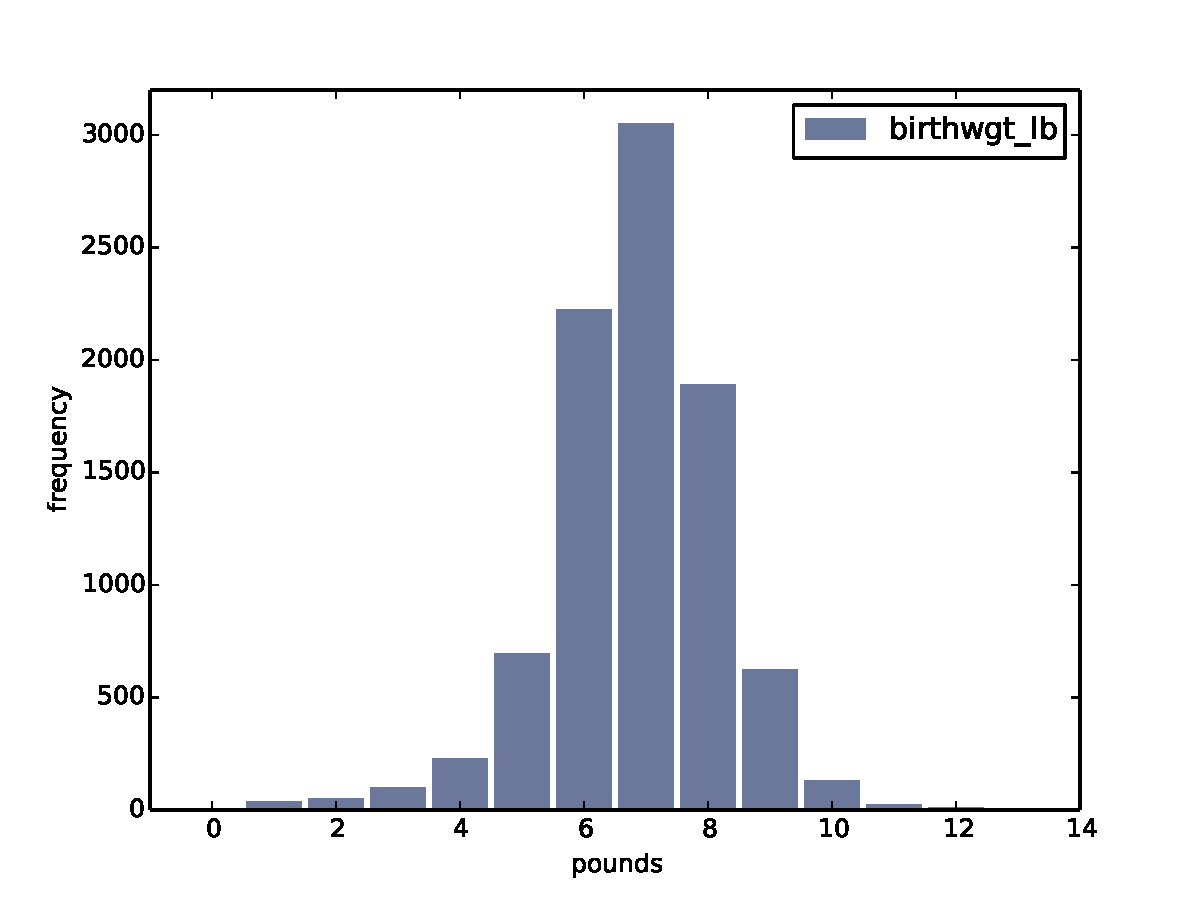
\includegraphics[height=2.5in]{figs/first_wgt_lb_hist.pdf}}
\caption{Histogram of the pound part of birth weight.}
\label{first_wgt_lb_hist}
\end{figure}

For this book I wrote a module called {\tt thinkplot.py} that provides
functions for plotting Hists and other objects defined in {\tt
  thinkstats2.py}.  It is based on {\tt pyplot}, which is part of the
{\tt matplotlib} package.  See Section~\ref{code} for information
about installing {\tt matplotlib}.  \index{thinkplot}
\index{matplotlib}

To plot {\tt hist} with {\tt thinkplot}, try this:
\index{Hist}

\begin{verbatim}
>>> import thinkplot
>>> thinkplot.Hist(hist)
>>> thinkplot.Show(xlabel='value', ylabel='frequency')
\end{verbatim}

You can read the documentation for {\tt thinkplot} at
\url{http://greenteapress.com/thinkstats2/thinkplot.html}.


\begin{figure}
% first.py
\centerline{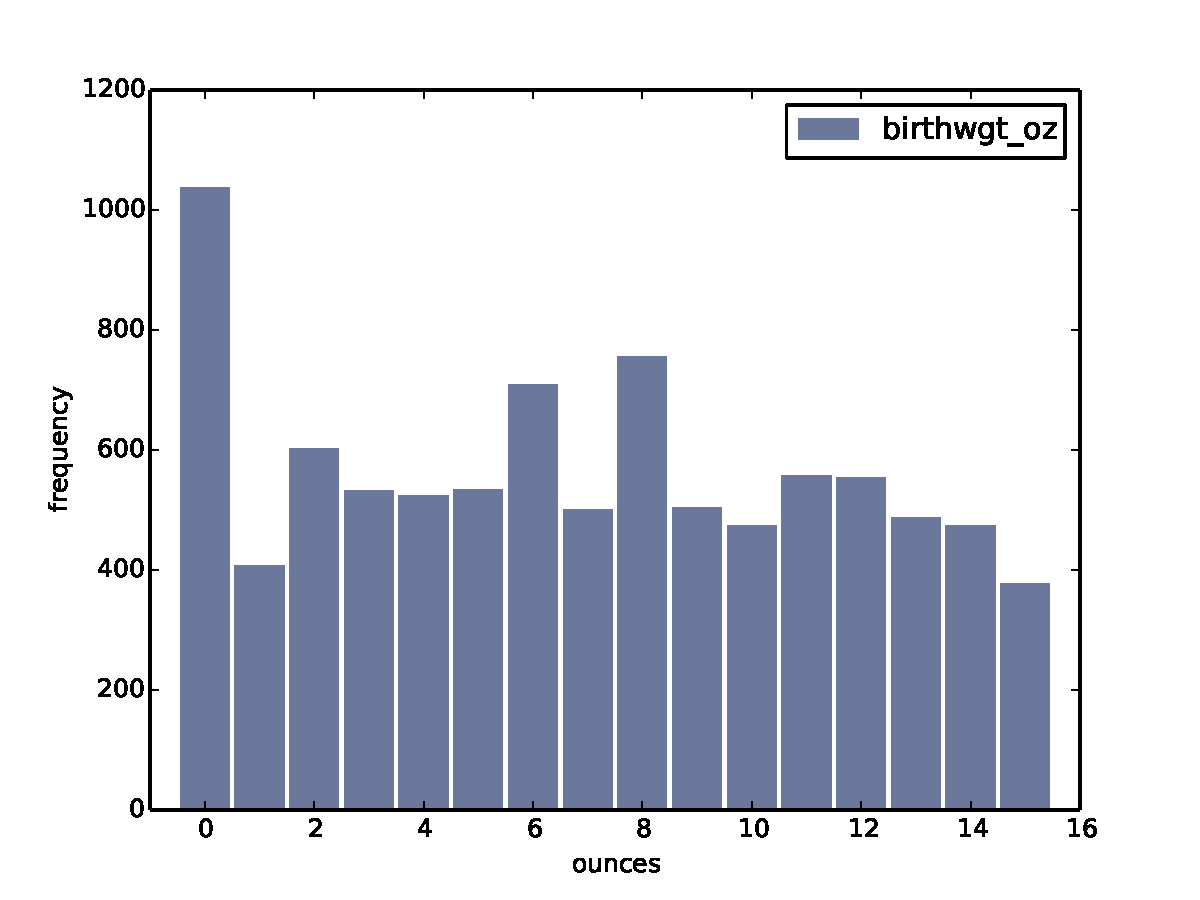
\includegraphics[height=2.5in]{figs/first_wgt_oz_hist.pdf}}
\caption{Histogram of the ounce part of birth weight.}
\label{first_wgt_oz_hist}
\end{figure}


\section{NSFG variables}

Now let's get back to the data from the NSFG.  The code in this
chapter is in {\tt first.py}.  
For information about downloading and
working with this code, see Section~\ref{code}.

When you start working with a new dataset, I suggest you explore
the variables you are planning to use one at a time, and a good
way to start is by looking at histograms.
\index{histogram}

In Section~\ref{cleaning} we transformed {\tt agepreg}
from centiyears to years, and combined \verb"birthwgt_lb" and
\verb"birthwgt_oz" into a single quantity, \verb"totalwgt_lb".
In this section I use these variables to demonstrate some
features of histograms.

\begin{figure}
% first.py
\centerline{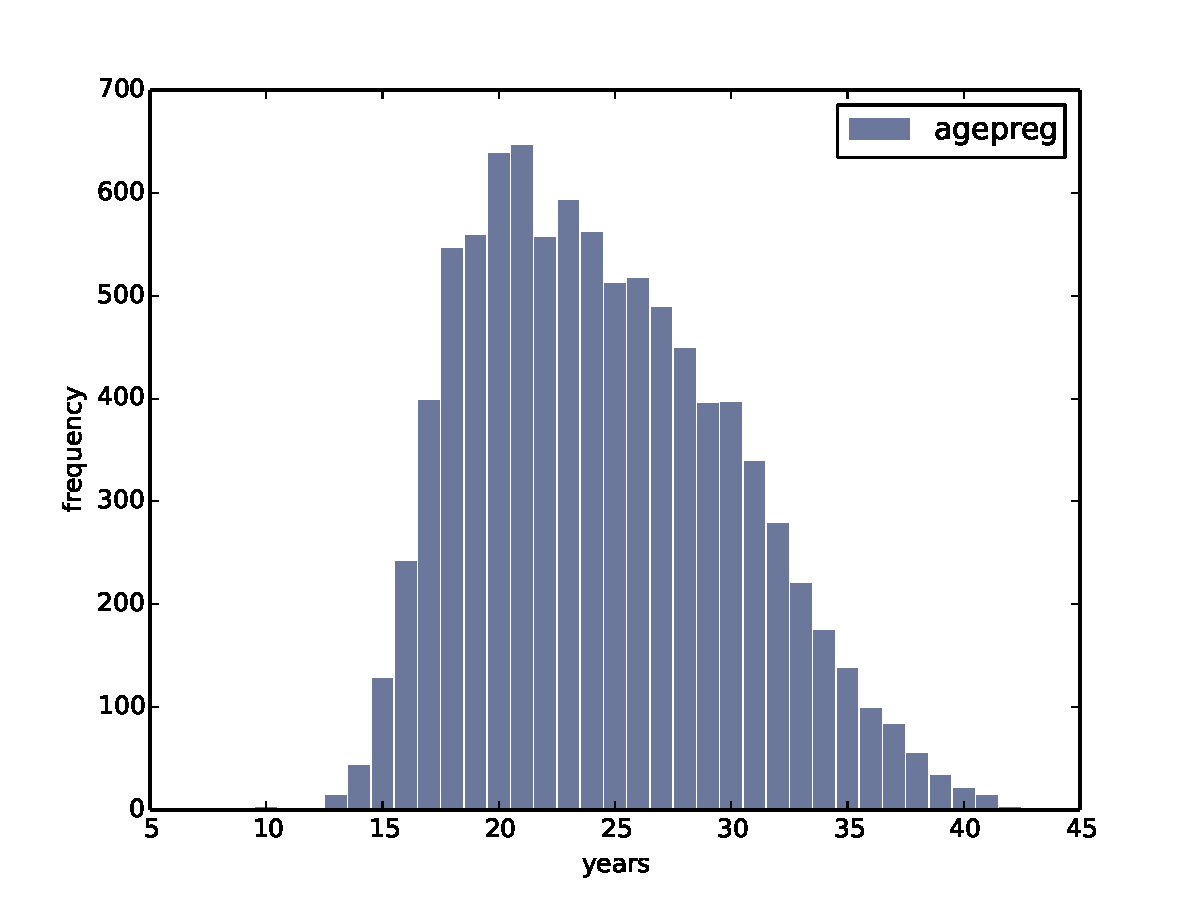
\includegraphics[height=2.5in]{figs/first_agepreg_hist.pdf}}
\caption{Histogram of mother's age at end of pregnancy.}
\label{first_agepreg_hist}
\end{figure}

I'll start by reading the data and selecting records for live
births:

\begin{verbatim}
    preg = nsfg.ReadFemPreg()
    live = preg[preg.outcome == 1]
\end{verbatim}

The expression in brackets is a boolean Series that
selects rows from the DataFrame and returns a new DataFrame.
Next I generate and plot the histogram of
\verb"birthwgt_lb" for live births.
\index{DataFrame}
\index{Series}
\index{Hist}
\index{bracket operator}
\index{boolean}

\begin{verbatim}
    hist = thinkstats2.Hist(live.birthwgt_lb, label='birthwgt_lb')
    thinkplot.Hist(hist)
    thinkplot.Show(xlabel='pounds', ylabel='frequency')
\end{verbatim}

When the argument passed to Hist is a pandas Series, any
{\tt nan} values are dropped.  {\tt label} is a string that appears
in the legend when the Hist is plotted.
\index{pandas}
\index{Series}
\index{thinkplot}
\index{NaN}

\begin{figure}
% first.py
\centerline{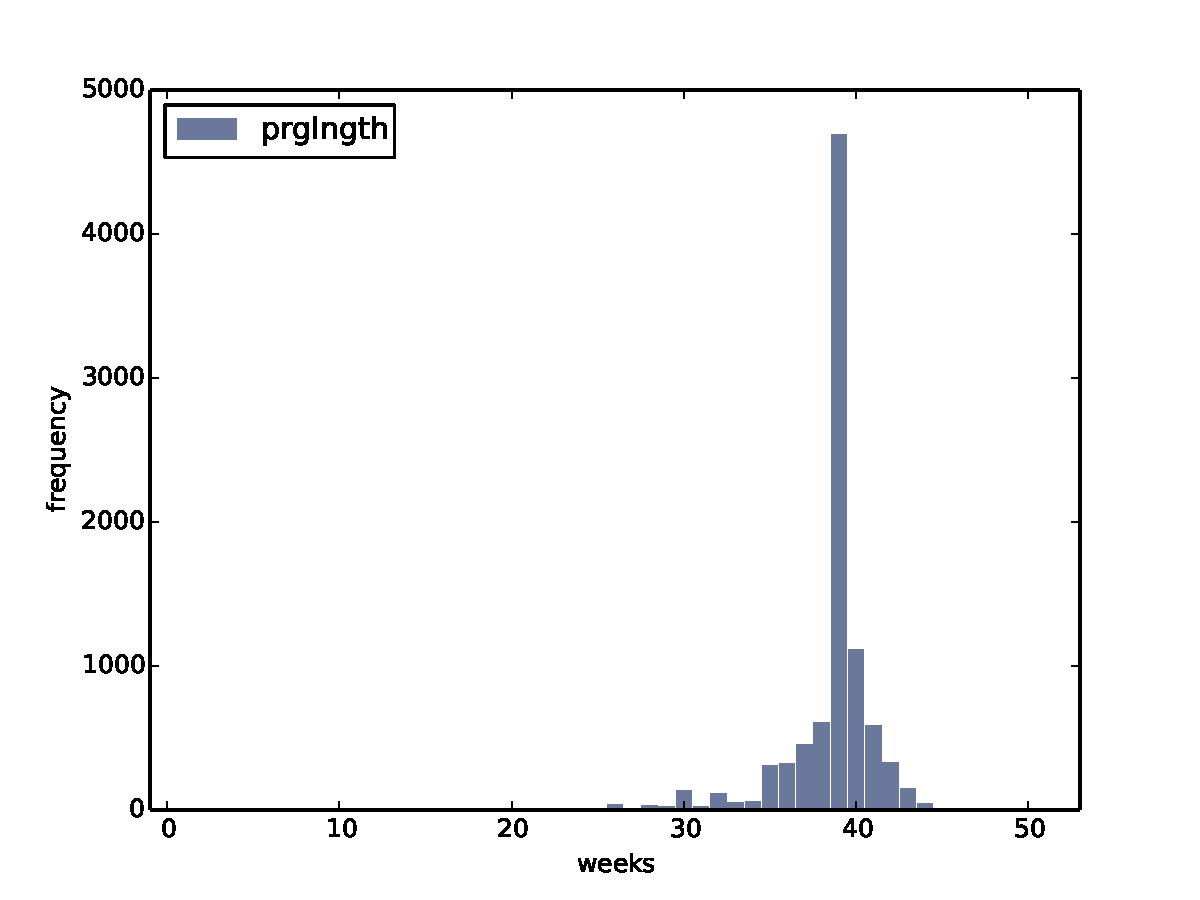
\includegraphics[height=2.5in]{figs/first_prglngth_hist.pdf}}
\caption{Histogram of pregnancy length in weeks.}
\label{first_prglngth_hist}
\end{figure}

Figure~\ref{first_wgt_lb_hist} shows the result.  The most common
value, called the {\bf mode}, is 7 pounds.  The distribution is
approximately bell-shaped, which is the shape of the {\bf normal}
distribution, also called a {\bf Gaussian} distribution.  But unlike a
true normal distribution, this distribution is asymmetric; it has
a {\bf tail} that extends farther to the left than to the right.

Figure~\ref{first_wgt_oz_hist} shows the histogram of
\verb"birthwgt_oz", which is the ounces part of birth weight.  In
theory we expect this distribution to be {\bf uniform}; that is, all
values should have the same frequency.  In fact, 0 is more common than
the other values, and 1 and 15 are less common, probably because
respondents round off birth weights that are close to an integer
value.
\index{birth weight}
\index{weight!birth}

Figure~\ref{first_agepreg_hist} shows the histogram of \verb"agepreg",
the mother's age at the end of pregnancy.  The mode is 21 years.  The
distribution is very roughly bell-shaped, but in this case the tail
extends farther to the right than left; most mothers are in
their 20s, fewer in their 30s.

Figure~\ref{first_prglngth_hist} shows the histogram of
\verb"prglngth", the length of the pregnancy in weeks.  By far the
most common value is 39 weeks.  The left tail is longer than the
right; early babies are common, but pregnancies seldom go past 43
weeks, and doctors often intervene if they do.
\index{pregnancy length}


\section{Outliers}

Looking at histograms, it is easy to identify the most common
values and the shape of the distribution, but rare values are
not always visible.
\index{histogram}

Before going on, it is a good idea to check for {\bf
  outliers}, which are extreme values that might be errors in
measurement and recording, or might be accurate reports of rare
events.
\index{outlier}

Hist provides methods {\tt Largest} and {\tt Smallest}, which take
an integer {\tt n} and return the {\tt n} largest or smallest
values from the histogram:
\index{Hist}

\begin{verbatim}
    for weeks, freq in hist.Smallest(10):
        print(weeks, freq)
\end{verbatim}

In the list of pregnancy lengths for live births, the 10 lowest values
are {\tt [0, 4, 9, 13, 17, 18, 19, 20, 21, 22]}.  Values below 10 weeks
are certainly errors; the most likely explanation is that the outcome
was not coded correctly.  Values higher than 30 weeks are probably
legitimate.  Between 10 and 30 weeks, it is hard to be sure; some
values are probably errors, but some represent premature babies.
\index{pregnancy length}

On the other end of the range, the highest values are:
%
\begin{verbatim}
weeks  count
43     148
44     46
45     10
46     1
47     1
48     7
50     2
\end{verbatim}

Most doctors recommend induced labor if a pregnancy exceeds 42 weeks,
so some of the longer values are surprising.  In particular, 50 weeks
seems medically unlikely.

The best way to handle outliers depends on ``domain knowledge'';
that is, information about where the data come from and what they
mean.  And it depends on what analysis you are planning to perform.
\index{outlier}

In this example, the motivating question is whether first babies
tend to be early (or late).  When people ask this question, they are
usually interested in full-term pregnancies, so for this analysis
I will focus on pregnancies longer than 27 weeks.


\section{First babies}

Now we can compare the distribution of pregnancy lengths for first
babies and others.  I divided the DataFrame of live births using
{\tt birthord}, and computed their histograms:
\index{DataFrame}
\index{Hist}
\index{pregnancy length}

\begin{verbatim}
    firsts = live[live.birthord == 1]
    others = live[live.birthord != 1]

    first_hist = thinkstats2.Hist(firsts.prglngth)
    other_hist = thinkstats2.Hist(others.prglngth)
\end{verbatim}

Then I plotted their histograms on the same axis:

\begin{verbatim}
    width = 0.45
    thinkplot.PrePlot(2)
    thinkplot.Hist(first_hist, align='right', width=width)
    thinkplot.Hist(other_hist, align='left', width=width)
    thinkplot.Show(xlabel='weeks', ylabel='frequency')
\end{verbatim}

{\tt thinkplot.PrePlot} takes the number of histograms
we are planning to plot; it uses this information to choose
an appropriate collection of colors.
\index{thinkplot}

\begin{figure}
% first.py
\centerline{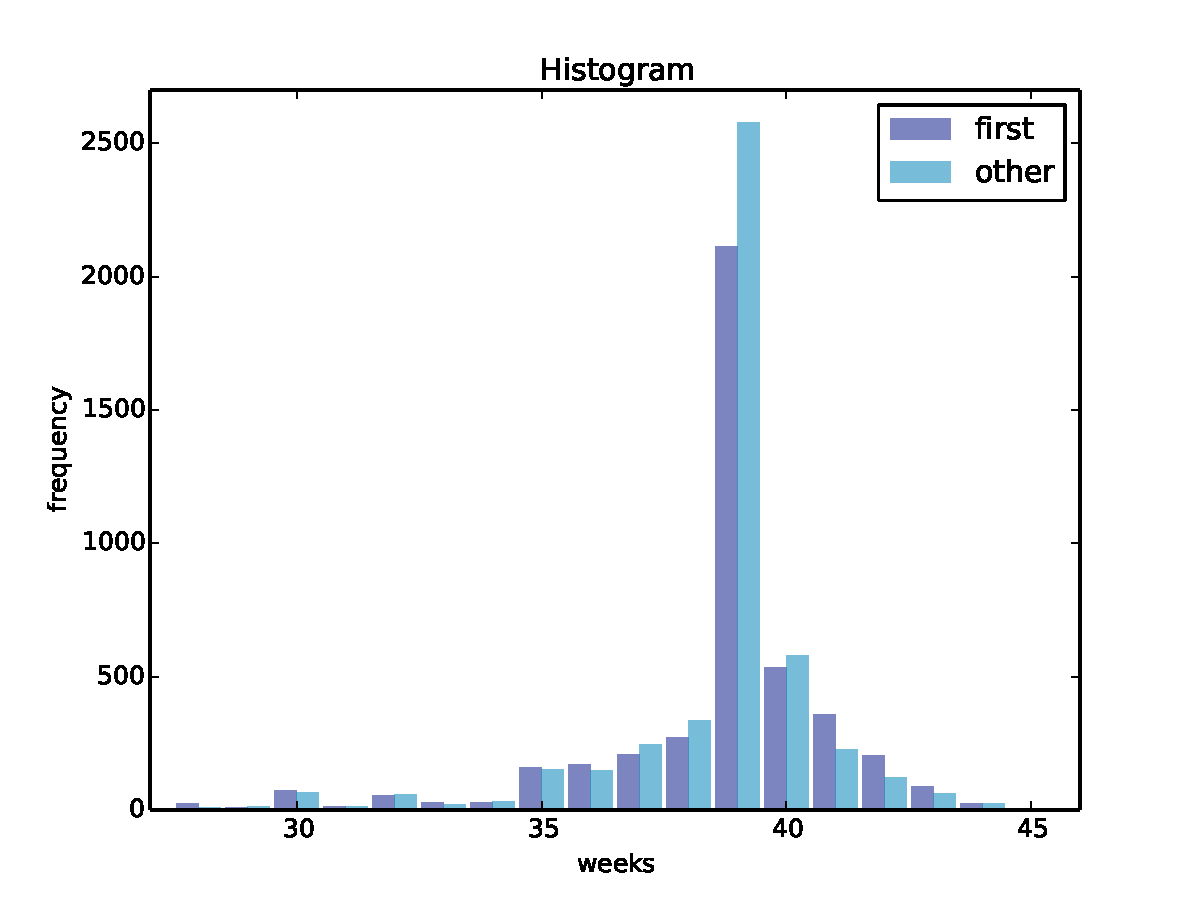
\includegraphics[height=2.5in]{figs/first_nsfg_hist.pdf}}
\caption{Histogram of pregnancy lengths.}
\label{first_nsfg_hist}
\end{figure}

{\tt thinkplot.Hist} normally uses {\tt align='center'} so that
each bar is centered over its value.  For this figure, I use
{\tt align='right'} and {\tt align='left'} to place
corresponding bars on either side of the value.
\index{Hist}

With {\tt width=0.45}, the total width of the two bars is 0.9,
leaving some space between each pair.

Finally, I adjust the axis to show only data between 27 and 46 weeks.
Figure~\ref{first_nsfg_hist} shows the result.
\index{pregnancy length}
\index{length!pregnancy}

Histograms are useful because they make the most frequent values
immediately apparent.  But they are not the best choice for comparing
two distributions.  In this example, there are fewer ``first babies''
than ``others,'' so some of the apparent differences in the histograms
are due to sample sizes.  In the next chapter we address this problem
using probability mass functions.


\section{Summarizing distributions}
\label{mean}

A histogram is a complete description of the distribution of a sample;
that is, given a histogram, we could reconstruct the values in the
sample (although not their order).

If the details of the distribution are important, it might be
necessary to present a histogram.  But often we want to
summarize the distribution with a few descriptive statistics.

Some of the characteristics we might want to report are:

\begin{itemize}

\item central tendency: Do the values tend to cluster around
a particular point?
\index{central tendency}

\item modes: Is there more than one cluster?
\index{mode}

\item spread: How much variability is there in the values?
\index{spread}

\item tails: How quickly do the probabilities drop off as we
move away from the modes?
\index{tail}

\item outliers: Are there extreme values far from the modes?
\index{outlier}

\end{itemize}

Statistics designed to answer these questions are called {\bf summary
  statistics}.  By far the most common summary statistic is the {\bf
  mean}, which is meant to describe the central tendency of the
distribution.  \index{mean} \index{average} \index{summary statistic}

If you have a sample of {\tt n} values, $x_i$, the mean, $\xbar$, is
the sum of the values divided by the number of values; in other words
%
\[ \xbar = \frac{1}{n} \sum_i x_i \]
%
The words ``mean'' and ``average'' are sometimes used interchangeably,
but I make this distinction:

\begin{itemize}

\item The ``mean'' of a sample is the summary statistic computed with
  the previous formula.

\item An ``average'' is one of several summary statistics you might
  choose to describe a central tendency.
\index{central tendency}

\end{itemize}

Sometimes the mean is a good description of a set of values.  For
example, apples are all pretty much the same size (at least the ones
sold in supermarkets).  So if I buy 6 apples and the total weight is 3
pounds, it would be a reasonable summary to say they are about a half
pound each.
\index{weight!pumpkin}

But pumpkins are more diverse.  Suppose I grow several varieties in my
garden, and one day I harvest three decorative pumpkins that are 1
pound each, two pie pumpkins that are 3 pounds each, and one Atlantic
Giant\textregistered~pumpkin that weighs 591 pounds.  The mean of this
sample is 100 pounds, but if I told you ``The average pumpkin in my
garden is 100 pounds,'' that would be misleading.  In this example,
there is no meaningful average because there is no typical pumpkin.
\index{pumpkin}



\section{Variance}
\index{variance}

If there is no single number that summarizes pumpkin weights,
we can do a little better with two numbers: mean and {\bf variance}.

Variance is a summary statistic intended to describe the variability
or spread of a distribution.  The variance of a set of values is
%
\[ S^2 = \frac{1}{n} \sum_i (x_i - \xbar)^2 \]
%
The term $x_i - \xbar$ is called the ``deviation from the mean,'' so
variance is the mean squared deviation.  The square root of variance,
$S$, is the {\bf standard deviation}.  \index{deviation}
\index{standard deviation}
\index{deviation}

If you have prior experience, you might have seen a formula for
variance with $n-1$ in the denominator, rather than {\tt n}.  This
statistic is used to estimate the variance in a population using a
sample.  We will come back to this in Chapter~\ref{estimation}.
\index{sample variance}

Pandas data structures provides methods to compute mean, variance and
standard deviation:
\index{pandas}

\begin{verbatim}
    mean = live.prglngth.mean()
    var = live.prglngth.var()
    std = live.prglngth.std()
\end{verbatim}

For all live births, the mean pregnancy length is 38.6 weeks, the
standard deviation is 2.7 weeks, which means we should expect
deviations of 2-3 weeks to be common.
\index{pregnancy length}

Variance of pregnancy length is 7.3, which is hard to interpret,
especially since the units are weeks$^2$, or ``square weeks.''
Variance is useful in some calculations, but it is not
a good summary statistic.


\section{Effect size}
\index{effect size}

An {\bf effect size} is a summary statistic intended to describe (wait
for it) the size of an effect.  For example, to describe the
difference between two groups, one obvious choice is the difference in
the means.  \index{effect size}

Mean pregnancy length for first babies is 38.601; for
other babies it is 38.523.  The difference is 0.078 weeks, which works
out to 13 hours.  As a fraction of the typical pregnancy length, this
difference is about 0.2\%.
\index{pregnancy length}

If we assume this estimate is accurate, such a difference
would have no practical consequences.  In fact, without
observing a large number of pregnancies, it is unlikely that anyone
would notice this difference at all.
\index{effect size}

Another way to convey the size of the effect is to compare the
difference between groups to the variability within groups.
Cohen's $d$ is a statistic intended to do that; it is defined
%
\[ d = \frac{\bar{x_1} - \bar{x_2}}{s}  \]
%
where $\bar{x_1}$ and $\bar{x_2}$ are the means of the groups and
$s$ is the ``pooled standard deviation''.  Here's the Python
code that computes Cohen's $d$:
\index{standard deviation!pooled}

\begin{verbatim}
def CohenEffectSize(group1, group2):
    diff = group1.mean() - group2.mean()

    var1 = group1.var()
    var2 = group2.var()
    n1, n2 = len(group1), len(group2)

    pooled_var = (n1 * var1 + n2 * var2) / (n1 + n2)
    d = diff / math.sqrt(pooled_var)
    return d
\end{verbatim}

In this example, the difference in means is 0.029 standard deviations,
which is small.  To put that in perspective, the difference in
height between men and women is about 1.7 standard deviations (see
\url{https://en.wikipedia.org/wiki/Effect_size}).


\section{Reporting results}

We have seen several ways to describe the difference in pregnancy
length (if there is one) between first babies and others.  How should
we report these results?
\index{pregnancy length}

The answer depends on who is asking the question.  A scientist might
be interested in any (real) effect, no matter how small.  A doctor
might only care about effects that are {\bf clinically significant};
that is, differences that affect treatment decisions.  A pregnant
woman might be interested in results that are relevant to her, like
the probability of delivering early or late.
\index{clinically significant} \index{significant}

How you report results also depends on your goals.  If you are trying
to demonstrate the importance of an effect, you might choose summary
statistics that emphasize differences.  If you are trying to reassure
a patient, you might choose statistics that put the differences in
context.

Of course your decisions should also be guided by professional ethics.
It's ok to be persuasive; you {\em should} design statistical reports
and visualizations that tell a story clearly.  But you should also do
your best to make your reports honest, and to acknowledge uncertainty
and limitations.
\index{ethics}


\section{Exercises}

\begin{exercise}
Based on the results in this chapter, suppose you were asked to
summarize what you learned about whether first babies arrive late.

Which summary statistics would you use if you wanted to get a story
on the evening news?  Which ones would you use if you wanted to
reassure an anxious patient?
\index{Adams, Cecil}
\index{Straight Dope, The}

Finally, imagine that you are Cecil Adams, author of {\it The Straight
  Dope} (\url{http://straightdope.com}), and your job is to answer the
question, ``Do first babies arrive late?''  Write a paragraph that
uses the results in this chapter to answer the question clearly,
precisely, and honestly.
\index{ethics}

\end{exercise}

\begin{exercise}
In the repository you downloaded, you should find a file named
\verb"chap02ex.ipynb"; open it.  Some cells are already filled in, and
you should execute them.  Other cells give you instructions for
exercises.  Follow the instructions and fill in the answers.

A solution to this exercise is in \verb"chap02soln.ipynb"
\end{exercise}

In the repository you downloaded, you should find a file named
\verb"chap02ex.py"; you can use this file as a starting place
for the following exercises.
My solution is in \verb"chap02soln.py".

\begin{exercise}
The mode of a distribution is the most frequent value; see
\url{http://wikipedia.org/wiki/Mode_(statistics)}.  Write a function
called {\tt Mode} that takes a Hist and returns the most
frequent value.\index{mode}
\index{Hist}

As a more challenging exercise, write a function called {\tt AllModes}
that returns a list of value-frequency pairs in descending order of
frequency.
\index{frequency}
\end{exercise}

\begin{exercise}
Using the variable \verb"totalwgt_lb", investigate whether first
babies are lighter or heavier than others.  Compute Cohen's $d$
to quantify the difference between the groups.  How does it
compare to the difference in pregnancy length?
\index{pregnancy length}
\end{exercise}


\section{Glossary}

\begin{itemize}

\item distribution: The values that appear in a sample
and the frequency of each.
\index{distribution}

\item histogram: A mapping from values to frequencies, or a graph
that shows this mapping.
\index{histogram}

\item frequency: The number of times a value appears in a sample.
\index{frequency}

\item mode: The most frequent value in a sample, or one of the
most frequent values.
\index{mode}

\item normal distribution: An idealization of a bell-shaped distribution;
also known as a Gaussian distribution. 
\index{Gaussian distribution}
\index{normal distribution}

\item uniform distribution: A distribution in which all values have
the same frequency.
\index{uniform distribution}

\item tail: The part of a distribution at the high and low extremes.
\index{tail}

\item central tendency: A characteristic of a sample or population;
intuitively, it is an average or typical value. 
\index{central tendency}

\item outlier: A value far from the central tendency.
\index{outlier}

\item spread: A measure of how spread out the values in a distribution
are.
\index{spread}

\item summary statistic: A statistic that quantifies some aspect
of a distribution, like central tendency or spread.
\index{summary statistic}

\item variance: A summary statistic often used to quantify spread.
\index{variance}

\item standard deviation: The square root of variance, also used
as a measure of spread.
\index{standard deviation}

\item effect size: A summary statistic intended to quantify the size
of an effect like a difference between groups.
\index{effect size}

\item clinically significant: A result, like a difference between groups,
that is relevant in practice.
\index{clinically significant}

\end{itemize}




\chapter{Probability mass functions}
\index{probability mass function}

The code for this chapter is in {\tt probability.py}.
For information about downloading and
working with this code, see Section~\ref{code}.


\section{Pmfs}
\index{Pmf}

Another way to represent a distribution is a {\bf probability mass
  function} (PMF), which maps from each value to its probability.  A
{\bf probability} is a frequency expressed as a fraction of the sample
size, {\tt n}.  To get from frequencies to probabilities, we divide
through by {\tt n}, which is called {\bf normalization}.
\index{frequency}
\index{probability}
\index{normalization}
\index{PMF}
\index{probability mass function}

Given a Hist, we can make a dictionary that maps from each
value to its probability: \index{Hist}
%
\begin{verbatim}
n = hist.Total()
d = {}
for x, freq in hist.Items():
    d[x] = freq / n
\end{verbatim}
%
Or we can use the Pmf class provided by {\tt thinkstats2}.
Like Hist, the Pmf constructor can take a list, pandas
Series, dictionary, Hist, or another Pmf object.  Here's an example
with a simple list:
%
\begin{verbatim}
>>> import thinkstats2
>>> pmf = thinkstats2.Pmf([1, 2, 2, 3, 5])
>>> pmf
Pmf({1: 0.2, 2: 0.4, 3: 0.2, 5: 0.2})
\end{verbatim}

The Pmf is normalized so total probability is 1.

Pmf and Hist objects are similar in many ways; in fact, they inherit
many of their methods from a common parent class.  For example, the
methods {\tt Values} and {\tt Items} work the same way for both.  The
biggest difference is that a Hist maps from values to integer
counters; a Pmf maps from values to floating-point probabilities.
\index{Hist}

To look up the probability associated with a value, use {\tt Prob}:
%
\begin{verbatim}
>>> pmf.Prob(2)
0.4
\end{verbatim}

The bracket operator is equivalent:
\index{bracket operator}

\begin{verbatim}
>>> pmf[2]
0.4
\end{verbatim}

You can modify an existing Pmf by incrementing the probability
associated with a value:
%
\begin{verbatim}
>>> pmf.Incr(2, 0.2)
>>> pmf.Prob(2)
0.6
\end{verbatim}

Or you can multiply a probability by a factor:
%
\begin{verbatim}
>>> pmf.Mult(2, 0.5)
>>> pmf.Prob(2)
0.3
\end{verbatim}

If you modify a Pmf, the result may not be normalized; that is, the
probabilities may no longer add up to 1.  To check, you can call {\tt
  Total}, which returns the sum of the probabilities:
%
\begin{verbatim}
>>> pmf.Total()
0.9
\end{verbatim}

To renormalize, call {\tt Normalize}:
%
\begin{verbatim}
>>> pmf.Normalize()
>>> pmf.Total()
1.0
\end{verbatim}

Pmf objects provide a {\tt Copy} method so you can make
and modify a copy without affecting the original.
\index{Pmf}

My notation in this section might seem inconsistent, but there is a
system: I use Pmf for the name of the class, {\tt pmf} for an instance
of the class, and PMF for the mathematical concept of a
probability mass function.


\section{Plotting PMFs}
\index{PMF}

{\tt thinkplot} provides two ways to plot Pmfs:
\index{thinkplot}

\begin{itemize}

\item To plot a Pmf as a bar graph, you can use 
{\tt thinkplot.Hist}.  Bar graphs are most useful if the number
of values in the Pmf is small.
\index{bar plot}
\index{plot!bar}

\item To plot a Pmf as a step function, you can use
{\tt thinkplot.Pmf}.  This option is most useful if there are
a large number of values and the Pmf is smooth.  This function
also works with Hist objects.
\index{line plot}
\index{plot!line}
\index{Hist}
\index{Pmf}

\end{itemize}

In addition, {\tt pyplot} provides a function called {\tt hist} that
takes a sequence of values, computes a histogram, and plots it.
Since I use Hist objects, I usually don't use {\tt pyplot.hist}.
\index{pyplot}

\begin{figure}
% probability.py
\centerline{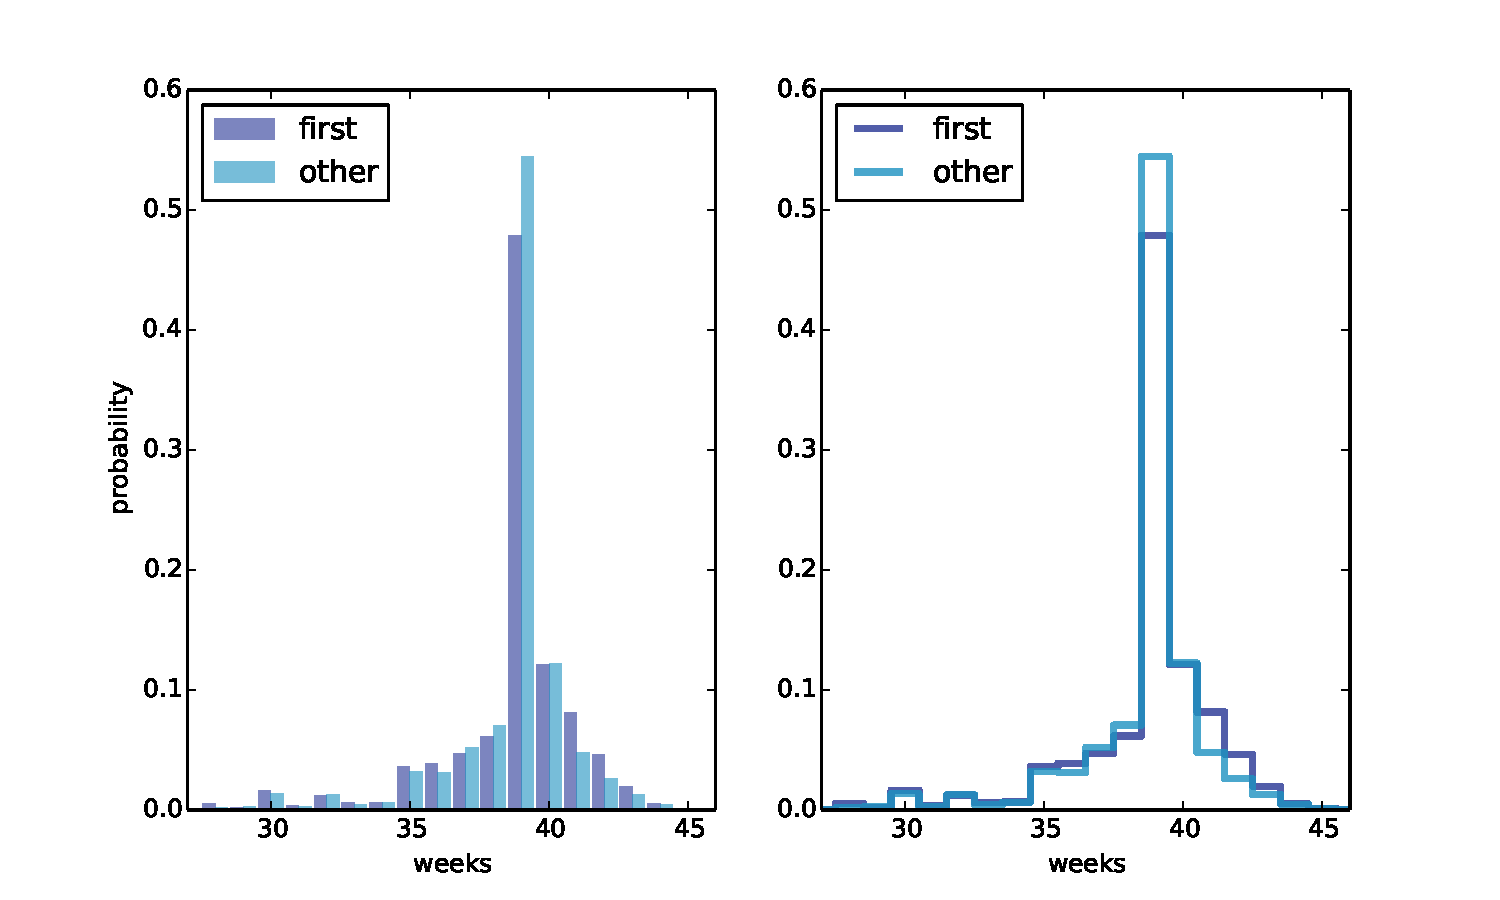
\includegraphics[height=3.0in]{figs/probability_nsfg_pmf.pdf}}
\caption{PMF of pregnancy lengths for first babies and others, using
  bar graphs and step functions.}
\label{probability_nsfg_pmf}
\end{figure}
\index{pregnancy length}
\index{length!pregnancy}

Figure~\ref{probability_nsfg_pmf} shows PMFs of pregnancy length for
first babies and others using bar graphs (left) and step functions
(right).
\index{pregnancy length}

By plotting the PMF instead of the histogram, we can compare the two
distributions without being mislead by the difference in sample
size.  Based on this figure, first babies seem to be less likely than
others to arrive on time (week 39) and more likely to be a late (weeks
41 and 42).

Here's the code that generates Figure~\ref{probability_nsfg_pmf}:

\begin{verbatim}
    thinkplot.PrePlot(2, cols=2)
    thinkplot.Hist(first_pmf, align='right', width=width)
    thinkplot.Hist(other_pmf, align='left', width=width)
    thinkplot.Config(xlabel='weeks',
                     ylabel='probability',
                     axis=[27, 46, 0, 0.6])

    thinkplot.PrePlot(2)
    thinkplot.SubPlot(2)
    thinkplot.Pmfs([first_pmf, other_pmf])
    thinkplot.Show(xlabel='weeks',
                   axis=[27, 46, 0, 0.6])
\end{verbatim}

{\tt PrePlot} takes optional parameters {\tt rows} and {\tt cols}
to make a grid of figures, in this case one row of two figures.
The first figure (on the left) displays the Pmfs using {\tt thinkplot.Hist},
as we have seen before.
\index{thinkplot}
\index{Hist}

The second call to {\tt PrePlot} resets the color generator.  Then
{\tt SubPlot} switches to the second figure (on the right) and
displays the Pmfs using {\tt thinkplot.Pmfs}.  I used the {\tt axis} option
to ensure that the two figures are on the same axes, which is
generally a good idea if you intend to compare two figures.


\section{Other visualizations}
\label{visualization}

Histograms and PMFs are useful while you are exploring data and
trying to identify patterns and relationships.
Once you have an idea what is going on, a good next step is to
design a visualization that makes the patterns you have identified
as clear as possible.
\index{exploratory data analysis}
\index{visualization}

In the NSFG data, the biggest differences in the distributions are
near the mode.  So it makes sense to zoom in on that part of the
graph, and to transform the data to emphasize differences:
\index{National Survey of Family Growth}
\index{NSFG}

\begin{verbatim}
    weeks = range(35, 46)
    diffs = []
    for week in weeks:
        p1 = first_pmf.Prob(week)
        p2 = other_pmf.Prob(week)
        diff = 100 * (p1 - p2)
        diffs.append(diff)

    thinkplot.Bar(weeks, diffs)
\end{verbatim}

In this code, {\tt weeks} is the range of weeks; {\tt diffs} is the
difference between the two PMFs in percentage points.
Figure~\ref{probability_nsfg_diffs} shows the result as a bar chart.
This figure makes the pattern clearer: first babies are less likely to
be born in week 39, and somewhat more likely to be born in weeks 41
and 42.
\index{thinkplot}

\begin{figure}
% probability.py
\centerline{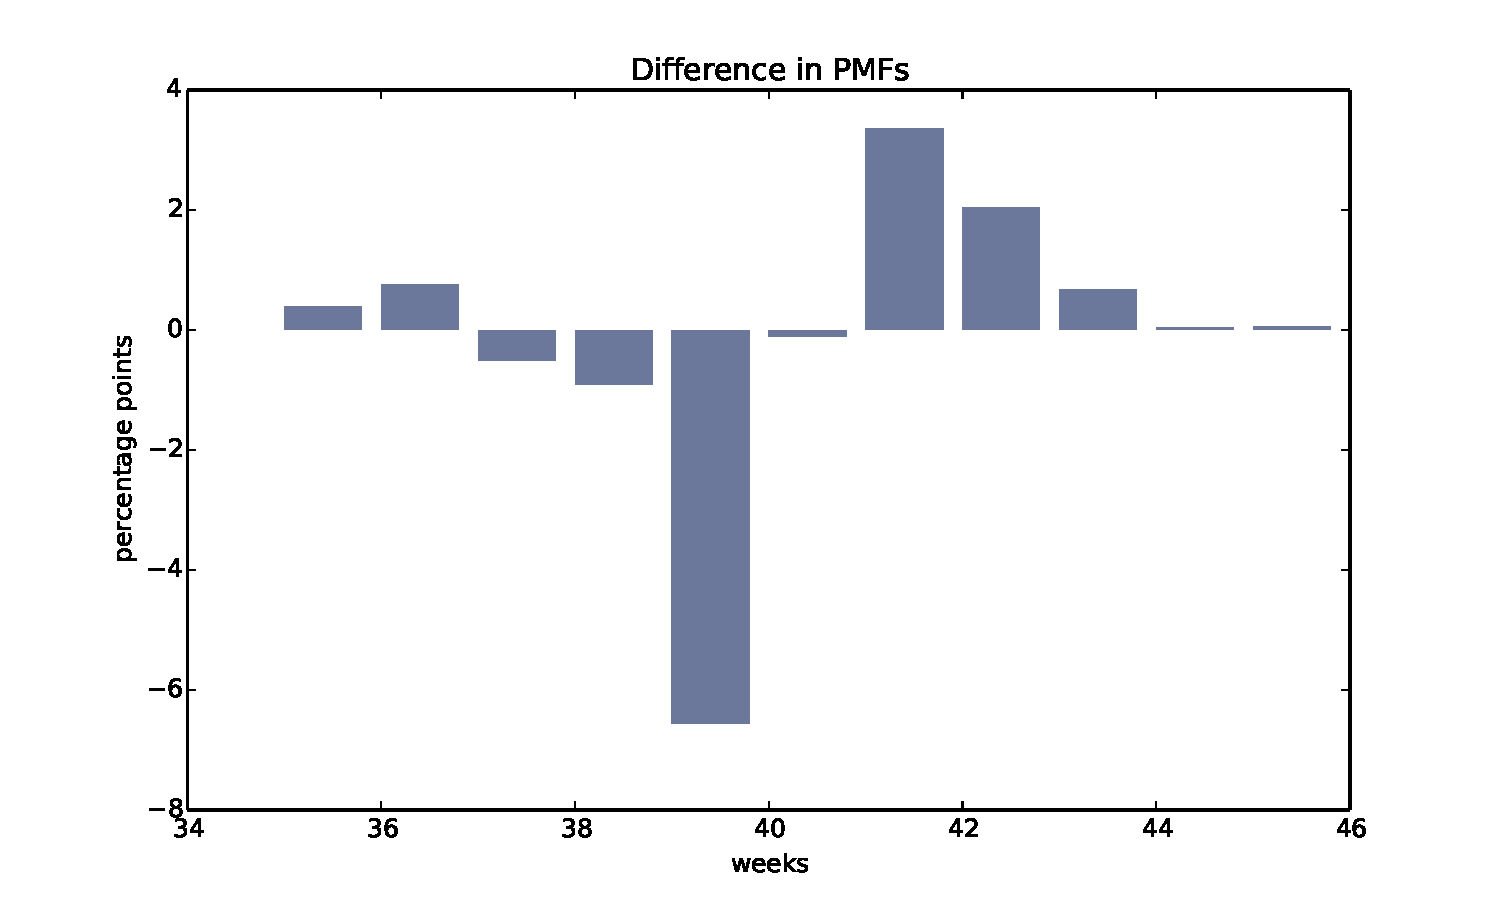
\includegraphics[height=2.5in]{figs/probability_nsfg_diffs.pdf}}
\caption{Difference, in percentage points, by week.}
\label{probability_nsfg_diffs}
\end{figure}

For now we should hold this conclusion only tentatively.
We used the same dataset to identify an
apparent difference and then chose a visualization that makes the
difference apparent.  We can't be sure this effect is real;
it might be due to random variation.  We'll address this concern
later.


\section{The class size paradox}
\index{class size}

Before we go on, I want to demonstrate
one kind of computation you can do with Pmf objects; I call
this example the ``class size paradox.''
\index{Pmf}

At many American colleges and universities, the student-to-faculty
ratio is about 10:1.  But students are often surprised to discover
that their average class size is bigger than 10.  There
are two reasons for the discrepancy:

\begin{itemize}

\item Students typically take 4--5 classes per semester, but
professors often teach 1 or 2.

\item The number of students who enjoy a small class is small,
but the number of students in a large class is (ahem!) large.

\end{itemize}

The first effect is obvious, at least once it is pointed out;
the second is more subtle.  Let's look at an example.  Suppose
that a college offers 65 classes in a given semester, with the
following distribution of sizes:
%
\begin{verbatim}
 size      count
 5- 9          8
10-14          8
15-19         14
20-24          4
25-29          6
30-34         12
35-39          8
40-44          3
45-49          2
\end{verbatim}

If you ask the Dean for the average class size, he would
construct a PMF, compute the mean, and report that the
average class size is 23.7.  Here's the code:

\begin{verbatim}
    d = { 7: 8, 12: 8, 17: 14, 22: 4, 
          27: 6, 32: 12, 37: 8, 42: 3, 47: 2 }

    pmf = thinkstats2.Pmf(d, label='actual')
    print('mean', pmf.Mean())
\end{verbatim}

But if you survey a group of students, ask them how many
students are in their classes, and compute the mean, you would
think the average class was bigger.  Let's see how
much bigger.

First, I compute the
distribution as observed by students, where the probability
associated with each class size is ``biased'' by the number
of students in the class.
\index{observer bias}
\index{bias!observer}

\begin{verbatim}
def BiasPmf(pmf, label):
    new_pmf = pmf.Copy(label=label)

    for x, p in pmf.Items():
        new_pmf.Mult(x, x)
        
    new_pmf.Normalize()
    return new_pmf
\end{verbatim}

For each class size, {\tt x}, we multiply the probability by
{\tt x}, the number of students who observe that class size.
The result is a new Pmf that represents the biased distribution.

Now we can plot the actual and observed distributions:
\index{thinkplot}

\begin{verbatim}
    biased_pmf = BiasPmf(pmf, label='observed')
    thinkplot.PrePlot(2)
    thinkplot.Pmfs([pmf, biased_pmf])
    thinkplot.Show(xlabel='class size', ylabel='PMF')
\end{verbatim}

\begin{figure}
% probability.py
\centerline{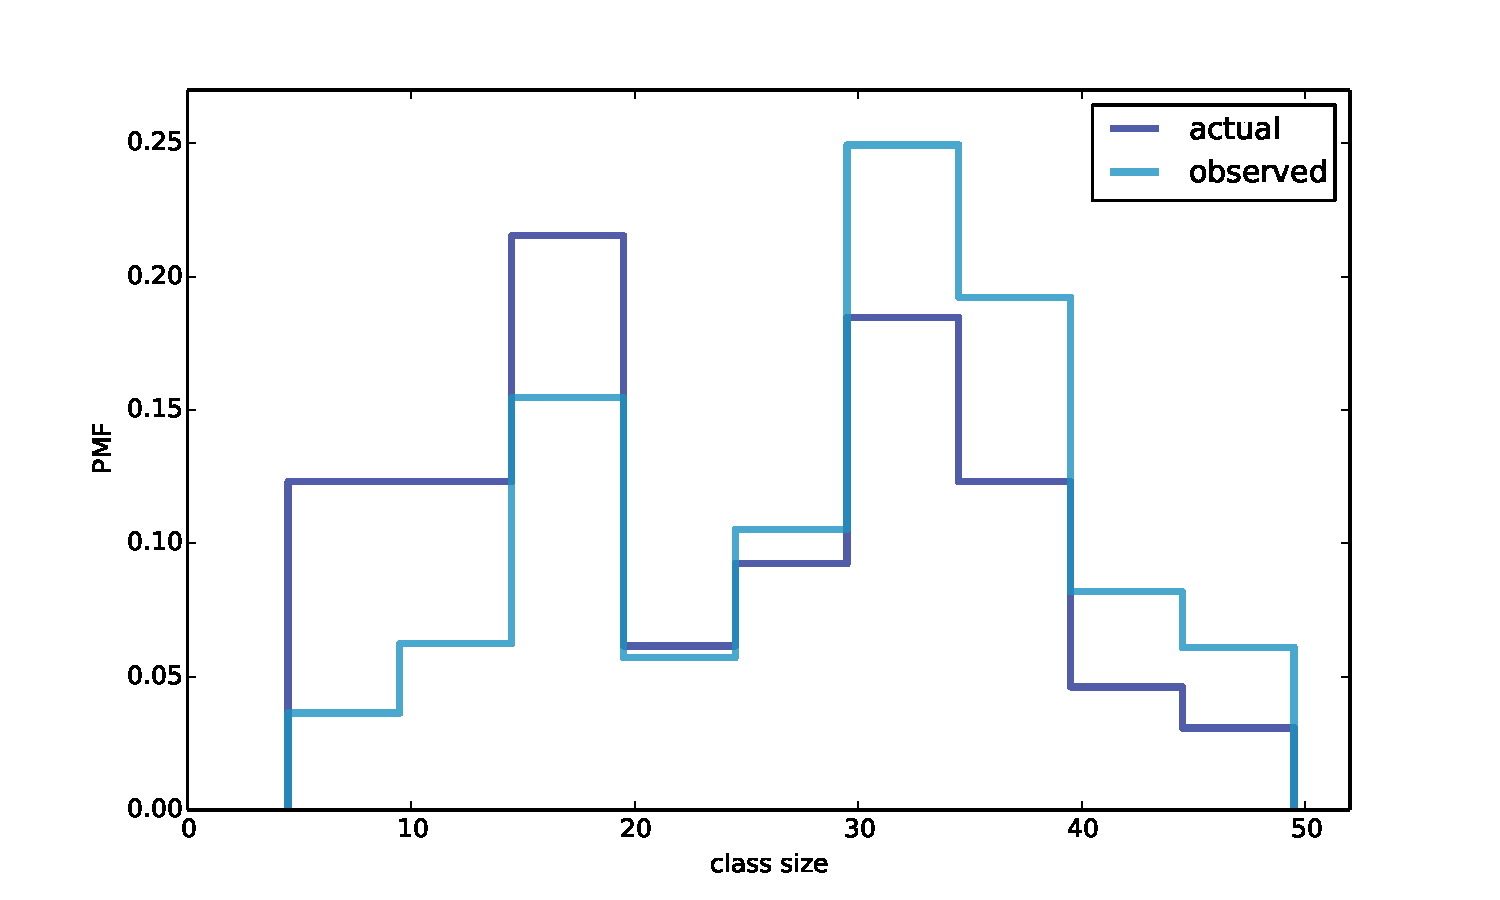
\includegraphics[height=3.0in]{figs/class_size1.pdf}}
\caption{Distribution of class sizes, actual and as observed by students.}
\label{class_size1}
\end{figure}

Figure~\ref{class_size1} shows the result.  In the biased distribution
there are fewer small classes and more large ones.
The mean of the biased distribution is 29.1, almost 25\% higher
than the actual mean.

It is also possible to invert this operation.  Suppose you want to
find the distribution of class sizes at a college, but you can't get
reliable data from the Dean.  An alternative is to choose a random
sample of students and ask how many students are in their
classes.  \index{bias!oversampling} \index{oversampling}

The result would be biased for the reasons we've just seen, but you
can use it to estimate the actual distribution.  Here's the function
that unbiases a Pmf:

\begin{verbatim}
def UnbiasPmf(pmf, label):
    new_pmf = pmf.Copy(label=label)

    for x, p in pmf.Items():
        new_pmf.Mult(x, 1.0/x)
        
    new_pmf.Normalize()
    return new_pmf
\end{verbatim}

It's similar to {\tt BiasPmf}; the only difference is that it
divides each probability by {\tt x} instead of multiplying.


\section{DataFrame indexing}

In Section~\ref{dataframe} we read a pandas DataFrame and used it to
select and modify data columns.  Now let's look at row selection.
To start, I create a NumPy array of random numbers and use it
to initialize a DataFrame:
\index{NumPy}
\index{pandas}
\index{DataFrame}

\begin{verbatim}
>>> import numpy as np
>>> import pandas
>>> array = np.random.randn(4, 2)
>>> df = pandas.DataFrame(array)
>>> df
          0         1
0 -0.143510  0.616050
1 -1.489647  0.300774
2 -0.074350  0.039621
3 -1.369968  0.545897
\end{verbatim}

By default, the rows and columns are numbered starting at zero, but
you can provide column names:

\begin{verbatim}
>>> columns = ['A', 'B']
>>> df = pandas.DataFrame(array, columns=columns)
>>> df
          A         B
0 -0.143510  0.616050
1 -1.489647  0.300774
2 -0.074350  0.039621
3 -1.369968  0.545897
\end{verbatim}

You can also provide row names.  The set of row names is called the
{\bf index}; the row names themselves are called {\bf labels}.

\begin{verbatim}
>>> index = ['a', 'b', 'c', 'd']
>>> df = pandas.DataFrame(array, columns=columns, index=index)
>>> df
          A         B
a -0.143510  0.616050
b -1.489647  0.300774
c -0.074350  0.039621
d -1.369968  0.545897
\end{verbatim}

As we saw in the previous chapter, simple indexing selects a
column, returning a Series:
\index{Series}

\begin{verbatim}
>>> df['A']
a   -0.143510
b   -1.489647
c   -0.074350
d   -1.369968
Name: A, dtype: float64
\end{verbatim}

To select a row by label, you can use the {\tt loc} attribute, which
returns a Series:

\begin{verbatim}
>>> df.loc['a']
A   -0.14351
B    0.61605
Name: a, dtype: float64
\end{verbatim}

If you know the integer position of a row, rather than its label, you
can use the {\tt iloc} attribute, which also returns a Series.

\begin{verbatim}
>>> df.iloc[0]
A   -0.14351
B    0.61605
Name: a, dtype: float64
\end{verbatim}

{\tt loc} can also take a list of labels; in that case,
the result is a DataFrame.

\begin{verbatim}
>>> indices = ['a', 'c']
>>> df.loc[indices]
         A         B
a -0.14351  0.616050
c -0.07435  0.039621
\end{verbatim}

Finally, you can use a slice to select a range of rows by label:

\begin{verbatim}
>>> df['a':'c']
          A         B
a -0.143510  0.616050
b -1.489647  0.300774
c -0.074350  0.039621
\end{verbatim}

Or by integer position:

\begin{verbatim}
>>> df[0:2]
          A         B
a -0.143510  0.616050
b -1.489647  0.300774
\end{verbatim}

The result in either case is a DataFrame, but notice that the first
result includes the end of the slice; the second doesn't.
\index{DataFrame}

My advice: if your rows have labels that are not simple integers, use
the labels consistently and avoid using integer positions.



\section{Exercises}

Solutions to these exercises are in \verb"chap03soln.ipynb"
and \verb"chap03soln.py"

\begin{exercise}
Something like the class size paradox appears if you survey children
and ask how many children are in their family.  Families with many
children are more likely to appear in your sample, and
families with no children have no chance to be in the sample.
\index{observer bias}
\index{bias!observer}

Use the NSFG respondent variable \verb"NUMKDHH" to construct the actual
distribution for the number of children under 18 in the household.

Now compute the biased distribution we would see if we surveyed the
children and asked them how many children under 18 (including themselves)
are in their household.  

Plot the actual and biased distributions, and compute their means.
As a starting place, you can use \verb"chap03ex.ipynb".
\end{exercise}


\begin{exercise}
\index{mean}
\index{variance}
\index{PMF}

In Section~\ref{mean} we computed the mean of a sample by adding up
the elements and dividing by n.  If you are given a PMF, you can
still compute the mean, but the process is slightly different:
%
\[ \xbar = \sum_i p_i~x_i \]
%
where the $x_i$ are the unique values in the PMF and $p_i=PMF(x_i)$.
Similarly, you can compute variance like this:
%
\[ S^2 = \sum_i p_i~(x_i - \xbar)^2\]
% 
Write functions called {\tt PmfMean} and {\tt PmfVar} that take a
Pmf object and compute the mean and variance.  To test these methods,
check that they are consistent with the methods {\tt Mean} and {\tt
  Var} provided by Pmf.
\index{Pmf}

\end{exercise}


\begin{exercise}
I started with the question, ``Are first babies more likely
to be late?''  To address it, I computed the difference in
means between groups of babies, but I ignored the possibility
that there might be a difference between first babies and
others {\em for the same woman}.

To address this version of the question, select respondents who
have at least two babies and compute pairwise differences.  Does
this formulation of the question yield a different result?

Hint: use {\tt nsfg.MakePregMap}.
\end{exercise}


\begin{exercise}
\label{relay}

In most foot races, everyone starts at the same time.  If you are a
fast runner, you usually pass a lot of people at the beginning of the
race, but after a few miles everyone around you is going at the same
speed.
\index{relay race}

When I ran a long-distance (209 miles) relay race for the first
time, I noticed an odd phenomenon: when I overtook another runner, I
was usually much faster, and when another runner overtook me, he was
usually much faster.

At first I thought that the distribution of speeds might be bimodal;
that is, there were many slow runners and many fast runners, but few
at my speed.

Then I realized that I was the victim of a bias similar to the
effect of class size.  The race
was unusual in two ways: it used a staggered start, so teams started
at different times; also, many teams included runners at different
levels of ability. \index{bias!selection} \index{selection bias}

As a result, runners were spread out along the course with little
relationship between speed and location.  When I joined the race, the
runners near me were (pretty much) a random sample of the runners in
the race.

So where does the bias come from?  During my time on the course, the
chance of overtaking a runner, or being overtaken, is proportional to
the difference in our speeds.  I am more likely to catch a slow
runner, and more likely to be caught by a fast runner.  But runners
at the same speed are unlikely to see each other.

Write a function called {\tt ObservedPmf} that takes a Pmf representing
the actual distribution of runners' speeds, and the speed of a running
observer, and returns a new Pmf representing the distribution of
runners' speeds as seen by the observer.
\index{observer bias}
\index{bias!observer}

To test your function, you can use {\tt relay.py}, which  reads the
results from the James Joyce Ramble 10K in Dedham MA and converts the
pace of each runner to mph.

Compute the distribution of speeds you would observe if you ran a
relay race at 7.5 mph with this group of runners.  A solution to this
exercise is in \verb"relay_soln.py".
\end{exercise}


\section{Glossary}

\begin{itemize}

\item Probability mass function (PMF): a representation of a distribution
as a function that maps from values to probabilities.
\index{PMF}
\index{probability mass function}

\item probability: A frequency expressed as a fraction of the sample
size.
\index{frequency}
\index{probability}

\item normalization: The process of dividing a frequency by a sample
size to get a probability.
\index{normalization}

\item index: In a pandas DataFrame, the index is a special column
that contains the row labels.
\index{pandas}
\index{DataFrame}

\end{itemize}


\chapter{Cumulative distribution functions}
\label{cumulative}

The code for this chapter is in {\tt cumulative.py}.
For information about downloading and
working with this code, see Section~\ref{code}.


\section{The limits of PMFs}
\index{PMF}

PMFs work well if the number of values is small.  But as the number of
values increases, the probability associated with each value gets
smaller and the effect of random noise increases.

For example, we might be interested in the distribution of birth
weights.  In the NSFG data, the variable \verb"totalwgt_lb" records
weight at birth in pounds.  Figure~\ref{nsfg_birthwgt_pmf} shows
the PMF of these values for first babies and others.
\index{National Survey of Family Growth} \index{NSFG} \index{birth weight}
\index{weight!birth}

\begin{figure}
% cumulative.py
\centerline{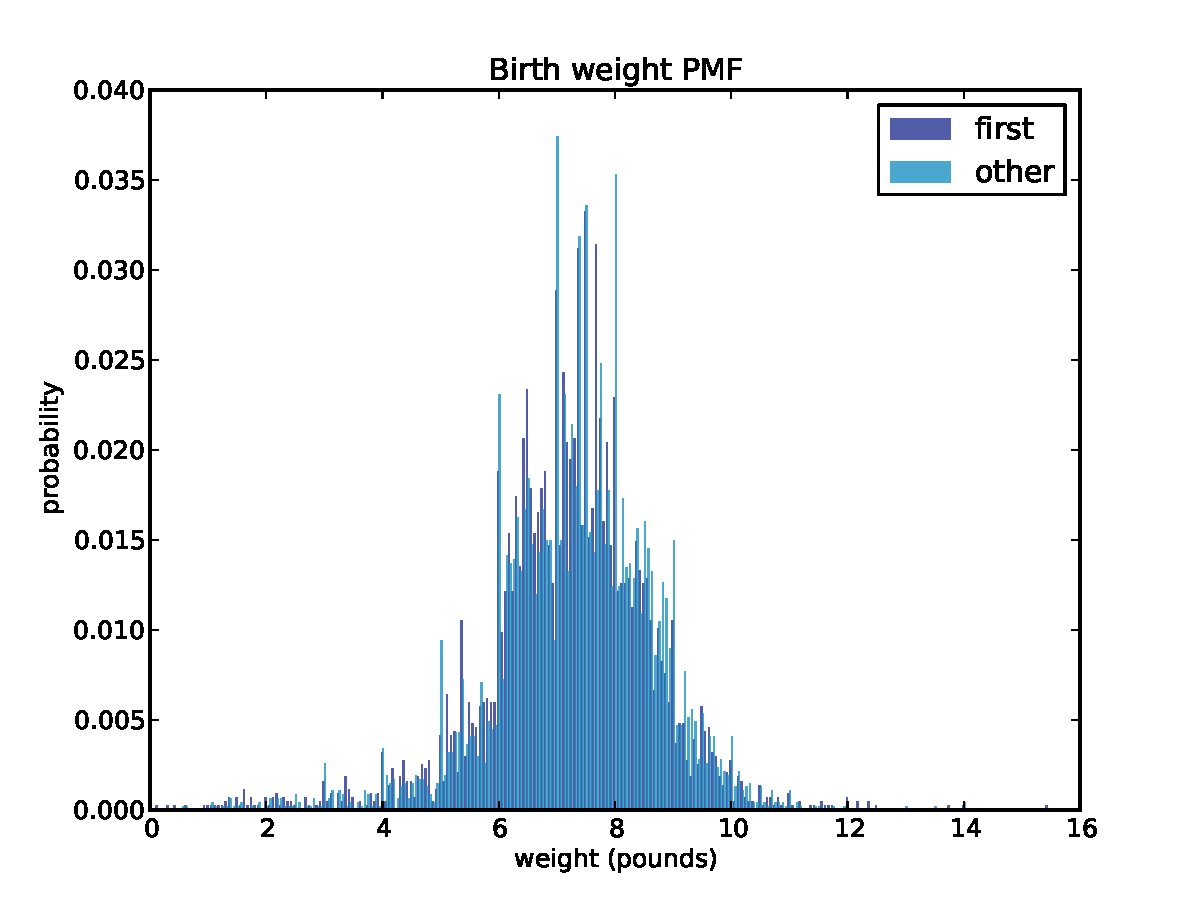
\includegraphics[height=2.5in]{figs/nsfg_birthwgt_pmf.pdf}}
\caption{PMF of birth weights.  This figure shows a limitation
of PMFs: they are hard to compare visually.}
\label{nsfg_birthwgt_pmf}
\end{figure}

Overall, these distributions resemble the bell shape of a normal
distribution, with many values near the mean and a few values much
higher and lower.

But parts of this figure are hard to interpret.  There are many spikes
and valleys, and some apparent differences between the distributions.
It is hard to tell which of these features are meaningful.  Also, it
is hard to see overall patterns; for example, which distribution do
you think has the higher mean?
\index{binning}

These problems can be mitigated by binning the data; that is, dividing
the range of values into non-overlapping intervals and counting the
number of values in each bin.  Binning can be useful, but it is tricky
to get the size of the bins right.  If they are big enough to smooth
out noise, they might also smooth out useful information.

An alternative that avoids these problems is the cumulative
distribution function (CDF), which is the subject of this chapter.
But before I can explain CDFs, I have to explain percentiles.
\index{CDF}


\section{Percentiles}
\index{percentile rank}

If you have taken a standardized test, you probably got your
results in the form of a raw score and a {\bf percentile rank}.
In this context, the percentile rank is the fraction of people who
scored lower than you (or the same).  So if you are ``in the 90th
percentile,'' you did as well as or better than 90\% of the people who
took the exam.

Here's how you could compute the percentile rank of a value,
\verb"your_score", relative to the values in the sequence {\tt
  scores}:
%
\begin{verbatim}
def PercentileRank(scores, your_score):
    count = 0
    for score in scores:
        if score <= your_score:
            count += 1

    percentile_rank = 100.0 * count / len(scores)
    return percentile_rank
\end{verbatim}

As an example, if the
scores in the sequence were 55, 66, 77, 88 and 99, and you got the 88,
then your percentile rank would be {\tt 100 * 4 / 5} which is 80.

If you are given a value, it is easy to find its percentile rank; going
the other way is slightly harder.  If you are given a percentile rank
and you want to find the corresponding value, one option is to
sort the values and search for the one you want:
%
\begin{verbatim}
def Percentile(scores, percentile_rank):
    scores.sort()
    for score in scores:
        if PercentileRank(scores, score) >= percentile_rank:
            return score
\end{verbatim}

The result of this calculation is a {\bf percentile}.  For example,
the 50th percentile is the value with percentile rank 50.  In the
distribution of exam scores, the 50th percentile is 77.
\index{percentile}

This implementation of {\tt Percentile} is not efficient.  A
better approach is to use the percentile rank to compute the index of
the corresponding percentile:

\begin{verbatim}
def Percentile2(scores, percentile_rank):
    scores.sort()
    index = percentile_rank * (len(scores)-1) // 100
    return scores[index]
\end{verbatim}

The difference between ``percentile'' and ``percentile rank'' can
be confusing, and people do not always use the terms precisely.
To summarize, {\tt PercentileRank} takes a value and computes
its percentile rank in a set of values; {\tt Percentile} takes
a percentile rank and computes the corresponding value.
\index{percentile rank}


\section{CDFs}
\index{CDF}

Now that we understand percentiles and percentile ranks,
we are ready to tackle the {\bf cumulative distribution function}
(CDF).  The CDF is the function that maps from a value to its
percentile rank.
\index{cumulative distribution function}
\index{percentile rank}

The CDF is a function of $x$, where $x$ is any value that might appear
in the distribution.  To evaluate $\CDF(x)$ for a particular value of
$x$, we compute the fraction of values in the distribution less
than or equal to $x$.

Here's what that looks like as a function that takes a sequence,
{\tt sample}, and a value, {\tt x}:
%
\begin{verbatim}
def EvalCdf(sample, x):
    count = 0.0
    for value in sample:
        if value <= x:
            count += 1

    prob = count / len(sample)
    return prob
\end{verbatim}

This function is almost identical to {\tt PercentileRank}, except that
the result is a probability in the range 0--1 rather than a
percentile rank in the range 0--100.
\index{sample}

As an example, suppose we collect a sample with the values 
{\tt [1, 2, 2, 3, 5]}.  Here are some values from its CDF:
%
\[ CDF(0) = 0 \]
%
\[ CDF(1) = 0.2\]
%
\[ CDF(2) = 0.6\]
%
\[ CDF(3) = 0.8\]
%
\[ CDF(4) = 0.8\]
%
\[ CDF(5) = 1\]
%
We can evaluate the CDF for any value of $x$, not just
values that appear in the sample.
If $x$ is less than the smallest value in the sample, $\CDF(x)$ is 0.
If $x$ is greater than the largest value, $\CDF(x)$ is 1.

\begin{figure}
% cumulative.py
\centerline{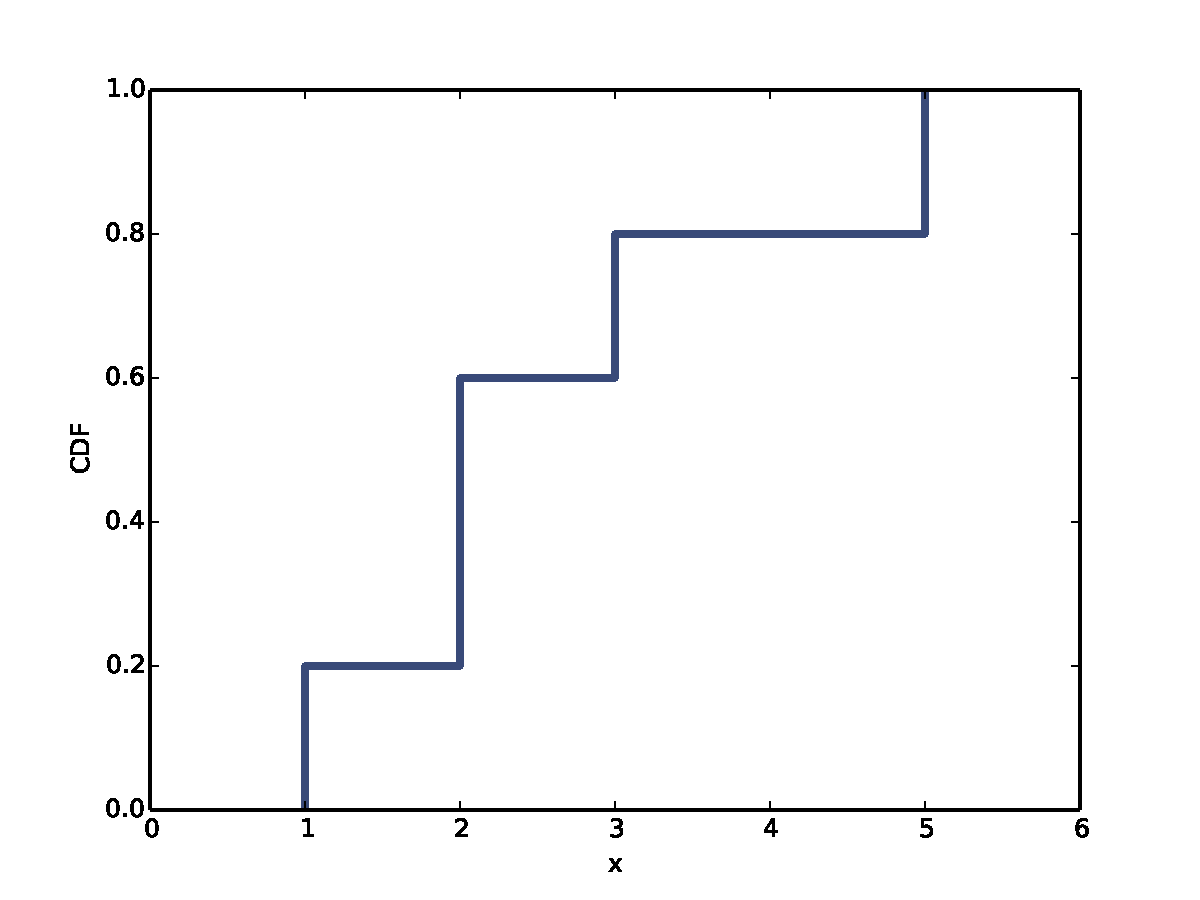
\includegraphics[height=2.5in]{figs/cumulative_example_cdf.pdf}}
\caption{Example of a CDF.}
\label{example_cdf}
\end{figure}

Figure~\ref{example_cdf} is a graphical representation of this CDF.
The CDF of a sample is a step function.
\index{step function}


\section{Representing CDFs}
\index{Cdf}

{\tt thinkstats2} provides a class named Cdf that represents
CDFs.  The fundamental methods Cdf provides are:

\begin{itemize}

\item {\tt Prob(x)}: Given a value {\tt x}, computes the probability
  $p = \CDF(x)$.  The bracket operator is equivalent to {\tt Prob}.
\index{bracket operator}

\item {\tt Value(p)}: Given a probability {\tt p}, computes the
corresponding value, {\tt x}; that is, the {\bf inverse CDF} of {\tt p}.
\index{inverse CDF}
\index{CDF, inverse}

\end{itemize}

\begin{figure}
% cumulative.py
\centerline{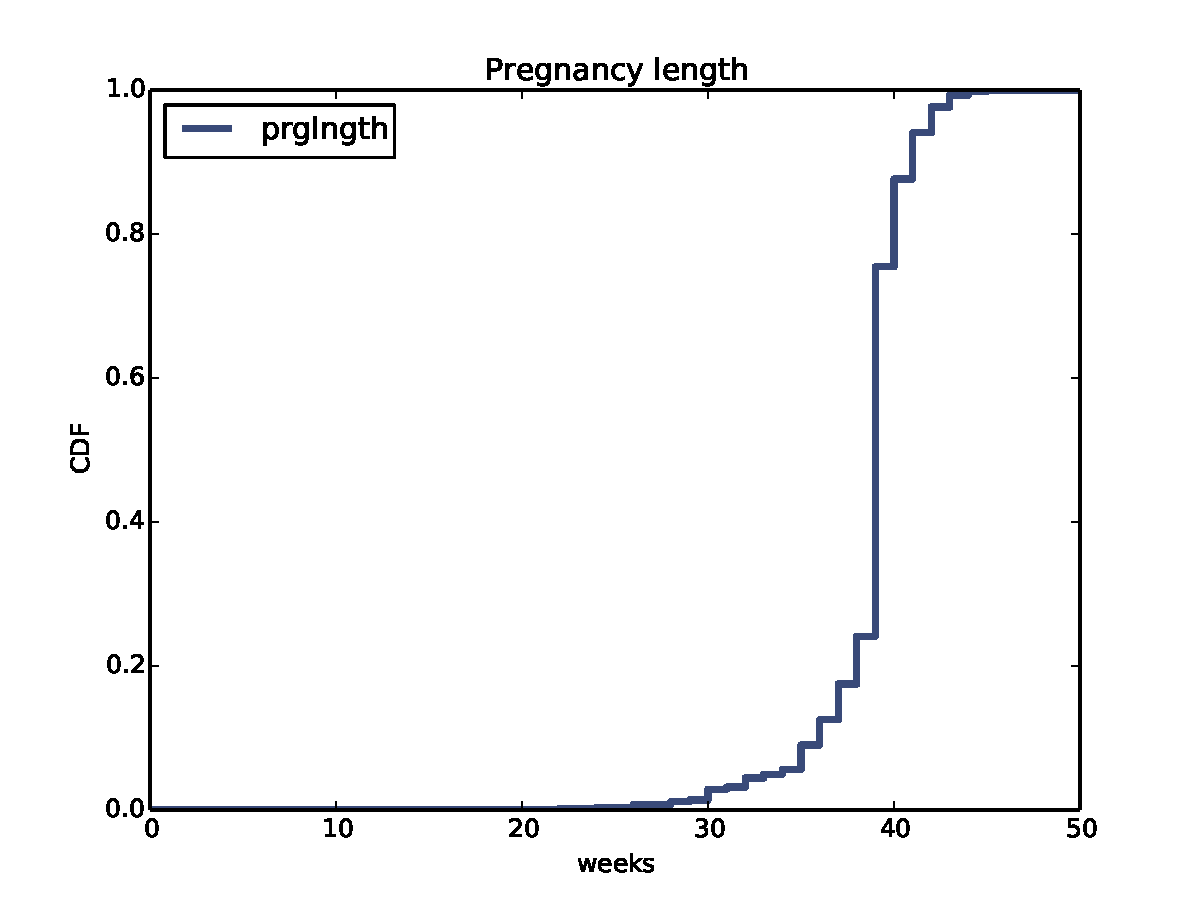
\includegraphics[height=2.5in]{figs/cumulative_prglngth_cdf.pdf}}
\caption{CDF of pregnancy length.}
\label{cumulative_prglngth_cdf}
\end{figure}

The Cdf constructor can take as an argument a list of values,
a pandas Series, a Hist, Pmf, or another Cdf.  The following
code makes a Cdf for the distribution of pregnancy lengths in
the NSFG:
\index{NSFG}
\index{pregnancy length}

\begin{verbatim}
    live, firsts, others = first.MakeFrames()
    cdf = thinkstats2.Cdf(live.prglngth, label='prglngth')
\end{verbatim}

{\tt thinkplot} provides a function named {\tt Cdf} that
plots Cdfs as lines:
\index{thinkplot}

\begin{verbatim}
    thinkplot.Cdf(cdf)
    thinkplot.Show(xlabel='weeks', ylabel='CDF')
\end{verbatim}

Figure~\ref{cumulative_prglngth_cdf} shows the result.  One way to
read a CDF is to look up percentiles.  For example, it looks like
about 10\% of pregnancies are shorter than 36 weeks, and about 90\%
are shorter than 41 weeks.  The CDF also provides a visual
representation of the shape of the distribution.  Common values appear
as steep or vertical sections of the CDF; in this example, the mode at
39 weeks is apparent.  There are few values below 30 weeks, so
the CDF in this range is flat.
\index{CDF, interpreting}

It takes some time to get used to CDFs, but once you
do, I think you will find that they show more information, more
clearly, than PMFs.


\section{Comparing CDFs}
\label{birth_weights}
\index{National Survey of Family Growth}
\index{NSFG}
\index{birth weight}
\index{weight!birth}

CDFs are especially useful for comparing distributions.  For
example, here is the code that plots the CDF of birth
weight for first babies and others.
\index{thinkplot}
\index{distributions, comparing}

\begin{verbatim}
    first_cdf = thinkstats2.Cdf(firsts.totalwgt_lb, label='first')
    other_cdf = thinkstats2.Cdf(others.totalwgt_lb, label='other')

    thinkplot.PrePlot(2)
    thinkplot.Cdfs([first_cdf, other_cdf])
    thinkplot.Show(xlabel='weight (pounds)', ylabel='CDF')
\end{verbatim}

\begin{figure}
% cumulative.py
\centerline{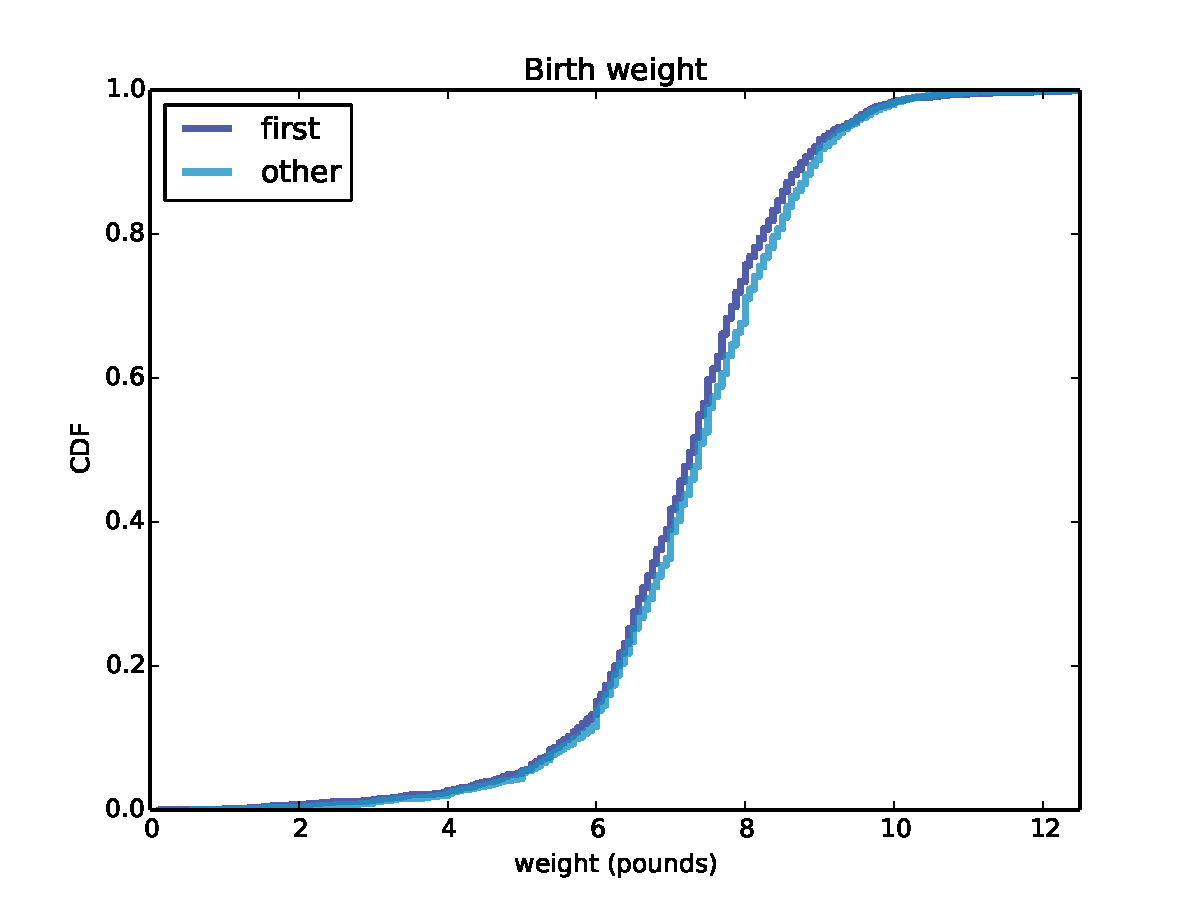
\includegraphics[height=2.5in]{figs/cumulative_birthwgt_cdf.pdf}}
\caption{CDF of birth weights for first babies and others.}
\label{cumulative_birthwgt_cdf}
\end{figure}

Figure~\ref{cumulative_birthwgt_cdf} shows the result.
Compared to Figure~\ref{nsfg_birthwgt_pmf},
this figure makes the shape of the distributions, and the differences
between them, much clearer.  We can see that first babies are slightly
lighter throughout the distribution, with a larger discrepancy above 
the mean.
\index{shape}




\section{Percentile-based statistics}
\index{summary statistic}
\index{interquartile range}
\index{quartile}
\index{percentile}
\index{median}
\index{central tendency}
\index{spread}

Once you have computed a CDF, it is easy to compute percentiles
and percentile ranks.  The Cdf class provides these two methods:
\index{Cdf}
\index{percentile rank}

\begin{itemize}

\item {\tt PercentileRank(x)}: Given a value {\tt x}, computes its
  percentile rank, $100 \cdot \CDF(x)$.

\item {\tt Percentile(p)}: Given a percentile rank {\tt p},
  computes the corresponding value, {\tt x}.  Equivalent to {\tt
    Value(p/100)}.

\end{itemize}

{\tt Percentile} can be used to compute percentile-based summary
statistics.  For example, the 50th percentile is the value that
divides the distribution in half, also known as the {\bf median}.
Like the mean, the median is a measure of the central tendency
of a distribution.

Actually, there are several definitions of ``median,'' each with
different properties.  But {\tt Percentile(50)} is simple and
efficient to compute.

Another percentile-based statistic is the {\bf interquartile range} (IQR),
which is a measure of the spread of a distribution.  The IQR
is the difference between the 75th and 25th percentiles.

More generally, percentiles are often used to summarize the shape
of a distribution.  For example, the distribution of income is
often reported in ``quintiles''; that is, it is split at the
20th, 40th, 60th and 80th percentiles.  Other distributions
are divided into ten ``deciles''.  Statistics like these that represent
equally-spaced points in a CDF are called {\bf quantiles}.
For more, see \url{https://en.wikipedia.org/wiki/Quantile}.
\index{quantile}
\index{quintile}
\index{decile}



\section{Random numbers}
\label{random}
\index{random number}

Suppose we choose a random sample from the population of live
births and look up the percentile rank of their birth weights.
Now suppose we compute the CDF of the percentile ranks.  What do
you think the distribution will look like?
\index{percentile rank}
\index{birth weight}
\index{weight!birth}

Here's how we can compute it.  First, we make the Cdf of
birth weights:
\index{Cdf}

\begin{verbatim}
    weights = live.totalwgt_lb
    cdf = thinkstats2.Cdf(weights, label='totalwgt_lb')
\end{verbatim}

Then we generate a sample and compute the percentile rank of
each value in the sample.

\begin{verbatim}
    sample = np.random.choice(weights, 100, replace=True)
    ranks = [cdf.PercentileRank(x) for x in sample]
\end{verbatim}

{\tt sample}
is a random sample of 100 birth weights, chosen with {\bf replacement};
that is, the same value could be chosen more than once.  {\tt ranks}
is a list of percentile ranks.
\index{replacement}

Finally we make and plot the Cdf of the percentile ranks.
\index{thinkplot}

\begin{verbatim}
    rank_cdf = thinkstats2.Cdf(ranks)
    thinkplot.Cdf(rank_cdf)
    thinkplot.Show(xlabel='percentile rank', ylabel='CDF')
\end{verbatim}

\begin{figure}
% cumulative.py
\centerline{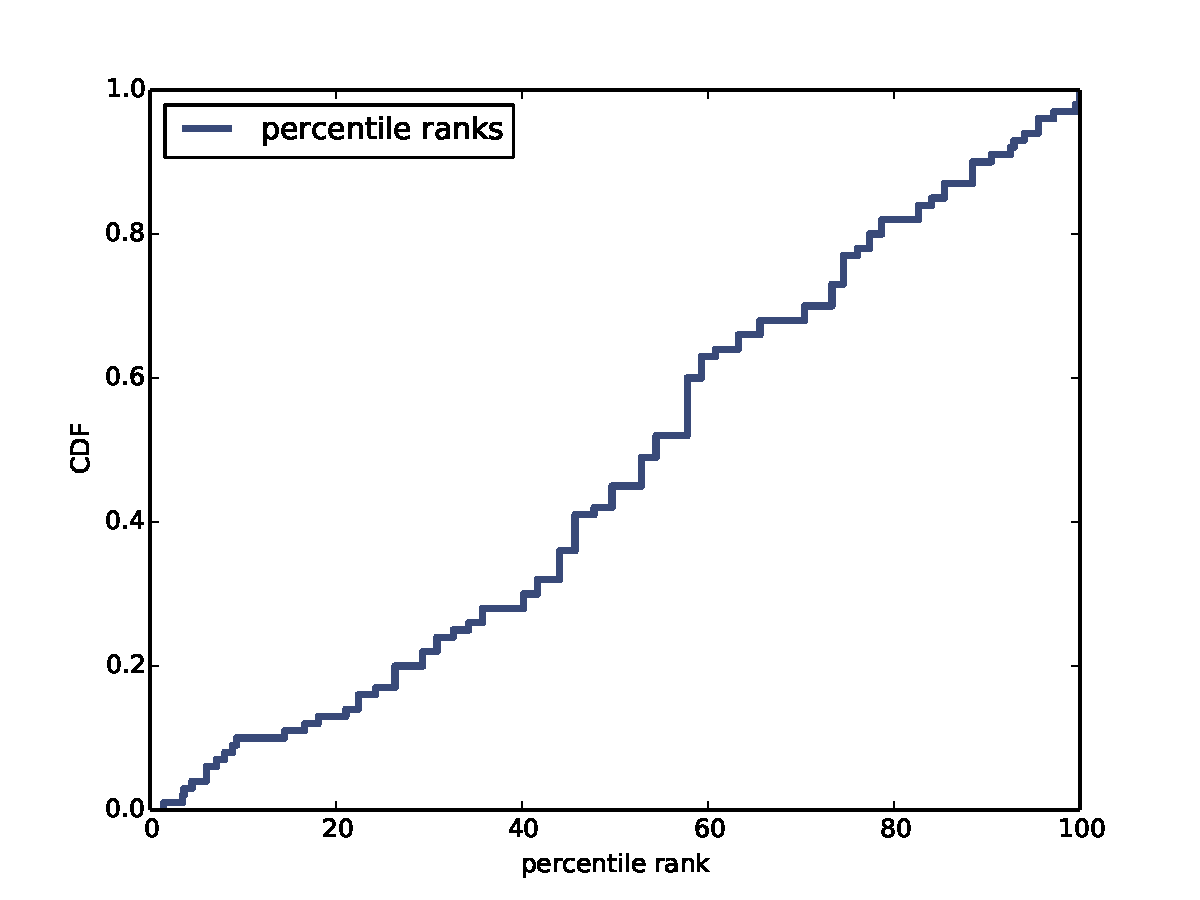
\includegraphics[height=2.5in]{figs/cumulative_random.pdf}}
\caption{CDF of percentile ranks for a random sample of birth weights.}
\label{cumulative_random}
\end{figure}

Figure~\ref{cumulative_random} shows the result.  The CDF is
approximately a straight line, which means that the distribution
is uniform.

That outcome might be non-obvious, but it is a consequence of
the way the CDF is defined.  What this figure shows is that 10\%
of the sample is below the 10th percentile, 20\% is below the
20th percentile, and so on, exactly as we should expect.

So, regardless of the shape of the CDF, the distribution of
percentile ranks is uniform.  This property is useful, because it
is the basis of a simple and efficient algorithm for generating
random numbers with a given CDF.  Here's how:
\index{inverse CDF algorithm}
\index{random number}

\begin{itemize}

\item Choose a percentile rank uniformly from the range 0--100.

\item Use {\tt Cdf.Percentile} to find the value in the distribution
that corresponds to the percentile rank you chose.
\index{Cdf}

\end{itemize}

Cdf provides an implementation of this algorithm, called
{\tt Random}:

\begin{verbatim}
# class Cdf:
    def Random(self):
        return self.Percentile(random.uniform(0, 100))
\end{verbatim}

Cdf also provides {\tt Sample}, which takes an integer,
{\tt n}, and returns a list of {\tt n} values chosen at random
from the Cdf.


\section{Comparing percentile ranks}

Percentile ranks are useful for comparing measurements across
different groups.  For example, people who compete in foot races are
usually grouped by age and gender.  To compare people in different
age groups, you can convert race times to percentile ranks.
\index{percentile rank}

A few years ago I ran the James Joyce Ramble 10K in
Dedham MA; I finished in 42:44, which was 97th in a field of 1633.  I beat or
tied 1537 runners out of 1633, so my percentile rank in the field is
94\%.  \index{James Joyce Ramble} \index{race time}

More generally, given position and field size, we can compute
percentile rank:
\index{field size}

\begin{verbatim}
def PositionToPercentile(position, field_size):
    beat = field_size - position + 1
    percentile = 100.0 * beat / field_size
    return percentile
\end{verbatim}

In my age group, denoted M4049 for ``male between 40 and 49 years of
age'', I came in 26th out of 256.  So my percentile rank in my age
group was 90\%.
\index{age group}

If I am still running in 10 years (and I hope I am), I will be in
the M5059 division.  Assuming that my percentile rank in my division
is the same, how much slower should I expect to be?

I can answer that question by converting my percentile rank in M4049
to a position in M5059.  Here's the code:

\begin{verbatim}
def PercentileToPosition(percentile, field_size):
    beat = percentile * field_size / 100.0
    position = field_size - beat + 1
    return position
\end{verbatim}

There were 171 people in M5059, so I would have to come in between
17th and 18th place to have the same percentile rank.  The finishing
time of the 17th runner in M5059 was 46:05, so that's the time I will
have to beat to maintain my percentile rank.


\section{Exercises}

For the following exercises, you can start with \verb"chap04ex.ipynb".
My solution is in \verb"chap04soln.ipynb".

\begin{exercise}
How much did you weigh at birth?  If you don't know, call your mother
or someone else who knows.  Using the NSFG data (all live births),
compute the distribution of birth weights and use it to find your
percentile rank.  If you were a first baby, find your percentile rank
in the distribution for first babies.  Otherwise use the distribution
for others.  If you are in the 90th percentile or higher, call your
mother back and apologize.
\index{birth weight}
\index{weight!birth}

\end{exercise}

\begin{exercise}
The numbers generated by {\tt random.random} are supposed to be
uniform between 0 and 1; that is, every value in the range
should have the same probability.

Generate 1000 numbers from {\tt random.random} and plot their
PMF and CDF.  Is the distribution uniform?
\index{uniform distribution}
\index{distribution!uniform}
\index{random number}

\end{exercise}


\section{Glossary}

\begin{itemize}

\item percentile rank: The percentage of values in a distribution that are
less than or equal to a given value.
\index{percentile rank}

\item percentile: The value associated with a given percentile rank.
\index{percentile}

\item cumulative distribution function (CDF): A function that maps
  from values to their cumulative probabilities.  $\CDF(x)$ is the
  fraction of the sample less than or equal to $x$.  \index{CDF}
\index{cumulative probability}

\item inverse CDF: A function that maps from a cumulative probability,
  $p$, to the corresponding value.
\index{inverse CDF}
\index{CDF, inverse}

\item median: The 50th percentile, often used as a measure of central
  tendency.  \index{median}

\item interquartile range: The difference between
the 75th and 25th percentiles, used as a measure of spread.
\index{interquartile range}

\item quantile: A sequence of values that correspond to equally spaced
percentile ranks; for example, the quartiles of a distribution are
the 25th, 50th and 75th percentiles.
\index{quantile}

\item replacement: A property of a sampling process. ``With replacement''
means that the same value can be chosen more than once; ``without
replacement'' means that once a value is chosen, it is removed from
the population.
\index{replacement}

\end{itemize}


\chapter{Modeling distributions}
\label{modeling}

The distributions we have used so far are called {\bf empirical
  distributions} because they are based on empirical observations,
which are necessarily finite samples.
\index{analytic distribution}
\index{distribution!analytic}
\index{empirical distribution}
\index{distribution!empirical}

The alternative is an {\bf analytic distribution}, which is
characterized by a CDF that is a mathematical function.
Analytic distributions can be used to model empirical distributions.
In this context, a {\bf model} is a simplification that leaves out
unneeded details.  This chapter presents common analytic distributions
and uses them to model data from a variety of sources.
\index{model}

The code for this chapter is in {\tt analytic.py}.  For information
about downloading and working with this code, see Section~\ref{code}.



\section{The exponential distribution}
\label{exponential}
\index{exponential distribution}
\index{distribution!exponential}

\begin{figure}
% analytic.py
\centerline{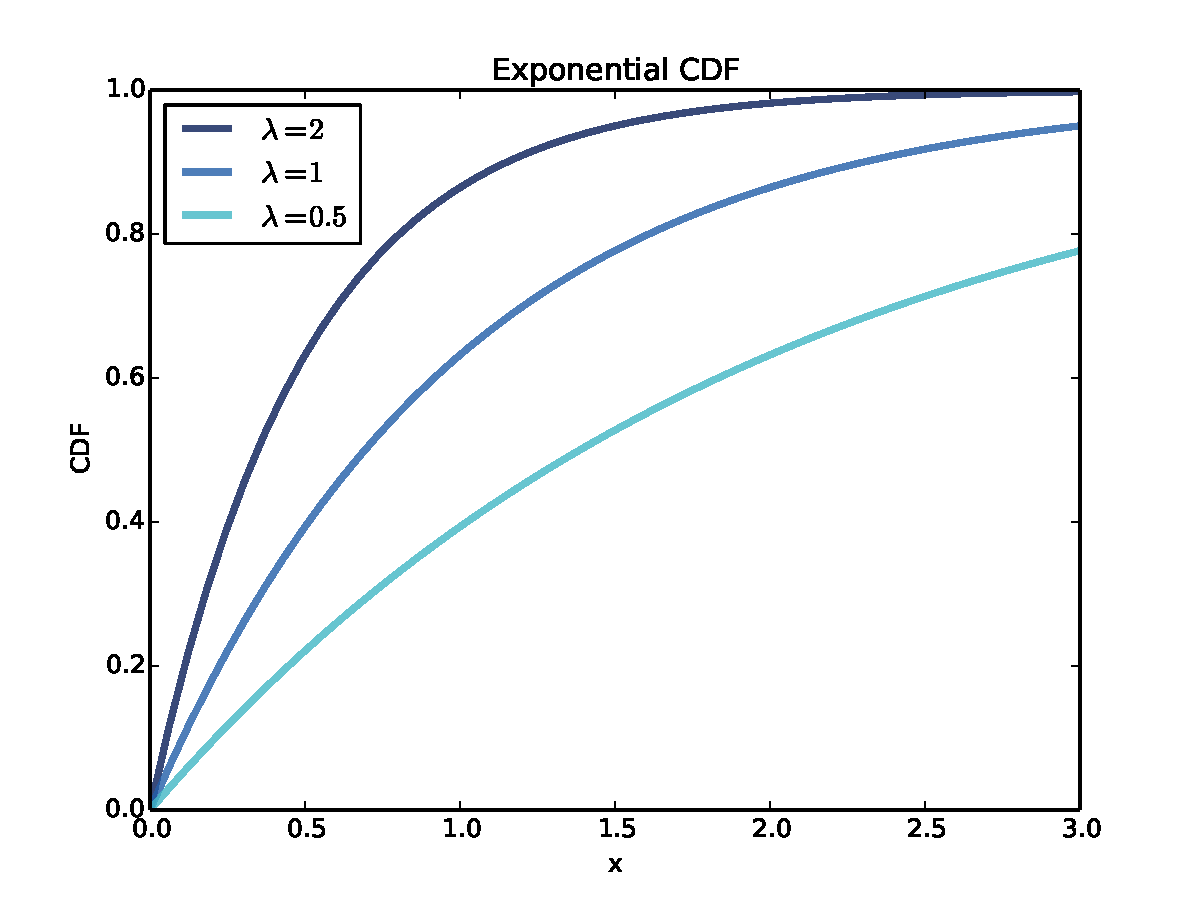
\includegraphics[height=2.5in]{figs/analytic_expo_cdf.pdf}}
\caption{CDFs of exponential distributions with various parameters.}
\label{analytic_expo_cdf}
\end{figure}

I'll start with the {\bf exponential distribution} because it is
relatively simple.  The CDF of the exponential distribution is
%
\[ \CDF(x) = 1 - e^{-\lambda x} \]
%
The parameter, $\lambda$, determines the shape of the distribution.
Figure~\ref{analytic_expo_cdf} shows what this CDF looks like with
$\lambda = $ 0.5, 1, and 2.
  \index{parameter}

In the real world, exponential distributions
come up when we look at a series of events and measure the
times between events, called {\bf interarrival times}.
If the events are equally likely to occur at any time, the distribution
of interarrival times tends to look like an exponential distribution.
\index{interarrival time}

As an example, we will look at the interarrival time of births.
On December 18, 1997, 44 babies were born in a hospital in Brisbane,
Australia.\footnote{This example is based on information and data from
  Dunn, ``A Simple Dataset for Demonstrating Common Distributions,''
  Journal of Statistics Education v.7, n.3 (1999).}  The time of
birth for all 44 babies was reported in the local paper; the
complete dataset is in a file called {\tt babyboom.dat}, in the
{\tt ThinkStats2} repository.
\index{birth time}
\index{Australia} \index{Brisbane}

\begin{verbatim}
    df = ReadBabyBoom()
    diffs = df.minutes.diff()
    cdf = thinkstats2.Cdf(diffs, label='actual')

    thinkplot.Cdf(cdf)
    thinkplot.Show(xlabel='minutes', ylabel='CDF')
\end{verbatim}

{\tt ReadBabyBoom} reads the data file and returns a DataFrame
with columns {\tt time}, {\tt sex}, \verb"weight_g", and {\tt minutes},
where {\tt minutes} is time of birth converted to minutes since
midnight.
\index{DataFrame}
\index{thinkplot}

\begin{figure}
% analytic.py
\centerline{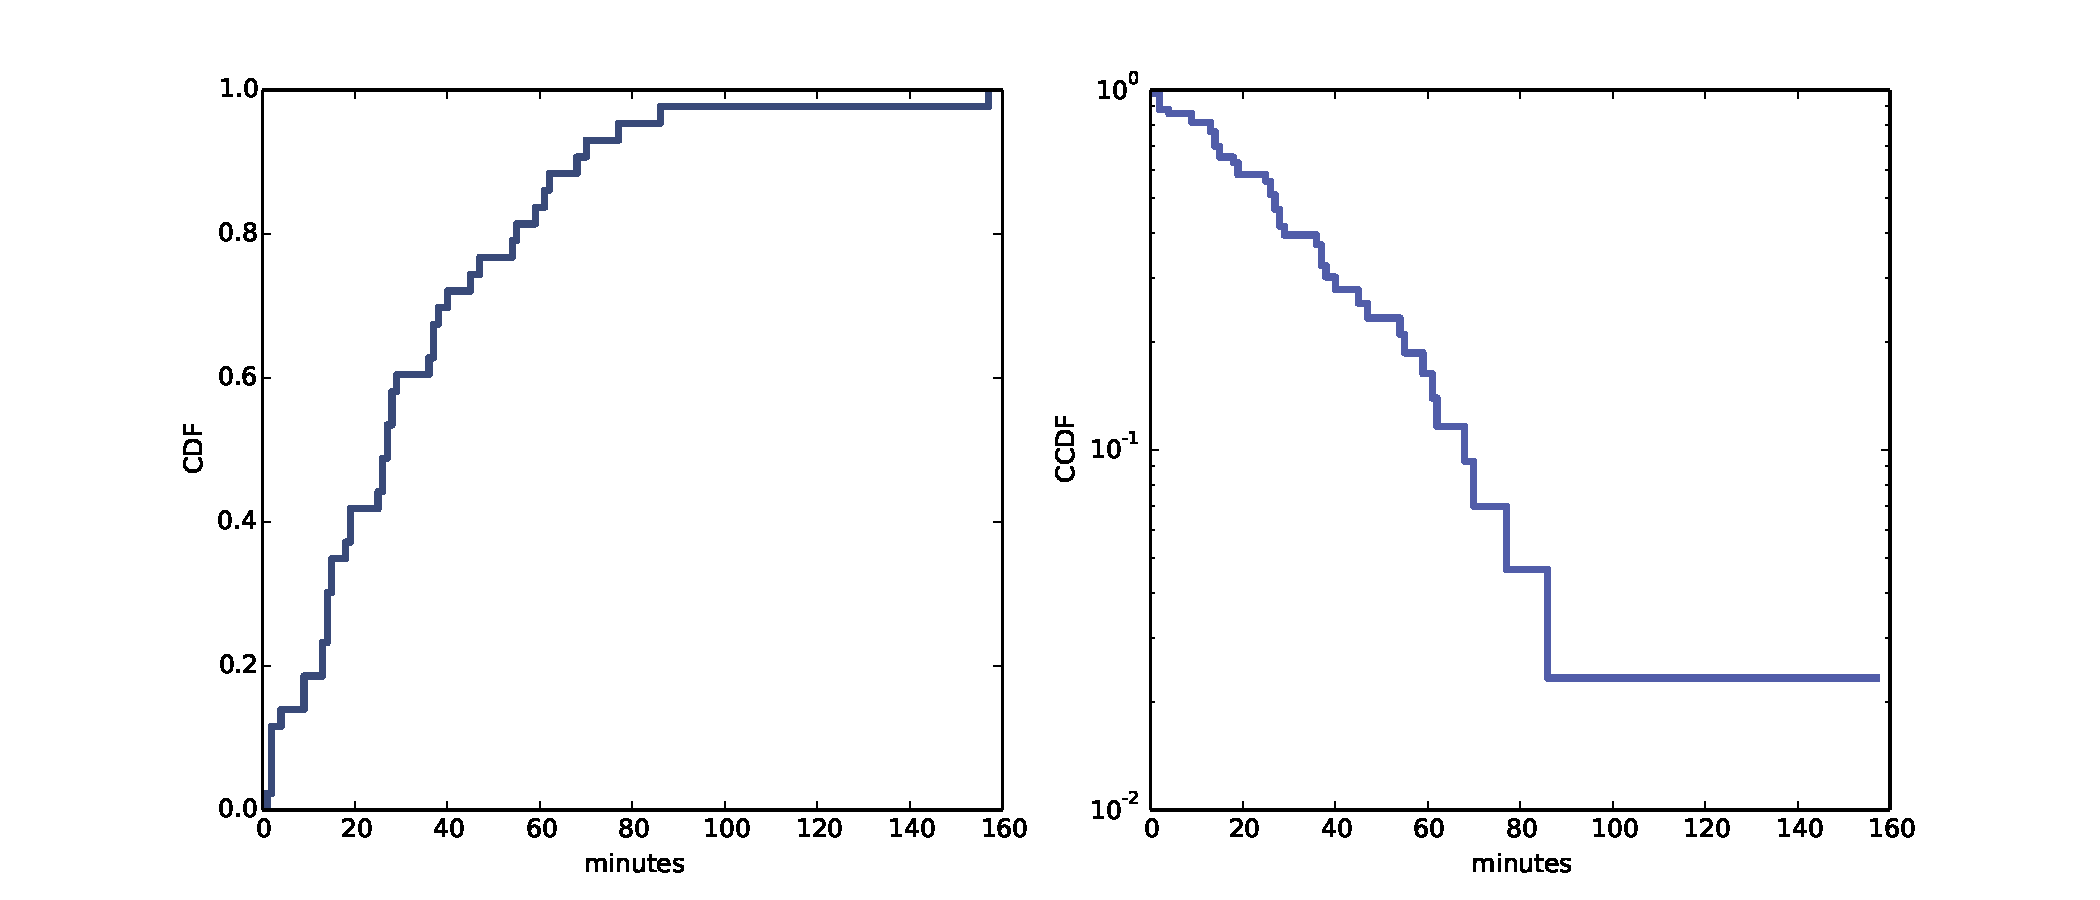
\includegraphics[height=2.5in]{figs/analytic_interarrivals.pdf}}
\caption{CDF of interarrival times (left) and CCDF on a log-y scale (right).}
\label{analytic_interarrival_cdf}
\end{figure}

%\begin{figure}
% analytic.py
%\centerline{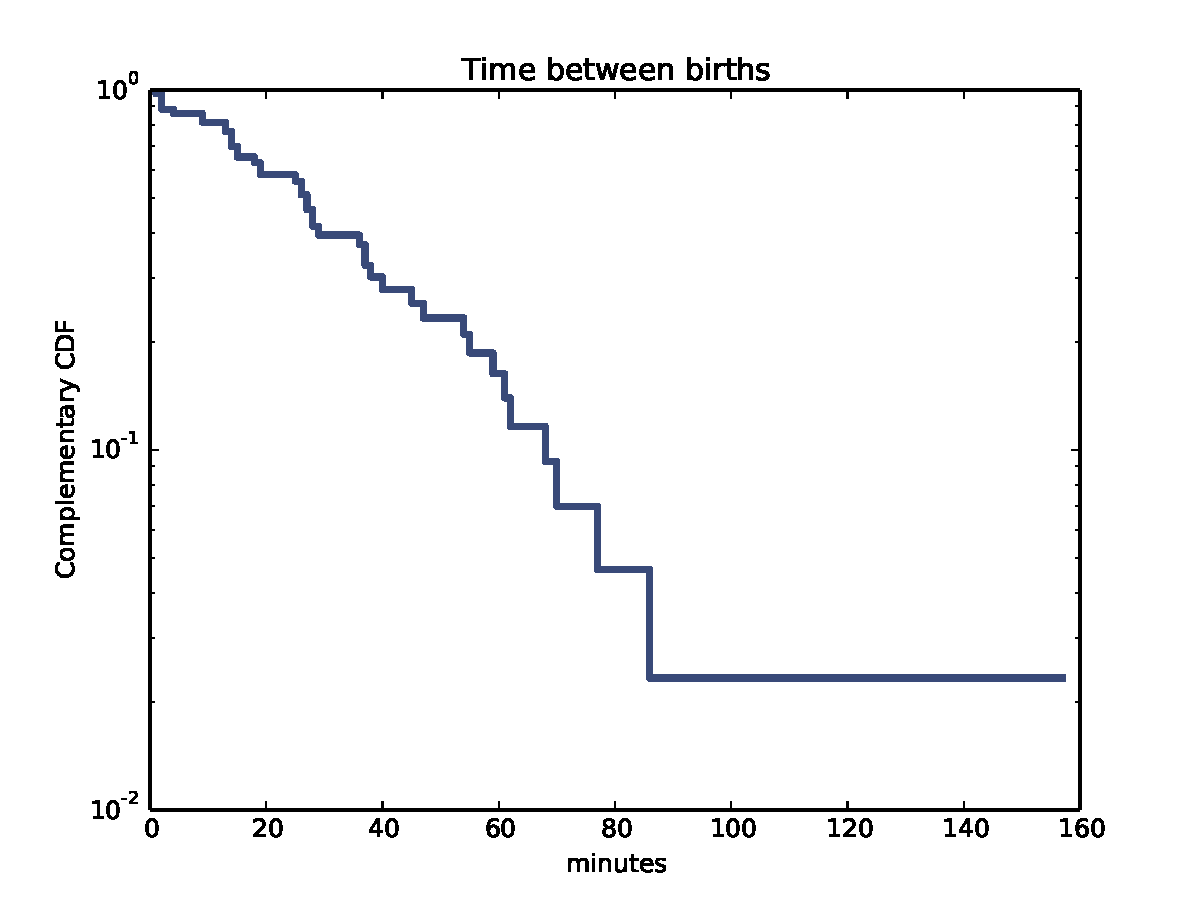
\includegraphics[height=2.5in]{figs/analytic_interarrivals_logy.pdf}}
%\caption{CCDF of interarrival times.}
%\label{analytic_interarrival_ccdf}
%\end{figure}

{\tt diffs} is the difference between consecutive birth times, and
{\tt cdf} is the distribution of these interarrival times.
Figure~\ref{analytic_interarrival_cdf} (left) shows the CDF.  It seems
to have the general shape of an exponential distribution, but how can
we tell?

One way is to plot the {\bf complementary CDF}, which is $1 - \CDF(x)$,
on a log-y scale.  For data from an exponential distribution, the
result is a straight line.  Let's see why that works.
\index{complementary CDF} \index{CDF!complementary} \index{CCDF}

If you plot the complementary CDF (CCDF) of a dataset that you think is
exponential, you expect to see a function like:
%
\[ y \approx e^{-\lambda x} \]
%
Taking the log of both sides yields:
%
\[ \log y \approx -\lambda x\]
%
So on a log-y scale the CCDF is a straight line
with slope $-\lambda$.  Here's how we can generate a plot like that:
\index{logarithmic scale}
\index{complementary CDF}
\index{CDF!complementary}
\index{CCDF}


\begin{verbatim}
    thinkplot.Cdf(cdf, complement=True)
    thinkplot.Show(xlabel='minutes',
                   ylabel='CCDF',
                   yscale='log')
\end{verbatim}

With the argument {\tt complement=True}, {\tt thinkplot.Cdf} computes
the complementary CDF before plotting.  And with {\tt yscale='log'},
{\tt thinkplot.Show} sets the {\tt y} axis to a logarithmic scale.
\index{thinkplot}
\index{Cdf}

Figure~\ref{analytic_interarrival_cdf} (right) shows the result.  It is not
exactly straight, which indicates that the exponential distribution is
not a perfect model for this data.  Most likely the underlying
assumption---that a birth is equally likely at any time of day---is
not exactly true.  Nevertheless, it might be reasonable to model this
dataset with an exponential distribution.  With that simplification, we can
summarize the distribution with a single parameter.
\index{model}

The parameter, $\lambda$, can be interpreted as a rate; that is, the
number of events that occur, on average, in a unit of time.  In this
example, 44 babies are born in 24 hours, so the rate is $\lambda =
0.0306$ births per minute.  The mean of an exponential distribution is
$1/\lambda$, so the mean time between births is 32.7 minutes.


\section{The normal distribution}
\label{normal}

The {\bf normal distribution}, also called Gaussian, is commonly
used because it describes many phenomena, at least approximately.
It turns out that there is a good reason for its ubiquity, which we
will get to in Section~\ref{CLT}.
\index{CDF}
\index{parameter}
\index{mean}
\index{standard deviation}
\index{normal distribution}
\index{distribution!normal}
\index{Gaussian distribution}
\index{distribution!Gaussian}

%
%\[ \CDF(z) = \frac{1}{\sqrt{2 \pi}} \int_{-\infty}^z e^{-t^2/2} dt \]
%

\begin{figure}
% analytic.py
\centerline{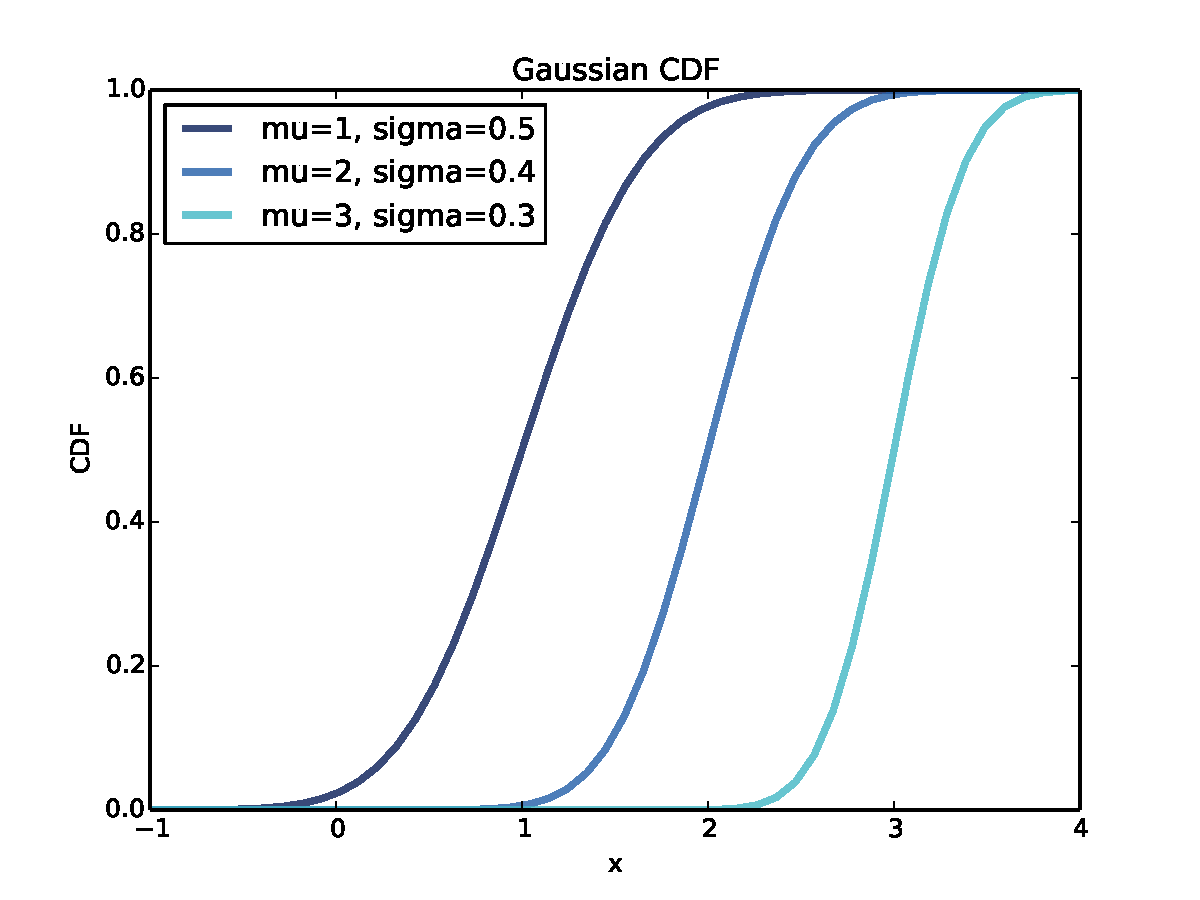
\includegraphics[height=2.5in]{figs/analytic_gaussian_cdf.pdf}}
\caption{CDF of normal distributions with a range of parameters.}
\label{analytic_gaussian_cdf}
\end{figure}

The normal distribution is characterized by two parameters: the mean,
$\mu$, and standard deviation $\sigma$.  The normal distribution with
$\mu=0$ and $\sigma=1$ is called the {\bf standard normal
  distribution}.  Its CDF is defined by an integral that does not have
a closed form solution, but there are algorithms that evaluate it
efficiently.  One of them is provided by SciPy: {\tt scipy.stats.norm}
is an object that represents a normal distribution; it provides a
method, {\tt cdf}, that evaluates the standard normal CDF:
\index{SciPy}
\index{closed form}

\begin{verbatim}
>>> import scipy.stats
>>> scipy.stats.norm.cdf(0)
0.5
\end{verbatim}

This result is correct: the median of the standard normal distribution
is 0 (the same as the mean), and half of the values fall below the
median, so $\CDF(0)$ is 0.5.

{\tt norm.cdf} takes optional parameters: {\tt loc}, which
specifies the mean, and {\tt scale}, which specifies the
standard deviation.

{\tt thinkstats2} makes this function a little easier to use
by providing {\tt EvalNormalCdf}, which takes parameters {\tt mu}
and {\tt sigma} and evaluates the CDF at {\tt x}:
\index{normal distribution}

\begin{verbatim}
def EvalNormalCdf(x, mu=0, sigma=1):
    return scipy.stats.norm.cdf(x, loc=mu, scale=sigma)
\end{verbatim}

Figure~\ref{analytic_gaussian_cdf} shows CDFs for normal
distributions with a range of parameters.  The sigmoid shape of these
curves is a recognizable characteristic of a normal distribution.

In the previous chapter we looked at the distribution of birth
weights in the NSFG.  Figure~\ref{analytic_birthwgt_model} shows the
empirical CDF of weights for all live births and the CDF of
a normal distribution with the same mean and variance.
\index{National Survey of Family Growth}
\index{NSFG}
\index{birth weight}
\index{weight!birth}

\begin{figure}
% analytic.py
\centerline{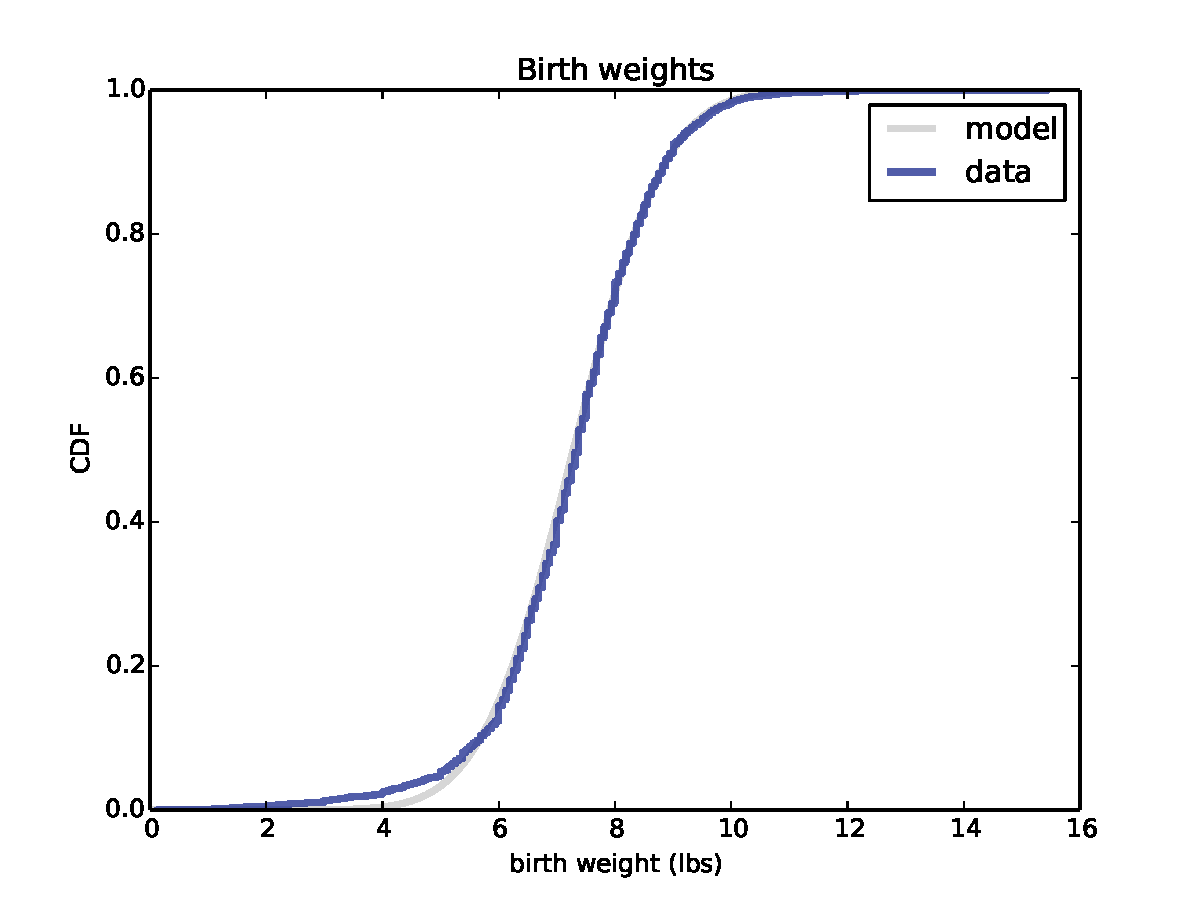
\includegraphics[height=2.5in]{figs/analytic_birthwgt_model.pdf}}
\caption{CDF of birth weights with a normal model.}
\label{analytic_birthwgt_model}
\end{figure}

The normal distribution is a good model for this dataset, so
if we summarize the distribution with the parameters
$\mu = 7.28$ and $\sigma = 1.24$, the resulting error
(difference between the model and the data) is small.
\index{model}
\index{percentile}

Below the 10th percentile there is a discrepancy between the data
and the model; there are more light babies than we would expect in
a normal distribution.  If we are specifically interested in preterm
babies, it would be important to get this part of the distribution
right, so it might not be appropriate to use the normal
model.


\section{Normal probability plot}

For the exponential distribution, and a few others, there are
simple transformations we can use to test whether an analytic
distribution is a good model for a dataset.
\index{exponential distribution}
\index{distribution!exponential}
\index{model}

For the normal distribution there is no such transformation, but there
is an alternative called a {\bf normal probability plot}.  There
are two ways to generate a normal probability plot: the hard way
and the easy way.  If you are interested in the hard way, you can
read about it at \url{https://en.wikipedia.org/wiki/Normal_probability_plot}.
Here's the easy way:
\index{normal probability plot}
\index{plot!normal probability}
\index{normal distribution}
\index{distribution!normal}
\index{Gaussian distribution}
\index{distribution!Gaussian}

\begin{enumerate}

\item Sort the values in the sample.

\item From a standard normal distribution ($\mu=0$ and $\sigma=1$),
generate a random sample with the same size as the sample, and sort it.
\index{random number}

\item Plot the sorted values from the sample versus the random values.

\end{enumerate}

If the distribution of the sample is approximately normal, the result
is a straight line with intercept {\tt mu} and slope {\tt sigma}.
{\tt thinkstats2} provides {\tt NormalProbability}, which takes a
sample and returns two NumPy arrays:
\index{NumPy}

\begin{verbatim}
xs, ys = thinkstats2.NormalProbability(sample)
\end{verbatim}

\begin{figure}
% analytic.py
\centerline{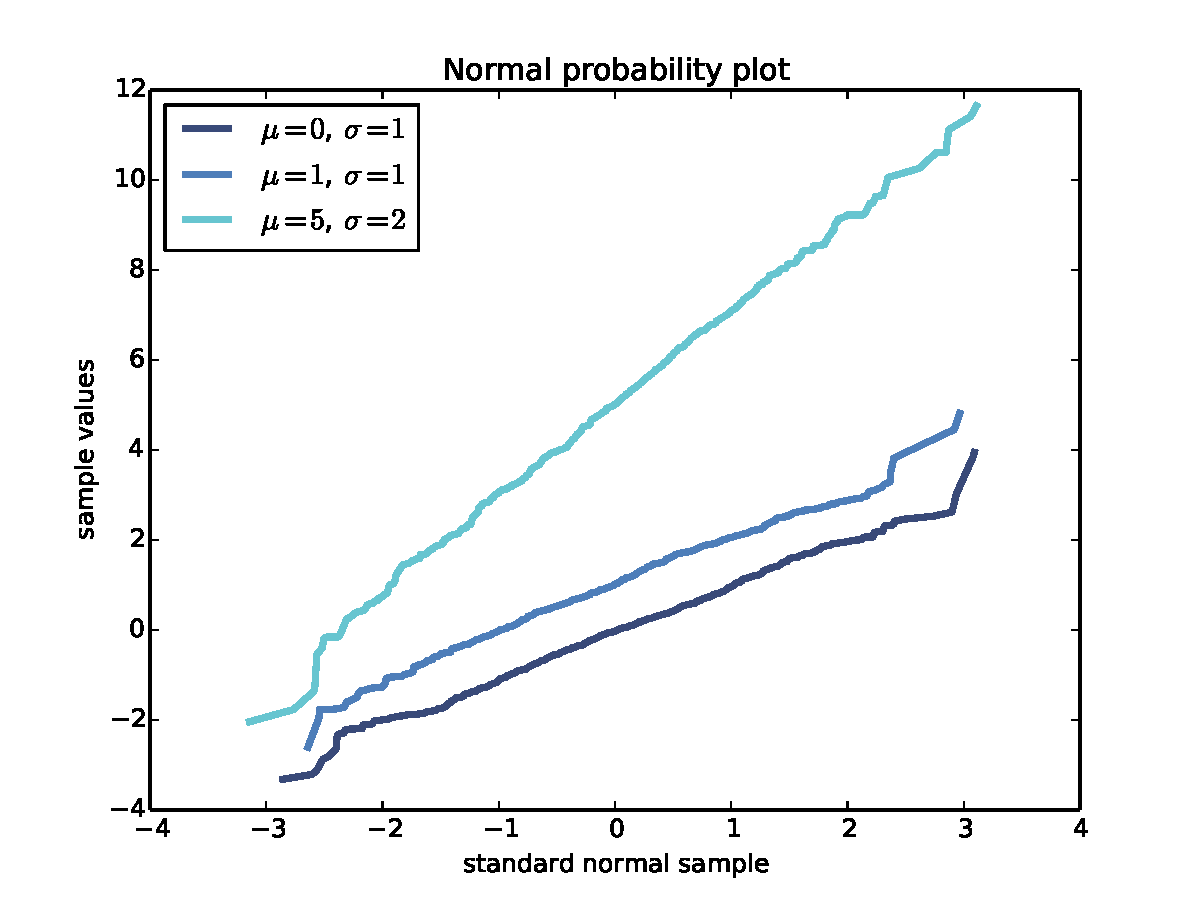
\includegraphics[height=2.5in]{figs/analytic_normal_prob_example.pdf}}
\caption{Normal probability plot for random samples from normal distributions.}
\label{analytic_normal_prob_example}
\end{figure}

{\tt ys} contains the sorted values from {\tt sample}; {\tt xs}
contains the random values from the standard normal distribution.

To test {\tt NormalProbability} I generated some fake samples that
were actually drawn from normal distributions with various parameters.
Figure~\ref{analytic_normal_prob_example} shows the results.
The lines are approximately straight, with values in the tails
deviating more than values near the mean.

Now let's try it with real data.  Here's code to generate
a normal probability plot for the birth weight data from the
previous section.  It plots a gray line that represents the model
and a blue line that represents the data.
\index{birth weight}
\index{weight!birth}

\begin{verbatim}
def MakeNormalPlot(weights):
    mean = weights.mean()
    std = weights.std()

    xs = [-4, 4]
    fxs, fys = thinkstats2.FitLine(xs, inter=mean, slope=std)
    thinkplot.Plot(fxs, fys, color='gray', label='model')

    xs, ys = thinkstats2.NormalProbability(weights)
    thinkplot.Plot(xs, ys, label='birth weights')
\end{verbatim}

{\tt weights} is a pandas Series of birth weights;
{\tt mean} and {\tt std} are the mean and standard deviation.
\index{pandas}
\index{Series}
\index{thinkplot}
\index{standard deviation}

{\tt FitLine} takes a sequence of {\tt xs}, an intercept, and a
slope; it returns {\tt xs} and {\tt ys} that represent a line
with the given parameters, evaluated at the values in {\tt xs}.

{\tt NormalProbability} returns {\tt xs} and {\tt ys} that
contain values from the standard normal distribution and values
from {\tt weights}.  If the distribution of weights is normal,
the data should match the model.
\index{model}

\begin{figure}
% analytic.py
\centerline{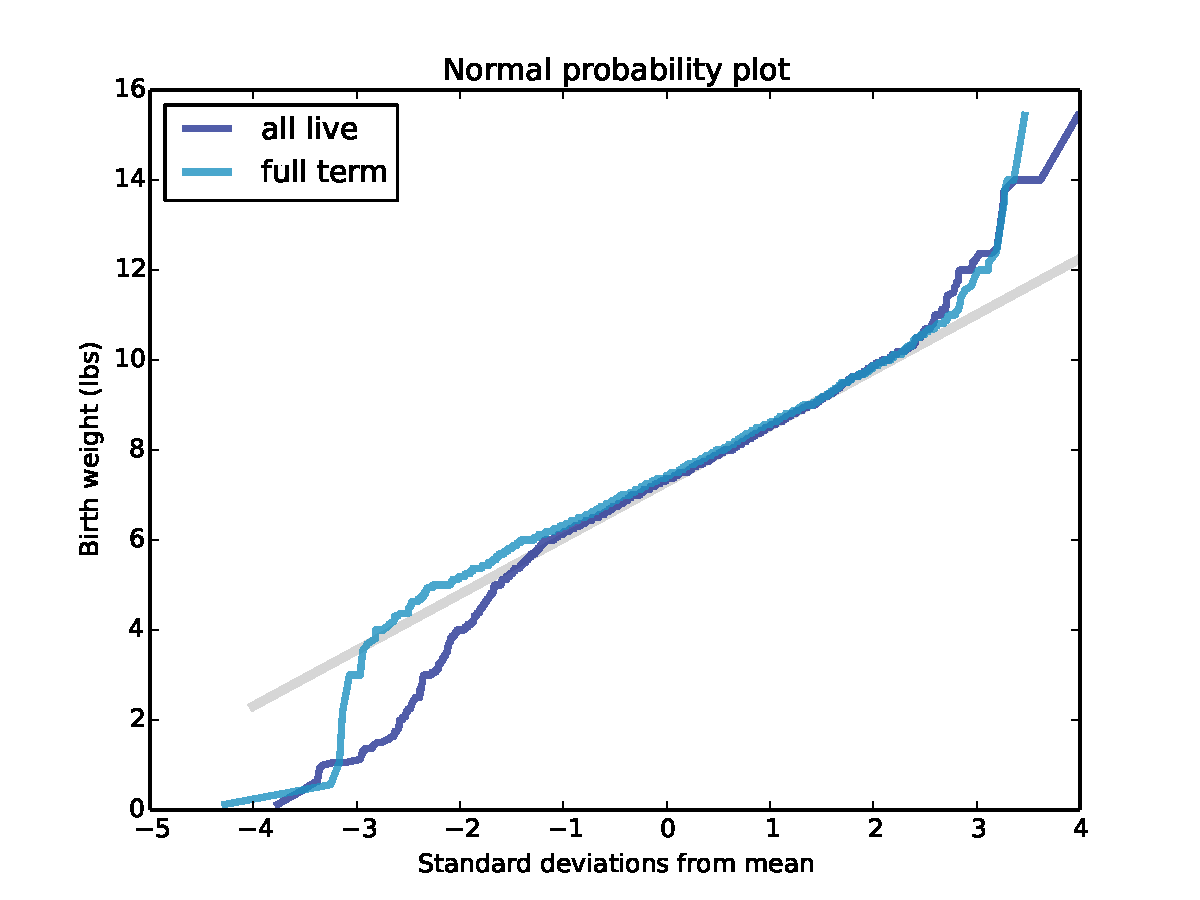
\includegraphics[height=2.5in]{figs/analytic_birthwgt_normal.pdf}}
\caption{Normal probability plot of birth weights.}
\label{analytic_birthwgt_normal}
\end{figure}

Figure~\ref{analytic_birthwgt_normal} shows the results for
all live births, and also for full term births (pregnancy length greater
than 36 weeks).  Both curves match the model near the mean and
deviate in the tails.  The heaviest babies are heavier than what
the model expects, and the lightest babies are lighter.
\index{pregnancy length}

When we select only full term births, we remove some of the lightest
weights, which reduces the discrepancy in the lower tail of the
distribution.

This plot suggests that the normal model describes the distribution
well within a few standard deviations from the mean, but not in the
tails.  Whether it is good enough for practical purposes depends
on the purposes.
\index{model}
\index{birth weight}
\index{weight!birth}
\index{standard deviation}


\section{The lognormal distribution}
\label{brfss}
\label{lognormal}

If the logarithms of a set of values have a normal distribution, the
values have a {\bf lognormal distribution}.  The CDF of the lognormal
distribution is the same as the CDF of the normal distribution,
with $\log x$ substituted for $x$.
%
\[ CDF_{lognormal}(x) = CDF_{normal}(\log x)\]
%
The parameters of the lognormal distribution are usually denoted
$\mu$ and $\sigma$.  But remember that these parameters are {\em not}
the mean and standard deviation; the mean of a lognormal distribution
is $\exp(\mu +\sigma^2/2)$ and the standard deviation is
ugly (see \url{http://wikipedia.org/wiki/Log-normal_distribution}).
\index{parameter} \index{weight!adult} \index{adult weight}
\index{lognormal distribution}
\index{distribution!lognormal}
\index{CDF}

\begin{figure}
% brfss.py
\centerline{
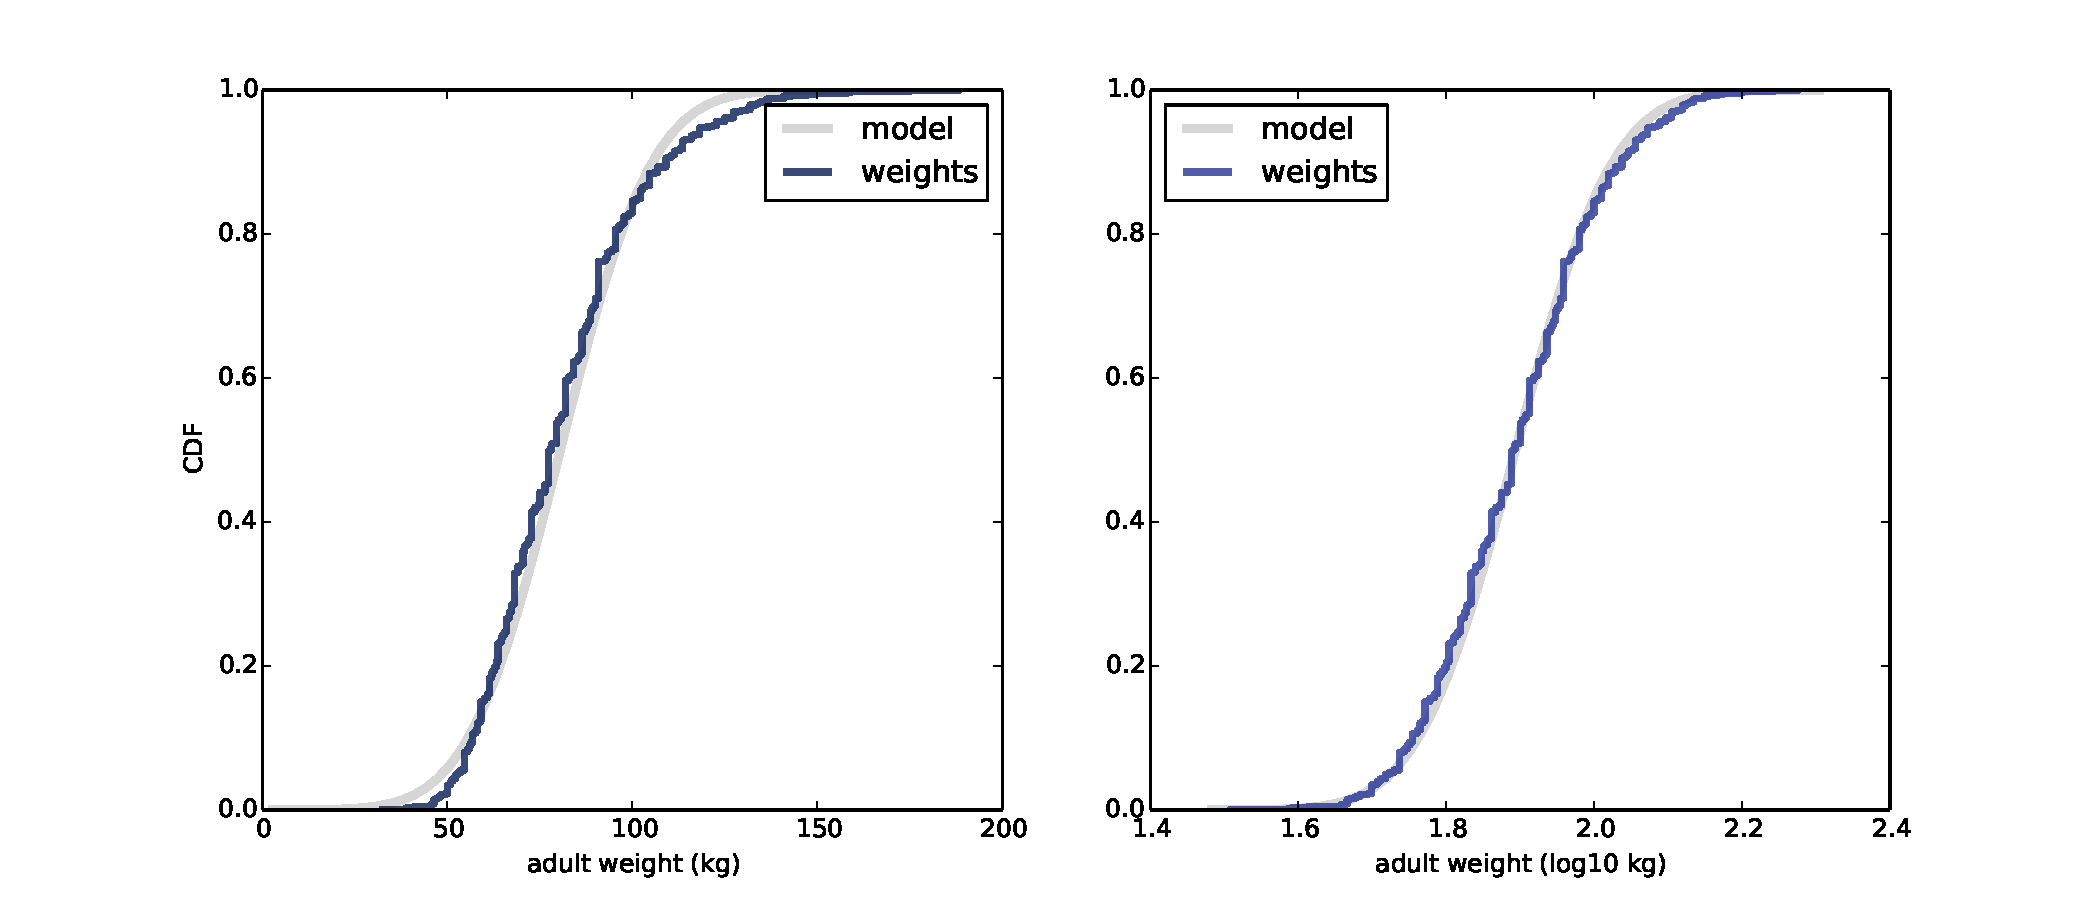
\includegraphics[height=2.5in]{figs/brfss_weight.pdf}}
\caption{CDF of adult weights on a linear scale (left) and
log scale (right).}
\label{brfss_weight}
\end{figure}

If a sample is approximately lognormal and you plot its CDF on a
log-x scale, it will have the characteristic shape of a normal
distribution.  To test how well the sample fits a lognormal model, you
can make a normal probability plot using the log of the values
in the sample.
\index{normal probability plot}
\index{model}

As an example, let's look at the distribution of adult weights, which
is approximately lognormal.\footnote{I was tipped off to this
  possibility by a comment (without citation) at
  \url{http://mathworld.wolfram.com/LogNormalDistribution.html}.
  Subsequently I found a paper that proposes the log transform and
  suggests a cause: Penman and Johnson, ``The Changing Shape of the
  Body Mass Index Distribution Curve in the Population,'' Preventing
  Chronic Disease, 2006 July; 3(3): A74.  Online at
  \url{http://www.ncbi.nlm.nih.gov/pmc/articles/PMC1636707}.}

The National Center for Chronic Disease
Prevention and Health Promotion conducts an annual survey as part of
the Behavioral Risk Factor Surveillance System
(BRFSS).\footnote{Centers for Disease Control and Prevention
  (CDC). Behavioral Risk Factor Surveillance System Survey
  Data. Atlanta, Georgia: U.S. Department of Health and Human
  Services, Centers for Disease Control and Prevention, 2008.}  In
2008, they interviewed 414,509 respondents and asked about their
demographics, health, and health risks.
Among the data they collected are the weights in kilograms of
398,484 respondents.
\index{Behavioral Risk Factor Surveillance System}
\index{BRFSS}

The repository for this book contains {\tt CDBRFS08.ASC.gz},
a fixed-width ASCII file that contains data from the BRFSS,
and {\tt brfss.py}, which reads the file and analyzes the data.

\begin{figure}
% brfss.py
\centerline{
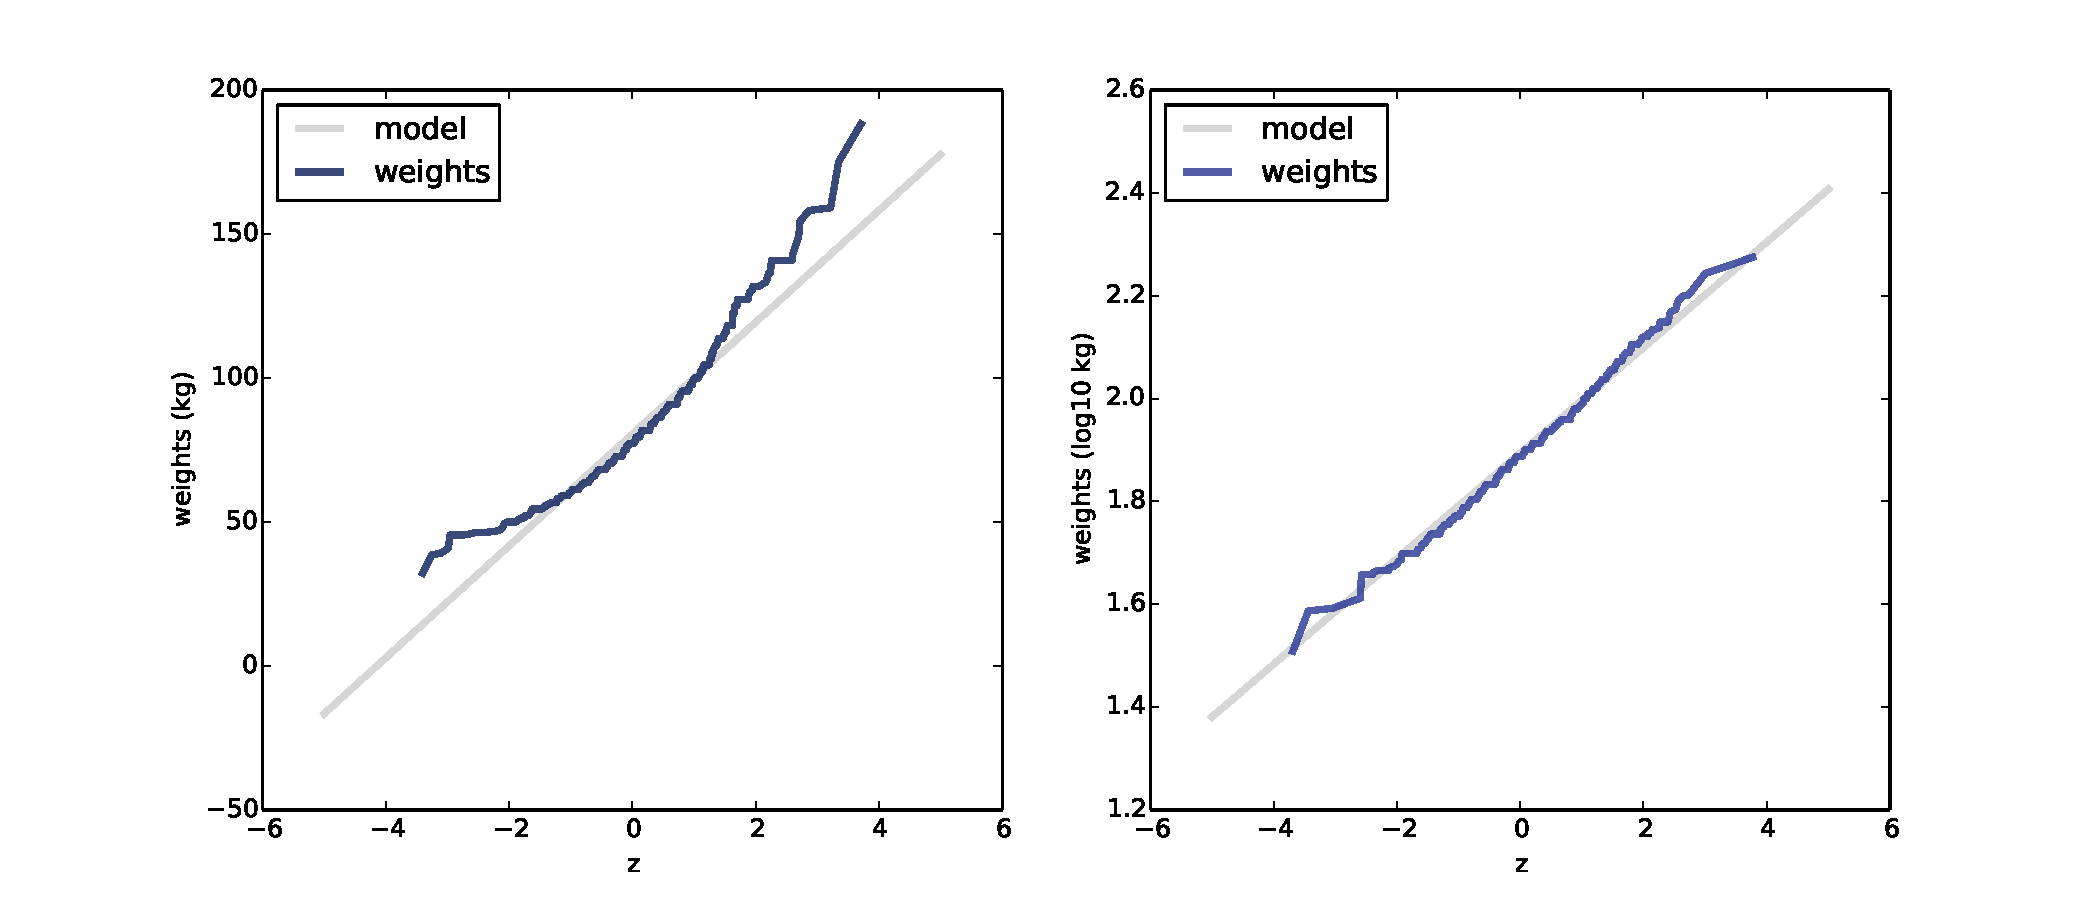
\includegraphics[height=2.5in]{figs/brfss_weight_normal.pdf}}
\caption{Normal probability plots for adult weight on a linear scale
  (left) and log scale (right).}
\label{brfss_weight_normal}
\end{figure}

Figure~\ref{brfss_weight} (left) shows the distribution of adult
weights on a linear scale with a normal model.
Figure~\ref{brfss_weight} (right) shows the same distribution on a log
scale with a lognormal model.  The lognormal model is a better fit,
but this representation of the data does not make the difference
particularly dramatic.  \index{respondent} \index{model}

Figure~\ref{brfss_weight_normal} shows normal probability plots for
adult weights, $w$, and for their logarithms, $\log_{10} w$.  Now it
is apparent that the data deviate substantially from the normal model.
On the other hand, the lognormal model is a good match for the data.
\index{normal distribution} \index{distribution!normal}
\index{Gaussian distribution} \index{distribution!Gaussian}
\index{lognormal distribution} \index{distribution!lognormal}
\index{standard deviation} \index{adult weight} \index{weight!adult}
\index{model} \index{normal probability plot}


\section{The Pareto distribution}
\index{Pareto distribution}
\index{distribution!Pareto}
\index{Pareto, Vilfredo}

The {\bf Pareto distribution} is named after the economist Vilfredo Pareto,
who used it to describe the distribution of wealth (see
\url{http://wikipedia.org/wiki/Pareto_distribution}).  Since then, it
has been used to describe phenomena in the natural and social sciences
including sizes of cities and towns, sand particles and meteorites,
forest fires and earthquakes.  \index{CDF}

The CDF of the Pareto distribution is:
%
\[ CDF(x) = 1 - \left( \frac{x}{x_m} \right) ^{-\alpha} \]
%
The parameters $x_{m}$ and $\alpha$ determine the location and shape
of the distribution. $x_{m}$ is the minimum possible value.
Figure~\ref{analytic_pareto_cdf} shows CDFs of Pareto
distributions with $x_{m} = 0.5$ and different values
of $\alpha$.
\index{parameter}

\begin{figure}
% analytic.py
\centerline{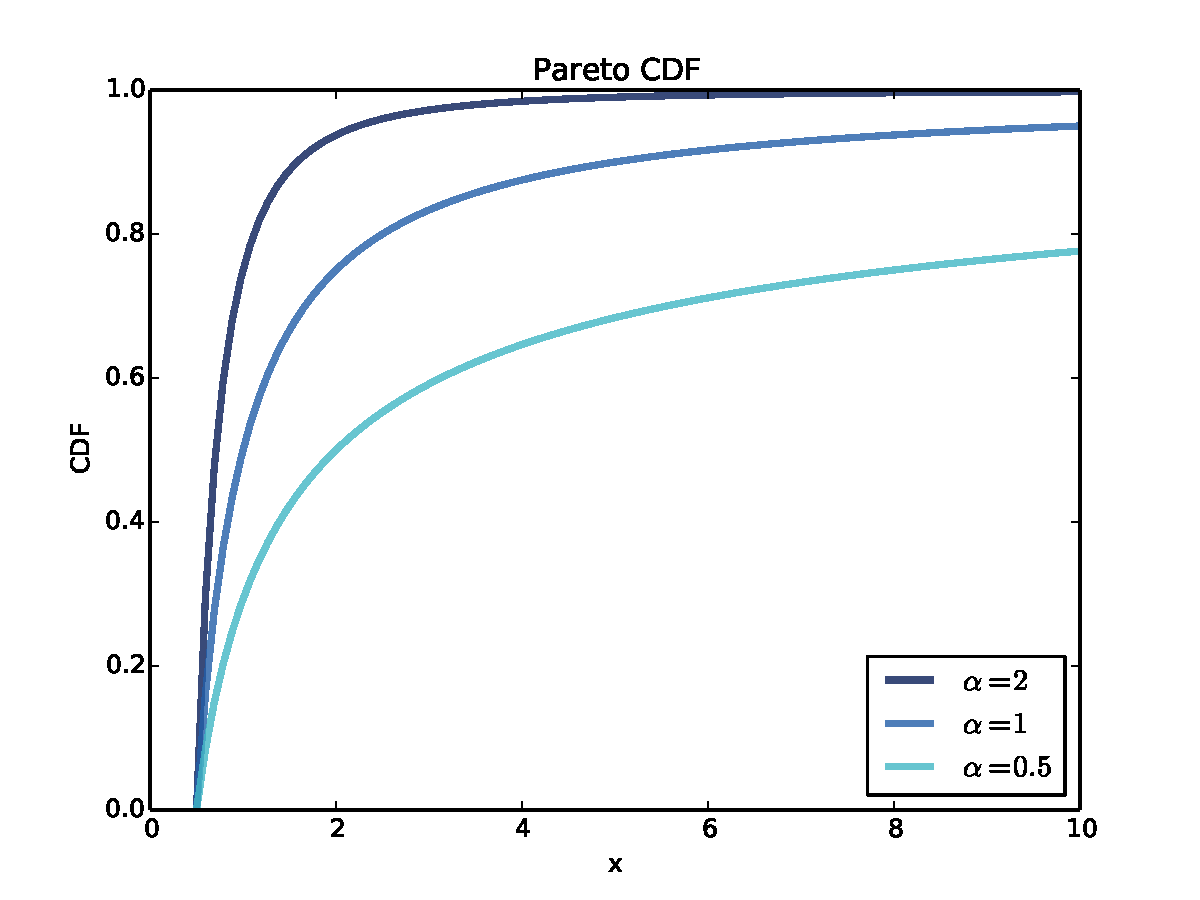
\includegraphics[height=2.5in]{figs/analytic_pareto_cdf.pdf}}
\caption{CDFs of Pareto distributions with different parameters.}
\label{analytic_pareto_cdf}
\end{figure}

There is a simple visual test that indicates whether an empirical
distribution fits a Pareto distribution: on a log-log scale, the CCDF
looks like a straight line.  Let's see why that works.

If you plot the CCDF of a sample from a Pareto distribution on a
linear scale, you expect to see a function like:
%
\[ y \approx \left( \frac{x}{x_m} \right) ^{-\alpha} \]
%
Taking the log of both sides yields:
%
\[ \log y \approx -\alpha (\log x - \log x_{m})\]
%
So if you plot $\log y$ versus $\log x$, it should look like a straight
line with slope $-\alpha$ and intercept
$\alpha \log x_{m}$.

As an example, let's look at the sizes of cities and towns.
The U.S.~Census Bureau publishes the
population of every incorporated city and town in the United States.
\index{Pareto distribution} \index{distribution!Pareto}
\index{U.S.~Census Bureau} \index{population} \index{city size}

\begin{figure}
% populations.py
\centerline{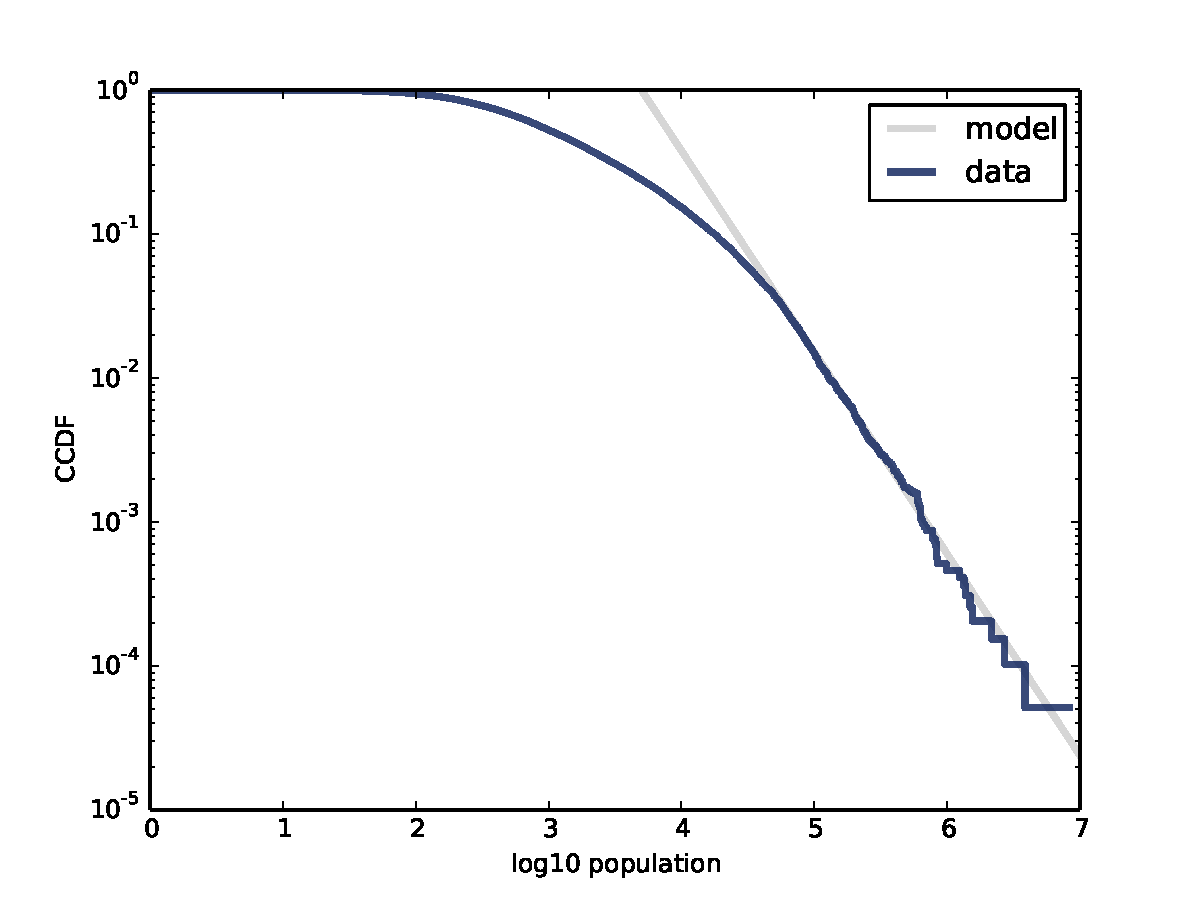
\includegraphics[height=2.5in]{figs/populations_pareto.pdf}}
\caption{CCDFs of city and town populations, on a log-log scale.}
\label{populations_pareto}
\end{figure}

I downloaded their data from
\url{http://www.census.gov/popest/data/cities/totals/2012/SUB-EST2012-3.html};
it is in the repository for this book in a file named
\verb"PEP_2012_PEPANNRES_with_ann.csv".  The repository also
contains {\tt populations.py}, which reads the file and plots
the distribution of populations.

Figure~\ref{populations_pareto} shows the CCDF of populations on a
log-log scale.  The largest 1\% of cities and towns, below $10^{-2}$,
fall along a straight line.  So we could
conclude, as some researchers have, that the tail of this distribution
fits a Pareto model.
\index{model}

On the other hand, a lognormal distribution also models the data well.
Figure~\ref{populations_normal} shows the CDF of populations and a
lognormal model (left), and a normal probability plot (right).  Both
plots show good agreement between the data and the model.
\index{normal probability plot}

Neither model is perfect.
The Pareto model only applies to the largest 1\% of cities, but it
is a better fit for that part of the distribution.  The lognormal
model is a better fit for the other 99\%.
Which model is appropriate depends on which part of the distribution
is relevant.

\begin{figure}
% populations.py
\centerline{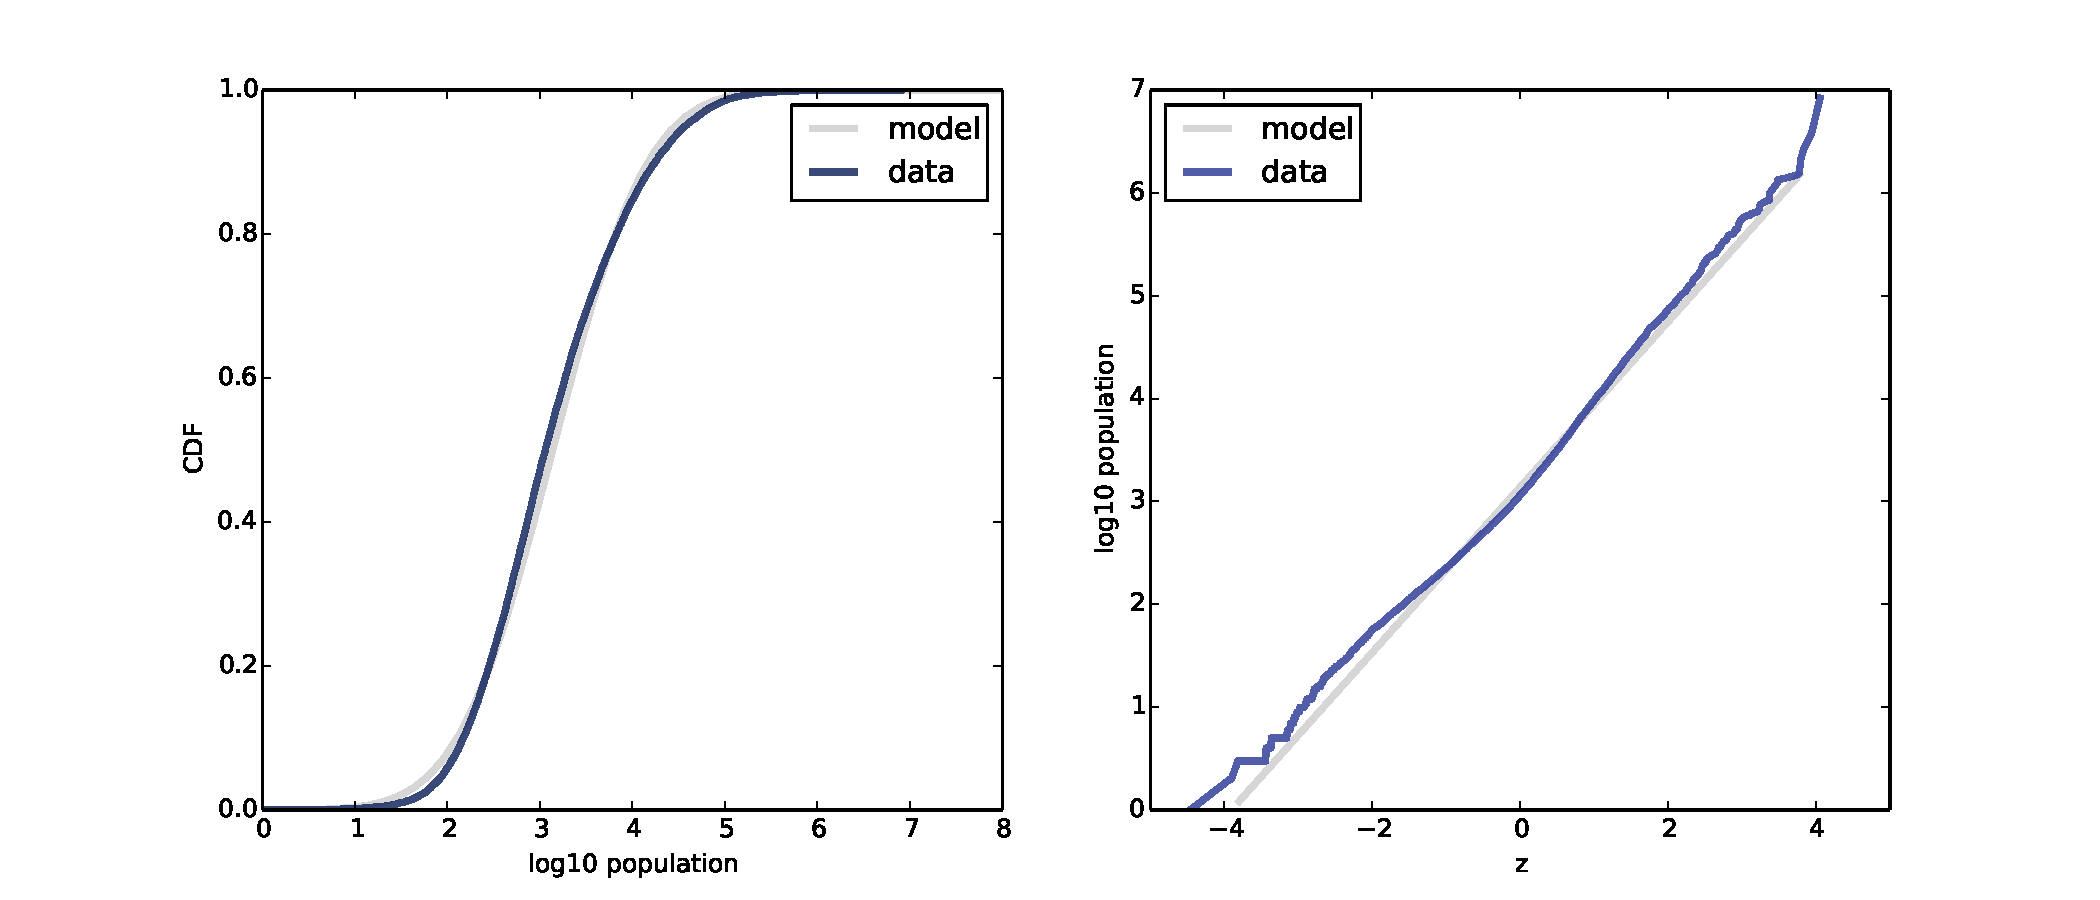
\includegraphics[height=2.5in]{figs/populations_normal.pdf}}
\caption{CDF of city and town populations on a log-x scale (left), and
normal probability plot of log-transformed populations (right).}
\label{populations_normal}
\end{figure}


\section{Generating random numbers}
\index{exponential distribution}
\index{distribution!exponential}
\index{random number}
\index{CDF}
\index{inverse CDF algorithm}
\index{uniform distribution}
\index{distribution!uniform}

Analytic CDFs can be used to generate random numbers with a given
distribution function, $p = \CDF(x)$.  If there is an efficient way to
compute the inverse CDF, we can generate random values
with the appropriate distribution by choosing $p$ from a uniform
distribution between 0 and 1, then choosing
$x = ICDF(p)$.
\index{inverse CDF}
\index{CDF, inverse}

For example, the CDF of the exponential distribution is
%
\[ p = 1 - e^{-\lambda x} \]
%
Solving for $x$ yields:
%
\[ x = -\log (1 - p) / \lambda \]
%
So in Python we can write
%
\begin{verbatim}
def expovariate(lam):
    p = random.random()
    x = -math.log(1-p) / lam
    return x
\end{verbatim}

{\tt expovariate} takes {\tt lam} and returns a random value chosen
from the exponential distribution with parameter {\tt lam}.

Two notes about this implementation:
I called the parameter \verb"lam" because \verb"lambda" is a Python
keyword.  Also, since $\log 0$ is undefined, we have to
be a little careful.  The implementation of {\tt random.random}
can return 0 but not 1, so $1 - p$ can be 1 but not 0, so
{\tt log(1-p)} is always defined.  \index{random module}


\section{Why model?}
\index{model}

At the beginning of this chapter, I said that many real world phenomena
can be modeled with analytic distributions.  ``So,'' you might ask,
``what?''  \index{abstraction}

Like all models, analytic distributions are abstractions, which
means they leave out details that are considered irrelevant.
For example, an observed distribution might have measurement errors
or quirks that are specific to the sample; analytic models smooth
out these idiosyncrasies.
\index{smoothing}

Analytic models are also a form of data compression.  When a model
fits a dataset well, a small set of parameters can summarize a
large amount of data.
\index{parameter}
\index{compression}

It is sometimes surprising when data from a natural phenomenon fit an
analytic distribution, but these observations can provide insight
into physical systems.  Sometimes we can explain why an observed
distribution has a particular form.  For example, Pareto distributions
are often the result of generative processes with positive feedback
(so-called preferential attachment processes: see
\url{http://wikipedia.org/wiki/Preferential_attachment}.).
\index{preferential attachment}
\index{generative process}
\index{Pareto distribution}
\index{distribution!Pareto}
\index{analysis}

Also, analytic distributions lend themselves to mathematical
analysis, as we will see in Chapter~\ref{analysis}.

But it is important to remember that all models are imperfect.
Data from the real world never fit an analytic distribution perfectly.
People sometimes talk as if data are generated by models; for example,
they might say that the distribution of human heights is normal,
or the distribution of income is lognormal.  Taken literally, these
claims cannot be true; there are always differences between the
real world and mathematical models.

Models are useful if they capture the relevant aspects of the
real world and leave out unneeded details.  But what is ``relevant''
or ``unneeded'' depends on what you are planning to use the model
for.


\section{Exercises}

For the following exercises, you can start with \verb"chap05ex.ipynb".
My solution is in \verb"chap05soln.ipynb".

\begin{exercise}
In the BRFSS (see Section~\ref{lognormal}), the distribution of
heights is roughly normal with parameters $\mu = 178$ cm and
$\sigma = 7.7$ cm for men, and $\mu = 163$ cm and $\sigma = 7.3$ cm for
women.
\index{normal distribution}
\index{distribution!normal}
\index{Gaussian distribution}
\index{distribution!Gaussian}
\index{height}
\index{Blue Man Group}
\index{Group, Blue Man}

In order to join Blue Man Group, you have to be male between 5'10''
and 6'1'' (see \url{http://bluemancasting.com}).  What percentage of
the U.S. male population is in this range?  Hint: use {\tt
  scipy.stats.norm.cdf}.
\index{SciPy}

\end{exercise}


\begin{exercise}
To get a feel for the Pareto distribution, let's see how different
the world
would be if the distribution of human height were Pareto.
With the parameters $x_{m} = 1$ m and $\alpha = 1.7$, we
get a distribution with a reasonable minimum, 1 m,
and median, 1.5 m.
\index{height}
\index{Pareto distribution}
\index{distribution!Pareto}

Plot this distribution.  What is the mean human height in Pareto
world?  What fraction of the population is shorter than the mean?  If
there are 7 billion people in Pareto world, how many do we expect to
be taller than 1 km?  How tall do we expect the tallest person to be?
\index{Pareto World}

\end{exercise}


\begin{exercise}
\label{weibull}

The Weibull distribution is a generalization of the exponential
distribution that comes up in failure analysis
(see \url{http://wikipedia.org/wiki/Weibull_distribution}).  Its CDF is
%
\[ CDF(x) = 1 - e^{-(x / \lambda)^k} \]
%
Can you find a transformation that makes a Weibull distribution look
like a straight line?  What do the slope and intercept of the
line indicate?
\index{Weibull distribution}
\index{distribution!Weibull}
\index{exponential distribution}
\index{distribution!exponential}
\index{random module}

Use {\tt random.weibullvariate} to generate a sample from a
Weibull distribution and use it to test your transformation.

\end{exercise}


\begin{exercise}
For small values of $n$, we don't expect an empirical distribution
to fit an analytic distribution exactly.  One way to evaluate
the quality of fit is to generate a sample from an analytic
distribution and see how well it matches the data.
\index{empirical distribution}
\index{distribution!empirical}
\index{random module}

For example, in Section~\ref{exponential} we plotted the distribution
of time between births and saw that it is approximately exponential.
But the distribution is based on only 44 data points.  To see whether
the data might have come from an exponential distribution, generate 44
values from an exponential distribution with the same mean as the
data, about 33 minutes between births.

Plot the distribution of the random values and compare it to the
actual distribution.  You can use {\tt random.expovariate} 
to generate the values.

\end{exercise}

\begin{exercise}
In the repository for this book, you'll find a set of data files
called {\tt mystery0.dat}, {\tt mystery1.dat}, and so on.  Each
contains a sequence of random numbers generated from an analytic
distribution.
\index{random number}

You will also find \verb"test_models.py", a script that reads
data from a file and plots the CDF under a variety of transforms.
You can run it like this:

\begin{verbatim}
$ python test_models.py mystery0.dat
\end{verbatim}

Based on these plots, you should be able to infer what kind of
distribution generated each file.  If you are stumped, you can
look in {\tt mystery.py}, which contains the code that generated
the files.

\end{exercise}


\begin{exercise}
\label{income}

The distributions of wealth and income are sometimes modeled using
lognormal and Pareto distributions.  To see which is better, let's
look at some data.
\index{Pareto distribution}
\index{distribution!Pareto}
\index{lognormal distribution}
\index{distribution!lognormal}

The Current Population Survey (CPS) is a joint effort of the Bureau
of Labor Statistics and the Census Bureau to study income and related
variables.  Data collected in 2013 is available from
\url{http://www.census.gov/hhes/www/cpstables/032013/hhinc/toc.htm}.
I downloaded {\tt hinc06.xls}, which is an Excel spreadsheet with
information about household income, and converted it to {\tt hinc06.csv},
a CSV file you will find in the repository for this book.  You
will also find {\tt hinc.py}, which reads this file.

Extract the distribution of incomes from this dataset.  Are any of the
analytic distributions in this chapter a good model of the data?  A
solution to this exercise is in \url{hinc_soln.py}.
\index{model}

\end{exercise}




\section{Glossary}

\begin{itemize}

\item empirical distribution: The distribution of values in a sample.
  \index{empirical distribution} \index{distribution!empirical}

\item analytic distribution: A distribution whose CDF is an analytic
function.
\index{analytic distribution}
\index{distribution!analytic}

\item model: A useful simplification.  Analytic distributions are
often good models of more complex empirical distributions.
\index{model}

\item interarrival time: The elapsed time between two events.
\index{interarrival time}

\item complementary CDF: A function that maps from a value, $x$,
to the fraction of values that exceed $x$, which is $1 - \CDF(x)$.
\index{complementary CDF} \index{CDF!complementary} \index{CCDF}

\item standard normal distribution: The normal distribution with
mean 0 and standard deviation 1.
\index{standard normal distribution}

\item normal probability plot: A plot of the values in a sample versus
random values from a standard normal distribution.
\index{normal probability plot}
\index{plot!normal probability}

\end{itemize}


\chapter{Probability density functions}
\label{density}
\index{PDF}
\index{probability density function}
\index{exponential distribution}
\index{distribution!exponential}
\index{normal distribution}
\index{distribution!normal}
\index{Gaussian distribution}
\index{distribution!Gaussian}
\index{CDF}
\index{derivative}

The code for this chapter is in {\tt density.py}.  For information
about downloading and working with this code, see Section~\ref{code}.


\section{PDFs}

The derivative of a CDF is called a {\bf probability density function},
or PDF.  For example, the PDF of an exponential distribution is
%
\[ \PDF_{expo}(x) = \lambda e^{-\lambda x}   \]
%
The PDF of a normal distribution is
%
\[ \PDF_{normal}(x) = \frac{1}{\sigma \sqrt{2 \pi}} 
                 \exp \left[ -\frac{1}{2} 
                 \left( \frac{x - \mu}{\sigma} \right)^2 \right]  \]
%
Evaluating a PDF for a particular value of $x$ is usually not useful.
The result is not a probability; it is a probability {\em density}.
\index{density}
\index{mass}

In physics, density is mass per unit of
volume; in order to get a mass, you have to multiply by volume or,
if the density is not constant, you have to integrate over volume.

Similarly, {\bf probability density} measures probability per unit of $x$.
In order to get a probability mass, you have to integrate over $x$.

{\tt thinkstats2} provides a class called Pdf that represents
a probability density function.  Every Pdf object provides the
following methods:

\begin{itemize}

\item {\tt Density}, which takes a value, {\tt x}, and returns the
  density of the distribution at {\tt x}.

\item {\tt Render}, which evaluates the density at a discrete set of
  values and returns a pair of sequences: the sorted values, {\tt xs},
  and their probability densities, {\tt ds}.

\item {\tt MakePmf}, which evaluates {\tt Density}
  at a discrete set of values and returns a normalized Pmf that
  approximates the Pdf.
\index{Pmf}

\item {\tt GetLinspace}, which returns the default set of points used 
  by {\tt Render} and {\tt MakePmf}.

\end{itemize}  

Pdf is an abstract parent class, which means you should not
instantiate it; that is, you cannot create a Pdf object.  Instead, you
should define a child class that inherits from Pdf and provides
definitions of {\tt Density} and {\tt GetLinspace}.  Pdf provides
{\tt Render} and {\tt MakePmf}.

For example, {\tt thinkstats2} provides a class named {\tt
  NormalPdf} that evaluates the normal density function.

\begin{verbatim}
class NormalPdf(Pdf):

    def __init__(self, mu=0, sigma=1, label=''):
        self.mu = mu
        self.sigma = sigma
        self.label = label

    def Density(self, xs):
        return scipy.stats.norm.pdf(xs, self.mu, self.sigma)

    def GetLinspace(self):
        low, high = self.mu-3*self.sigma, self.mu+3*self.sigma
        return np.linspace(low, high, 101)
\end{verbatim}

The NormalPdf object contains the parameters {\tt mu} and
{\tt sigma}.  {\tt Density} uses
{\tt scipy.stats.norm}, which is an object that represents a normal
distribution and provides {\tt cdf} and {\tt pdf}, among other
methods (see Section~\ref{normal}).
\index{SciPy}

The following example creates a NormalPdf with the mean and variance
of adult female heights, in cm, from the BRFSS (see
Section~\ref{brfss}).  Then it computes the density of the
distribution at a location one standard deviation from the mean.
\index{standard deviation}

\begin{verbatim}
>>> mean, var = 163, 52.8
>>> std = math.sqrt(var)
>>> pdf = thinkstats2.NormalPdf(mean, std)
>>> pdf.Density(mean + std)
0.0333001
\end{verbatim}

The result is about 0.03, in units of probability mass per cm.
Again, a probability density doesn't mean much by itself.  But if
we plot the Pdf, we can see the shape of the distribution:

\begin{verbatim}
>>> thinkplot.Pdf(pdf, label='normal')
>>> thinkplot.Show()
\end{verbatim}

{\tt thinkplot.Pdf} plots the Pdf as a smooth function,
as contrasted with {\tt thinkplot.Pmf}, which renders a Pmf as a
step function.  Figure~\ref{pdf_example} shows the result, as well
as a PDF estimated from a sample, which we'll compute in the next
section.
\index{thinkplot}

You can use {\tt MakePmf} to approximate the Pdf:

\begin{verbatim}
>>> pmf = pdf.MakePmf()
\end{verbatim}

By default, the resulting Pmf contains 101 points equally spaced from
{\tt mu - 3*sigma} to {\tt mu + 3*sigma}.  Optionally, {\tt MakePmf}
and {\tt Render} can take keyword arguments {\tt low}, {\tt high},
and {\tt n}.

\begin{figure}
% pdf_example.py
\centerline{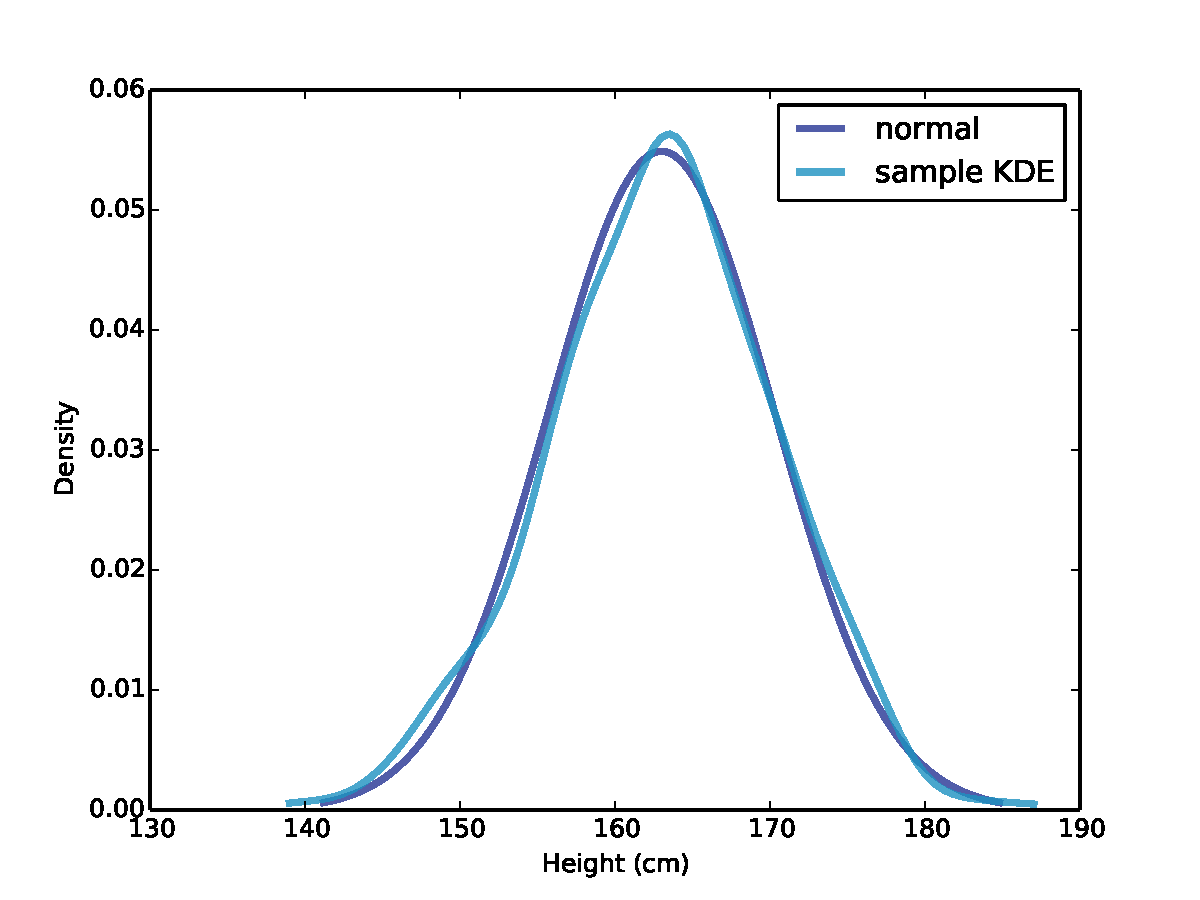
\includegraphics[height=2.2in]{figs/pdf_example.pdf}}
\caption{A normal PDF that models adult female height in the U.S.,
and the kernel density estimate of a sample with $n=500$.}
\label{pdf_example}
\end{figure}


\section{Kernel density estimation} 

{\bf Kernel density estimation} (KDE) is an algorithm that takes
a sample and finds an appropriately smooth PDF that fits 
the data.  You can read details at
\url{http://en.wikipedia.org/wiki/Kernel_density_estimation}.
\index{KDE}
\index{kernel density estimation}

{\tt scipy} provides an implementation of KDE and {\tt thinkstats2}
provides a class called {\tt EstimatedPdf} that uses it:
\index{SciPy}
\index{NumPy}

\begin{verbatim}
class EstimatedPdf(Pdf):

    def __init__(self, sample):
        self.kde = scipy.stats.gaussian_kde(sample)

    def Density(self, xs):
        return self.kde.evaluate(xs)
\end{verbatim}

\verb"__init__" takes a sample
and computes a kernel density estimate.  The result is a
\verb"gaussian_kde" object that provides an {\tt evaluate}
method.

{\tt Density} takes a value or sequence, calls
\verb"gaussian_kde.evaluate", and returns the resulting density.  The
word ``Gaussian'' appears in the name because it uses a filter based
on a Gaussian distribution to smooth the KDE.  \index{density}

Here's an example that generates a sample from a normal
distribution and then makes an EstimatedPdf to fit it:
\index{NumPy}
\index{EstimatedPdf}

\begin{verbatim}
>>> sample = [random.gauss(mean, std) for i in range(500)]
>>> sample_pdf = thinkstats2.EstimatedPdf(sample)
>>> thinkplot.Pdf(sample_pdf, label='sample KDE')
\end{verbatim}

\verb"sample" is a list of 500 random heights.
\verb"sample_pdf" is a Pdf object that contains the estimated
KDE of the sample.
\index{thinkplot}
\index{Pmf}

Figure~\ref{pdf_example} shows the normal density function and a KDE
based on a sample of 500 random heights.  The estimate is a good
match for the original distribution.

Estimating a density function with KDE is useful for several purposes:

\begin{itemize}

\item {\it Visualization:} During the exploration phase of a project, CDFs
  are usually the best visualization of a distribution.  After you
  look at a CDF, you can decide whether an estimated PDF is an
  appropriate model of the distribution.  If so, it can be a better
  choice for presenting the distribution to an audience that is
  unfamiliar with CDFs.
\index{visualization}
\index{model}

\item {\it Interpolation:} An estimated PDF is a way to get from a sample
  to a model of the population.  If you have reason to believe that
  the population distribution is smooth, you can use KDE to interpolate
  the density for values that don't appear in the sample.
\index{interpolation}

\item {\it Simulation:} Simulations are often based on the distribution
  of a sample.  If the sample size is small, it
  might be appropriate to smooth the sample distribution using KDE,
  which allows the simulation to explore more possible outcomes,
  rather than replicating the observed data.
\index{simulation}

\end{itemize}


\section{The distribution framework}
\index{distribution framework}

\begin{figure}
\centerline{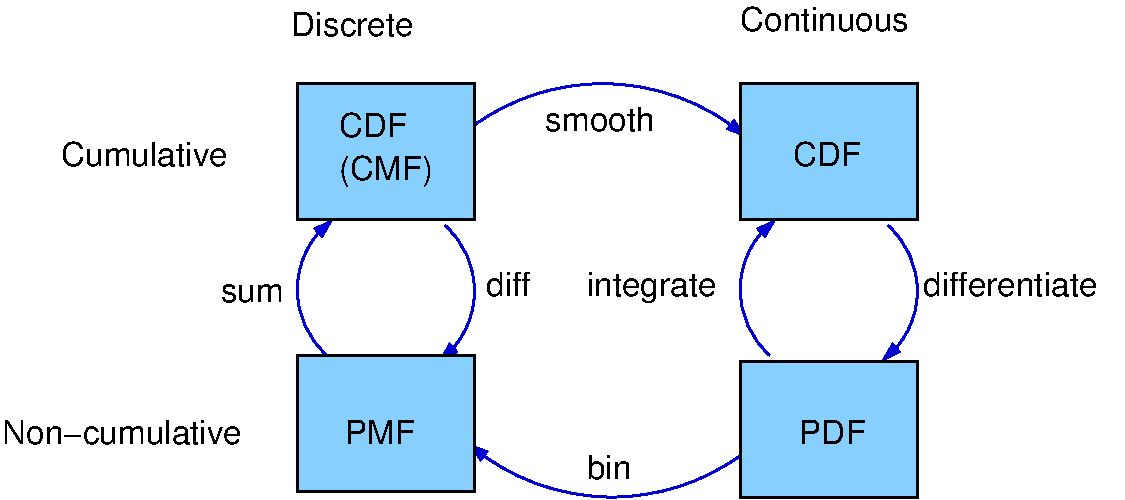
\includegraphics[height=2.2in]{figs/distribution_functions.pdf}}
\caption{A framework that relates representations of distribution
functions.}
\label{dist_framework}
\end{figure}

At this point we have seen PMFs, CDFs and PDFs; let's take a minute
to review.  Figure~\ref{dist_framework} shows how these functions relate
to each other.
\index{Pmf}
\index{Cdf}
\index{Pdf}

We started with PMFs, which represent the probabilities for a discrete
set of values.  To get from a PMF to a CDF, you add up the probability
masses to get cumulative probabilities.  
To get from a CDF back to a PMF, you compute differences in cumulative
probabilities.  We'll see the implementation of these operations
in the next few sections.
\index{cumulative probability}

A PDF is the derivative of a continuous CDF; or, equivalently,
a CDF is the integral of a PDF.  Remember that a PDF maps from
values to probability densities; to get a probability, you have to
integrate.
\index{discrete distribution}
\index{continuous distribution}
\index{smoothing}

To get from a discrete to a continuous distribution, you can perform
various kinds of smoothing.  One form of smoothing is to assume that
the data come from an analytic continuous distribution
(like exponential or normal) and to estimate the parameters of that
distribution.  Another option is kernel density estimation.
\index{exponential distribution}
\index{distribution!exponential}
\index{normal distribution}
\index{distribution!normal}
\index{Gaussian distribution}
\index{distribution!Gaussian}

The opposite of smoothing is {\bf discretizing}, or quantizing.  If you
evaluate a PDF at discrete points, you can generate a PMF that is an
approximation of the PDF.  You can get a better approximation using
numerical integration.  \index{discretize}
\index{quantize}
\index{binning}

To distinguish between continuous and discrete CDFs, it might be
better for a discrete CDF to be a ``cumulative mass function,'' but as
far as I can tell no one uses that term.  \index{CDF}



\section{Hist implementation}

At this point you should know how to use the basic types provided
by {\tt thinkstats2}: Hist, Pmf, Cdf, and Pdf.  The next few sections
provide details about how they are implemented.  This material
might help you use these classes more effectively, but it is not
strictly necessary.
\index{Hist}

Hist and Pmf inherit from a parent class called \verb"_DictWrapper".
The leading underscore indicates that this class is ``internal;'' that
is, it should not be used by code in other modules.  The name
indicates what it is: a dictionary wrapper.  Its primary attribute is
{\tt d}, the dictionary that maps from values to their frequencies.
\index{DictWrapper}
\index{internal class}
\index{wrapper}

The values can be any hashable type.  The frequencies should be integers,
but can be any numeric type.
\index{hashable}

\verb"_DictWrapper" contains methods appropriate for both
Hist and Pmf, including \verb"__init__", {\tt Values},
{\tt Items} and {\tt Render}.  It also provides modifier
methods {\tt Set}, {\tt Incr}, {\tt Mult}, and {\tt Remove}.  These
methods are all implemented with dictionary operations.  For example:
\index{dictionary}

\begin{verbatim}
# class _DictWrapper

    def Incr(self, x, term=1):
        self.d[x] = self.d.get(x, 0) + term

    def Mult(self, x, factor):
        self.d[x] = self.d.get(x, 0) * factor

    def Remove(self, x):
        del self.d[x]
\end{verbatim}

Hist also provides {\tt Freq}, which looks up the frequency
of a given value.
\index{frequency}

Because Hist operators and methods are based on dictionaries,
these methods are constant time operations;
that is, their run time does not increase as the Hist gets bigger.
\index{Hist}


\section{Pmf implementation}

Pmf and Hist are almost the same thing, except that a Pmf
maps values to floating-point probabilities, rather than integer
frequencies.  If the sum of the probabilities is 1, the Pmf is normalized.
\index{Pmf}

Pmf provides {\tt Normalize}, which computes the sum of the
probabilities and divides through by a factor:

\begin{verbatim}
# class Pmf

    def Normalize(self, fraction=1.0):
        total = self.Total()
        if total == 0.0:
            raise ValueError('Total probability is zero.')

        factor = float(fraction) / total
        for x in self.d:
            self.d[x] *= factor

        return total
\end{verbatim}

{\tt fraction} determines the sum of the probabilities after
normalizing; the default value is 1.  If the total probability is 0,
the Pmf cannot be normalized, so {\tt Normalize} raises {\tt
  ValueError}.

Hist and Pmf have the same constructor.  It can take
as an argument a {\tt dict}, Hist, Pmf or Cdf, a pandas
Series, a list of (value, frequency) pairs, or a sequence of values.
\index{Hist}

If you instantiate a Pmf, the result is normalized.  If you
instantiate a Hist, it is not.  To construct an unnormalized Pmf,
you can create an empty Pmf and modify it.  The Pmf modifiers do
not renormalize the Pmf.


\section{Cdf implementation}

A CDF maps from values to cumulative probabilities, so I could have
implemented Cdf as a \verb"_DictWrapper".  But the values in a CDF are
ordered and the values in a \verb"_DictWrapper" are not.  Also, it is
often useful to compute the inverse CDF; that is, the map from
cumulative probability to value.  So the implementaion I chose is two
sorted lists.  That way I can use binary search to do a forward or
inverse lookup in logarithmic time.
\index{Cdf}
\index{binary search}
\index{cumulative probability}
\index{DictWrapper}
\index{inverse CDF}
\index{CDF, inverse}

The Cdf constructor can take as a parameter a sequence of values
or a pandas Series, a dictionary that maps from values to
probabilities, a sequence of (value, probability) pairs, a Hist, Pmf,
or Cdf.  Or if it is given two parameters, it treats them as a sorted
sequence of values and the sequence of corresponding cumulative
probabilities.

Given a sequence, pandas Series, or dictionary, the constructor makes
a Hist.  Then it uses the Hist to initialize the attributes:

\begin{verbatim}
        self.xs, freqs = zip(*sorted(dw.Items()))
        self.ps = np.cumsum(freqs, dtype=np.float)
        self.ps /= self.ps[-1]
\end{verbatim}

{\tt xs} is the sorted list of values; {\tt freqs} is the list
of corresponding frequencies.  {\tt np.cumsum} computes
the cumulative sum of the frequencies.  Dividing through by the
total frequency yields cumulative probabilities.
For {\tt n} values, the time to construct the
Cdf is proportional to $n \log n$.
\index{frequency}

Here is the implementation of {\tt Prob}, which takes a value
and returns its cumulative probability: 

\begin{verbatim}
# class Cdf
    def Prob(self, x):
        if x < self.xs[0]:
            return 0.0
        index = bisect.bisect(self.xs, x)
        p = self.ps[index - 1]
        return p
\end{verbatim}

The {\tt bisect} module provides an implementation of binary search.
And here is the implementation of {\tt Value}, which takes a
cumulative probability and returns the corresponding value:

\begin{verbatim}
# class Cdf
    def Value(self, p):
        if p < 0 or p > 1:
            raise ValueError('p must be in range [0, 1]')

        index = bisect.bisect_left(self.ps, p)
        return self.xs[index]
\end{verbatim}

Given a Cdf, we can compute the Pmf by computing differences between
consecutive cumulative probabilities.  If you call the Cdf constructor
and pass a Pmf, it computes differences by calling {\tt Cdf.Items}:
\index{Pmf}
\index{Cdf}

\begin{verbatim}
# class Cdf
    def Items(self):
        a = self.ps
        b = np.roll(a, 1)
        b[0] = 0
        return zip(self.xs, a-b)
\end{verbatim}

{\tt np.roll} shifts the elements of {\tt a} to the right, and ``rolls''
the last one back to the beginning.  We replace the first element of
{\tt b} with 0 and then compute the difference {\tt a-b}.  The result
is a NumPy array of probabilities.
\index{NumPy}

Cdf provides {\tt Shift} and {\tt Scale}, which modify the
values in the Cdf, but the probabilities should be treated as
immutable.


\section{Moments}
\index{moment}

Any time you take a sample and reduce it to a single number, that
number is a statistic.  The statistics we have seen so far include
mean, variance, median, and interquartile range.

A {\bf raw moment} is a kind of statistic.  If you have a sample of
values, $x_i$, the $k$th raw moment is:
%
\[ m'_k = \frac{1}{n} \sum_i x_i^k \]
%
Or if you prefer Python notation:

\begin{verbatim}
def RawMoment(xs, k):
    return sum(x**k for x in xs) / len(xs)
\end{verbatim}

When $k=1$ the result is the sample mean, $\xbar$.  The other
raw moments don't mean much by themselves, but they are used
in some computations.

The {\bf central moments} are more useful.  The
$k$th central moment is:
%
\[ m_k = \frac{1}{n} \sum_i (x_i - \xbar)^k \]
%
Or in Python:

\begin{verbatim}
def CentralMoment(xs, k):
    mean = RawMoment(xs, 1)
    return sum((x - mean)**k for x in xs) / len(xs)
\end{verbatim}

When $k=2$ the result is the second central moment, which you might
recognize as variance.  The definition of variance gives a hint about
why these statistics are called moments.  If we attach a weight along a
ruler at each location, $x_i$, and then spin the ruler around
the mean, the moment of inertia of the spinning weights is the variance
of the values.  If you are not familiar with moment of inertia, see
\url{http://en.wikipedia.org/wiki/Moment_of_inertia}.  \index{moment
  of inertia}

When you report moment-based statistics, it is important to think
about the units.  For example, if the values $x_i$ are in cm, the
first raw moment is also in cm.  But the second moment is in
cm$^2$, the third moment is in cm$^3$, and so on.

Because of these units, moments are hard to interpret by themselves.
That's why, for the second moment, it is common to report standard
deviation, which is the square root of variance, so it is in the same
units as $x_i$.
\index{standard deviation}


\section{Skewness}
\index{skewness}

{\bf Skewness} is a property that describes the shape of a distribution.
If the distribution is symmetric around its central tendency, it is
unskewed.  If the values extend farther to the right, it is ``right
skewed'' and if the values extend left, it is ``left skewed.''
\index{central tendency}

This use of ``skewed'' does not have the usual connotation of
``biased.''  Skewness only describes the shape of the distribution;
it says nothing about whether the sampling process might have been
biased.
\index{bias}
\index{sample skewness}

Several statistics are commonly used to quantify the skewness of a
distribution.  Given a sequence of values, $x_i$, the {\bf sample
  skewness}, $g_1$, can be computed like this:

\begin{verbatim}
def StandardizedMoment(xs, k):
    var = CentralMoment(xs, 2)
    std = math.sqrt(var)
    return CentralMoment(xs, k) / std**k

def Skewness(xs):
    return StandardizedMoment(xs, 3)
\end{verbatim}

$g_1$ is the third {\bf standardized moment}, which means that it has
been normalized so it has no units.
\index{standardized moment}

Negative skewness indicates that a distribution 
skews left; positive skewness indicates
that a distribution skews right.  The magnitude of $g_1$ indicates
the strength of the skewness, but by itself it is not easy to
interpret.

In practice, computing sample skewness is usually not
a good idea.  If there are any outliers, they
have a disproportionate effect on $g_1$.
\index{outlier}

Another way to evaluate the asymmetry of a distribution is to look
at the relationship between the mean and median.
Extreme values have more effect on the mean than the median, so
in a distribution that skews left, the mean is less than the median.
In a distribution that skews right, the mean is greater.
\index{symmetric}
\index{Pearson median skewness}

{\bf Pearson's median skewness coefficient} is a measure
of skewness based on the difference between the
sample mean and median:
%
\[ g_p = 3 (\xbar - m) / S \]
%
Where $\xbar$ is the sample mean, $m$ is the median, and
$S$ is the standard deviation.  Or in Python:
\index{standard deviation}

\begin{verbatim}
def Median(xs):
    cdf = thinkstats2.Cdf(xs)
    return cdf.Value(0.5)

def PearsonMedianSkewness(xs):
    median = Median(xs)
    mean = RawMoment(xs, 1)
    var = CentralMoment(xs, 2)
    std = math.sqrt(var)
    gp = 3 * (mean - median) / std
    return gp
\end{verbatim}

This statistic is {\bf robust}, which means that it is less vulnerable
to the effect of outliers.
\index{robust}
\index{outlier}

\begin{figure}
\centerline{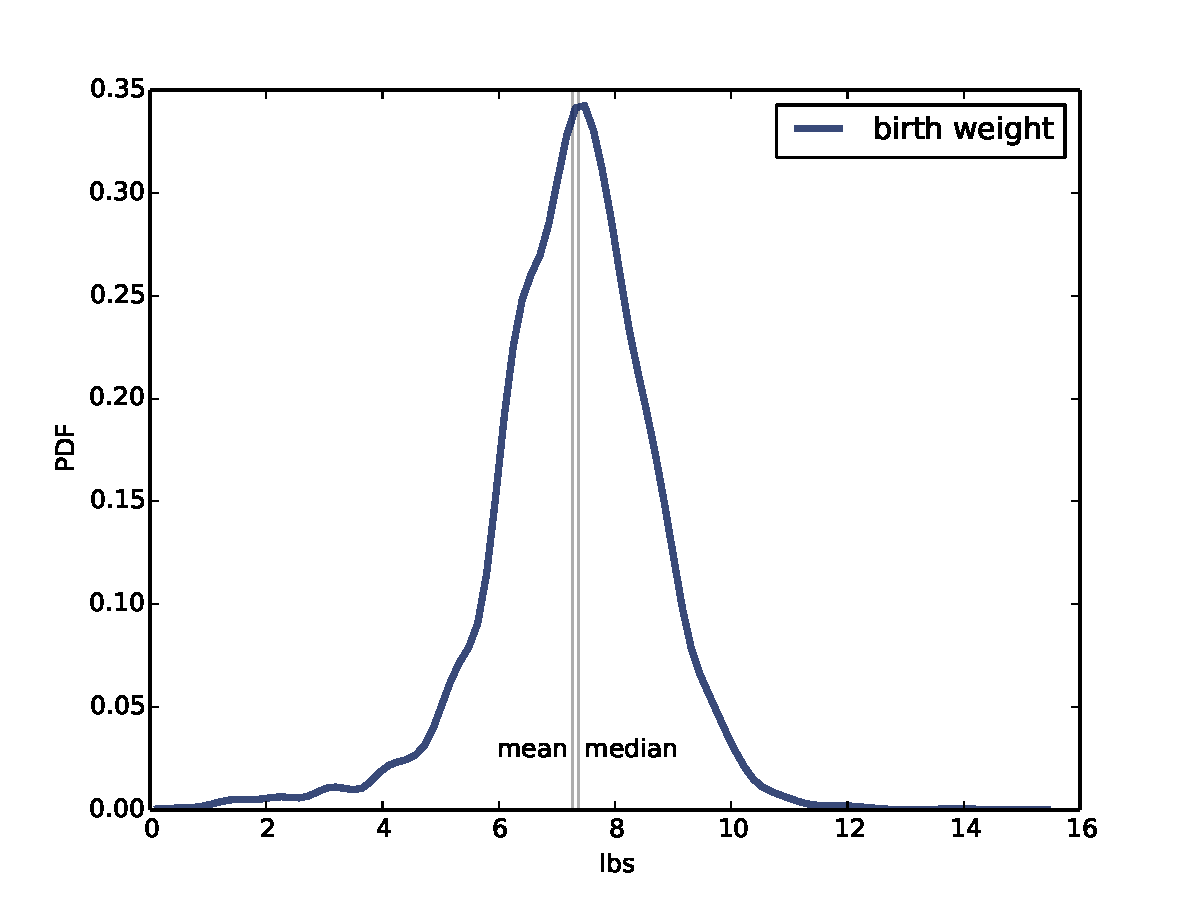
\includegraphics[height=2.2in]{figs/density_totalwgt_kde.pdf}}
\caption{Estimated PDF of birthweight data from the NSFG.}
\label{density_totalwgt_kde}
\end{figure}

As an example, let's look at the skewness of birth weights in the
NSFG pregnancy data.  Here's the code to estimate and plot the PDF:
\index{thinkplot}

\begin{verbatim}
    live, firsts, others = first.MakeFrames()
    data = live.totalwgt_lb.dropna()
    pdf = thinkstats2.EstimatedPdf(data)
    thinkplot.Pdf(pdf, label='birth weight')
\end{verbatim}

Figure~\ref{density_totalwgt_kde} shows the result.  The left tail appears
longer than the right, so we suspect the distribution is skewed left.
The mean, 7.27 lbs, is a bit less than
the median, 7.38 lbs, so that is consistent with left skew.
And both skewness coefficients are negative:
sample skewness is -0.59;
Pearson's median skewness is -0.23.
\index{skewness}
\index{dropna}
\index{NaN}

\begin{figure}
\centerline{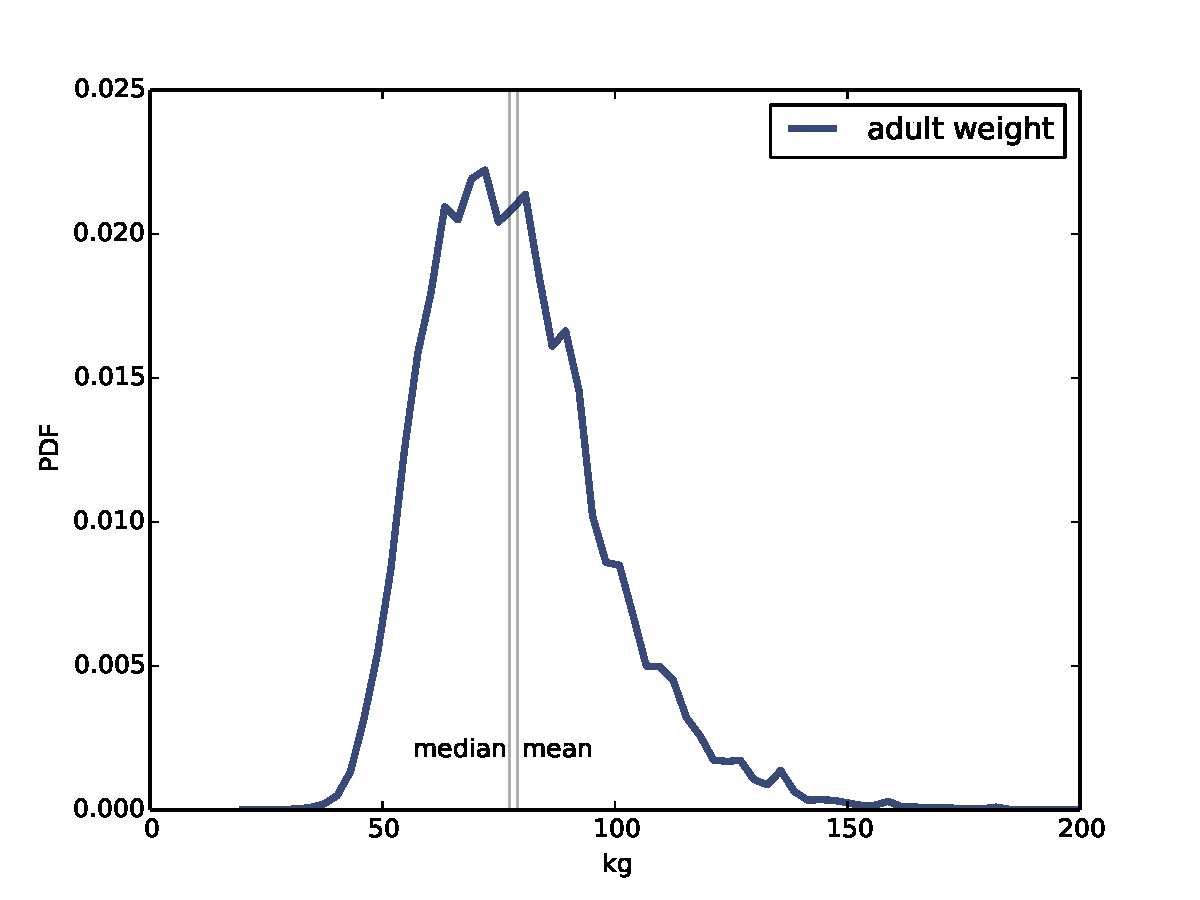
\includegraphics[height=2.2in]{figs/density_wtkg2_kde.pdf}}
\caption{Estimated PDF of adult weight data from the BRFSS.}
\label{density_wtkg2_kde}
\end{figure}

Now let's compare this distribution to the distribution of adult
weight in the BRFSS.  Again, here's the code:
\index{thinkplot}

\begin{verbatim}
    df = brfss.ReadBrfss(nrows=None)
    data = df.wtkg2.dropna()
    pdf = thinkstats2.EstimatedPdf(data)
    thinkplot.Pdf(pdf, label='adult weight')
\end{verbatim}

Figure~\ref{density_wtkg2_kde} shows the result.  The distribution
appears skewed to the right.  Sure enough, the mean, 79.0, is bigger
than the median, 77.3.  The sample skewness is 1.1 and Pearson's
median skewness is 0.26.
\index{dropna}
\index{NaN}

The sign of the skewness coefficient indicates whether the distribution
skews left or right, but other than that, they are hard to interpret.
Sample skewness is less robust; that is, it is more
susceptible to outliers.  As a result it is less reliable
when applied to skewed distributions, exactly when it would be most
relevant.
\index{outlier}
\index{robust}

Pearson's median skewness is based on a computed mean and variance,
so it is also susceptible to outliers, but since it does not depend
on a third moment, it is somewhat more robust.
\index{Pearson median skewness}


\section{Exercises}

A solution to this exercise is in \verb"chap06soln.py".

\begin{exercise}

The distribution of income is famously skewed to the right.  In this
exercise, we'll measure how strong that skew is.
\index{skewness}
\index{income}

The Current Population Survey (CPS) is a joint effort of the Bureau
of Labor Statistics and the Census Bureau to study income and related
variables.  Data collected in 2013 is available from
\url{http://www.census.gov/hhes/www/cpstables/032013/hhinc/toc.htm}.
I downloaded {\tt hinc06.xls}, which is an Excel spreadsheet with
information about household income, and converted it to {\tt hinc06.csv},
a CSV file you will find in the repository for this book.  You
will also find {\tt hinc2.py}, which reads this file and transforms
the data.
\index{Current Population Survey}
\index{Bureau of Labor Statistics}
\index{Census Bureau}

The dataset is in the form of a series of income ranges and the number
of respondents who fell in each range.  The lowest range includes
respondents who reported annual household income ``Under \$5000.''
The highest range includes respondents who made ``\$250,000 or
more.''

To estimate mean and other statistics from these data, we have to
make some assumptions about the lower and upper bounds, and how
the values are distributed in each range.  {\tt hinc2.py} provides
{\tt InterpolateSample}, which shows one way to model
this data.  It takes a DataFrame with a column, {\tt income}, that
contains the upper bound of each range, and {\tt freq}, which contains
the number of respondents in each frame.
\index{DataFrame}
\index{model}

It also takes \verb"log_upper", which is an assumed upper bound
on the highest range, expressed in {\tt log10} dollars.  
The default value, \verb"log_upper=6.0" represents the assumption
that the largest income among the respondents is
$10^6$, or one million dollars.

{\tt InterpolateSample} generates a pseudo-sample; that is, a sample
of household incomes that yields the same number of respondents
in each range as the actual data.  It assumes that incomes in
each range are equally spaced on a log10 scale.

Compute the median, mean, skewness and Pearson's skewness of the
resulting sample.  What fraction of households reports a taxable
income below the mean?  How do the results depend on the assumed
upper bound?
\end{exercise}


\section{Glossary}

\begin{itemize}

\item Probability density function (PDF): The derivative of a continuous CDF,
a function that maps a value to its probability density.
\index{PDF}
\index{probability density function}

\item Probability density: A quantity that can be integrated over a
  range of values to yield a probability.  If the values are in units
  of cm, for example, probability density is in units of probability
  per cm.
\index{probability density}

\item Kernel density estimation (KDE): An algorithm that estimates a PDF
based on a sample.
\index{kernel density estimation}
\index{KDE}

\item discretize: To approximate a continuous function or distribution
with a discrete function.  The opposite of smoothing.
\index{discretize}

\item raw moment: A statistic based on the sum of data raised to a power.
\index{raw moment}

\item central moment: A statistic based on deviation from the mean,
raised to a power.
\index{central moment}

\item standardized moment: A ratio of moments that has no units.
\index{standardized moment}

\item skewness: A measure of how asymmetric a distribution is.
\index{skewness}

\item sample skewness: A moment-based statistic intended to quantify
the skewness of a distribution.
\index{sample skewness}

\item Pearson's median skewness coefficient: A statistic intended to
  quantify the skewness of a distribution based on the median, mean,
  and standard deviation.
  \index{Pearson median skewness}

\item robust: A statistic is robust if it is relatively immune to the
  effect of outliers.
\index{robust}

\end{itemize}



\chapter{Relationships between variables}

So far we have only looked at one variable at a time.  In this
chapter we look at relationships between variables.  Two variables are
related if knowing one gives you information about the other.  For
example, height and weight are related; people who are taller tend to
be heavier.  Of course, it is not a perfect relationship: there
are short heavy people and tall light ones.  But if you are
trying to guess someone's weight, you will be more accurate if you
know their height than if you don't.
\index{adult weight}
\index{adult height}

The code for this chapter is in {\tt scatter.py}.
For information about downloading and
working with this code, see Section~\ref{code}.


\section{Scatter plots}
\index{scatter plot}
\index{plot!scatter}

The simplest way to check for a relationship between two variables
is a {\bf scatter plot}, but making a good scatter plot is not always easy.
As an example, I'll plot weight versus height for the respondents
in the BRFSS (see Section~\ref{lognormal}).
\index{BRFSS}

Here's the code that reads the data file and extracts height and
weight:

\begin{verbatim}
    df = brfss.ReadBrfss(nrows=None)
    sample = thinkstats2.SampleRows(df, 5000)
    heights, weights = sample.htm3, sample.wtkg2
\end{verbatim}

{\tt SampleRows} chooses a random subset of the data:
\index{SampleRows}

\begin{verbatim}
def SampleRows(df, nrows, replace=False):
    indices = np.random.choice(df.index, nrows, replace=replace)
    sample = df.loc[indices]
    return sample
\end{verbatim}

{\tt df} is the DataFrame, {\tt nrows} is the number of rows to choose,
and {\tt replace} is a boolean indicating whether sampling should be
done with replacement; in other words, whether the same row could be
chosen more than once.
\index{DataFrame}
\index{thinkplot}
\index{boolean}
\index{replacement}

{\tt thinkplot} provides {\tt Scatter}, which makes scatter plots:
%
\begin{verbatim}
    thinkplot.Scatter(heights, weights)
    thinkplot.Show(xlabel='Height (cm)',
                   ylabel='Weight (kg)',
                   axis=[140, 210, 20, 200])
\end{verbatim}

The result, in Figure~\ref{scatter1} (left), shows the shape of
the relationship.  As we expected, taller
people tend to be heavier.  

\begin{figure}
% scatter.py
\centerline{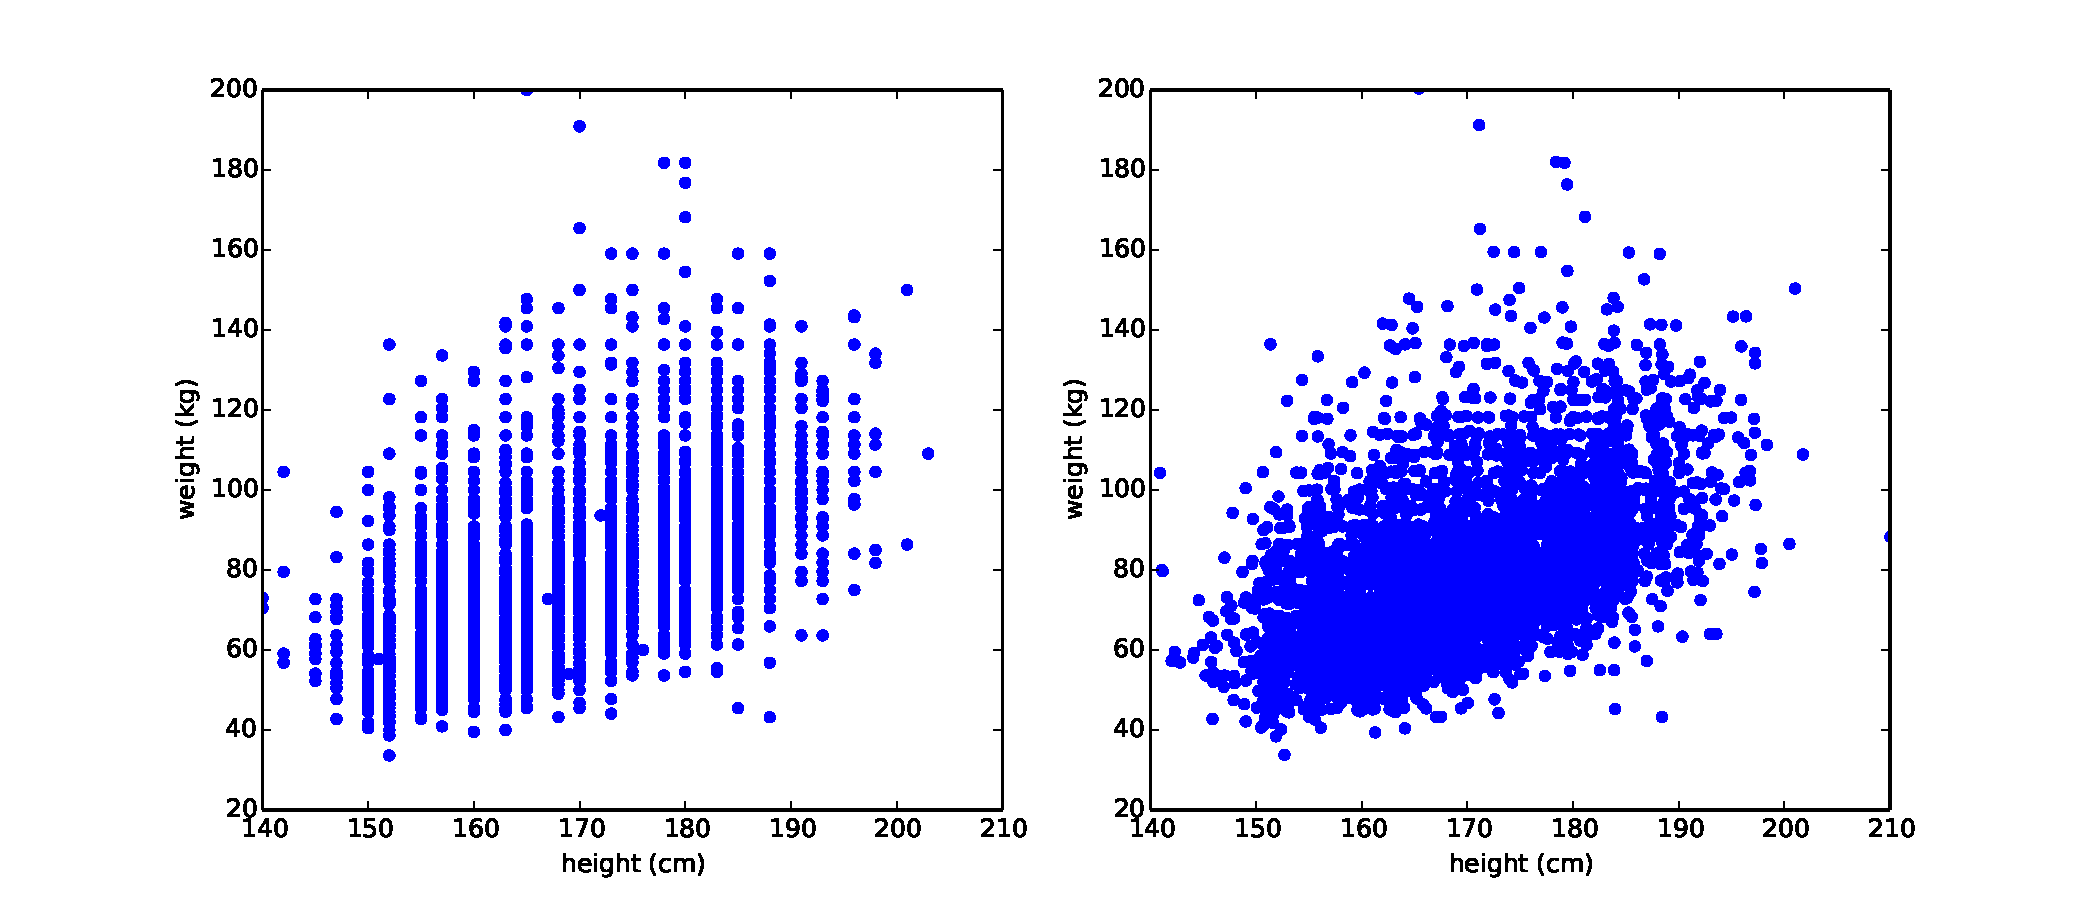
\includegraphics[height=3.0in]{figs/scatter1.pdf}}
\caption{Scatter plots of weight versus height for the respondents
in the BRFSS, unjittered (left), jittered (right).}
\label{scatter1}
\end{figure}

But this is not the best representation of
the data, because the data are packed into columns.  The problem is
that the heights are rounded to the nearest inch, converted to
centimeters, and then rounded again.  Some information is lost in
translation.  \index{height} \index{weight} \index{jitter}

We can't get that information back, but we can minimize the effect on
the scatter plot by {\bf jittering} the data, which means adding random
noise to reverse the effect of rounding off.  Since these measurements
were rounded to the nearest inch, they might be off by up to 0.5 inches or
1.3 cm.  Similarly, the weights might be off by 0.5 kg.
\index{uniform distribution}
\index{distribution!uniform}
\index{noise}

%
\begin{verbatim}
    heights = thinkstats2.Jitter(heights, 1.3)
    weights = thinkstats2.Jitter(weights, 0.5)
\end{verbatim}

Here's the implementation of {\tt Jitter}:

\begin{verbatim}
def Jitter(values, jitter=0.5):
    n = len(values)
    return np.random.uniform(-jitter, +jitter, n) + values
\end{verbatim}

The values can be any sequence; the result is a NumPy array.
\index{NumPy}

Figure~\ref{scatter1} (right) shows the result.  Jittering reduces the
visual effect of rounding and makes the shape of the relationship
clearer.  But in general you should only jitter data for purposes of
visualization and avoid using jittered data for analysis.

Even with jittering, this is not the best way to represent the data.
There are many overlapping points, which hides data
in the dense parts of the figure and gives disproportionate emphasis
to outliers.  This effect is called {\bf saturation}.
\index{outlier}
\index{saturation}

\begin{figure}
% scatter.py
\centerline{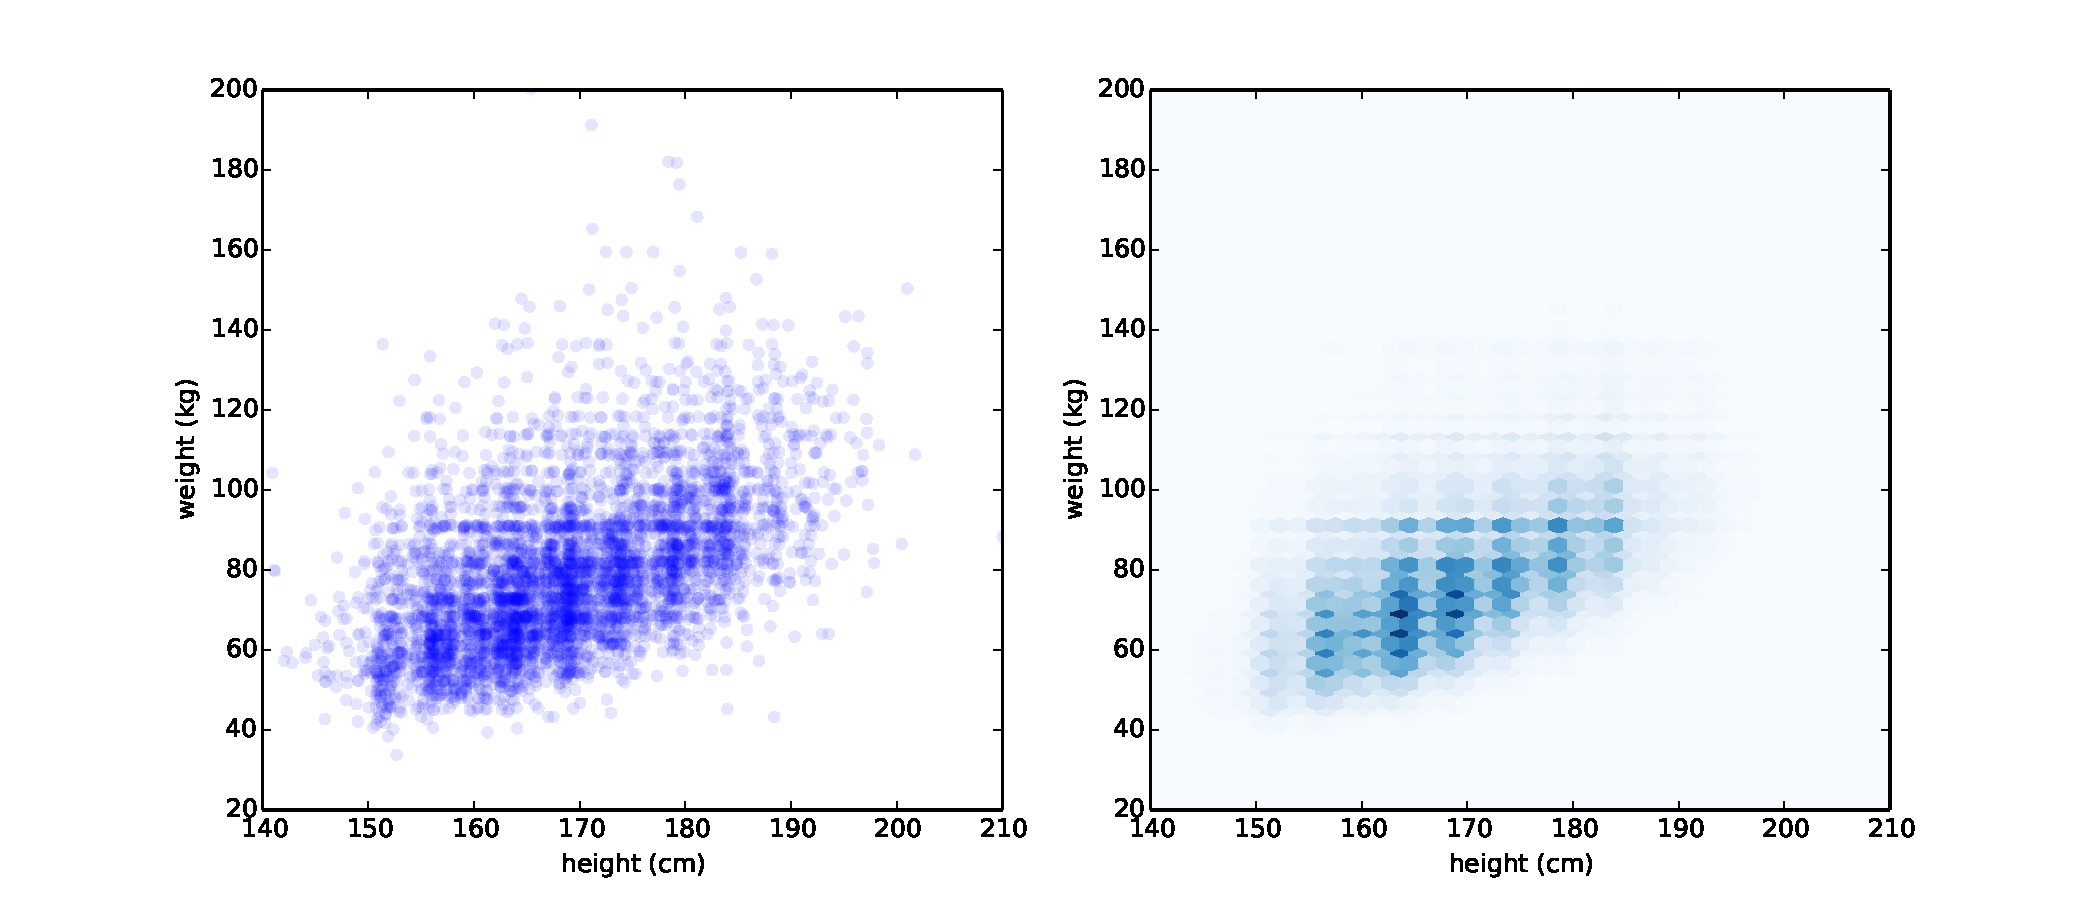
\includegraphics[height=3.0in]{figs/scatter2.pdf}}
\caption{Scatter plot with jittering and transparency (left),
hexbin plot (right).}
\label{scatter2}
\end{figure}

We can solve this problem with the {\tt alpha} parameter, which makes
the points partly transparent:
%
\begin{verbatim}
    thinkplot.Scatter(heights, weights, alpha=0.2)
\end{verbatim}
%
Figure~\ref{scatter2} (left) shows the result.  Overlapping data
points look darker, so darkness is proportional to density.  In this
version of the plot we can see two details that were not apparent before:
vertical clusters at several heights and a horizontal line near 90 kg
or 200 pounds.  Since this data is based on self-reports in pounds,
the most likely explanation is that some respondents reported
rounded values.
\index{thinkplot}
\index{alpha}
\index{transparency}

Using transparency works well for moderate-sized datasets, but this
figure only shows the first 5000 records in the BRFSS, out of a total
of 414 509.
\index{hexbin plot}
\index{plot!hexbin}

To handle larger datasets, another option is a hexbin plot, which
divides the graph into hexagonal bins and colors each bin according to
how many data points fall in it.  {\tt thinkplot} provides 
{\tt HexBin}:
%
\begin{verbatim}
    thinkplot.HexBin(heights, weights)
\end{verbatim}
%
Figure~\ref{scatter2} (right) shows the result.  An advantage of a
hexbin is that it shows the shape of the relationship well, and it is
efficient for large datasets, both in time and in the size of the file
it generates.  A drawback is that it makes the outliers invisible.
\index{thinkplot}
\index{outlier}

The point of this example is that it is
not easy to make a scatter plot that shows relationships clearly
without introducing misleading artifacts.
\index{artifact}


\section{Characterizing relationships}
\label{characterizing}

Scatter plots provide a general impression of the relationship between
variables, but there are other visualizations that provide more
insight into the nature of the relationship.  One option is to bin one
variable and plot percentiles of the other.
\index{binning}

NumPy and pandas provide functions for binning data:
\index{NumPy}
\index{pandas}

\begin{verbatim}
    df = df.dropna(subset=['htm3', 'wtkg2'])
    bins = np.arange(135, 210, 5)
    indices = np.digitize(df.htm3, bins)
    groups = df.groupby(indices)
\end{verbatim}

{\tt dropna} drops rows with {\tt nan} in any of the listed columns.
{\tt arange} makes a NumPy array of bins from 135 to, but not including,
210, in increments of 5.
\index{dropna}
\index{digitize}
\index{NaN}

{\tt digitize} computes the index of the bin that contains each value
in {\tt df.htm3}.  The result is a NumPy array of integer indices.
Values that fall below the lowest bin are mapped to index 0.  Values
above the highest bin are mapped to {\tt len(bins)}.

\begin{figure}
% scatter.py
\centerline{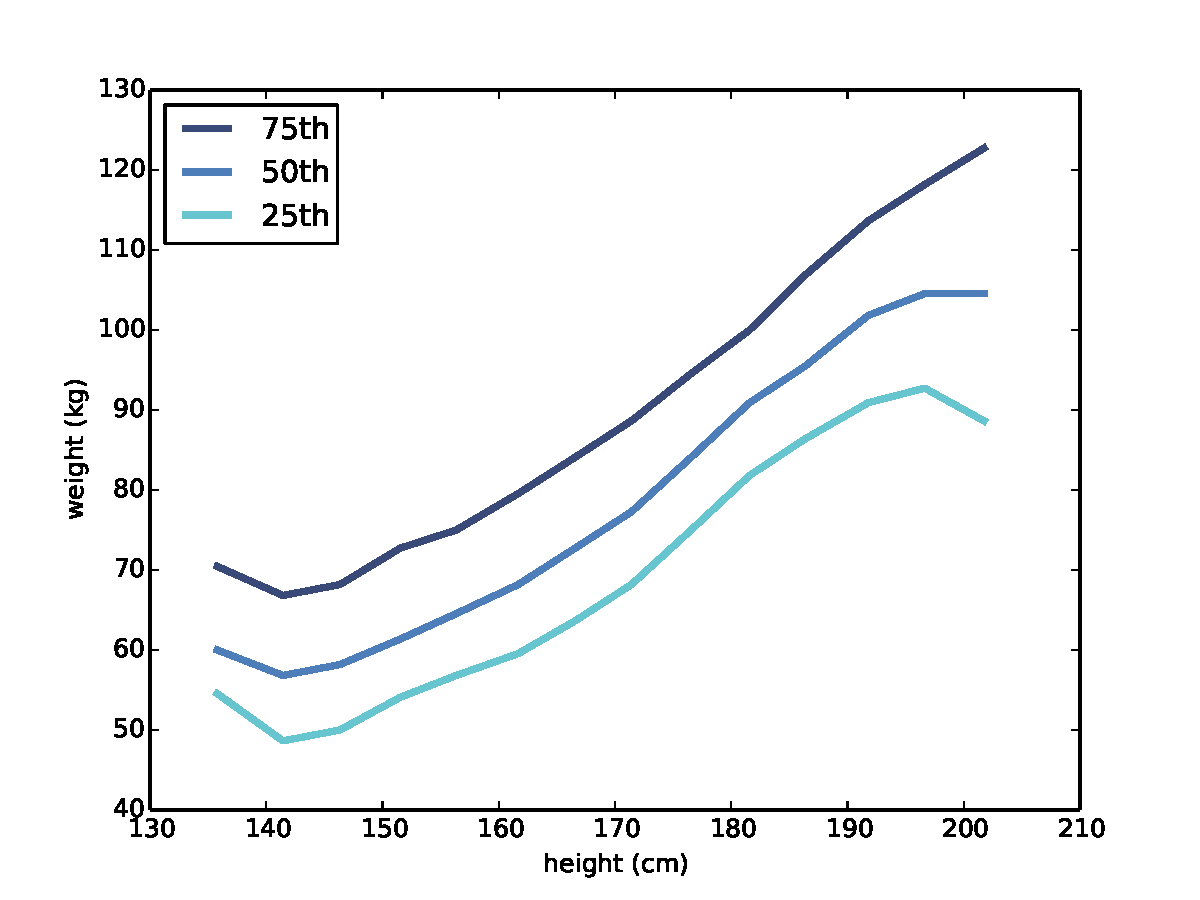
\includegraphics[height=2.5in]{figs/scatter3.pdf}}
\caption{Percentiles of weight for a range of height bins.}
\label{scatter3}
\end{figure}

{\tt groupby} is a DataFrame method that returns a GroupBy object;
used in a {\tt for} loop, {\tt groups} iterates the names of the groups
and the DataFrames that represent them.  So, for example, we can
print the number of rows in each group like this:
\index{DataFrame}
\index{groupby}

\begin{verbatim}
for i, group in groups:
    print(i, len(group))
\end{verbatim}

Now for each group we can compute the mean height and the CDF
of weight:
\index{Cdf}

\begin{verbatim}
    heights = [group.htm3.mean() for i, group in groups]
    cdfs = [thinkstats2.Cdf(group.wtkg2) for i, group in groups]
\end{verbatim}

Finally, we can
plot percentiles of weight versus height:
\index{percentile}

\begin{verbatim}
    for percent in [75, 50, 25]:
        weights = [cdf.Percentile(percent) for cdf in cdfs]
        label = '%dth' % percent
        thinkplot.Plot(heights, weights, label=label)
\end{verbatim}

Figure~\ref{scatter3} shows the result.  Between 140 and 200 cm
the relationship between these variables is roughly linear.  This range
includes more than 99\% of the data, so we don't have to worry
too much about the extremes.
\index{thinkplot}


\section{Correlation}

A {\bf correlation} is a statistic intended to quantify the strength
of the relationship between two variables.
\index{correlation}

A challenge in measuring correlation is that the variables we want to
compare are often not expressed in the same units.  And even if they
are in the same units, they come from different distributions.
\index{units}

There are two common solutions to these problems:

\begin{enumerate}

\item Transform each value to a {\bf standard scores}, which is the
number of standard deviations from the mean.  
This transform leads to
the ``Pearson product-moment correlation coefficient.''
\index{standard score}
\index{standard deviation}
\index{Pearson coefficient of correlation}

\item Transform each value to its {\bf rank}, which is its index in
the sorted list of values.  This transform
leads to the ``Spearman rank correlation coefficient.''
\index{rank}
\index{percentile rank}
\index{Spearman coefficient of correlation}

\end{enumerate}

If $X$ is a series of $n$ values, $x_i$, we can convert to standard
scores by subtracting the mean and dividing by the standard deviation:
$z_i = (x_i - \mu) / \sigma$.
\index{mean}
\index{standard deviation}

The numerator is a deviation: the distance from the mean.  Dividing by
$\sigma$ {\bf standardizes} the deviation, so the values of $Z$ are
dimensionless (no units) and their distribution has mean 0 and
variance 1.
\index{standardize}
\index{deviation}
\index{normal distribution}
\index{distribution!normal}
\index{Gaussian distribution}
\index{distribution!Gaussian}

If $X$ is normally distributed, so is $Z$.  But if $X$ is skewed or has
outliers, so does $Z$; in those cases, it is more robust to use
percentile ranks.  If we compute a new variable, $R$, so that $r_i$ is
the rank of $x_i$, the distribution of $R$ is uniform
from 1 to $n$, regardless of the distribution of $X$.
\index{uniform distribution} \index{distribution!uniform}
\index{robust}
\index{skewness}
\index{outlier}


\section{Covariance}
\index{covariance}
\index{deviation}

{\bf Covariance} is a measure of the tendency of two variables
to vary together.  If we have two series, $X$ and $Y$, their
deviations from the mean are
%
\[ dx_i = x_i - \xbar \]
\[ dy_i = y_i - \ybar \]
%
where $\xbar$ is the sample mean of $X$ and $\ybar$ is the sample mean
of $Y$.  If $X$ and $Y$ vary together, their deviations tend to have
the same sign.

If we multiply them together, the product is positive when the
deviations have the same sign and negative when they have the opposite
sign.  So adding up the products gives a measure of the tendency to
vary together.

Covariance is the mean of these products:
%
\[ Cov(X,Y) = \frac{1}{n} \sum dx_i~dy_i \]
%
where $n$ is the length of the two series (they have to be the same
length).

If you have studied linear algebra, you might recognize that
{\tt Cov} is the dot product of the deviations, divided
by their length.  So the covariance is maximized if the two vectors
are identical, 0 if they are orthogonal, and negative if they
point in opposite directions.  {\tt thinkstats2} uses {\tt np.dot} to
implement {\tt Cov} efficiently:
\index{linear algebra}
\index{dot product}
\index{orthogonal vector}

\begin{verbatim}
def Cov(xs, ys, meanx=None, meany=None):
    xs = np.asarray(xs)
    ys = np.asarray(ys)

    if meanx is None:
        meanx = np.mean(xs)
    if meany is None:
        meany = np.mean(ys)

    cov = np.dot(xs-meanx, ys-meany) / len(xs)
    return cov
\end{verbatim}

By default {\tt Cov} computes deviations from the sample means,
or you can provide known means.  If {\tt xs} and {\tt ys} are
Python sequences, {\tt np.asarray} converts them to NumPy arrays.
If they are already NumPy arrays, {\tt np.asarray} does nothing.
\index{NumPy}

This implementation of covariance is meant to be simple for purposes
of explanation.  NumPy and pandas also provide implementations of
covariance, but both of them apply a correction for small sample sizes
that we have not covered yet, and {\tt np.cov} returns a covariance
matrix, which is more than we need for now.
\index{pandas}


\section{Pearson's correlation}
\index{correlation}
\index{standard score}

Covariance is useful in some computations, but it is seldom reported
as a summary statistic because it is hard to interpret.  Among other
problems, its units are the product of the units of $X$ and $Y$.  For
example, the covariance of weight and height in the BRFSS dataset is
113 kilogram-centimeters, whatever that means.
\index{deviation}
\index{units}

One solution to this problem is to divide the deviations by the standard
deviation, which yields standard scores, and compute the product of
standard scores:
%
\[ p_i = \frac{(x_i - \xbar)}{S_X} \frac{(y_i - \ybar)}{S_Y} \]
%
Where $S_X$ and $S_Y$ are the standard deviations of $X$ and $Y$.
The mean of these products is \index{standard deviation}
%
\[ \rho = \frac{1}{n} \sum p_i \]
%
Or we can rewrite $\rho$ by factoring out $S_X$ and
$S_Y$:
%
\[ \rho = \frac{Cov(X,Y)}{S_X S_Y} \]
%
This value is called {\bf Pearson's correlation} after Karl Pearson,
an influential early statistician.  It is easy to compute and easy to
interpret.  Because standard scores are dimensionless, so is $\rho$.
\index{Pearson, Karl}
\index{Pearson coefficient of correlation}

Here is the implementation in {\tt thinkstats2}:

\begin{verbatim}
def Corr(xs, ys):
    xs = np.asarray(xs)
    ys = np.asarray(ys)

    meanx, varx = MeanVar(xs)
    meany, vary = MeanVar(ys)

    corr = Cov(xs, ys, meanx, meany) / math.sqrt(varx * vary)
    return corr
\end{verbatim}

{\tt MeanVar} computes mean and variance slightly more efficiently
than separate calls to {\tt np.mean} and {\tt np.var}.
\index{MeanVar}

Pearson's correlation is always between -1 and +1 (including both).
If $\rho$ is positive, we say that the correlation is positive,
which means that when one variable is high, the other tends to be
high.  If $\rho$ is negative, the correlation is negative, so
when one variable is high, the other is low.

The magnitude of $\rho$ indicates the strength of the correlation.  If
$\rho$ is 1 or -1, the variables are perfectly correlated, which means
that if you know one, you can make a perfect prediction about the
other.  \index{prediction}

Most correlation in the real world is not perfect, but it is still
useful.  The correlation of height and weight is 0.51, which is a
strong correlation compared to similar human-related variables.


\section{Nonlinear relationships}

If Pearson's correlation is near 0, it is tempting to conclude
that there is no relationship between the variables, but that
conclusion is not valid.  Pearson's correlation only measures {\em
  linear} relationships.  If there's a nonlinear relationship, $\rho$
understates its strength.  \index{linear relationship}
\index{nonlinear}
\index{Pearson coefficient of correlation}

\begin{figure}
\centerline{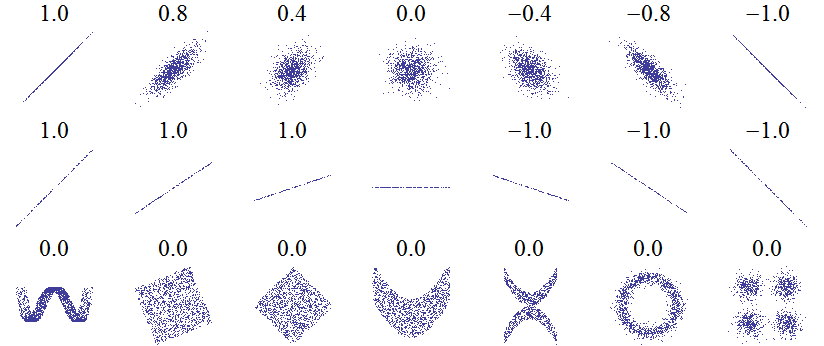
\includegraphics[height=2.5in]{figs/Correlation_examples.png}}
\caption{Examples of datasets with a range of correlations.}
\label{corr_examples}
\end{figure}

Figure~\ref{corr_examples} is from
\url{http://wikipedia.org/wiki/Correlation_and_dependence}.  It shows
scatter plots and correlation coefficients for several
carefully constructed datasets.
\index{scatter plot}
\index{plot!scatter}

The top row shows linear relationships with a range of correlations;
you can use this row to get a sense of what different values of
$\rho$ look like.  The second row shows perfect correlations with a
range of slopes, which demonstrates that correlation is unrelated to
slope (we'll talk about estimating slope soon).  The third row shows
variables that are clearly related, but because the relationship is
nonlinear, the correlation coefficient is 0.
\index{nonlinear}

The moral of this story is that you should always look at a scatter
plot of your data before blindly computing a correlation coefficient.
\index{correlation}


\section{Spearman's rank correlation}

Pearson's correlation works well if the relationship between variables
is linear and if the variables are roughly normal.  But it is not
robust in the presence of outliers.
\index{Pearson coefficient of correlation}
\index{Spearman coefficient of correlation}
\index{normal distribution}
\index{distribution!normal}
\index{Gaussian distribution}
\index{distribution!Gaussian}
\index{robust}
Spearman's rank correlation is an alternative that mitigates the
effect of outliers and skewed distributions.  To compute Spearman's
correlation, we have to compute the {\bf rank} of each value, which is its
index in the sorted sample.  For example, in the sample {\tt [1, 2, 5, 7]}
the rank of the value 5 is 3, because it appears third in the sorted
list.  Then we compute Pearson's correlation for the ranks.
\index{skewness}
\index{outlier}
\index{rank}

{\tt thinkstats2} provides a function that computes Spearman's rank
correlation:

\begin{verbatim}
def SpearmanCorr(xs, ys):
    xranks = pandas.Series(xs).rank()
    yranks = pandas.Series(ys).rank()
    return Corr(xranks, yranks)
\end{verbatim}

I convert the arguments to pandas Series objects so I can use
{\tt rank}, which computes the rank for each value and returns
a Series.  Then I use {\tt Corr} to compute the correlation
of the ranks.
\index{pandas}
\index{Series}

I could also use {\tt Series.corr} directly and specify
Spearman's method:

\begin{verbatim}
def SpearmanCorr(xs, ys):
    xs = pandas.Series(xs)
    ys = pandas.Series(ys)
    return xs.corr(ys, method='spearman')
\end{verbatim}

The Spearman rank correlation for the BRFSS data is 0.54, a little
higher than the Pearson correlation, 0.51.  There are several possible
reasons for the difference, including:
\index{rank correlation}
\index{BRFSS}

\begin{itemize}

\item If the relationship is
nonlinear, Pearson's correlation tends to underestimate the strength
of the relationship, and 
\index{nonlinear}

\item Pearson's correlation can be affected (in either direction)
if one of the distributions is skewed or contains outliers.  Spearman's
rank correlation is more robust.
\index{skewness}
\index{outlier}
\index{robust}

\end{itemize}

In the BRFSS example, we know that the distribution of weights is
roughly lognormal; under a log transform it approximates a normal
distribution, so it has no skew.
So another way to eliminate the effect of skewness is to
compute Pearson's
correlation with log-weight and height:
\index{lognormal distribution}
\index{distribution!lognormal}

\begin{verbatim}
    thinkstats2.Corr(df.htm3, np.log(df.wtkg2)))
\end{verbatim}

The result is 0.53, close to the rank correlation, 0.54.  So that
suggests that skewness in the distribution of weight explains most of
the difference between Pearson's and Spearman's correlation.
\index{skewness}
\index{Spearman coefficient of correlation}
\index{Pearson coefficient of correlation}


\section{Correlation and causation}
\index{correlation}
\index{causation}

If variables A and B are correlated, there are three possible
explanations: A causes B, or B causes A, or some other set of factors
causes both A and B.  These explanations are called ``causal
relationships''.
\index{causal relationship}

Correlation alone does not distinguish between these explanations,
so it does not tell you which ones are true.
This rule is often summarized with the phrase ``Correlation
does not imply causation,'' which is so pithy it has its own
Wikipedia page: \url{http://wikipedia.org/wiki/Correlation_does_not_imply_causation}.

So what can you do to provide evidence of causation?

\begin{enumerate}

\item Use time.  If A comes before B, then A can cause B but not the
  other way around (at least according to our common understanding of
  causation).  The order of events can help us infer the direction
  of causation, but it does not preclude the possibility that something
  else causes both A and B.

\item Use randomness.  If you divide a large sample into two
  groups at random and compute the means of almost any variable, you
  expect the difference to be small.
  If the groups are nearly identical in all variables but one, you
  can eliminate spurious relationships.
  \index{spurious relationship}

  This works even if you don't know what the relevant variables
  are, but it works even better if you do, because you can check that
  the groups are identical.

\end{enumerate}

These ideas are the motivation for the {\bf randomized controlled
trial}, in which subjects are assigned randomly to two (or more)
groups: a {\bf treatment group} that receives some kind of intervention,
like a new medicine, and a {\bf control group} that receives
no intervention, or another treatment whose effects are known.
\index{randomized controlled trial}
\index{controlled trial}
\index{treatment group}
\index{control group}
\index{medicine}

A randomized controlled trial is the most reliable way to demonstrate
a causal relationship, and the foundation of science-based medicine
(see \url{http://wikipedia.org/wiki/Randomized_controlled_trial}).

Unfortunately, controlled trials are only possible in the laboratory
sciences, medicine, and a few other disciplines.  In the social sciences,
controlled experiments are rare, usually because they are impossible
or unethical.
\index{ethics}

An alternative is to look for a {\bf natural experiment}, where
different ``treatments'' are applied to groups that are otherwise
similar.  One danger of natural experiments is that the groups might
differ in ways that are not apparent.  You can read more about this
topic at \url{http://wikipedia.org/wiki/Natural_experiment}.
\index{natural experiment}

In some cases it is possible to infer causal relationships using {\bf
  regression analysis}, which is the topic of Chapter~\ref{regression}.
\index{regression analysis}


\section{Exercises}

A solution to this exercise is in \verb"chap07soln.py".

\begin{exercise}
Using data from the NSFG, make a scatter plot of birth weight
versus mother's age.  Plot percentiles of birth weight
versus mother's age.  Compute Pearson's and Spearman's correlations.
How would you characterize the relationship
between these variables?
\index{birth weight}
\index{weight!birth}
\index{Pearson coefficient of correlation}
\index{Spearman coefficient of correlation}
\end{exercise}


\section{Glossary}

\begin{itemize}

\item scatter plot: A visualization of the relationship between
two variables, showing one point for each row of data.
\index{scatter plot}

\item jitter: Random noise added to data for purposes of
visualization.
\index{jitter}

\item saturation: Loss of information when multiple points are
plotted on top of each other. 
\index{saturation}

\item correlation: A statistic that measures the strength of the
relationship between two variables.
\index{correlation}

\item standardize: To transform a set of values so that their mean is 0 and
their variance is 1.
\index{standardize}

\item standard score: A value that has been standardized so that it is
  expressed in standard deviations from the mean.
  \index{standard score}
\index{standard deviation}

\item covariance: A measure of the tendency of two variables
to vary together.
\index{covariance}

\item rank: The index where an element appears in a sorted list.
\index{rank}

\item randomized controlled trial: An experimental design in which subjects
are divided into groups at random, and different groups are given different
treatments.
\index{randomized controlled trial}

\item treatment group: A group in a controlled trial that receives
some kind of intervention.
\index{treatment group}

\item control group: A group in a controlled trial that receives no
treatment, or a treatment whose effect is known.
\index{control group}

\item natural experiment: An experimental design that takes advantage of
a natural division of subjects into groups in ways that are at least
approximately random.
\index{natural experiment}

\end{itemize}




\chapter{Estimation}
\label{estimation}
\index{estimation}

The code for this chapter is in {\tt estimation.py}.  For information
about downloading and working with this code, see Section~\ref{code}.


\section{The estimation game}

Let's play a game.  I think of a distribution, and you have to guess
what it is.  I'll give you two hints: it's a
normal distribution, and here's a random sample drawn from it:
\index{normal distribution}
\index{distribution!normal}
\index{Gaussian distribution}
\index{distribution!Gaussian}

{\tt [-0.441, 1.774, -0.101, -1.138, 2.975, -2.138]}

What do you think is the mean parameter, $\mu$, of this distribution?
\index{mean}
\index{parameter}

One choice is to use the sample mean, $\xbar$, as an estimate of $\mu$.
In this example, $\xbar$ is 0.155, so it would
be reasonable to guess $\mu$ = 0.155.
This process is called {\bf estimation}, and the statistic we used
(the sample mean) is called an {\bf estimator}.
\index{estimator}

Using the sample mean to estimate $\mu$ is so obvious that it is hard
to imagine a reasonable alternative.  But suppose we change the game by
introducing outliers.
\index{normal distribution}
\index{distribution!normal}
\index{Gaussian distribution}
\index{distribution!Gaussian}

{\em I'm thinking of a distribution.}  It's a normal distribution, and
here's a sample that was collected by an unreliable surveyor who
occasionally puts the decimal point in the wrong place.
\index{measurement error}

{\tt [-0.441, 1.774, -0.101, -1.138, 2.975, -213.8]}

Now what's your estimate of $\mu$?  If you use the sample mean, your
guess is -35.12.  Is that the best choice?  What are the alternatives?
\index{outlier}

One option is to identify and discard outliers, then compute the sample
mean of the rest.  Another option is to use the median as an estimator.
\index{median}

Which estimator is best depends on the circumstances (for example,
whether there are outliers) and on what the goal is.  Are you
trying to minimize errors, or maximize your chance of getting the
right answer?
\index{error}
\index{MSE}
\index{mean squared error}

If there are no outliers, the sample mean minimizes the {\bf mean squared
error} (MSE).  That is, if we play the game many times, and each time
compute the error $\xbar - \mu$, the sample mean minimizes
%
\[ MSE = \frac{1}{m} \sum (\xbar - \mu)^2 \]
%
Where $m$ is the number of times you play the estimation game, not
to be confused with $n$, which is the size of the sample used to
compute $\xbar$.

Here is a function that simulates the estimation game and computes
the root mean squared error (RMSE), which is the square root of
MSE:
\index{mean squared error}
\index{MSE}
\index{RMSE}

\begin{verbatim}
def Estimate1(n=7, m=1000):
    mu = 0
    sigma = 1

    means = []
    medians = []
    for _ in range(m):
        xs = [random.gauss(mu, sigma) for i in range(n)]
        xbar = np.mean(xs)
        median = np.median(xs)
        means.append(xbar)
        medians.append(median)

    print('rmse xbar', RMSE(means, mu))
    print('rmse median', RMSE(medians, mu))
\end{verbatim}

Again, {\tt n} is the size of the sample, and {\tt m} is the
number of times we play the game.  {\tt means} is the list of
estimates based on $\xbar$.  {\tt medians} is the list of medians.
\index{median}

Here's the function that computes RMSE:

\begin{verbatim}
def RMSE(estimates, actual):
    e2 = [(estimate-actual)**2 for estimate in estimates]
    mse = np.mean(e2)
    return math.sqrt(mse)
\end{verbatim}

{\tt estimates} is a list of estimates; {\tt actual} is the
actual value being estimated.  In practice, of course, we don't
know {\tt actual}; if we did, we wouldn't have to estimate it.
The purpose of this experiment is to compare the performance of
the two estimators.
\index{estimator}

When I ran this code, the RMSE of the sample mean was 0.41, which
means that if we use $\xbar$ to estimate the mean of this
distribution, based on a sample with $n=7$, we should expect to be off
by 0.41 on average.  Using the median to estimate the mean yields
RMSE 0.53, which confirms that $\xbar$ yields lower RMSE, at least
for this example.

Minimizing MSE is a nice property, but it's not always the best
strategy.  For example, suppose we are estimating the distribution of
wind speeds at a building site.  If the estimate is too high, we might
overbuild the structure, increasing its cost.  But if it's too
low, the building might collapse.  Because cost as a function of
error is not symmetric, minimizing MSE is not the best strategy.
\index{prediction}
\index{cost function}
\index{MSE}

As another example, suppose I roll three six-sided dice and ask you to
predict the total.  If you get it exactly right, you get a prize;
otherwise you get nothing.  In this case the value that minimizes MSE
is 10.5, but that would be a bad guess, because the total of three
dice is never 10.5.  For this game, you want an estimator that has the
highest chance of being right, which is a {\bf maximum likelihood
  estimator} (MLE).  If you pick 10 or 11, your chance of winning is 1
in 8, and that's the best you can do.  \index{MLE}
\index{maximum likelihood estimator}
\index{dice}


\section{Guess the variance}
\index{variance}
\index{normal distribution}
\index{distribution!normal}
\index{Gaussian distribution}
\index{distribution!Gaussian}

{\em I'm thinking of a distribution.}  It's a normal distribution, and 
here's a (familiar) sample:

{\tt [-0.441, 1.774, -0.101, -1.138, 2.975, -2.138]}

What do you think is the variance, $\sigma^2$, of my distribution?
Again, the obvious choice is to use the sample variance, $S^2$, as an
estimator.
%
\[ S^2 = \frac{1}{n} \sum (x_i - \xbar)^2 \] 
%
For large samples, $S^2$ is an adequate estimator, but for small
samples it tends to be too low.  Because of this unfortunate
property, it is called a {\bf biased} estimator.
An estimator is {\bf unbiased} if the expected total (or mean) error,
after many iterations of the estimation game, is 0.
\index{sample variance}
\index{biased estimator}
\index{estimator!biased}
\index{unbiased estimator}
\index{estimator!unbiased}

Fortunately, there is another simple statistic that is an unbiased
estimator of $\sigma^2$:
%
\[ S_{n-1}^2 = \frac{1}{n-1} \sum (x_i - \xbar)^2 \] 
%
For an explanation of why $S^2$ is biased, and a proof that
$S_{n-1}^2$ is unbiased, see
\url{http://wikipedia.org/wiki/Bias_of_an_estimator}.

The biggest problem with this estimator is that its name and symbol
are used inconsistently.  The name ``sample variance'' can refer to
either $S^2$ or $S_{n-1}^2$, and the symbol $S^2$ is used
for either or both.

Here is a function that simulates the estimation game and tests
the performance of $S^2$ and $S_{n-1}^2$:

\begin{verbatim}
def Estimate2(n=7, m=1000):
    mu = 0
    sigma = 1

    estimates1 = []
    estimates2 = []
    for _ in range(m):
        xs = [random.gauss(mu, sigma) for i in range(n)]
        biased = np.var(xs)
        unbiased = np.var(xs, ddof=1)
        estimates1.append(biased)
        estimates2.append(unbiased)

    print('mean error biased', MeanError(estimates1, sigma**2))
    print('mean error unbiased', MeanError(estimates2, sigma**2))
\end{verbatim}

Again, {\tt n} is the sample size and {\tt m} is the number of times
we play the game.  {\tt np.var} computes $S^2$ by default and
$S_{n-1}^2$ if you provide the argument {\tt ddof=1}, which stands for
``delta degrees of freedom.''  I won't explain that term, but you can read
about it at
\url{http://en.wikipedia.org/wiki/Degrees_of_freedom_(statistics)}.
\index{degrees of freedom}

{\tt MeanError} computes the mean difference between the estimates
and the actual value:

\begin{verbatim}
def MeanError(estimates, actual):
    errors = [estimate-actual for estimate in estimates]
    return np.mean(errors)
\end{verbatim}

When I ran this code, the mean error for $S^2$ was -0.13.  As
expected, this biased estimator tends to be too low.  For $S_{n-1}^2$,
the mean error was 0.014, about 10 times smaller.  As {\tt m}
increases, we expect the mean error for $S_{n-1}^2$ to approach 0.
\index{mean error}

Properties like MSE and bias are long-term expectations based on
many iterations of the estimation game.  By running simulations like
the ones in this chapter, we can compare estimators and check whether
they have desired properties.
\index{biased estimator}
\index{estimator!biased}

But when you apply an estimator to real
data, you just get one estimate.  It would not be meaningful to say
that the estimate is unbiased; being unbiased is a property of the
estimator, not the estimate.

After you choose an estimator with appropriate properties, and use it to
generate an estimate, the next step is to characterize the
uncertainty of the estimate, which is the topic of the next
section.


\section{Sampling distributions}
\label{gorilla}

Suppose you are a scientist studying gorillas in a wildlife
preserve.  You want to know the average weight of the adult
female gorillas in the preserve.  To weigh them, you have
to tranquilize them, which is dangerous, expensive, and possibly
harmful to the gorillas.  But if it is important to obtain this
information, it might be acceptable to weigh a sample of 9
gorillas.  Let's assume that the population of the preserve is
well known, so we can choose a representative sample of adult
females.  We could use the sample mean, $\xbar$, to estimate the
unknown population mean, $\mu$.
\index{gorilla}
\index{population}
\index{sample}

Having weighed 9 female gorillas, you might find $\xbar=90$ kg and
sample standard deviation, $S=7.5$ kg.  The sample mean
is an unbiased estimator of $\mu$, and in the long run it
minimizes MSE.  So if you report a single
estimate that summarizes the results, you would report 90 kg.
\index{MSE}
\index{sample mean}
\index{biased estimator}
\index{estimator!biased}
\index{standard deviation}

But how confident should you be in this estimate?  If you only weigh
$n=9$ gorillas out of a much larger population, you might be unlucky
and choose the 9 heaviest gorillas (or the 9 lightest ones) just by
chance.  Variation in the estimate caused by random selection is
called {\bf sampling error}.
\index{sampling error}

To quantify sampling error, we can simulate the
sampling process with hypothetical values of $\mu$ and $\sigma$, and
see how much $\xbar$ varies.

Since we don't know the actual values of 
$\mu$ and $\sigma$ in the population, we'll use the estimates
$\xbar$ and $S$.
So the question we answer is:
``If the actual values of $\mu$ and $\sigma$ were 90 kg and 7.5 kg,
and we ran the same experiment many times, how much would the
estimated mean, $\xbar$, vary?''

The following function answers that question:

\begin{verbatim}
def SimulateSample(mu=90, sigma=7.5, n=9, m=1000):
    means = []
    for j in range(m):
        xs = np.random.normal(mu, sigma, n)
        xbar = np.mean(xs)
        means.append(xbar)

    cdf = thinkstats2.Cdf(means)
    ci = cdf.Percentile(5), cdf.Percentile(95)
    stderr = RMSE(means, mu)
\end{verbatim}

{\tt mu} and {\tt sigma} are the {\em hypothetical} values of
the parameters.  {\tt n} is the sample size, the number of
gorillas we measured.  {\tt m} is the number of times we run
the simulation.
\index{gorilla}
\index{sample size}
\index{simulation}

\begin{figure}
% estimation.py
\centerline{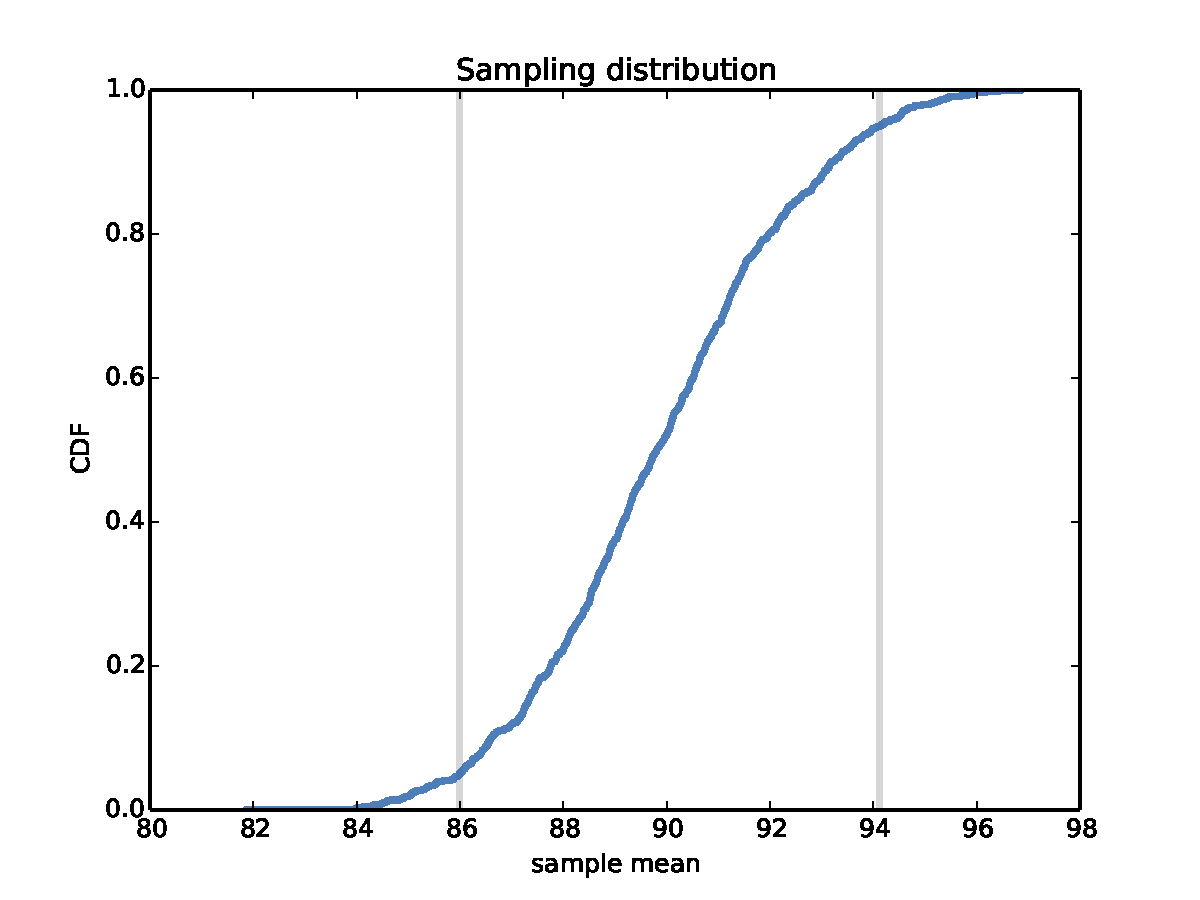
\includegraphics[height=2.5in]{figs/estimation1.pdf}}
\caption{Sampling distribution of $\xbar$, with confidence interval.}
\label{estimation1}
\end{figure}

In each iteration, we choose {\tt n} values from a normal
distribution with the given parameters, and compute the sample mean,
{\tt xbar}.  We run 1000 simulations and then compute the
distribution, {\tt cdf}, of the estimates.  The result is shown in
Figure~\ref{estimation1}.  This distribution is called the {\bf
  sampling distribution} of the estimator.  It shows how much the
estimates would vary if we ran the experiment over and over.
\index{sampling distribution}

The mean of the sampling distribution is pretty close
to the hypothetical value of $\mu$, which means that the experiment
yields the right answer, on average.  After 1000 tries, the lowest
result is 82 kg, and the highest is 98 kg.  This range suggests that
the estimate might be off by as much as 8 kg.

There are two common ways to summarize the sampling distribution:

\begin{itemize}

\item {\bf Standard error} (SE) is a measure of how far we expect the
  estimate to be off, on average.  For each simulated experiment, we
  compute the error, $\xbar - \mu$, and then compute the root mean
  squared error (RMSE).  In this example, it is roughly 2.5 kg.
\index{standard error}

\item A {\bf confidence interval} (CI) is a range that includes a
  given fraction of the sampling distribution.  For example, the 90\%
  confidence interval is the range from the 5th to the 95th
  percentile.  In this example, the 90\% CI is $(86, 94)$ kg.
\index{confidence interval}
\index{sampling distribution}

\end{itemize}

Standard errors and confidence intervals are the source of much confusion:

\begin{itemize}

\item People often confuse standard error and standard deviation.
  Remember that standard deviation describes variability in a measured
  quantity; in this example, the standard deviation of gorilla weight
  is 7.5 kg.  Standard error describes variability in an estimate.  In
  this example, the standard error of the mean, based on a sample of 9
  measurements, is 2.5 kg.
\index{gorilla}
\index{standard deviation}

  One way to remember the difference is that, as sample size
  increases, standard error gets smaller; standard deviation does not.

\item People often think that there is a 90\% probability that the
  actual parameter, $\mu$, falls in the 90\% confidence interval.
  Sadly, that is not true.  If you want to make a claim like that, you
  have to use Bayesian methods (see my book, {\it Think Bayes}).
\index{Bayesian statistics}

  The sampling distribution answers a different question: it gives you
  a sense of how reliable an estimate is by telling you how much it
  would vary if you ran the experiment again.
\index{sampling distribution}

\end{itemize}

It is important to remember that confidence intervals
and standard errors only quantify sampling error; that is,
error due to measuring only part of the population.
The sampling distribution does not account for other
sources of error, notably sampling bias and measurement error, 
which are the topics of the next section.


\section{Sampling bias}

Suppose that instead of the weight of gorillas in a nature preserve,
you want to know the average weight of women in the city where you
live.  It is unlikely that you would be allowed
to choose a representative sample of women and
weigh them.
\index{gorilla}
\index{adult weight}
\index{sampling bias}
\index{bias!sampling}
\index{measurement error}

A simple alternative would be
``telephone sampling;'' that is,
you could choose random numbers from the phone book, call and ask to
speak to an adult woman, and ask how much she weighs.
\index{telephone sampling}
\index{random number}

Telephone sampling has obvious limitations.  For example, the sample
is limited to people whose telephone numbers are listed, so it
eliminates people without phones (who might be poorer than average)
and people with unlisted numbers (who might be richer).  Also, if you
call home telephones during the day, you are less likely to sample
people with jobs.  And if you only sample the person who answers the
phone, you are less likely to sample people who share a phone line.

If factors like income, employment, and household size are related
to weight---and it is plausible that they are---the results of your
survey would be affected one way or another.  This problem is
called {\bf sampling bias} because it is a property of the sampling
process.
\index{sampling bias}

This sampling process is also vulnerable to self-selection, which is a
kind of sampling bias.  Some people will refuse to answer the
question, and if the tendency to refuse is related to weight, that
would affect the results.
\index{self-selection}

Finally, if you ask people how much they weigh, rather than weighing
them, the results might not be accurate.  Even helpful respondents
might round up or down if they are uncomfortable with their actual
weight.  And not all respondents are helpful.  These inaccuracies are
examples of {\bf measurement error}.
\index{measurement error}

When you report an estimated quantity, it is useful to report
standard error, or a confidence interval, or both, in order to
quantify sampling error.  But it is also important to remember that
sampling error is only one source of error, and often it is not the
biggest.
\index{standard error}
\index{confidence interval}


\section{Exponential distributions}
\index{exponential distribution}
\index{distribution!exponential}

Let's play one more round of the estimation game.
{\em I'm thinking of a distribution.}  It's an exponential distribution, and 
here's a sample:

{\tt [5.384, 4.493, 19.198, 2.790, 6.122, 12.844]}

What do you think is the parameter, $\lambda$, of this distribution?
\index{parameter}
\index{mean}

\newcommand{\lamhat}{L}
\newcommand{\lamhatmed}{L_m}

In general, the mean of an exponential distribution is $1/\lambda$,
so working backwards, we might choose
%
\[ \lamhat = 1 / \xbar\]
%
$\lamhat$ is an
estimator of $\lambda$.  And not just any estimator; it is also the
maximum likelihood estimator (see
\url{http://wikipedia.org/wiki/Exponential_distribution#Maximum_likelihood}).
So if you want to maximize your chance of guessing $\lambda$ exactly,
$\lamhat$ is the way to go.
\index{MLE}
\index{maximum likelihood estimator}

But we know that $\xbar$ is not robust in the presence of outliers, so
we expect $\lamhat$ to have the same problem.
\index{robust}
\index{outlier}
\index{sample median}

We can choose an alternative based on the sample median.
The median of an exponential distribution is $\ln(2) / \lambda$,
so working backwards again, we can define an estimator
%
\[ \lamhatmed = \ln(2) / m \]
%
where $m$ is the sample median.
\index{median}

To test the performance of these estimators, we can simulate the
sampling process:

\begin{verbatim}
def Estimate3(n=7, m=1000):
    lam = 2

    means = []
    medians = []
    for _ in range(m):
        xs = np.random.exponential(1.0/lam, n)
        L = 1 / np.mean(xs)
        Lm = math.log(2) / thinkstats2.Median(xs)
        means.append(L)
        medians.append(Lm)

    print('rmse L', RMSE(means, lam))
    print('rmse Lm', RMSE(medians, lam))
    print('mean error L', MeanError(means, lam))
    print('mean error Lm', MeanError(medians, lam))
\end{verbatim}

When I run this experiment with $\lambda=2$, the RMSE of $L$ is
1.1.  For the median-based estimator $L_m$, RMSE is 1.8.  We can't
tell from this experiment whether $L$ minimizes MSE, but at least
it seems better than $L_m$.
\index{MSE}
\index{RMSE}

Sadly, it seems that both estimators are biased.  For $L$ the mean
error is 0.33; for $L_m$ it is 0.45.  And neither converges to 0
as {\tt m} increases.
\index{biased estimator}
\index{estimator!biased}

It turns out that $\xbar$ is an unbiased estimator of the mean
of the distribution, $1 / \lambda$, but $L$ is not an unbiased
estimator of $\lambda$.


\section{Exercises}

For the following exercises, you might want to start with a copy of
{\tt estimation.py}.  Solutions are in \verb"chap08soln.py"

\begin{exercise}

In this chapter we used $\xbar$ and median to estimate $\mu$, and
found that $\xbar$  yields lower MSE.
Also, we used $S^2$ and $S_{n-1}^2$ to estimate $\sigma$, and found that
$S^2$ is biased and $S_{n-1}^2$ unbiased.

Run similar experiments to see if $\xbar$ and median are biased estimates
of $\mu$.
Also check whether $S^2$ or $S_{n-1}^2$ yields a lower MSE.
\index{sample mean}
\index{sample median}
\index{estimator!biased}

\end{exercise}


\begin{exercise}

Suppose you draw a sample with size $n=10$ from 
an exponential distribution with $\lambda=2$.  Simulate
this experiment 1000 times and plot the sampling distribution of
the estimate $\lamhat$.  Compute the standard error of the estimate
and the 90\% confidence interval.
\index{standard error}
\index{confidence interval}
\index{sampling distribution}

Repeat the experiment with a few different values of $n$ and make
a plot of standard error versus $n$.
\index{exponential distribution}
\index{distribution!exponential}


\end{exercise}


\begin{exercise}

In games like hockey and soccer, the time between goals is
roughly exponential.  So you could estimate a team's goal-scoring rate
by observing the number of goals they score in a game.  This
estimation process is a little different from sampling the time
between goals, so let's see how it works.
\index{hockey}
\index{soccer}

Write a function that takes a goal-scoring rate, {\tt lam}, in goals
per game, and simulates a game by generating the time between goals
until the total time exceeds 1 game, then returns the number of goals
scored.

Write another function that simulates many games, stores the
estimates of {\tt lam}, then computes their mean error and RMSE.

Is this way of making an estimate biased?  Plot the sampling
distribution of the estimates and the 90\% confidence interval.  What
is the standard error?  What happens to sampling error for increasing
values of {\tt lam}?
\index{estimator!biased}
\index{biased estimator}
\index{standard error}
\index{confidence interval}

\end{exercise}


\section{Glossary}

\begin{itemize}

\item estimation: The process of inferring the parameters of a distribution
from a sample.
\index{estimation}

\item estimator: A statistic used to estimate a parameter.
\index{estimation}

\item mean squared error (MSE): A measure of estimation error.
\index{mean squared error}
\index{MSE}

\item root mean squared error (RMSE): The square root of MSE,
a more meaningful representation of typical error magnitude.
\index{mean squared error}
\index{MSE}

\item maximum likelihood estimator (MLE): An estimator that computes the
point estimate most likely to be correct.
\index{MLE}
\index{maximum likelihood estimator}

\item bias (of an estimator): The tendency of an estimator to be above or
  below the actual value of the parameter, when averaged over repeated
  experiments.  \index{biased estimator}

\item sampling error: Error in an estimate due to the limited
  size of the sample and variation due to chance. \index{point estimation}

\item sampling bias: Error in an estimate due to a sampling process
  that is not representative of the population. \index{sampling bias}

\item measurement error: Error in an estimate due to inaccuracy collecting
  or recording data. \index{measurement error}

\item sampling distribution: The distribution of a statistic if an
  experiment is repeated many times.  \index{sampling distribution}

\item standard error: The RMSE of an estimate,
which quantifies variability due to sampling error (but not
other sources of error).
\index{standard error}

\item confidence interval: An interval that represents the expected
  range of an estimator if an experiment is repeated many times.
  \index{confidence interval} \index{interval!confidence}

\end{itemize}


\chapter{Hypothesis testing}
\label{testing}

The code for this chapter is in {\tt hypothesis.py}.  For information
about downloading and working with this code, see Section~\ref{code}.

\section{Classical hypothesis testing}
\index{hypothesis testing}
\index{apparent effect}

Exploring the data from the NSFG, we saw several ``apparent effects,''
including differences between first babies and others.
So far we have taken these effects at face value; in this chapter,
we put them to the test.
\index{National Survey of Family Growth}
\index{NSFG}

The fundamental question we want to address is whether the effects
we see in a sample are likely to appear in the larger population.
For example, in the NSFG sample we see a difference in mean pregnancy
length for first babies and others.  We would like to know if
that effect reflects a real difference for women
in the U.S., or if it might appear in the sample by chance.
\index{pregnancy length} \index{length!pregnancy}

There are several ways we could formulate this question, including
Fisher null hypothesis testing, Neyman-Pearson decision theory, and
Bayesian inference\footnote{For more about Bayesian inference, see the
  sequel to this book, {\it Think Bayes}.}.  What I present here is a
subset of all three that makes up most of what people use in practice,
which I will call {\bf classical hypothesis testing}.
\index{Bayesian inference}
\index{null hypothesis}

The goal of classical hypothesis testing is to answer the question,
``Given a sample and an apparent effect, what is the probability of
seeing such an effect by chance?''  Here's how we answer that question:

\begin{itemize}

\item The first step is to quantify the size of the apparent effect by
  choosing a {\bf test statistic}.  In the NSFG example, the apparent
  effect is a difference in pregnancy length between first babies and
  others, so a natural choice for the test statistic is the difference
  in means between the two groups.
  \index{test statistic}

\item The second step is to define a {\bf null hypothesis}, which is a
  model of the system based on the assumption that the apparent effect
  is not real.  In the NSFG example the null hypothesis is that there
  is no difference between first babies and others; that is, that
  pregnancy lengths for both groups have the same distribution.
  \index{null hypothesis}
\index{pregnancy length}
\index{model}

\item The third step is to compute a {\bf p-value}, which is the
  probability of seeing the apparent effect if the null hypothesis is
  true.  In the NSFG example, we would compute the actual difference
  in means, then compute the probability of seeing a
  difference as big, or bigger, under the null hypothesis.
  \index{p-value}

\item The last step is to interpret the result.  If the p-value is
  low, the effect is said to be {\bf statistically significant}, which
  means that it is unlikely to have occurred by chance.  In that case
  we infer that the effect is more likely to appear in the larger
  population.  \index{statistically significant} \index{significant}

\end{itemize}

The logic of this process is similar to a proof by
contradiction.  To prove a mathematical statement, A, you assume
temporarily that A is false.  If that assumption leads to a
contradiction, you conclude that A must actually be true.
\index{contradiction, proof by}
\index{proof by contradiction}

Similarly, to test a hypothesis like, ``This effect is real,'' we
assume, temporarily, that it is not.  That's the null hypothesis.
Based on that assumption, we compute the probability of the apparent
effect.  That's the p-value.  If the p-value is low, we
conclude that the null hypothesis is unlikely to be true.
\index{p-value}
\index{null hypothesis}


\section{HypothesisTest}
\label{hypotest}
\index{mean!difference in}

{\tt thinkstats2} provides {\tt HypothesisTest}, a
class that represents the structure of a classical hypothesis
test.  Here is the definition:
\index{HypothesisTest}

\begin{verbatim}
class HypothesisTest(object):

    def __init__(self, data):
        self.data = data
        self.MakeModel()
        self.actual = self.TestStatistic(data)

    def PValue(self, iters=1000):
        self.test_stats = [self.TestStatistic(self.RunModel()) 
                           for _ in range(iters)]

        count = sum(1 for x in self.test_stats if x >= self.actual)
        return count / iters

    def TestStatistic(self, data):
        raise UnimplementedMethodException()

    def MakeModel(self):
        pass

    def RunModel(self):
        raise UnimplementedMethodException()
\end{verbatim}

{\tt HypothesisTest} is an abstract parent class that provides
complete definitions for some methods and place-keepers for others.
Child classes based on {\tt HypothesisTest} inherit \verb"__init__"
and {\tt PValue} and provide {\tt TestStatistic},
{\tt RunModel}, and optionally {\tt MakeModel}.
\index{HypothesisTest}

\verb"__init__" takes the data in whatever form is appropriate.  It
calls {\tt MakeModel}, which builds a representation of the null
hypothesis, then passes the data to {\tt TestStatistic}, which
computes the size of the effect in the sample.
\index{test statistic}
\index{null hypothesis}

{\tt PValue} computes the probability of the apparent effect under
the null hypothesis.  It takes as a parameter {\tt iters}, which is
the number of simulations to run.  The first line generates simulated
data, computes test statistics, and stores them in
\verb"test_stats".
The result is
the fraction of elements in \verb"test_stats" that
exceed or equal the observed test statistic, {\tt self.actual}.
\index{simulation}

As a simple example\footnote{Adapted from MacKay, {\it Information
    Theory, Inference, and Learning Algorithms}, 2003.}, suppose we
toss a coin 250 times and see 140 heads and 110 tails.  Based on this
result, we might suspect that the coin is biased; that is, more likely
to land heads.  To test this hypothesis, we compute the
probability of seeing such a difference if the coin is actually
fair:
\index{biased coin}
\index{MacKay, David}

\begin{verbatim}
class CoinTest(thinkstats2.HypothesisTest):

    def TestStatistic(self, data):
        heads, tails = data
        test_stat = abs(heads - tails)
        return test_stat

    def RunModel(self):
        heads, tails = self.data
        n = heads + tails
        sample = [random.choice('HT') for _ in range(n)]
        hist = thinkstats2.Hist(sample)
        data = hist['H'], hist['T']
        return data
\end{verbatim}

The parameter, {\tt data}, is a pair of
integers: the number of heads and tails.  The test statistic is
the absolute difference between them, so {\tt self.actual}
is 30.
\index{HypothesisTest}

{\tt RunModel} simulates coin tosses assuming that the coin is
actually fair.  It generates a sample of 250 tosses, uses Hist
to count the number of heads and tails, and returns a pair of
integers.
\index{Hist}
\index{model}

Now all we have to do is instantiate {\tt CoinTest} and call
{\tt PValue}:

\begin{verbatim}
    ct = CoinTest((140, 110))
    pvalue = ct.PValue()
\end{verbatim}

The result is about 0.07, which means that if the coin is
fair, we expect to see a difference as big as 30 about 7\% of the
time.

How should we interpret this result?  By convention,
5\% is the threshold of statistical significance.  If the
p-value is less than 5\%, the effect is considered significant; otherwise
it is not.
\index{p-value}
\index{statistically significant} \index{significant}

But the choice of 5\% is arbitrary, and (as we will see later) the
p-value depends on the choice of the test statistics and
the model of the null hypothesis.  So p-values should not be considered
precise measurements.
\index{null hypothesis}

I recommend interpreting p-values according to their order of
magnitude: if the p-value is less than 1\%, the effect is unlikely to
be due to chance; if it is greater than 10\%, the effect can plausibly
be explained by chance.  P-values between 1\% and 10\% should be
considered borderline.  So in this example I conclude that the
data do not provide strong evidence that the coin is biased or not.


\section{Testing a difference in means}
\label{testdiff}
\index{mean!difference in}

One of the most common effects to test is a difference in mean
between two groups.  In the NSFG data, we saw that the mean pregnancy
length for first babies is slightly longer, and the mean birth weight
is slightly smaller.  Now we will see if those effects are
statistically significant.
\index{National Survey of Family Growth}
\index{NSFG}
\index{pregnancy length}
\index{length!pregnancy}

For these examples, the null hypothesis is that the distributions
for the two groups are the same.  One way to model the null
hypothesis is by {\bf permutation}; that is, we can take values
for first babies and others and shuffle them, treating
the two groups as one big group:
\index{null hypothesis}
\index{permutation}
\index{model}

\begin{verbatim}
class DiffMeansPermute(thinkstats2.HypothesisTest):

    def TestStatistic(self, data):
        group1, group2 = data
        test_stat = abs(group1.mean() - group2.mean())
        return test_stat

    def MakeModel(self):
        group1, group2 = self.data
        self.n, self.m = len(group1), len(group2)
        self.pool = np.hstack((group1, group2))

    def RunModel(self):
        np.random.shuffle(self.pool)
        data = self.pool[:self.n], self.pool[self.n:]
        return data
\end{verbatim}

{\tt data} is a pair of sequences, one for each
group.  The test statistic is the absolute difference in the means.
\index{HypothesisTest}

{\tt MakeModel} records the sizes of the groups, {\tt n} and
{\tt m}, and combines the groups into one NumPy
array, {\tt self.pool}.
\index{NumPy}

{\tt RunModel} simulates the null hypothesis by shuffling the
pooled values and splitting them into two groups with sizes {\tt n}
and {\tt m}.  As always, the return value from {\tt RunModel} has
the same format as the observed data.
\index{null hypothesis}
\index{model}

To test the difference in pregnancy length, we run:

\begin{verbatim}
    live, firsts, others = first.MakeFrames()
    data = firsts.prglngth.values, others.prglngth.values
    ht = DiffMeansPermute(data)
    pvalue = ht.PValue()
\end{verbatim}

{\tt MakeFrames} reads the NSFG data and returns DataFrames
representing all live births, first babies, and others.
We extract pregnancy lengths as NumPy arrays, pass them as
data to {\tt DiffMeansPermute}, and compute the p-value.  The
result is about 0.17, which means that we expect to see a difference
as big as the observed effect about 17\% of the time.  So
this effect is not statistically significant.
\index{DataFrame}
\index{p-value}
  \index{significant} \index{statistically significant}
\index{pregnancy length}

\begin{figure}
% hypothesis.py
\centerline{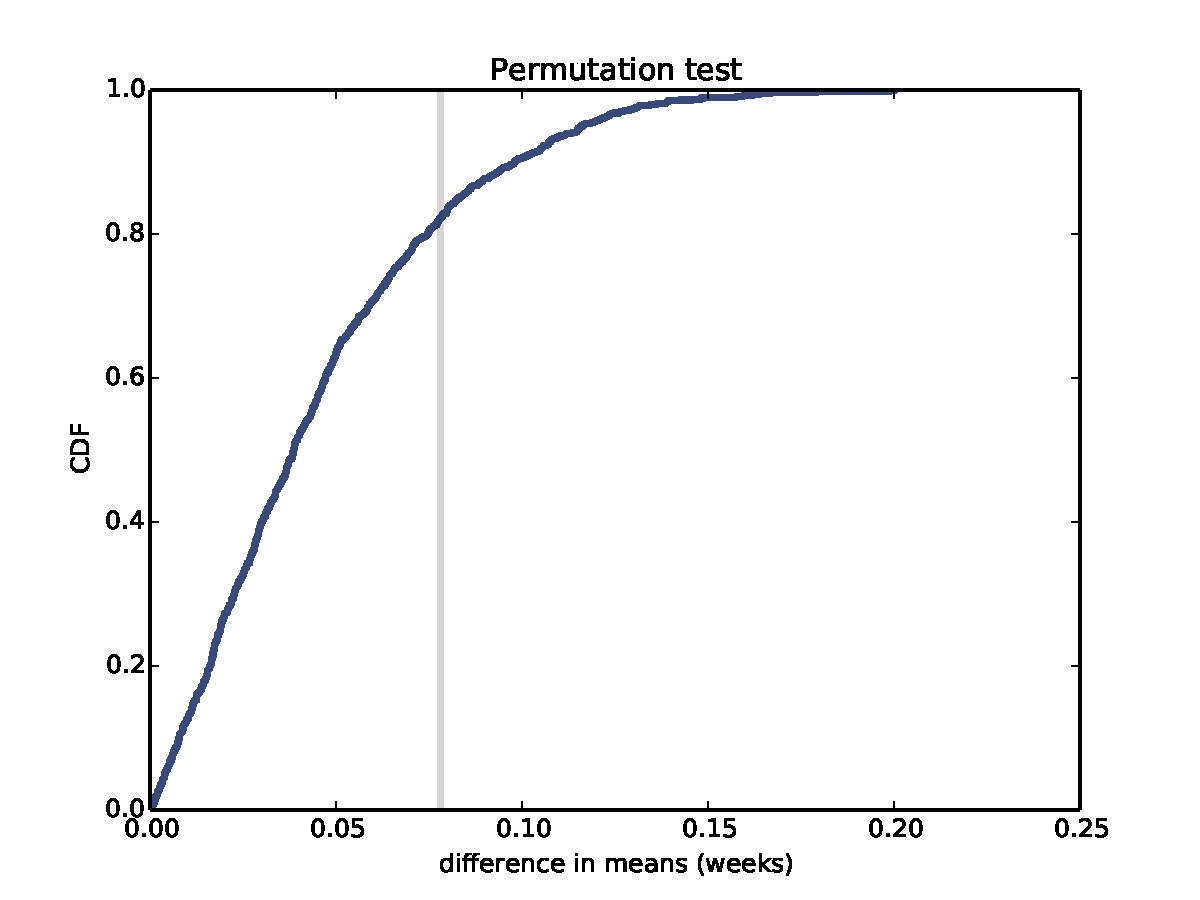
\includegraphics[height=2.5in]{figs/hypothesis1.pdf}}
\caption{CDF of difference in mean pregnancy length under the null
hypothesis.}
\label{hypothesis1}
\end{figure}

{\tt HypothesisTest} provides {\tt PlotCdf}, which plots the
distribution of the test statistic and a gray line indicating
the observed effect size:
\index{thinkplot}
\index{HypothesisTest}
\index{Cdf}
\index{effect size}

\begin{verbatim}
    ht.PlotCdf()
    thinkplot.Show(xlabel='test statistic',
                   ylabel='CDF')
\end{verbatim}

Figure~\ref{hypothesis1} shows the result.  The CDF intersects the
observed difference at 0.83, which is the complement of the p-value,
0.17.
\index{p-value}

If we run the same analysis with birth weight, the computed p-value
is 0; after 1000 attempts,
the simulation never yields an effect
as big as the observed difference, 0.12 lbs.  So we would
report $p < 0.001$, and
conclude that the difference in birth weight is statistically
significant.
\index{birth weight}
\index{weight!birth}
  \index{significant} \index{statistically significant}


\section{Other test statistics}

Choosing the best test statistic depends on what question you are
trying to address.  For example, if the relevant question is whether
pregnancy lengths are different for first
babies, then it makes sense to test the absolute difference in means,
as we did in the previous section.
\index{test statistic}
\index{pregnancy length}

If we had some reason to think that first babies are likely
to be late, then we would not take the absolute value of the difference;
instead we would use this test statistic:

\begin{verbatim}
class DiffMeansOneSided(DiffMeansPermute):

    def TestStatistic(self, data):
        group1, group2 = data
        test_stat = group1.mean() - group2.mean()
        return test_stat
\end{verbatim}

{\tt DiffMeansOneSided} inherits {\tt MakeModel} and {\tt RunModel}
from {\tt DiffMeansPermute}; the only difference is that
{\tt TestStatistic} does not take the absolute value of the
difference.  This kind of test is called {\bf one-sided} because
it only counts one side of the distribution of differences.  The
previous test, using both sides, is {\bf two-sided}.
\index{one-sided test}
\index{two-sided test}

For this version of the test, the p-value is 0.09.  In general
the p-value for a one-sided test is about half the p-value for
a two-sided test, depending on the shape of the distribution.
\index{p-value}

The one-sided hypothesis, that first babies are born late, is more
specific than the two-sided hypothesis, so the p-value is smaller.
But even for the stronger hypothesis, the difference is
not statistically significant.
  \index{significant} \index{statistically significant}

We can use the same framework to test for a difference in standard
deviation.  In Section~\ref{visualization}, we saw some evidence that
first babies are more likely to be early or late, and less likely to
be on time.  So we might hypothesize that the standard deviation is
higher.  Here's how we can test that:
\index{standard deviation}

\begin{verbatim}
class DiffStdPermute(DiffMeansPermute):

    def TestStatistic(self, data):
        group1, group2 = data
        test_stat = group1.std() - group2.std()
        return test_stat
\end{verbatim}

This is a one-sided test because the hypothesis is that the standard
deviation for first babies is higher, not just different.  The p-value
is 0.09, which is not statistically significant.
\index{p-value}
\index{permutation}
  \index{significant} \index{statistically significant}


\section{Testing a correlation}
\label{corrtest}

This framework can also test correlations.  For example, in the NSFG
data set, the correlation between birth weight and mother's age is
about 0.07.  It seems like older mothers have heavier babies.  But
could this effect be due to chance?
\index{correlation}
\index{test statistic}

For the test statistic, I use
Pearson's correlation, but Spearman's would work as well.
If we had reason to expect positive correlation, we would do a
one-sided test.  But since we have no such reason, I'll
do a two-sided test using the absolute value of correlation.
\index{Pearson coefficient of correlation}
\index{Spearman coefficient of correlation}

The null hypothesis is that there is no correlation between mother's
age and birth weight.  By shuffling the observed values, we can
simulate a world where the distributions of age and
birth weight are the same, but where the variables are unrelated:
\index{birth weight}
\index{weight!birth}
\index{null hypothesis}

\begin{verbatim}
class CorrelationPermute(thinkstats2.HypothesisTest):

    def TestStatistic(self, data):
        xs, ys = data
        test_stat = abs(thinkstats2.Corr(xs, ys))
        return test_stat

    def RunModel(self):
        xs, ys = self.data
        xs = np.random.permutation(xs)
        return xs, ys
\end{verbatim}

{\tt data} is a pair of sequences.  {\tt TestStatistic} computes the
absolute value of Pearson's correlation.  {\tt RunModel} shuffles the
{\tt xs} and returns simulated data.
\index{HypothesisTest}
\index{permutation}
\index{Pearson coefficient of correlation}

Here's the code that reads the data and runs the test:

\begin{verbatim}
    live, firsts, others = first.MakeFrames()
    live = live.dropna(subset=['agepreg', 'totalwgt_lb'])
    data = live.agepreg.values, live.totalwgt_lb.values
    ht = CorrelationPermute(data)
    pvalue = ht.PValue()
\end{verbatim}

I use {\tt dropna} with the {\tt subset} argument to drop rows
that are missing either of the variables we need.
\index{dropna}
\index{NaN}
\index{missing values}

The actual correlation is 0.07.  The computed p-value is 0; after 1000
iterations the largest simulated correlation is 0.04.  So although the
observed correlation is small, it is statistically significant.
\index{p-value}
  \index{significant} \index{statistically significant}

This example is a reminder that ``statistically significant'' does not
always mean that an effect is important, or significant in practice.
It only means that it is unlikely to have occurred by chance.


\section{Testing proportions}
\label{casino}
\index{chi-squared test}

Suppose you run a casino and you suspect that a customer is
using a crooked die; that
is, one that has been modified to make one of the faces more
likely than the others.  You apprehend the alleged
cheater and confiscate the die, but now you have to prove that it
is crooked.  You roll the die 60 times and get the following results:
\index{casino}
\index{dice}
\index{crooked die}

\begin{center}
\begin{tabular}{|l|c|c|c|c|c|c|}
\hline
Value     &  1  &  2  &  3  &  4  &  5  &  6  \\ 
\hline
Frequency &  8  &  9  &  19  &  5  &  8  &  11  \\
\hline
\end{tabular}
\end{center}

On average you expect each value to appear 10 times.  In this
dataset, the value 3 appears more often than expected, and the value 4
appears less often.  But are these differences statistically
significant?
\index{frequency}
  \index{significant} \index{statistically significant}

To test this hypothesis, we can compute the expected frequency for
each value, the difference between the expected and observed
frequencies, and the total absolute difference.  In this
example, we expect each side to come up 10 times out of 60; the
deviations from this expectation are -2, -1, 9, -5, -2, and 1; so the
total absolute difference is 20.  How often would we see such a
difference by chance?
\index{deviation}

Here's a version of {\tt HypothesisTest} that answers that question:
\index{HypothesisTest}

\begin{verbatim}
class DiceTest(thinkstats2.HypothesisTest):

    def TestStatistic(self, data):
        observed = data
        n = sum(observed)
        expected = np.ones(6) * n / 6
        test_stat = sum(abs(observed - expected))
        return test_stat

    def RunModel(self):
        n = sum(self.data)
        values = [1, 2, 3, 4, 5, 6]
        rolls = np.random.choice(values, n, replace=True)
        hist = thinkstats2.Hist(rolls)
        freqs = hist.Freqs(values)
        return freqs
\end{verbatim}

The data are represented as a list of frequencies: the observed
values are {\tt [8, 9, 19, 5, 8, 11]}; the expected frequencies
are all 10.  The test statistic is the sum of the absolute differences.
\index{frequency}

The null hypothesis is that the die is fair, so we simulate that by
drawing random samples from {\tt values}.  {\tt RunModel} uses {\tt
  Hist} to compute and return the list of frequencies.
\index{Hist}
\index{null hypothesis}
\index{model}

The p-value for this data is 0.13, which means that if the die is
fair we expect to see the observed total deviation, or more, about
13\% of the time.  So the apparent effect is not statistically
significant.
\index{p-value}
\index{deviation}
  \index{significant} \index{statistically significant}


\section{Chi-squared tests}
\label{casino2}

In the previous section we used total deviation as the test statistic.
But for testing proportions it is more common to use the chi-squared
statistic:
%
\[ \goodchi^2 = \sum_i \frac{(O_i - E_i)^2}{E_i} \]
%
%% TODO: Consider using upper case chi, which is more strictly correct,
%% but harder to distinguish from X.
% 
Where $O_i$ are the observed frequencies and $E_i$ are the expected
frequencies.  Here's the Python code:
\index{chi-squared test}
\index{chi-squared statistic}
\index{test statistic}

\begin{verbatim}
class DiceChiTest(DiceTest):

    def TestStatistic(self, data):
        observed = data
        n = sum(observed)
        expected = np.ones(6) * n / 6
        test_stat = sum((observed - expected)**2 / expected)
        return test_stat
\end{verbatim}

Squaring the deviations (rather than taking absolute values) gives
more weight to large deviations.  Dividing through by {\tt expected}
standardizes the deviations, although in this case it has no effect
because the expected frequencies are all equal.
\index{deviation}

The p-value using the chi-squared statistic is 0.04,
substantially smaller than what we got using total deviation, 0.13.
If we take the 5\% threshold seriously, we would consider this effect
statistically significant.  But considering the two tests togther, I
would say that the results are borderline.  I would not rule out the
possibility that the die is crooked, but I would not convict the
accused cheater.
\index{p-value}
  \index{significant} \index{statistically significant}

This example demonstrates an important point: the p-value depends
on the choice of test statistic and the model of the null hypothesis,
and sometimes these choices determine whether an effect is
statistically significant or not.
\index{null hypothesis}
\index{model}


\section{First babies again}

Earlier in this chapter we looked at pregnancy lengths for first
babies and others, and concluded that the apparent differences in
mean and standard deviation are not statistically significant.  But in
Section~\ref{visualization}, we saw several apparent differences
in the distribution of pregnancy length, especially in the range from
35 to 43 weeks.  To see whether those differences are statistically
significant, we can use a test based on a chi-squared statistic.
\index{standard deviation}
\index{statistically significant} \index{significant}
\index{pregnancy length}

The code combines elements from previous examples:
\index{HypothesisTest}

\begin{verbatim}
class PregLengthTest(thinkstats2.HypothesisTest):

    def MakeModel(self):
        firsts, others = self.data
        self.n = len(firsts)
        self.pool = np.hstack((firsts, others))

        pmf = thinkstats2.Pmf(self.pool)
        self.values = range(35, 44)
        self.expected_probs = np.array(pmf.Probs(self.values))

    def RunModel(self):
        np.random.shuffle(self.pool)
        data = self.pool[:self.n], self.pool[self.n:]
        return data
\end{verbatim}

The data are represented as two lists of pregnancy lengths.  The null
hypothesis is that both samples are drawn from the same distribution.
{\tt MakeModel} models that distribution by pooling the two
samples using {\tt hstack}.  Then {\tt RunModel} generates
simulated data by shuffling the pooled sample and splitting it
into two parts.
\index{null hypothesis}
\index{model}
\index{hstack}
\index{pregnancy length}

{\tt MakeModel} also defines {\tt values}, which is the
range of weeks we'll use, and \verb"expected_probs",
which is the probability of each value in the pooled distribution.

Here's the code that computes the test statistic:

\begin{verbatim}
# class PregLengthTest:

    def TestStatistic(self, data):
        firsts, others = data
        stat = self.ChiSquared(firsts) + self.ChiSquared(others)
        return stat

    def ChiSquared(self, lengths):
        hist = thinkstats2.Hist(lengths)
        observed = np.array(hist.Freqs(self.values))
        expected = self.expected_probs * len(lengths)
        stat = sum((observed - expected)**2 / expected)
        return stat
\end{verbatim}

{\tt TestStatistic} computes the chi-squared statistic for
first babies and others, and adds them.
\index{chi-squared statistic}

{\tt ChiSquared} takes a sequence of pregnancy lengths, computes
its histogram, and computes {\tt observed}, which is a list of
frequencies corresponding to {\tt self.values}.
To compute the list of expected frequencies, it multiplies the
pre-computed probabilities, \verb"expected_probs", by the sample
size.  It returns the chi-squared statistic, {\tt stat}.

For the NSFG data the total chi-squared statistic is 102, which
doesn't mean much by itself.  But after 1000 iterations, the largest
test statistic generated under the null hypothesis is 32.  We conclude
that the observed chi-squared statistic is unlikely under the null
hypothesis, so the apparent effect is statistically significant.
\index{null hypothesis}
\index{statistically significant} \index{significant}

This example demonstrates a limitation of chi-squared tests: they
indicate that there is a difference between the two groups,
but they don't say anything specific about what the difference is.


\section{Errors}
\index{error}

In classical hypothesis testing, an effect is considered statistically
significant if the p-value is below some threshold, commonly 5\%.
This procedure raises two questions:
\index{p-value}
\index{threshold}
\index{statistically significant} \index{significant}

\begin{itemize}

\item If the effect is actually due to chance, what is the probability
that we will wrongly consider it significant?  This
probability is the {\bf false positive rate}.
\index{false positive}

\item If the effect is real, what is the chance that the hypothesis
test will fail?  This probability is the {\bf false negative rate}.
\index{false negative}

\end{itemize}

The false positive rate is relatively easy to compute: if the
threshold is 5\%, the false positive rate is 5\%.  Here's why:

\begin{itemize}

\item If there is no real effect, the null hypothesis is true, so we
  can compute the distribution of the test statistic by simulating the
  null hypothesis.  Call this distribution $\CDF_T$.
\index{null hypothesis}
\index{CDF}

\item Each time we run an experiment, we get a test statistic, $t$,
  which is drawn from $CDF_T$.  Then we compute a p-value, which is
  the probability that a random value from $CDF_T$ exceeds {\tt t},
  so that's $1 - CDF_T(t)$.

\item The p-value is less than 5\% if $CDF_T(t)$ is greater
  than 95\%; that is, if $t$ exceeds the 95th percentile.
  And how often does a value chosen from $CDF_T$ exceed
  the 95th percentile?  5\% of the time.

\end{itemize}

So if you perform one hypothesis test with a 5\% threshold, you expect
a false positive 1 time in 20.


\section{Power}
\label{power}

The false negative rate is harder to compute because it depends on
the actual effect size, and normally we don't know that.
One option is to compute a rate
conditioned on a hypothetical effect size.
\index{effect size}

For example, if we assume that the observed difference between groups
is accurate, we can use the observed samples as a model of the
population and run hypothesis tests with simulated data:
\index{model}

\begin{verbatim}
def FalseNegRate(data, num_runs=100):
    group1, group2 = data
    count = 0

    for i in range(num_runs):
        sample1 = thinkstats2.Resample(group1)
        sample2 = thinkstats2.Resample(group2)

        ht = DiffMeansPermute((sample1, sample2))
        pvalue = ht.PValue(iters=101)
        if pvalue > 0.05:
            count += 1

    return count / num_runs
\end{verbatim}

{\tt FalseNegRate} takes data in the form of two sequences, one for
each group.  Each time through the loop, it simulates an experiment by
drawing a random sample from each group and running a hypothesis test.
Then it checks the result and counts the number of false negatives.
\index{Resample}
\index{permutation}

{\tt Resample} takes a sequence and draws a sample with the same
length, with replacement:
\index{replacement}

\begin{verbatim}
def Resample(xs):
    return np.random.choice(xs, len(xs), replace=True)
\end{verbatim}

Here's the code that tests pregnancy lengths:

\begin{verbatim}
    live, firsts, others = first.MakeFrames()
    data = firsts.prglngth.values, others.prglngth.values
    neg_rate = FalseNegRate(data)
\end{verbatim}

The result is about 70\%, which means that if the actual difference in
mean pregnancy length is 0.078 weeks, we expect an experiment with this
sample size to yield a negative test 70\% of the time.
\index{pregnancy length}

This result is often presented the other way around: if the actual
difference is 0.078 weeks, we should expect a positive test only 30\%
of the time.  This ``correct positive rate'' is called the {\bf power}
of the test, or sometimes ``sensitivity''.  It reflects the ability of
the test to detect an effect of a given size.
\index{power}
\index{sensitivity}
\index{correct positive}

In this example, the test had only a 30\% chance of yielding a
positive result (again, assuming that the difference is 0.078 weeks).
As a rule of thumb, a power of 80\% is considered acceptable, so
we would say that this test was ``underpowered.''
\index{underpowered}

In general a negative hypothesis test does not imply that there is no
difference between the groups; instead it suggests that if there is a
difference, it is too small to detect with this sample size.


\section{Replication}
\label{replication}

The hypothesis testing process I demonstrated in this chapter is not,
strictly speaking, good practice.

First, I performed multiple tests.  If you run one hypothesis test,
the chance of a false positive is about 1 in 20, which might be
acceptable.  But if you run 20 tests, you should expect at least one
false positive, most of the time.
\index{multiple tests}

Second, I used the same dataset for exploration and testing.  If
you explore a large dataset, find a surprising effect, and then test
whether it is significant, you have a good chance of generating a
false positive.
\index{statistically significant} \index{significant}

To compensate for multiple tests, you can adjust the p-value
threshold (see
  \url{https://en.wikipedia.org/wiki/Holm-Bonferroni_method}).  Or you
can address both problems by partitioning the data, using one set for
exploration and the other for testing.
\index{p-value}
\index{Holm-Bonferroni method}

In some fields these practices are required or at least encouraged.
But it is also common to address these problems implicitly by
replicating published results.  Typically the first paper to report a
new result is considered exploratory.  Subsequent papers that
replicate the result with new data are considered confirmatory.
\index{confirmatory result}

As it happens, we have an opportunity to replicate the results in this
chapter.  The first edition of this book is based on Cycle 6 of the
NSFG, which was released in 2002.  In October 2011, the CDC released
additional data based on interviews conducted from 2006--2010.  {\tt
  nsfg2.py} contains code to read and clean this data.  In the new
dataset:
\index{NSFG}

\begin{itemize}

\item The difference in mean pregnancy length is
0.16 weeks and statistically significant with $p < 0.001$ (compared
to 0.078 weeks in the original dataset).
\index{statistically significant} \index{significant}
\index{pregnancy length}

\item The difference in birth weight is 0.17 pounds with $p < 0.001$
(compared to 0.12 lbs in the original dataset).
\index{birth weight}
\index{weight!birth}

\item The correlation between birth weight and mother's age is
0.08 with $p < 0.001$ (compared to 0.07).

\item The chi-squared test is statistically significant with
$p < 0.001$ (as it was in the original).

\end{itemize}

In summary, all of the effects that were statistically significant
in the original dataset were replicated in the new dataset, and the
difference in pregnancy length, which was not significant in the
original, is bigger in the new dataset and significant.


\section{Exercises}

A solution to these exercises is in \verb"chap09soln.py".

\begin{exercise}
As sample size increases, the power of a hypothesis test increases,
which means it is more likely to be positive if the effect is real.
Conversely, as sample size decreases, the test is less likely to
be positive even if the effect is real.
\index{sample size}

To investigate this behavior, run the tests in this chapter with
different subsets of the NSFG data.  You can use {\tt thinkstats2.SampleRows}
to select a random subset of the rows in a DataFrame.
\index{National Survey of Family Growth}
\index{NSFG}
\index{DataFrame}

What happens to the p-values of these tests as sample size decreases?
What is the smallest sample size that yields a positive test?
\index{p-value}
\end{exercise}



\begin{exercise}

In Section~\ref{testdiff}, we simulated the null hypothesis by
permutation; that is, we treated the observed values as if they
represented the entire population, and randomly assigned the
members of the population to the two groups.
\index{null hypothesis}
\index{permutation}

An alternative is to use the sample to estimate the distribution for
the population, then draw a random sample from that distribution.
This process is called {\bf resampling}.  There are several ways to
implement resampling, but one of the simplest is to draw a sample
with replacement from the observed values, as in Section~\ref{power}.
\index{resampling}
\index{replacement}

Write a class named {\tt DiffMeansResample} that inherits from
{\tt DiffMeansPermute} and overrides {\tt RunModel} to implement
resampling, rather than permutation.
\index{permutation}

Use this model to test the differences in pregnancy length and
birth weight.  How much does the model affect the results?
\index{model}
\index{birth weight}
\index{weight!birth}
\index{pregnancy length}

\end{exercise}


\section{Glossary}

\begin{itemize}

\item hypothesis testing: The process of determining whether an apparent
effect is statistically significant.
\index{hypothesis testing}

\item test statistic: A statistic used to quantify an effect size.
\index{test statistic}
\index{effect size}

\item null hypothesis: A model of a system based on the assumption that
an apparent effect is due to chance.
\index{null hypothesis}

\item p-value: The probability that an effect could occur by chance.
\index{p-value}

\item statistically significant: An effect is statistically
  significant if it is unlikely to occur by chance.
  \index{significant} \index{statistically significant}

\item permutation test: A way to compute p-values by generating
  permutations of an observed dataset.
  \index{permutation test}

\item resampling test: A way to compute p-values by generating
  samples, with replacement, from an observed dataset.
  \index{resampling test}

\item two-sided test: A test that asks, ``What is the chance of an effect
as big as the observed effect, positive or negative?''

\item one-sided test: A test that asks, ``What is the chance of an effect
as big as the observed effect, and with the same sign?''
\index{one-sided test}
\index{two-sided test}
\index{test!one-sided}
\index{test!two-sided}

\item chi-squared test: A test that uses the chi-squared statistic as
the test statistic.
\index{chi-squared test}

\item false positive: The conclusion that an effect is real when it is not.
\index{false positive}

\item false negative: The conclusion that an effect is due to chance when it
is not.
\index{false negative}

\item power: The probability of a positive test if the null hypothesis
is false.
\index{power}
\index{null hypothesis}

\end{itemize}


\chapter{Linear least squares}
\label{linear}

The code for this chapter is in {\tt linear.py}.  For information
about downloading and working with this code, see Section~\ref{code}.


\section{Least squares fit}

Correlation coefficients measure the strength and sign of a
relationship, but not the slope.  There are several ways to estimate
the slope; the most common is a {\bf linear least squares fit}.  A
``linear fit'' is a line intended to model the relationship between
variables.  A ``least squares'' fit is one that minimizes the mean
squared error (MSE) between the line and the data.
\index{least squares fit}
\index{linear least squares}
\index{model}

Suppose we have a sequence of points, {\tt ys}, that we want to
express as a function of another sequence {\tt xs}.  If there is a
linear relationship between {\tt xs} and {\tt ys} with intercept {\tt
  inter} and slope {\tt slope}, we expect each {\tt y[i]} to be
{\tt inter + slope * x[i]}.  \index{residuals}

But unless the correlation is perfect, this prediction is only
approximate.  The vertical deviation from the line, or {\bf residual},
is
\index{deviation}

\begin{verbatim}
res = ys - (inter + slope * xs)
\end{verbatim}

The residuals might be due to random factors like measurement error,
or non-random factors that are unknown.  For example, if we are
trying to predict weight as a function of height, unknown factors
might include diet, exercise, and body type.
\index{slope}
\index{intercept}
\index{measurement error}

If we get the parameters {\tt inter} and {\tt slope} wrong, the residuals
get bigger, so it makes intuitive sense that the parameters we want
are the ones that minimize the residuals.
\index{parameter}

We might try to minimize the absolute value of the
residuals, or their squares, or their cubes; but the most common
choice is to minimize the sum of squared residuals,
{\tt sum(res**2))}.

Why?  There are three good reasons and one less important one:

\begin{itemize}

\item Squaring has the feature of treating positive and
negative residuals the same, which is usually what we want.

\item Squaring gives more weight to large residuals, but not
so much weight that the largest residual always dominates.

\item If the residuals are uncorrelated and normally distributed with
  mean 0 and constant (but unknown) variance, then the least squares
  fit is also the maximum likelihood estimator of {\tt inter} and {\tt
    slope}.  See
  \url{https://en.wikipedia.org/wiki/Linear_regression}.  \index{MLE}
  \index{maximum likelihood estimator}
\index{correlation}

\item The values of {\tt inter} and {\tt slope} that minimize
  the squared residuals can be computed efficiently.

\end{itemize}

The last reason made sense when computational efficiency was more
important than choosing the method most appropriate to the problem
at hand.  That's no longer the case, so it is worth considering
whether squared residuals are the right thing to minimize.
\index{computational methods}
\index{squared residuals}

For example, if you are using {\tt xs} to predict values of {\tt ys},
guessing too high might be better (or worse) than guessing too low.
In that case you might want to compute some cost function for each
residual, and minimize total cost, {\tt sum(cost(res))}.
However, computing a least squares fit is quick, easy and often good
enough.  
\index{cost function}


\section{Implementation}

{\tt thinkstats2} provides simple functions that demonstrate
linear least squares:
\index{LeastSquares}

\begin{verbatim}
def LeastSquares(xs, ys):
    meanx, varx = MeanVar(xs)
    meany = Mean(ys)

    slope = Cov(xs, ys, meanx, meany) / varx
    inter = meany - slope * meanx

    return inter, slope
\end{verbatim}

{\tt LeastSquares} takes sequences
{\tt xs} and {\tt ys} and returns the estimated parameters {\tt inter}
and {\tt slope}.
For details on how it works, see
\url{http://wikipedia.org/wiki/Numerical_methods_for_linear_least_squares}.
\index{parameter}

{\tt thinkstats2} also provides {\tt FitLine}, which takes {\tt inter}
and {\tt slope} and returns the fitted line for a sequence
of {\tt xs}.
\index{FitLine}

\begin{verbatim}
def FitLine(xs, inter, slope):
    fit_xs = np.sort(xs)
    fit_ys = inter + slope * fit_xs
    return fit_xs, fit_ys
\end{verbatim}

We can use these functions to compute the least squares fit for
birth weight as a function of mother's age.
\index{birth weight}
\index{weight!birth}
\index{age}

\begin{verbatim}
    live, firsts, others = first.MakeFrames()
    live = live.dropna(subset=['agepreg', 'totalwgt_lb'])
    ages = live.agepreg
    weights = live.totalwgt_lb

    inter, slope = thinkstats2.LeastSquares(ages, weights)
    fit_xs, fit_ys = thinkstats2.FitLine(ages, inter, slope)
\end{verbatim}

The estimated intercept and slope are 6.8 lbs and 0.017 lbs per year.
These values are hard to interpret in this form: the intercept is
the expected weight of a baby whose mother is 0 years old, which
doesn't make sense in context, and the slope is too small to
grasp easily.
\index{slope}
\index{intercept}
\index{dropna}
\index{NaN}

Instead of presenting the intercept at $x=0$, it
is often helpful to present the intercept at the mean of $x$.  In
this case the mean age is about 25 years and the mean baby weight
for a 25 year old mother is 7.3 pounds.  The slope is 0.27 ounces
per year, or 0.17 pounds per decade.

\begin{figure}
% linear.py
\centerline{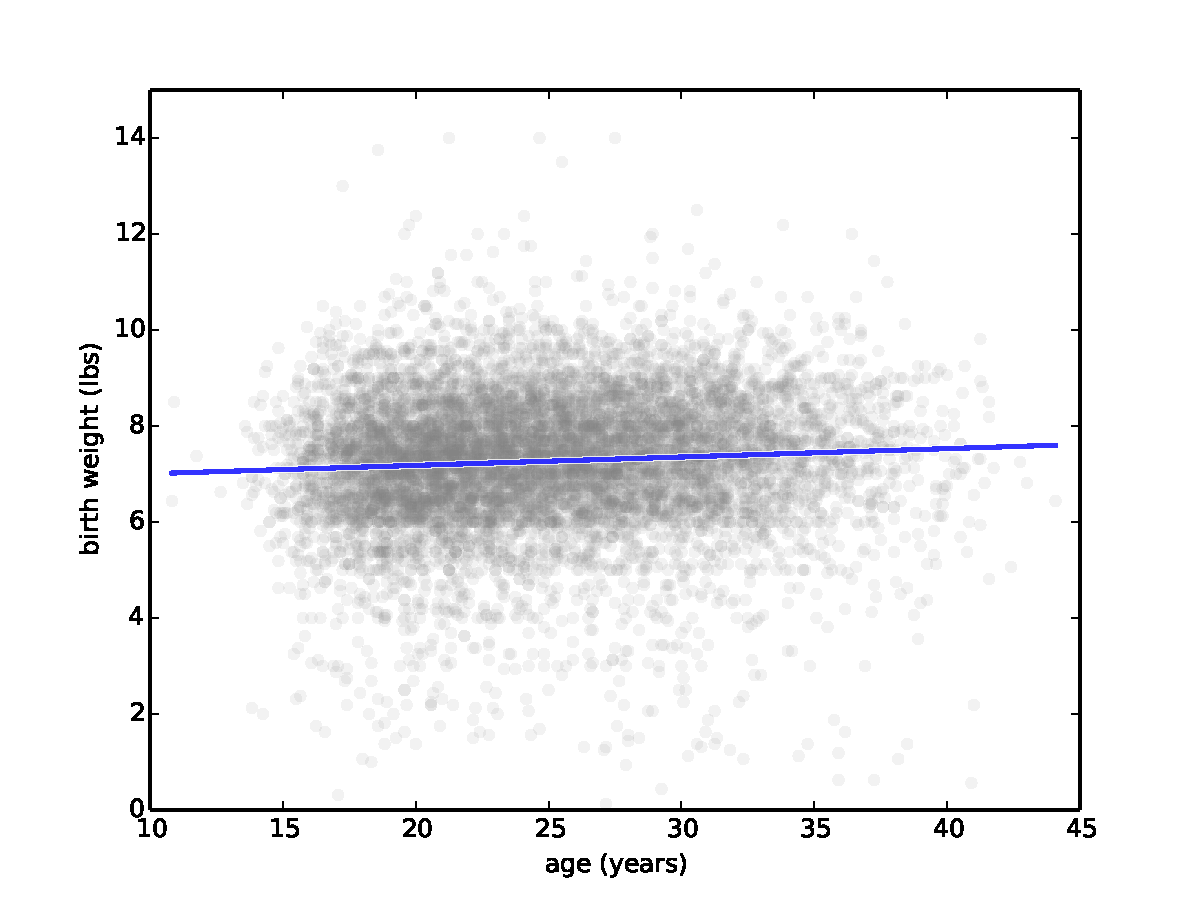
\includegraphics[height=2.5in]{figs/linear1.pdf}}
\caption{Scatter plot of birth weight and mother's age with
a linear fit.}
\label{linear1}
\end{figure}

Figure~\ref{linear1} shows a scatter plot of birth weight and age
along with the fitted line.  It's a good idea to look at a figure like
this to assess whether the relationship is linear and whether the
fitted line seems like a good model of the relationship.
\index{birth weight}
\index{weight!birth}
\index{scatter plot}
\index{plot!scatter}
\index{model}


\section{Residuals}
\label{residuals}

Another useful test is to plot the residuals.
{\tt thinkstats2} provides a function that computes residuals:
\index{residuals}

\begin{verbatim}
def Residuals(xs, ys, inter, slope):
    xs = np.asarray(xs)
    ys = np.asarray(ys)
    res = ys - (inter + slope * xs)
    return res
\end{verbatim}

{\tt Residuals} takes sequences {\tt xs} and {\tt ys} and
estimated parameters {\tt inter} and {\tt slope}.  It returns
the differences between the actual values and the fitted line.

\begin{figure}
% linear.py
\centerline{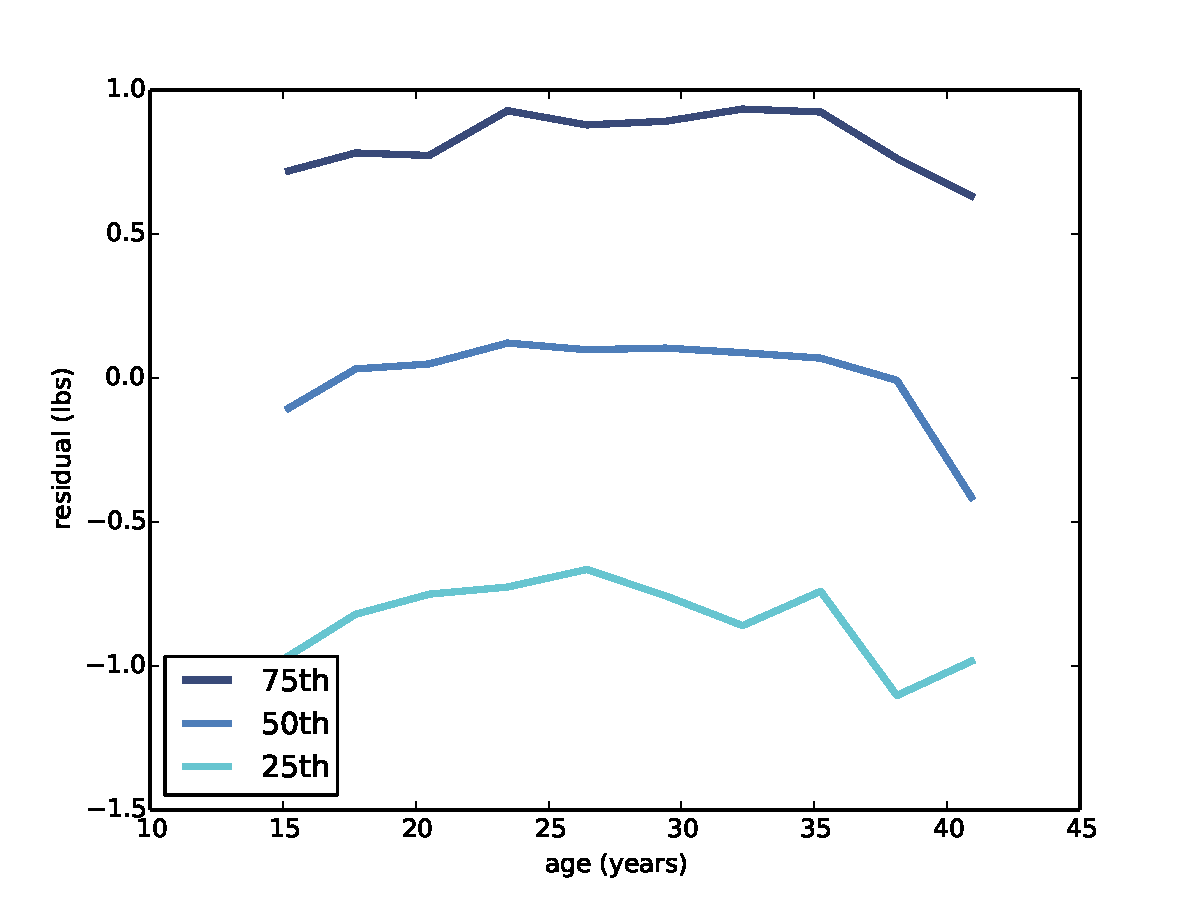
\includegraphics[height=2.5in]{figs/linear2.pdf}}
\caption{Residuals of the linear fit.}
\label{linear2}
\end{figure}

To visualize the residuals, I group respondents by age and compute
percentiles in each group, as we saw in Section~\ref{characterizing}.
Figure~\ref{linear2} shows the 25th, 50th and 75th percentiles of
the residuals for each age group.  The median is near zero, as
expected, and the interquartile range is about 2 pounds.  So if we
know the mother's age, we can guess the baby's weight within a pound,
about 50\% of the time.
\index{visualization}

Ideally these lines should be flat, indicating that the residuals are
random, and parallel, indicating that the variance of the residuals is
the same for all age groups.  In fact, the lines are close to
parallel, so that's good; but they have some curvature, indicating
that the relationship is nonlinear.  Nevertheless, the linear fit
is a simple model that is probably good enough for some purposes.
\index{model}
\index{nonlinear}


\section{Estimation}
\label{regest}

The parameters {\tt slope} and {\tt inter} are estimates based on a
sample; like other estimates, they are vulnerable to sampling bias,
measurement error, and sampling error.  As discussed in
Chapter~\ref{estimation}, sampling bias is caused by non-representative
sampling, measurement error is caused by errors in collecting
and recording data, and sampling error is the result of measuring a
sample rather than the entire population.
\index{sampling bias}
\index{bias!sampling}
\index{measurement error}
\index{sampling error}
\index{estimation}

To assess sampling error, we ask, ``If we run this experiment again,
how much variability do we expect in the estimates?''  We can
answer this question by running simulated experiments and computing
sampling distributions of the estimates.
\index{sampling error}
\index{sampling distribution}

I simulate the experiments by resampling the data; that is, I treat
the observed pregnancies as if they were the entire population
and draw samples, with replacement, from the observed sample.
\index{simulation}
\index{replacement}

\begin{verbatim}
def SamplingDistributions(live, iters=101):
    t = []
    for _ in range(iters):
        sample = thinkstats2.ResampleRows(live)
        ages = sample.agepreg
        weights = sample.totalwgt_lb
        estimates = thinkstats2.LeastSquares(ages, weights)
        t.append(estimates)

    inters, slopes = zip(*t)
    return inters, slopes
\end{verbatim}

{\tt SamplingDistributions} takes a DataFrame with one row per live
birth, and {\tt iters}, the number of experiments to simulate.  It
uses {\tt ResampleRows} to resample the observed pregnancies.  We've
already seen {\tt SampleRows}, which chooses random rows from a
DataFrame.  {\tt thinkstats2} also provides {\tt ResampleRows}, which
returns a sample the same size as the original:
\index{DataFrame}
\index{resampling}

\begin{verbatim}
def ResampleRows(df):
    return SampleRows(df, len(df), replace=True)
\end{verbatim}

After resampling, we use the simulated sample to estimate parameters.
The result is two sequences: the estimated intercepts and estimated
slopes.
\index{parameter}

I summarize the sampling distributions by printing the standard
error and confidence interval:
\index{sampling distribution}

\begin{verbatim}
def Summarize(estimates, actual=None):
    mean = thinkstats2.Mean(estimates)
    stderr = thinkstats2.Std(estimates, mu=actual)
    cdf = thinkstats2.Cdf(estimates)
    ci = cdf.ConfidenceInterval(90)
    print('mean, SE, CI', mean, stderr, ci)
\end{verbatim}

{\tt Summarize} takes a sequence of estimates and the actual value.
It prints the mean of the estimates, the standard error and 
a 90\% confidence interval.
\index{standard error}
\index{confidence interval}

For the intercept, the mean estimate is 6.83, with standard error
0.07 and 90\% confidence interval (6.71, 6.94).  The estimated slope, in
more compact form, is 0.0174, SE 0.0028, CI (0.0126, 0.0220).
There is almost a factor of two between the low and high ends of
this CI, so it should be considered a rough estimate.

%inter 6.83039697331 6.83174035366
%SE, CI 0.0699814482068 (6.7146843084406846, 6.9447797068631871)
%slope 0.0174538514718 0.0173840926936
%SE, CI 0.00276116142884 (0.012635074392201724, 0.021975282350381781)

To visualize the sampling error of the estimate, we could plot
all of the fitted lines, or for a less cluttered representation,
plot a 90\% confidence interval for each age.  Here's the code:

\begin{verbatim}
def PlotConfidenceIntervals(xs, inters, slopes,
                            percent=90, **options):
    fys_seq = []
    for inter, slope in zip(inters, slopes):
        fxs, fys = thinkstats2.FitLine(xs, inter, slope)
        fys_seq.append(fys)

    p = (100 - percent) / 2
    percents = p, 100 - p
    low, high = thinkstats2.PercentileRows(fys_seq, percents)
    thinkplot.FillBetween(fxs, low, high, **options)
\end{verbatim}

{\tt xs} is the sequence of mother's age.  {\tt inters} and {\tt slopes}
are the estimated parameters generated by {\tt SamplingDistributions}.
{\tt percent} indicates which confidence interval to plot.

{\tt PlotConfidenceIntervals} generates a fitted line for each pair
of {\tt inter} and {\tt slope} and stores the results in a sequence,
\verb"fys_seq".  Then it uses {\tt PercentileRows} to select the
upper and lower percentiles of {\tt y} for each value of {\tt x}.
For a 90\% confidence interval, it selects the 5th and 95th percentiles.
{\tt FillBetween} draws a polygon that fills the space between two
lines.
\index{thinkplot}
\index{FillBetween}

\begin{figure}
% linear.py
\centerline{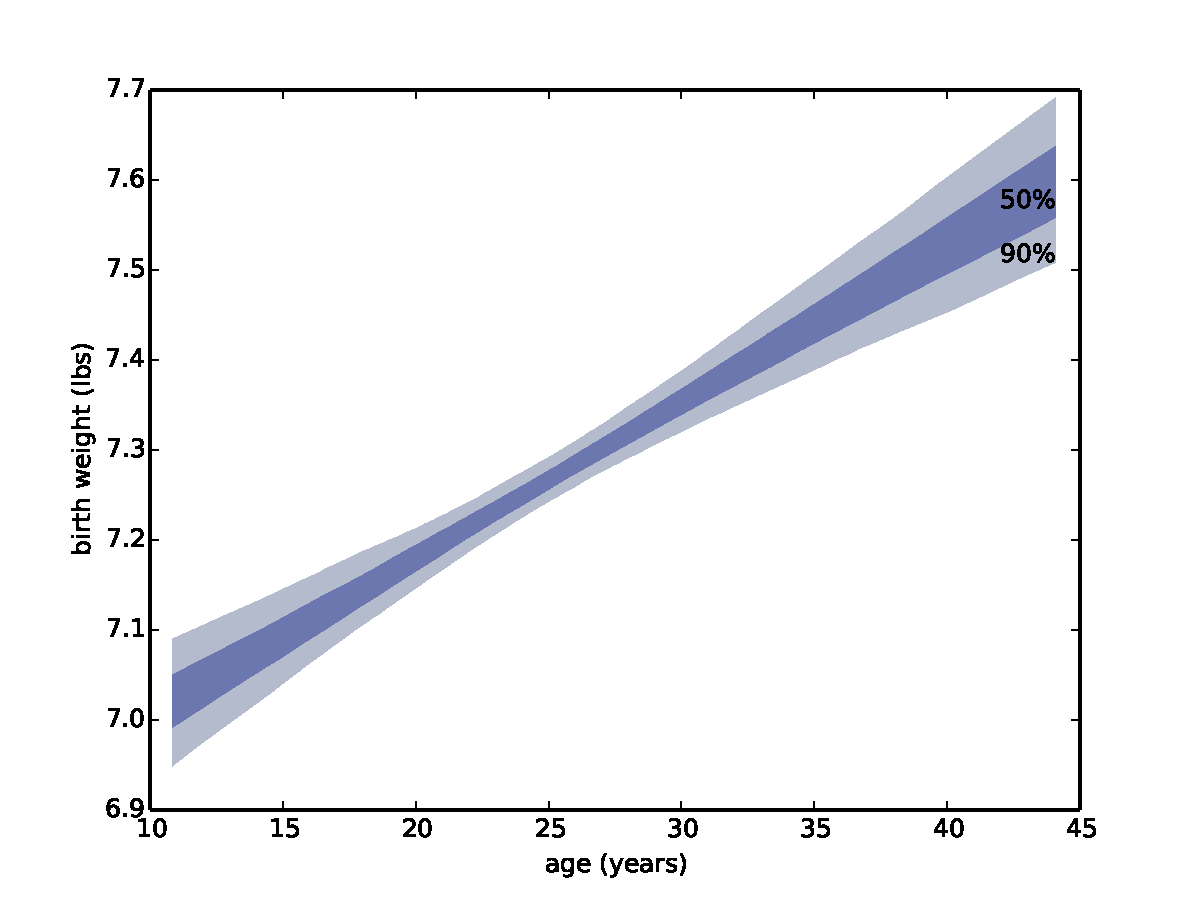
\includegraphics[height=2.5in]{figs/linear3.pdf}}
\caption{50\% and 90\% confidence intervals showing variability in the
  fitted line due to sampling error of {\tt inter} and {\tt slope}.}
\label{linear3}
\end{figure}

Figure~\ref{linear3} shows the 50\% and 90\% confidence
intervals for curves fitted to birth weight as a function of
mother's age.
  The vertical width of the region represents the effect of
sampling error; the effect is smaller for values near the mean and
larger for the extremes.


\section{Goodness of fit}
\label{goodness}
\index{goodness of fit}

There are several ways to measure the quality of a linear model, or
{\bf goodness of fit}.  One of the simplest is the standard deviation
of the residuals.
\index{standard deviation}
\index{model}

If you use a linear model to make predictions, {\tt Std(res)}
is the root mean squared error (RMSE) of your predictions.  For
example, if you use mother's age to guess birth weight, the RMSE of
your guess would be 1.40 lbs.
\index{birth weight}
\index{weight!birth}

If you guess birth weight without knowing the mother's age, the RMSE
of your guess is {\tt Std(ys)}, which is 1.41 lbs.  So in this
example, knowing a mother's age does not improve the predictions
substantially.
\index{prediction}

Another way to measure goodness of fit is  the {\bf
  coefficient of determination}, usually denoted $R^2$ and 
called ``R-squared'':
\index{coefficient of determination}
\index{r-squared}

\begin{verbatim}
def CoefDetermination(ys, res):
    return 1 - Var(res) / Var(ys)
\end{verbatim}

{\tt Var(res)} is the MSE of your guesses using the model,
{\tt Var(ys)} is the MSE without it.   So their ratio is the fraction
of MSE that remains if you use the model, and $R^2$ is the fraction
of MSE the model eliminates.
\index{MSE}

For birth weight and mother's age, $R^2$ is 0.0047, which means
that mother's age predicts about half of 1\% of variance in
birth weight.

There is a simple relationship between the coefficient of
determination and Pearson's coefficient of correlation: $R^2 = \rho^2$.
For example, if $\rho$ is 0.8 or -0.8, $R^2 = 0.64$.
\index{Pearson coefficient of correlation}

Although $\rho$ and $R^2$ are often used to quantify the strength of a
relationship, they are not easy to interpret in terms of predictive
power.  In my opinion, {\tt Std(res)} is the best representation
of the quality of prediction, especially if it is presented
in relation to {\tt Std(ys)}.
\index{coefficient of determination}
\index{r-squared}

For example, when people talk about the validity of the SAT
(a standardized test used for college admission in the U.S.) they
often talk about correlations between SAT scores and other measures of
intelligence.
\index{SAT}
\index{IQ}

According to one study, there is a Pearson correlation of
$\rho=0.72$ between total SAT scores and IQ scores, which sounds like
a strong correlation.  But $R^2 = \rho^2 = 0.52$, so SAT scores
account for only 52\% of variance in IQ.

IQ scores are normalized with {\tt Std(ys) = 15}, so

\begin{verbatim}
>>> var_ys = 15**2
>>> rho = 0.72
>>> r2 = rho**2
>>> var_res = (1 - r2) * var_ys
>>> std_res = math.sqrt(var_res)
10.4096
\end{verbatim}

So using SAT score to predict IQ reduces RMSE from 15 points to 10.4
points.  A correlation of 0.72 yields a reduction in RMSE of only
31\%.

If you see a correlation that looks impressive, remember that $R^2$ is
a better indicator of reduction in MSE, and reduction in RMSE is a
better indicator of predictive power.
\index{coefficient of determination}
\index{r-squared}
\index{prediction}


\section{Testing a linear model}

The effect of mother's age on birth weight is small, and has little
predictive power.  So is it possible that the apparent relationship
is due to chance?  There are several ways we might test the
results of a linear fit.
\index{birth weight}
\index{weight!birth}
\index{model}
\index{linear model}

One option is to test whether the apparent reduction in MSE is due to
chance.  In that case, the test statistic is $R^2$ and the null
hypothesis is that there is no relationship between the variables.  We
can simulate the null hypothesis by permutation, as in
Section~\ref{corrtest}, when we tested the correlation between
mother's age and birth weight.  In fact, because $R^2 = \rho^2$, a
one-sided test of $R^2$ is equivalent to a two-sided test of $\rho$.
We've already done that test, and found $p < 0.001$, so we conclude
that the apparent relationship between mother's age and birth weight
is statistically significant.
\index{null hypothesis}
\index{permutation}
\index{coefficient of determination}
\index{r-squared}
  \index{significant} \index{statistically significant}

Another approach is to test whether the apparent slope is due to chance.
The null hypothesis is that the slope is actually zero; in that case
we can model the birth weights as random variations around their mean.
Here's a HypothesisTest for this model:
\index{HypothesisTest}
\index{model}

\begin{verbatim}
class SlopeTest(thinkstats2.HypothesisTest):

    def TestStatistic(self, data):
        ages, weights = data
        _, slope = thinkstats2.LeastSquares(ages, weights)
        return slope

    def MakeModel(self):
        _, weights = self.data
        self.ybar = weights.mean()
        self.res = weights - self.ybar

    def RunModel(self):
        ages, _ = self.data
        weights = self.ybar + np.random.permutation(self.res)
        return ages, weights
\end{verbatim}

The data are represented as sequences of ages and weights.  The
test statistic is the slope estimated by {\tt LeastSquares}.
The model of the null hypothesis is represented by the mean weight
of all babies and the deviations from the mean.  To
generate simulated data, we permute the deviations and add them to
the mean.
\index{deviation}
\index{null hypothesis}
\index{permutation}

Here's the code that runs the hypothesis test:

\begin{verbatim}
    live, firsts, others = first.MakeFrames()
    live = live.dropna(subset=['agepreg', 'totalwgt_lb'])
    ht = SlopeTest((live.agepreg, live.totalwgt_lb))
    pvalue = ht.PValue()
\end{verbatim}

The p-value is less than $0.001$, so although the estimated
slope is small, it is unlikely to be due to chance.
\index{p-value}
\index{dropna}
\index{NaN}

Estimating the p-value by simulating the null hypothesis is strictly
correct, but there is a simpler alternative.  Remember that we already
computed the sampling distribution of the slope, in
Section~\ref{regest}.  To do that, we assumed that the observed slope
was correct and simulated experiments by resampling.
\index{null hypothesis}

Figure~\ref{linear4} shows the sampling distribution of the
slope, from Section~\ref{regest}, and the distribution of slopes
generated under the null hypothesis.  The sampling distribution
is centered about the estimated slope, 0.017 lbs/year, and the slopes
under the null hypothesis are centered around 0; but other than
that, the distributions are identical.  The distributions are
also symmetric, for reasons we will see in Section~\ref{CLT}.
\index{symmetric}
\index{sampling distribution}

\begin{figure}
% linear.py
\centerline{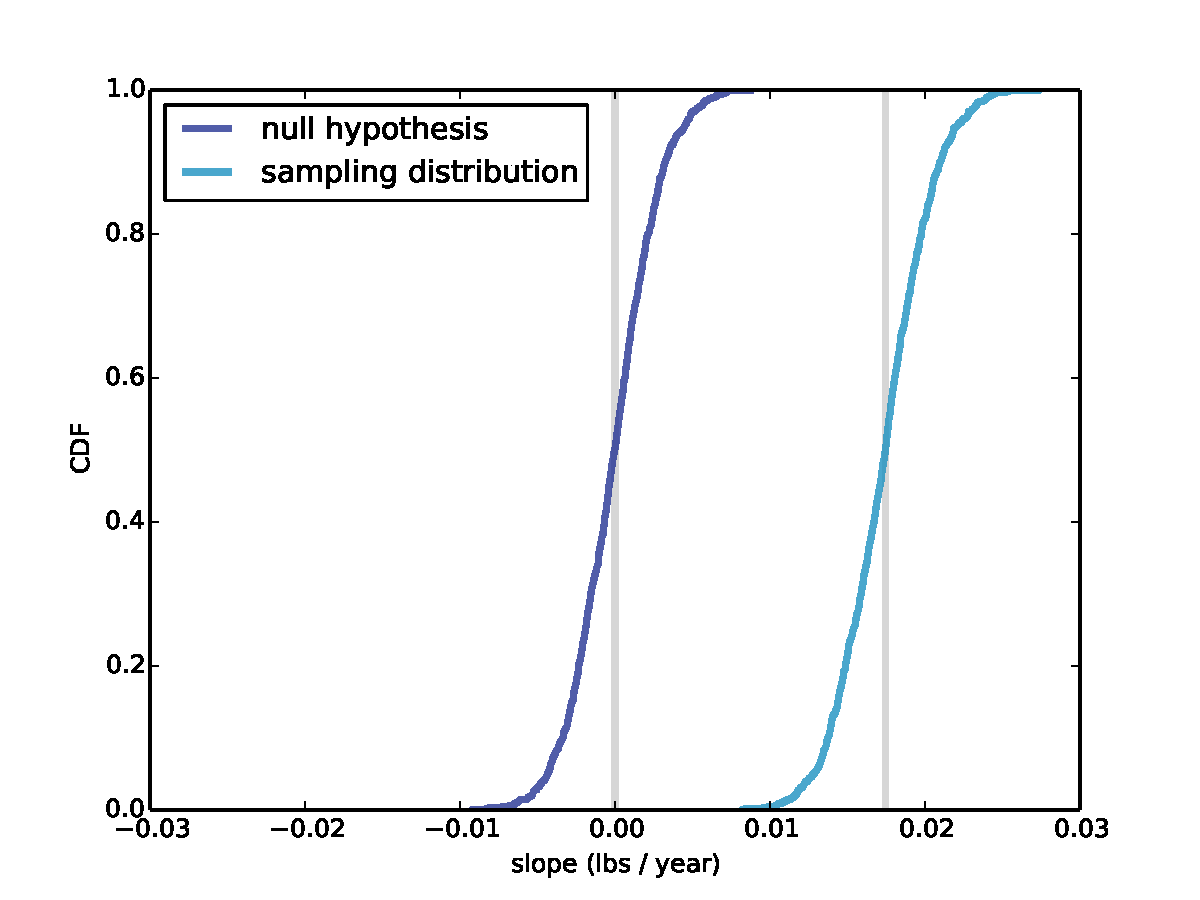
\includegraphics[height=2.5in]{figs/linear4.pdf}}
\caption{The sampling distribution of the estimated
slope and the distribution of slopes
generated under the null hypothesis.  The vertical lines are at 0
and the observed slope, 0.017 lbs/year.}
\label{linear4}
\end{figure}

So we could estimate the p-value two ways:
\index{p-value}

\begin{itemize}

\item Compute the probability that the slope under the null
hypothesis exceeds the observed slope.
\index{null hypothesis}

\item Compute the probability that the slope in the sampling
distribution falls below 0.  (If the estimated slope were negative,
we would compute the probability that the slope in the sampling
distribution exceeds 0.)

\end{itemize}

The second option is easier because we normally want to compute the
sampling distribution of the parameters anyway.  And it is a good
approximation unless the sample size is small {\em and} the
distribution of residuals is skewed.  Even then, it is usually good
enough, because p-values don't have to be precise.
\index{skewness}
\index{parameter}

Here's the code that estimates the p-value of the slope using the
sampling distribution:
\index{sampling distribution}

\begin{verbatim}
    inters, slopes = SamplingDistributions(live, iters=1001)
    slope_cdf = thinkstats2.Cdf(slopes)
    pvalue = slope_cdf[0]
\end{verbatim}

Again, we find $p < 0.001$.  


\section{Weighted resampling}
\label{weighted}

So far we have treated the NSFG data as if it were a representative
sample, but as I mentioned in Section~\ref{nsfg}, it is not.  The
survey deliberately oversamples several groups in order to
improve the chance of getting statistically significant results; that
is, in order to improve the power of tests involving these groups.
  \index{significant} \index{statistically significant}

This survey design is useful for many purposes, but it means that we
cannot use the sample to estimate values for the general
population without accounting for the sampling process.

For each respondent, the NSFG data includes a variable called {\tt
  finalwgt}, which is the number of people in the general population
the respondent represents.  This value is called a {\bf sampling
  weight}, or just ``weight.''
\index{sampling weight}
\index{weight}
\index{weighted resampling}
\index{resampling!weighted}

As an example, if you survey 100,000 people in a country of 300
million, each respondent represents 3,000 people.  If you oversample
one group by a factor of 2, each person in the oversampled
group would have a lower weight, about 1500.

To correct for oversampling, we can use resampling; that is, we
can draw samples from the survey using probabilities proportional
to sampling weights.  Then, for any quantity we want to estimate, we can
generate sampling distributions, standard errors, and confidence
intervals.  As an example, I will estimate mean birth weight with
and without sampling weights.
\index{standard error}
\index{confidence interval}
\index{birth weight}
\index{weight!birth}
\index{sampling distribution}
\index{oversampling}

In Section~\ref{regest}, we saw {\tt ResampleRows}, which chooses
rows from a DataFrame, giving each row the same probability.
Now we need to do the same thing using probabilities
proportional to sampling weights.
{\tt ResampleRowsWeighted} takes a DataFrame, resamples rows according
to the weights in {\tt finalwgt}, and returns a DataFrame containing
the resampled rows:
\index{DataFrame}
\index{resampling}

\begin{verbatim}
def ResampleRowsWeighted(df, column='finalwgt'):
    weights = df[column]
    cdf = Cdf(dict(weights))
    indices = cdf.Sample(len(weights))
    sample = df.loc[indices]
    return sample
\end{verbatim}

{\tt weights} is a Series; converting it to a dictionary makes
a map from the indices to the weights.  In {\tt cdf} the values
are indices and the probabilities are proportional to the
weights.

{\tt indices} is a sequence of row indices; {\tt sample} is a
DataFrame that contains the selected rows.  Since we sample with
replacement, the same row might appear more than once.  \index{Cdf}
\index{replacement}

Now we can compare the effect of resampling with and without
weights.  Without weights, we generate the sampling distribution
like this:
\index{sampling distribution}

\begin{verbatim}
    estimates = [ResampleRows(live).totalwgt_lb.mean()
                 for _ in range(iters)]
\end{verbatim}

With weights, it looks like this:

\begin{verbatim}
    estimates = [ResampleRowsWeighted(live).totalwgt_lb.mean()
                 for _ in range(iters)]
\end{verbatim}

The following table summarizes the results:

\begin{center}
\begin{tabular}{|l|c|c|c|}
\hline
                    &  mean birth   & standard  &  90\% CI  \\ 
                    &  weight (lbs) & error     &           \\ 
\hline
Unweighted          &  7.27  &  0.014  &  (7.24, 7.29)  \\ 
Weighted            &  7.35  &  0.014  &  (7.32, 7.37)  \\ 
\hline
\end{tabular}
\end{center}

%mean 7.26580789518
%stderr 0.0141683527792
%ci (7.2428565501217079, 7.2890814917127074)
%mean 7.34778034718
%stderr 0.0142738972319
%ci (7.3232804012858885, 7.3704916897506925)

In this example, the effect of weighting is small but non-negligible.
The difference in estimated means, with and without weighting, is
about 0.08 pounds, or 1.3 ounces.  This difference is substantially
larger than the standard error of the estimate, 0.014 pounds, which
implies that the difference is not due to chance.
\index{standard error}
\index{confidence interval}


\section{Exercises}

A solution to this exercise is in \verb"chap10soln.ipynb"

\begin{exercise}

Using the data from the BRFSS, compute the linear least squares
fit for log(weight) versus height.
How would you best present the estimated parameters for a model
like this where one of the variables is log-transformed?
If you were trying to guess
someone's weight, how much would it help to know their height?
\index{Behavioral Risk Factor Surveillance System}
\index{BRFSS}
\index{model}

Like the NSFG, the BRFSS oversamples some groups and provides
a sampling weight for each respondent.  In the BRFSS data, the variable
name for these weights is {\tt totalwt}.
Use resampling, with and without weights, to estimate the mean height
of respondents in the BRFSS, the standard error of the mean, and a
90\% confidence interval.  How much does correct weighting affect the
estimates?
\index{confidence interval}
\index{standard error}
\index{oversampling}
\index{sampling weight}
\end{exercise}


\section{Glossary}

\begin{itemize}

\item linear fit: a line intended to model the relationship between
variables.  \index{linear fit}

\item least squares fit: A model of a dataset that minimizes the
sum of squares of the residuals.
\index{least squares fit}

\item residual: The deviation of an actual value from a model.
\index{residuals}

\item goodness of fit: A measure of how well a model fits data.
\index{goodness of fit}

\item coefficient of determination: A statistic intended to
quantify goodness of fit.
\index{coefficient of determination}

\item sampling weight: A value associated with an observation in a
  sample that indicates what part of the population it represents.
\index{sampling weight}

\end{itemize}



\chapter{Regression}
\label{regression}

The linear least squares fit in the previous chapter is an example of
{\bf regression}, which is the more general problem of fitting any
kind of model to any kind of data.  This use of the term ``regression''
is a historical accident; it is only indirectly related to the
original meaning of the word.
\index{model}
\index{regression}

The goal of regression analysis is to describe the relationship
between one set of variables, called the {\bf dependent variables},
and another set of variables, called independent or {\bf
  explanatory variables}.
\index{explanatory variable}
\index{dependent variable}

In the previous chapter we used mother's age as an explanatory
variable to predict birth weight as a dependent variable.  When there
is only one dependent and one explanatory variable, that's {\bf
  simple regression}.  In this chapter, we move on to {\bf multiple
  regression}, with more than one explanatory variable.  If there is
more than one dependent variable, that's multivariate
regression.
\index{birth weight}
\index{weight!birth}
\index{simple regression}
\index{multiple regression}

If the relationship between the dependent and explanatory variable
is linear, that's {\bf linear regression}.  For example,
if the dependent variable is $y$ and the explanatory variables
are $x_1$ and $x_2$, we would write the following linear
regression model:
%
\[ y = \beta_0 + \beta_1 x_1 + \beta_2 x_2 + \eps \]
%
where $\beta_0$ is the intercept, $\beta_1$ is the parameter
associated with $x_1$, $\beta_2$ is the parameter associated with
$x_2$, and $\eps$ is the residual due to random variation or other
unknown factors.
\index{regression model}
\index{linear regression}

Given a sequence of values for $y$ and sequences for $x_1$ and $x_2$,
we can find the parameters, $\beta_0$, $\beta_1$, and $\beta_2$, that
minimize the sum of $\eps^2$.  This process is called
{\bf ordinary least squares}.  The computation is similar to {\tt
  thinkstats2.LeastSquare}, but generalized to deal with more than one
explanatory variable.  You can find the details at
\url{https://en.wikipedia.org/wiki/Ordinary_least_squares}
\index{explanatory variable}
\index{ordinary least squares}
\index{parameter}

The code for this chapter is in {\tt regression.py}.  For information
about downloading and working with this code, see Section~\ref{code}.

\section{StatsModels}
\label{statsmodels}

In the previous chapter I presented {\tt thinkstats2.LeastSquares}, an
implementation of simple linear regression intended to be easy to
read.  For multiple regression we'll switch to StatsModels, a Python
package that provides several forms of regression and other
analyses.  If you are using Anaconda, you already have StatsModels;
otherwise you might have to install it.
\index{Anaconda}

As an example, I'll run the model from the previous chapter with
StatsModels:
\index{StatsModels}
\index{model}

\begin{verbatim}
    import statsmodels.formula.api as smf

    live, firsts, others = first.MakeFrames()
    formula = 'totalwgt_lb ~ agepreg'
    model = smf.ols(formula, data=live)
    results = model.fit()
\end{verbatim}

{\tt statsmodels} provides two interfaces (APIs); the ``formula''
API uses strings to identify the dependent and explanatory variables.
It uses a syntax called {\tt patsy}; in this example, the \verb"~"
operator separates the dependent variable on the left from the
explanatory variables on the right.
\index{explanatory variable}
\index{dependent variable}
\index{Patsy}

{\tt smf.ols} takes the formula string and the DataFrame, {\tt live},
and returns an OLS object that represents the model.  The name {\tt ols}
stands for ``ordinary least squares.''
\index{DataFrame}
\index{model}
\index{ordinary least squares}

The {\tt fit} method fits the model to the data and returns a
RegressionResults object that contains the results.
\index{RegressionResults}

The results are also available as attributes.  {\tt params}
is a Series that maps from variable names to their parameters, so we can
get the intercept and slope like this:
\index{Series}

\begin{verbatim}
    inter = results.params['Intercept']
    slope = results.params['agepreg']
\end{verbatim}

The estimated parameters are 6.83 and 0.0175, the same as
from {\tt LeastSquares}.
\index{parameter}

{\tt pvalues} is a Series that maps from variable names to the associated
p-values, so we can check whether the estimated slope is statistically
significant:
\index{p-value}
  \index{significant} \index{statistically significant}

\begin{verbatim}
    slope_pvalue = results.pvalues['agepreg']
\end{verbatim}

The p-value associated with {\tt agepreg} is {\tt 5.7e-11}, which
is less than $0.001$, as expected.
\index{age}

{\tt results.rsquared} contains $R^2$, which is $0.0047$.  {\tt
  results} also provides \verb"f_pvalue", which is the p-value
associated with the model as a whole, similar to testing whether $R^2$
is statistically significant.
\index{model}
\index{coefficient of determination}
\index{r-squared}

And {\tt results} provides {\tt resid}, a sequence of residuals, and
{\tt fittedvalues}, a sequence of fitted values corresponding to
{\tt agepreg}.
\index{residuals}

The results object provides {\tt summary()}, which
represents the results in a readable format.  

\begin{verbatim}
    print(results.summary())
\end{verbatim}

But it prints a lot of information that is not relevant (yet), so
I use a simpler function called {\tt SummarizeResults}.  Here are
the results of this model:

\begin{verbatim}
Intercept       6.83    (0)
agepreg         0.0175  (5.72e-11)
R^2 0.004738
Std(ys) 1.408
Std(res) 1.405
\end{verbatim}

{\tt Std(ys)} is the standard deviation of the dependent variable,
which is the RMSE if you have to guess birth weights without the benefit of
any explanatory variables.  {\tt Std(res)} is the standard deviation
of the residuals, which is the RMSE if your guesses are informed
by the mother's age.  As we have already seen, knowing the mother's
age provides no substantial improvement to the predictions.
\index{standard deviation}
\index{birth weight}
\index{weight!birth}
\index{explanatory variable}
\index{dependent variable}
\index{RMSE}
\index{predictive power}


\section{Multiple regression}
\label{multiple}

In Section~\ref{birth_weights} we saw that first babies tend to be
lighter than others, and this effect is statistically significant.
But it is a strange result because there is no obvious mechanism that
would cause first babies to be lighter.  So we might wonder whether
this relationship is {\bf spurious}.
\index{multiple regression}
\index{spurious relationship}

In fact, there is a possible explanation for this effect.  We have
seen that birth weight depends on mother's age, and we might expect
that mothers of first babies are younger than others.
\index{weight}
\index{age}

With a few calculations we can check whether this explanation
is plausible.  Then we'll use multiple regression to investigate
more carefully.  First, let's see how big the difference in weight
is:

\begin{verbatim}
diff_weight = firsts.totalwgt_lb.mean() - others.totalwgt_lb.mean()
\end{verbatim}

First babies are 0.125 lbs lighter, or 2 ounces.  And the difference
in ages:

\begin{verbatim}
diff_age = firsts.agepreg.mean() - others.agepreg.mean()
\end{verbatim}

The mothers of first babies are 3.59 years younger.  Running the
linear model again, we get the change in birth weight as a function
of age:
\index{birth weight}
\index{weight!birth}

\begin{verbatim}
results = smf.ols('totalwgt_lb ~ agepreg', data=live).fit()
slope = results.params['agepreg']
\end{verbatim}

The slope is 0.0175 pounds per year.  If we multiply the slope by
the difference in ages, we get the expected difference in birth
weight for first babies and others, due to mother's age:

\begin{verbatim}
slope * diff_age
\end{verbatim}

The result is 0.063, just about half of the observed difference.
So we conclude, tentatively, that the observed difference in birth
weight can be partly explained by the difference in mother's age. 

Using multiple regression, we can explore these relationships
more systematically.
\index{multiple regression}

\begin{verbatim}
    live['isfirst'] = live.birthord == 1
    formula = 'totalwgt_lb ~ isfirst'
    results = smf.ols(formula, data=live).fit()
\end{verbatim}

The first line creates a new column named {\tt isfirst} that is
True for first babies and false otherwise.  Then we fit a model
using {\tt isfirst} as an explanatory variable.
\index{model}
\index{explanatory variable}

Here are the results:

\begin{verbatim}
Intercept         7.33   (0)
isfirst[T.True]  -0.125  (2.55e-05)
R^2 0.00196
\end{verbatim}

Because {\tt isfirst} is a boolean, {\tt ols} treats it as a
{\bf categorical variable}, which means that the values fall
into categories, like True and False, and should not be treated
as numbers.  The estimated parameter is the effect on birth
weight when {\tt isfirst} is true, so the result,
-0.125 lbs, is the difference in
birth weight between first babies and others.  
\index{birth weight}
\index{weight!birth}
\index{categorical variable}
\index{boolean}

The slope and the intercept are statistically significant,
which means that they were unlikely to occur by chance, but the
the $R^2$ value for this model is small, which means that
{\tt isfirst} doesn't account for a substantial part of the
variation in birth weight.
\index{coefficient of determination}
\index{r-squared}

The results are similar with {\tt agepreg}:

\begin{verbatim}
Intercept       6.83    (0)
agepreg         0.0175  (5.72e-11)
R^2 0.004738
\end{verbatim}

Again, the parameters are statistically significant, but
$R^2$ is low.
\index{coefficient of determination}
\index{r-squared}

These models confirm results we have already seen.  But now we
can fit a single model that includes both variables.  With the
formula \verb"totalwgt_lb ~ isfirst + agepreg", we get:

\begin{verbatim}
Intercept        6.91    (0)
isfirst[T.True] -0.0698  (0.0253)
agepreg          0.0154  (3.93e-08)
R^2 0.005289
\end{verbatim}

In the combined model, the parameter for {\tt isfirst} is smaller
by about half, which means that part of the apparent effect of
{\tt isfirst} is actually accounted for by {\tt agepreg}.  And
the p-value for {\tt isfirst} is about 2.5\%, which is on the
border of statistical significance.
\index{p-value}
\index{model}

$R^2$ for this model is a little higher, which indicates that the
two variables together account for more variation in birth weight
than either alone (but not by much).
\index{birth weight}
\index{weight!birth}
\index{coefficient of determination}
\index{r-squared}


\section{Nonlinear relationships}
\label{nonlinear}

Remembering that the contribution of {\tt agepreg} might be nonlinear,
we might consider adding a variable to capture more of this
relationship.  One option is to create a column, {\tt agepreg2},
that contains the squares of the ages:
\index{nonlinear}

\begin{verbatim}
    live['agepreg2'] = live.agepreg**2
    formula = 'totalwgt_lb ~ isfirst + agepreg + agepreg2'
\end{verbatim}

Now by estimating parameters for {\tt agepreg} and {\tt agepreg2},
we are effectively fitting a parabola:

\begin{verbatim}
Intercept        5.69     (1.38e-86)
isfirst[T.True] -0.0504   (0.109)
agepreg          0.112    (3.23e-07)
agepreg2        -0.00185  (8.8e-06)
R^2 0.007462
\end{verbatim}

The parameter of {\tt agepreg2} is negative, so the parabola
curves downward, which is consistent with the shape of the lines
in Figure~\ref{linear2}.
\index{parabola}

The quadratic model of {\tt agepreg} accounts for more of the
variability in birth weight; the parameter for {\tt isfirst}
is smaller in this model, and no longer statistically significant.
\index{birth weight}
\index{weight!birth}
\index{quadratic model}
\index{model}
  \index{significant} \index{statistically significant}

Using computed variables like {\tt agepreg2} is a common way to
fit polynomials and other functions to data.  
This process is still considered linear
regression, because the dependent variable is a linear function of
the explanatory variables, regardless of whether some variables
are nonlinear functions of others.
\index{explanatory variable}
\index{dependent variable}
\index{nonlinear}

The following table summarizes the results of these regressions:

\begin{center}
\begin{tabular}{|l|c|c|c|c|}
\hline & isfirst & agepreg & agepreg2 & $R^2$ \\ \hline
Model 1 & -0.125 * & -- & -- & 0.002 \\
Model 2 & -- & 0.0175 * & -- & 0.0047 \\
Model 3 & -0.0698 (0.025) & 0.0154 * & -- & 0.0053 \\
Model 4 & -0.0504 (0.11) & 0.112 * & -0.00185 * & 0.0075 \\
\hline
\end{tabular}
\end{center}

The columns in this table are the explanatory variables and
the coefficient of determination, $R^2$.  Each entry is an estimated
parameter and either a p-value in parentheses or an asterisk to
indicate a p-value less that 0.001.
\index{p-value}
\index{coefficient of determination}
\index{r-squared}
\index{explanatory variable}

We conclude that the apparent difference in birth weight
is explained, at least in part, by the difference in mother's age.
When we include mother's age in the model, the effect of
{\tt isfirst} gets smaller, and the remaining effect might be
due to chance.
\index{age}

In this example, mother's age acts as a {\bf control variable};
including {\tt agepreg} in the model ``controls for'' the
difference in age between first-time mothers and others, making
it possible to isolate the effect (if any) of {\tt isfirst}. 
\index{control variable}


\section{Data mining}
\label{mining}

So far we have used regression models for explanation; for example,
in the previous section we discovered that an apparent difference
in birth weight is actually due to a difference in mother's age.
But the $R^2$ values of those models is very low, which means that
they have little predictive power.  In this section we'll try to
do better.
\index{birth weight}
\index{weight!birth}
\index{regression model}
\index{coefficient of determination}
\index{r-squared}

Suppose one of your co-workers is expecting a baby and
there is an office pool to guess the baby's birth weight (if you are
not familiar with betting pools, see
\url{https://en.wikipedia.org/wiki/Betting_pool}).
\index{betting pool}

Now suppose that you {\em really} want to win the pool.  What could
you do to improve your chances?  Well, 
the NSFG dataset includes 244 variables about each pregnancy and another
3087 variables about each respondent.  Maybe some of those variables
have predictive power.  To find out which ones are most useful,
why not try them all?
\index{NSFG}

Testing the variables in the pregnancy table is easy, but in order to
use the variables in the respondent table, we have to match up each
pregnancy with a respondent.  In theory we could iterate through the
rows of the pregnancy table, use the {\tt caseid} to find the
corresponding respondent, and copy the values from the
correspondent table into the pregnancy table.  But that would be slow.
\index{join}
\index{SQL}

A better option is to recognize this process as a {\bf join} operation
as defined in SQL and other relational database languages (see
\url{https://en.wikipedia.org/wiki/Join_(SQL)}).  Join is implemented
as a DataFrame method, so we can perform the operation like this:
\index{DataFrame}

\begin{verbatim}
    live = live[live.prglngth>30]
    resp = chap01soln.ReadFemResp()
    resp.index = resp.caseid
    join = live.join(resp, on='caseid', rsuffix='_r')
\end{verbatim}

The first line selects records for pregnancies longer than 30 weeks,
assuming that the office pool is formed several weeks before the
due date.
\index{betting pool}

The next line reads the respondent file.  The result is a DataFrame
with integer indices; in order to look up respondents efficiently,
I replace {\tt resp.index} with {\tt resp.caseid}. 

The {\tt join} method is invoked on {\tt live}, which is considered
the ``left'' table, and passed {\tt resp}, which is the ``right'' table.
The keyword argument {\tt on} indicates the variable used to match up
rows from the two tables.

In this example some column names appear in both tables,
so we have to provide {\tt rsuffix}, which is a string that will be
appended to the names of overlapping columns from the right table.
For example, both tables have a column named {\tt race} that encodes
the race of the respondent.  The result of the join contains two
columns named {\tt race} and \verb"race_r".
\index{race}

The pandas implementation is fast.  Joining the NSFG tables takes
less than a second on an ordinary desktop computer.
Now we can start testing variables.
\index{pandas}
\index{join}

\begin{verbatim}
    t = []
    for name in join.columns:
        try:
            if join[name].var() < 1e-7:
                continue

            formula = 'totalwgt_lb ~ agepreg + ' + name
            model = smf.ols(formula, data=join)
            if model.nobs < len(join)/2:
                continue

            results = model.fit()
        except (ValueError, TypeError):
            continue

        t.append((results.rsquared, name))
\end{verbatim}

For each variable we construct a model, compute $R^2$, and append
the results to a list.  The models all include {\tt agepreg}, since
we already know that it has some predictive power.
\index{model}
\index{coefficient of determination}
\index{r-squared}

I check that each explanatory variable has some variability; otherwise
the results of the regression are unreliable.  I also check the number
of observations for each model.  Variables that contain a large number
of {\tt nan}s are not good candidates for prediction.
\index{explanatory variable}
\index{NaN}

For most of these variables, we haven't done any cleaning.  Some of them
are encoded in ways that don't work very well for linear regression.
As a result, we might overlook some variables that would be useful if
they were cleaned properly.  But maybe we will find some good candidates.
\index{cleaning}


\section{Prediction}

The next step is to sort the results and select the variables that
yield the highest values of $R^2$.
\index{prediction}

\begin{verbatim}
    t.sort(reverse=True)
    for mse, name in t[:30]:
        print(name, mse)
\end{verbatim}

The first variable on the list is \verb"totalwgt_lb",
followed by \verb"birthwgt_lb".  Obviously, we can't use birth
weight to predict birth weight.
\index{birth weight}
\index{weight!birth}

Similarly {\tt prglngth} has useful predictive power, but for the
office pool we assume pregnancy length (and the related variables)
are not known yet.
\index{predictive power}
\index{pregnancy length}

The first useful predictive variable is {\tt babysex} which indicates
whether the baby is male or female.  In the NSFG dataset, boys are
about 0.3 lbs heavier.  So, assuming that the sex of the baby is
known, we can use it for prediction.
\index{sex}

Next is {\tt race}, which indicates whether the respondent is white,
black, or other.  As an explanatory variable, race can be problematic.
In datasets like the NSFG, race is correlated with many other
variables, including income and other socioeconomic factors.  In a
regression model, race acts as a {\bf proxy variable},
so apparent correlations with race are often caused, at least in
part, by other factors.
\index{explanatory variable}
\index{race}

The next variable on the list is {\tt nbrnaliv}, which indicates
whether the pregnancy yielded multiple births.  Twins and triplets
tend to be smaller than other babies, so if we know whether our
hypothetical co-worker is expecting twins, that would help.
\index{multiple birth}

Next on the list is {\tt paydu}, which indicates whether the
respondent owns her home.  It is one of several income-related
variables that turn out to be predictive.  In datasets like the NSFG,
income and wealth are correlated with just about everything.  In this
example, income is related to diet, health, health care, and other
factors likely to affect birth weight.
\index{birth weight}
\index{weight!birth}
\index{income}
\index{wealth}

Some of the other variables on the list are things that would not
be known until later, like {\tt bfeedwks}, the number of weeks
the baby was breast fed.  We can't use these variables for prediction,
but you might want to speculate on reasons
{\tt bfeedwks} might be correlated with birth weight.

Sometimes you start with a theory and use data to test it.  Other
times you start with data and go looking for possible theories.
The second approach, which this section demonstrates, is
called {\bf data mining}.  An advantage of data mining is that it
can discover unexpected patterns.  A hazard is that many of the
patterns it discovers are either random or spurious.
\index{theory}
\index{data mining}

Having identified potential explanatory variables, I tested a few
models and settled on this one:
\index{model}
\index{explanatory variable}

\begin{verbatim}
    formula = ('totalwgt_lb ~ agepreg + C(race) + babysex==1 + '
               'nbrnaliv>1 + paydu==1 + totincr')
    results = smf.ols(formula, data=join).fit()
\end{verbatim}

This formula uses some syntax we have not seen yet:
{\tt C(race)} tells the formula parser (Patsy) to treat race as a
categorical variable, even though it is encoded numerically.
\index{Patsy}
\index{categorical variable}

The encoding for {\tt babysex} is 1 for male, 2 for female; writing
{\tt babysex==1} converts it to boolean, True for male and false for
female.
\index{boolean}

Similarly {\tt nbrnaliv>1} is True for multiple births and 
{\tt paydu==1} is True for respondents who own their houses.

{\tt totincr} is encoded numerically from 1-14, with each increment
representing about \$5000 in annual income.  So we can treat these
values as numerical, expressed in units of \$5000.
\index{income}

Here are the results of the model:

\begin{verbatim}
Intercept               6.63    (0)
C(race)[T.2]            0.357   (5.43e-29)
C(race)[T.3]            0.266   (2.33e-07)
babysex == 1[T.True]    0.295   (5.39e-29)
nbrnaliv > 1[T.True]   -1.38    (5.1e-37)
paydu == 1[T.True]      0.12    (0.000114)
agepreg                 0.00741 (0.0035)
totincr                 0.0122  (0.00188)
\end{verbatim}

The estimated parameters for race are larger than I expected,
especially since we control for income.  The encoding
is 1 for black, 2 for white, and 3 for other.  Babies of black
mothers are lighter than babies of other races by 0.27--0.36 lbs.
\index{control variable}
\index{race}

As we've already seen, boys are heavier by about 0.3 lbs;
twins and other multiplets are lighter by 1.4 lbs.
\index{weight}

People who own their homes have heavier babies by about 0.12 lbs,
even when we control for income.  The parameter for mother's
age is smaller than what we saw in Section~\ref{multiple}, which
suggests that some of the other variables are correlated with
age, probably including {\tt paydu} and {\tt totincr}.
\index{income}

All of these variables are statistically significant, some with
very low p-values, but 
$R^2$ is only 0.06, still quite small.
RMSE without using the model is 1.27 lbs; with the model it drops
to 1.23.  So your chance of winning the pool is not substantially
improved.  Sorry!
\index{p-value}
\index{model}
\index{coefficient of determination}
\index{r-squared}
  \index{significant} \index{statistically significant}



\section{Logistic regression}

In the previous examples, some of the explanatory variables were
numerical and some categorical (including boolean).  But the dependent
variable was always numerical.
\index{explanatory variable}
\index{dependent variable}
\index{categorical variable}

Linear regression can be generalized to handle other kinds of
dependent variables.  If the dependent variable is boolean, the
generalized model is called {\bf logistic regression}.  If the dependent
variable is an integer count, it's called {\bf Poisson
regression}.
\index{model}
\index{logistic regression}
\index{Poisson regression}
\index{boolean}

As an example of logistic regression, let's consider a variation
on the office pool scenario.
Suppose
a friend of yours is pregnant and you want to predict whether the
baby is a boy or a girl.  You could use data from the NSFG to find
factors that affect the ``sex ratio'', which is conventionally
defined to be the probability
of having a boy.
\index{betting pool}
\index{sex}

If you encode the dependent variable numerically, for example 0 for a
girl and 1 for a boy, you could apply ordinary least squares, but
there would be problems.  The linear model might be something like
this:
%
\[ y = \beta_0 + \beta_1 x_1 + \beta_2 x_2 + \eps \]
%
Where $y$ is the dependent variable, and $x_1$ and $x_2$ are
explanatory variables.  Then we could find the parameters that
minimize the residuals.
\index{regression model}
\index{explanatory variable}
\index{dependent variable}
\index{ordinary least squares}

The problem with this approach is that it produces predictions that
are hard to interpret.  Given estimated parameters and values for
$x_1$ and $x_2$, the model might predict $y=0.5$, but the only
meaningful values of $y$ are 0 and 1.
\index{parameter}

It is tempting to interpret a result like that as a probability; for
example, we might say that a respondent with particular values of
$x_1$ and $x_2$ has a 50\% chance of having a boy.  But it is also
possible for this model to predict $y=1.1$ or $y=-0.1$, and those
are not valid probabilities.
\index{probability}

Logistic regression avoids this problem by expressing predictions in
terms of {\bf odds} rather than probabilities.  If you are not
familiar with odds, ``odds in favor'' of an event is the ratio of the
probability it will occur to the probability that it will not.
\index{odds}

So if I think my team has a 75\% chance of winning, I would
say that the odds in their favor are three to one, because
the chance of winning is three times the chance of losing.

Odds and probabilities are different representations of the same
information.  Given a probability, you can compute the odds like this:

\begin{verbatim}
    o = p / (1-p)
\end{verbatim}

Given odds in favor, you can convert to
probability like this:

\begin{verbatim}
    p = o / (o+1)
\end{verbatim}

Logistic regression is based on the following model:
%
\[ \log o = \beta_0 + \beta_1 x_1 + \beta_2 x_2 + \eps \]
%
Where $o$ is the odds in favor of a particular outcome; in the
example, $o$ would be the odds of having a boy.
\index{regression model}

Suppose we have estimated the parameters $\beta_0$, $\beta_1$, and
$\beta_2$ (I'll explain how in a minute).  And suppose we are given
values for $x_1$ and $x_2$.  We can compute the predicted value of
$\log o$, and then convert to a probability:

\begin{verbatim}
    o = np.exp(log_o)
    p = o / (o+1)
\end{verbatim}

So in the office pool scenario we could compute the predictive
probability of having a boy.  But how do we estimate the parameters?
\index{parameter}


\section{Estimating parameters}

Unlike linear regression, logistic regression does not have a
closed form solution, so it is solved by guessing an initial
solution and improving it iteratively.
\index{logistic regression}
\index{closed form}

The usual goal is to find the maximum-likelihood estimate (MLE),
which is the set of parameters that maximizes the likelihood of the
data.  For example, suppose we have the following data:
\index{MLE}
\index{maximum likelihood estimator}

\begin{verbatim}
>>> y = np.array([0, 1, 0, 1])
>>> x1 = np.array([0, 0, 0, 1])
>>> x2 = np.array([0, 1, 1, 1])
\end{verbatim}

And we start with the initial guesses $\beta_0=-1.5$, $\beta_1=2.8$,
and $\beta_2=1.1$:

\begin{verbatim}
>>> beta = [-1.5, 2.8, 1.1]
\end{verbatim}

Then for each row we can compute \verb"log_o":

\begin{verbatim}
>>> log_o = beta[0] + beta[1] * x1 + beta[2] * x2 
[-1.5 -0.4 -0.4  2.4]
\end{verbatim}

And convert from log odds to probabilities:
\index{log odds}

\begin{verbatim}
>>> o = np.exp(log_o)
[  0.223   0.670   0.670  11.02  ]

>>> p = o / (o+1)
[ 0.182  0.401  0.401  0.916 ]
\end{verbatim}

Notice that when \verb"log_o" is greater than 0, {\tt o}
is greater than 1 and {\tt p} is greater than 0.5.

The likelihood of an outcome is {\tt p} when {\tt y==1} and {\tt 1-p}
when {\tt y==0}.  For example, if we think the probability of a boy is
0.8 and the outcome is a boy, the likelihood is 0.8; if
the outcome is a girl, the likelihood is 0.2.  We can compute that
like this:
\index{likelihood}

\begin{verbatim}
>>> likes = y * p + (1-y) * (1-p)
[ 0.817  0.401  0.598  0.916 ]
\end{verbatim}

The overall likelihood of the data is the product of {\tt likes}:

\begin{verbatim}
>>> like = np.prod(likes)
0.18
\end{verbatim}

For these values of {\tt beta}, the likelihood of the data is 0.18.
The goal of logistic regression is to find parameters that maximize
this likelihood.  To do that, most statistics packages use an
iterative solver like Newton's method (see
\url{https://en.wikipedia.org/wiki/Logistic_regression#Model_fitting}).
\index{Newton's method}
\index{iterative solver}


\section{Implementation}
\label{implementation}

StatsModels provides an implementation of logistic regression
called {\tt logit}, named for the function that converts from
probability to log odds.  To demonstrate its use, I'll look for
variables that affect the sex ratio.
\index{StatsModels}
\index{sex ratio}
\index{logit function}

Again, I load the NSFG data and select pregnancies longer than
30 weeks:

\begin{verbatim}
    live, firsts, others = first.MakeFrames()
    df = live[live.prglngth>30]
\end{verbatim}

{\tt logit} requires the dependent variable to be binary (rather than
boolean), so I create a new column named {\tt boy}, using {\tt
  astype(int)} to convert to binary integers:
\index{dependent variable}
\index{boolean}
\index{binary}

\begin{verbatim}
    df['boy'] = (df.babysex==1).astype(int)
\end{verbatim}

Factors that have been found to affect sex ratio include parents'
age, birth order, race, and social status.  We can use logistic
regression to see if these effects appear in the NSFG data.  I'll
start with the mother's age:
\index{age}
\index{race}

\begin{verbatim}
    import statsmodels.formula.api as smf

    model = smf.logit('boy ~ agepreg', data=df)
    results = model.fit()
    SummarizeResults(results)
\end{verbatim}

{\tt logit} takes the same arguments as {\tt ols}, a formula
in Patsy syntax and a DataFrame.  The result is a Logit object
that represents the model.  It contains attributes called
{\tt endog} and {\tt exog} that contain the {\bf endogenous
variable}, another name for the dependent variable,
and the {\bf exogenous variables}, another name for the
explanatory variables.  Since they are NumPy arrays, it is
sometimes convenient to convert them to DataFrames:
\index{NumPy}
\index{pandas}
\index{DataFrame}
\index{explanatory variable}
\index{dependent variable}
\index{exogenous variable}
\index{endogenous variable}
\index{Patsy}

\begin{verbatim}
    endog = pandas.DataFrame(model.endog, columns=[model.endog_names])
    exog = pandas.DataFrame(model.exog, columns=model.exog_names)
\end{verbatim}

The result of {\tt model.fit} is a BinaryResults object, which is
similar to the RegressionResults object we got from {\tt ols}.
Here is a summary of the results:

\begin{verbatim}
Intercept   0.00579   (0.953)
agepreg     0.00105   (0.783)
R^2 6.144e-06
\end{verbatim}

The parameter of {\tt agepreg} is positive, which suggests that
older mothers are more likely to have boys, but the p-value is
0.783, which means that the apparent effect could easily be due
to chance.
\index{p-value}
\index{age}

The coefficient of determination, $R^2$, does not apply to logistic
regression, but there are several alternatives that are used
as ``pseudo $R^2$ values.''  These values can be useful for comparing
models.  For example, here's a model that includes several factors
believed to be associated with sex ratio:
\index{model}
\index{coefficient of determination}
\index{r-squared}
\index{pseudo r-squared}

\begin{verbatim}
    formula = 'boy ~ agepreg + hpagelb + birthord + C(race)'
    model = smf.logit(formula, data=df)
    results = model.fit()
\end{verbatim}

Along with mother's age, this model includes father's age at
birth ({\tt hpagelb}), birth order ({\tt birthord}), and
race as a categorical variable.  Here are the results:
\index{categorical variable}

\begin{verbatim}
Intercept      -0.0301     (0.772)
C(race)[T.2]   -0.0224     (0.66)
C(race)[T.3]   -0.000457   (0.996)
agepreg        -0.00267    (0.629)
hpagelb         0.0047     (0.266)
birthord        0.00501    (0.821)
R^2 0.000144
\end{verbatim}

None of the estimated parameters are statistically significant.  The
pseudo-$R^2$ value is a little higher, but that could be due to
chance.
\index{pseudo r-squared}
  \index{significant} \index{statistically significant}


\section{Accuracy}
\label{accuracy}

In the office pool scenario,
we are most interested in the accuracy of the model:
the number of successful predictions, compared with what we would
expect by chance.
\index{model}
\index{accuracy}

In the NSFG data, there are more boys than girls, so the baseline
strategy is to guess ``boy'' every time.  The accuracy of this
strategy is just the fraction of boys:

\begin{verbatim}
    actual = endog['boy']
    baseline = actual.mean()
\end{verbatim}

Since {\tt actual} is encoded in binary integers, the mean is the
fraction of boys, which is 0.507.

Here's how we compute the accuracy of the model:

\begin{verbatim}
    predict = (results.predict() >= 0.5)
    true_pos = predict * actual
    true_neg = (1 - predict) * (1 - actual)
\end{verbatim}

{\tt results.predict} returns a NumPy array of probabilities, which we
round off to 0 or 1.  Multiplying by {\tt actual}
yields 1 if we predict a boy and get it right, 0 otherwise.  So,
\verb"true_pos" indicates ``true positives''.
\index{NumPy}
\index{true positive}
\index{true negative}

Similarly, \verb"true_neg" indicates the cases where we guess ``girl''
and get it right.  Accuracy is the fraction of correct guesses:

\begin{verbatim}
    acc = (sum(true_pos) + sum(true_neg)) / len(actual)
\end{verbatim}

The result is 0.512, slightly better than the
baseline, 0.507.  But, you should not take this result too seriously.
We used the same data to build and test the model, so the model
may not have predictive power on new data.
\index{model}

Nevertheless, let's use the model to make a prediction for the office
pool.  Suppose your friend is 35 years old and white,
her husband is 39, and they are expecting their third child:

\begin{verbatim}
    columns = ['agepreg', 'hpagelb', 'birthord', 'race']
    new = pandas.DataFrame([[35, 39, 3, 2]], columns=columns)
    y = results.predict(new)
\end{verbatim}

To invoke {\tt results.predict} for a new case, you have to construct
a DataFrame with a column for each variable in the model.  The result
in this case is 0.52, so you should guess ``boy.''  But if the model
improves your chances of winning, the difference is very small.
\index{DataFrame}



\section{Exercises}

My solution to these exercises is in \verb"chap11soln.ipynb".

\begin{exercise}
Suppose one of your co-workers is expecting a baby and you are
participating in an office pool to predict the date of birth.
Assuming that bets are placed during the 30th week of pregnancy, what
variables could you use to make the best prediction?  You should limit
yourself to variables that are known before the birth, and likely to
be available to the people in the pool.
\index{betting pool}
\index{date of birth}

\end{exercise}


\begin{exercise}
The Trivers-Willard hypothesis suggests that for many mammals the
sex ratio depends on ``maternal condition''; that is,
factors like the mother's age, size, health, and social status.
See \url{https://en.wikipedia.org/wiki/Trivers-Willard_hypothesis}
\index{Trivers-Willard hypothesis}
\index{sex ratio}

Some studies have shown this effect among humans, but results are
mixed.  In this chapter we tested some variables related to these
factors, but didn't find any with a statistically significant effect
on sex ratio.
  \index{significant} \index{statistically significant}

As an exercise, use a data mining approach to test the other variables
in the pregnancy and respondent files.  Can you find any factors with
a substantial effect?  
\index{data mining}

\end{exercise}


\begin{exercise}
If the quantity you want to predict is a count, you can use Poisson
regression, which is implemented in StatsModels with a function called
{\tt poisson}.  It works the same way as {\tt ols} and {\tt logit}.
As an exercise, let's use it to predict how many children a woman
has born; in the NSFG dataset, this variable is called {\tt numbabes}.
\index{StatsModels}
\index{Poisson regression}

Suppose you meet a woman who is 35 years old, black, and a college
graduate whose annual household income exceeds \$75,000.  How many
children would you predict she has born?
\end{exercise}


\begin{exercise}
If the quantity you want to predict is categorical, you can use
multinomial logistic regression, which is implemented in StatsModels
with a function called {\tt mnlogit}.  As an exercise, let's use it to
guess whether a woman is married, cohabitating, widowed, divorced,
separated, or never married; in the NSFG dataset, marital status is
encoded in a variable called {\tt rmarital}.
\index{categorical variable}
\index{marital status}

Suppose you meet a woman who is 25 years old, white, and a high
school graduate whose annual household income is about \$45,000.
What is the probability that she is married, cohabitating, etc?
\end{exercise}




\section{Glossary}

\begin{itemize}

\item regression: One of several related processes for estimating parameters
that fit a model to data.
\index{regression}

\item dependent variables: The variables in a regression model we would
like to predict.  Also known as endogenous variables.
\index{dependent variable}
\index{endogenous variable}

\item explanatory variables: The variables used to predict or explain
the dependent variables.  Also known as independent, or exogenous,
variables.
\index{explanatory variable}
\index{exogenous variable}

\item simple regression: A regression with only one dependent and
one explanatory variable.
\index{simple regression}

\item multiple regression: A regression with multiple explanatory
variables, but only one dependent variable.
\index{multiple regression}

\item linear regression: A regression based on a linear model.
\index{linear regression}

\item ordinary least squares: A linear regression that estimates
parameters by minimizing the squared error of the residuals.
\index{ordinary least squares}

\item spurious relationship: A relationship between two variables that is 
caused by a statistical artifact or a factor, not included in the
model, that is related to both variables.
\index{spurious relationship}

\item control variable: A variable included in a regression to
eliminate or ``control for'' a spurious relationship.
\index{control variable}

\item proxy variable: A variable that contributes information to
a regression model indirectly because of a relationship with another
factor, so it acts as a proxy for that factor.
\index{proxy variable}

\item categorical variable: A variable that can have one of a
discrete set of unordered values.
\index{categorical variable}

\item join: An operation that combines data from two DataFrames
using a key to match up rows in the two frames.
\index{join}
\index{DataFrame}

\item data mining: An approach to finding relationships between
variables by testing a large number of models.
\index{data mining}

\item logistic regression: A form of regression used when the
dependent variable is boolean.
\index{logistic regression}

\item Poisson regression: A form of regression used when the
dependent variable is a non-negative integer, usually a count.
\index{Poisson regression}

\item odds: An alternative way of representing a probability, $p$, as
  the ratio of the probability and its complement, $p / (1-p)$.
\index{odds}

\end{itemize}



\chapter{Time series analysis}

A {\bf time series} is a sequence of measurements from a system that
varies in time.  One famous example is the ``hockey stick graph'' that
shows global average temperature over time (see
\url{https://en.wikipedia.org/wiki/Hockey_stick_graph}).
\index{time series}
\index{hockey stick graph}

The example I work with in this chapter comes from Zachary M. Jones, a
researcher in political science who studies the black market for
cannabis in the U.S.  (\url{http://zmjones.com/marijuana}).  He
collected data from a web site called ``Price of Weed'' that
crowdsources market information by asking participants to report the
price, quantity, quality, and location of cannabis transactions
(\url{http://www.priceofweed.com/}).  The goal of his project is to
investigate the effect of policy decisions, like legalization, on
markets.  I find this project appealing because it is an example that
uses data to address important political questions, like drug policy.
\index{Price of Weed}
\index{cannabis}

I hope you will
find this chapter interesting, but I'll take this opportunity to
reiterate the importance of maintaining a professional attitude to
data analysis.  Whether and which drugs should be illegal are
important and difficult public policy questions; our decisions should
be informed by accurate data reported honestly.
\index{ethics}

The code for this chapter is in {\tt timeseries.py}.  For information
about downloading and working with this code, see Section~\ref{code}.


\section{Importing and cleaning}

The data I downloaded from
Mr. Jones's site is in the repository for this book.
The following code reads it into a
pandas DataFrame:
\index{pandas}
\index{DataFrame}

\begin{verbatim}
    transactions = pandas.read_csv('mj-clean.csv', parse_dates=[5])
\end{verbatim}

\verb"parse_dates" tells \verb"read_csv" to interpret values in column 5
as dates and convert them to NumPy {\tt datetime64} objects.
\index{NumPy}

The DataFrame has a row for each reported transaction and 
the following columns:

\begin{itemize}

\item city: string city name.

\item state: two-letter state abbreviation.

\item price: price paid in dollars.
\index{price}

\item amount: quantity purchased in grams.

\item quality: high, medium, or low quality, as reported by the purchaser.

\item date: date of report, presumed to be shortly after date of purchase.

\item ppg: price per gram, in dollars.

\item state.name: string state name.

\item lat: approximate latitude of the transaction, based on city name.

\item lon: approximate longitude of the transaction.

\end{itemize}

Each transaction is an event in time, so we could treat this dataset
as a time series.  But the events are not equally spaced in time; the
number of transactions reported each day varies from 0 to several
hundred.  Many methods used to analyze time series require the
measurements to be equally spaced, or at least things are simpler if
they are.
\index{transaction}
\index{equally spaced data}

In order to demonstrate these methods, I divide the dataset
into groups by reported quality, and then transform each group into
an equally spaced series by computing the mean daily price per gram.

\begin{verbatim}
def GroupByQualityAndDay(transactions):
    groups = transactions.groupby('quality')
    dailies = {}
    for name, group in groups:
        dailies[name] = GroupByDay(group)        

    return dailies
\end{verbatim}

{\tt groupby} is a DataFrame method that returns a GroupBy object,
{\tt groups}; used in a for loop, it iterates the names of the groups
and the DataFrames that represent them.  Since the values of {\tt
  quality} are {\tt low}, {\tt medium}, and {\tt high}, we get three
groups with those names.  \index{DataFrame} \index{groupby}

The loop iterates through the groups and calls {\tt GroupByDay},
which computes the daily average price and returns a new DataFrame:

\begin{verbatim}
def GroupByDay(transactions, func=np.mean):
    grouped = transactions[['date', 'ppg']].groupby('date')
    daily = grouped.aggregate(func)

    daily['date'] = daily.index
    start = daily.date[0]
    one_year = np.timedelta64(1, 'Y')
    daily['years'] = (daily.date - start) / one_year

    return daily
\end{verbatim}

The parameter, {\tt transactions}, is a DataFrame that contains
columns {\tt date} and {\tt ppg}.  We select these two
columns, then group by {\tt date}.
\index{groupby}

The result, {\tt grouped}, is a map from each date to a DataFrame that
contains prices reported on that date.  {\tt aggregate} is a
GroupBy method that iterates through the groups and applies a
function to each column of the group; in this case there is only one
column, {\tt ppg}.  So the result of {\tt aggregate} is a DataFrame
with one row for each date and one column, {\tt ppg}.
\index{aggregate}

Dates in these DataFrames are stored as NumPy {\tt datetime64}
objects, which are represented as 64-bit integers in nanoseconds.
For some of the analyses coming up, it will be convenient to
work with time in more human-friendly units, like years.  So
{\tt GroupByDay} adds a column named {\tt date} by copying
the {\tt index}, then adds {\tt years}, which contains the number
of years since the first transaction as a floating-point number.
\index{NumPy}
\index{datetime64}

The resulting DataFrame has columns {\tt ppg}, {\tt date}, and
{\tt years}.
\index{DataFrame}


\section{Plotting}

The result from {\tt GroupByQualityAndDay} is a map from each quality
to a DataFrame of daily prices.  Here's the code I use to plot
the three time series:
\index{DataFrame}
\index{visualization}

\begin{verbatim}
    thinkplot.PrePlot(rows=3)
    for i, (name, daily) in enumerate(dailies.items()):
        thinkplot.SubPlot(i+1)
        title = 'price per gram ($)' if i==0 else ''
        thinkplot.Config(ylim=[0, 20], title=title)
        thinkplot.Scatter(daily.index, daily.ppg, s=10, label=name)
        if i == 2: 
            pyplot.xticks(rotation=30)
        else:
            thinkplot.Config(xticks=[])
\end{verbatim}

{\tt PrePlot} with {\tt rows=3} means that we are planning to
make three subplots laid out in three rows.  The loop iterates
through the DataFrames and creates a scatter plot for each.  It is
common to plot time series with line segments between the points,
but in this case there are many data points and prices are highly
variable, so adding lines would not help.
\index{thinkplot}

Since the labels on the x-axis are dates, I use {\tt pyplot.xticks}
to rotate the ``ticks'' 30 degrees, making them more readable.
\index{pyplot}
\index{ticks}
\index{xticks}

\begin{figure}
% timeseries.py
\centerline{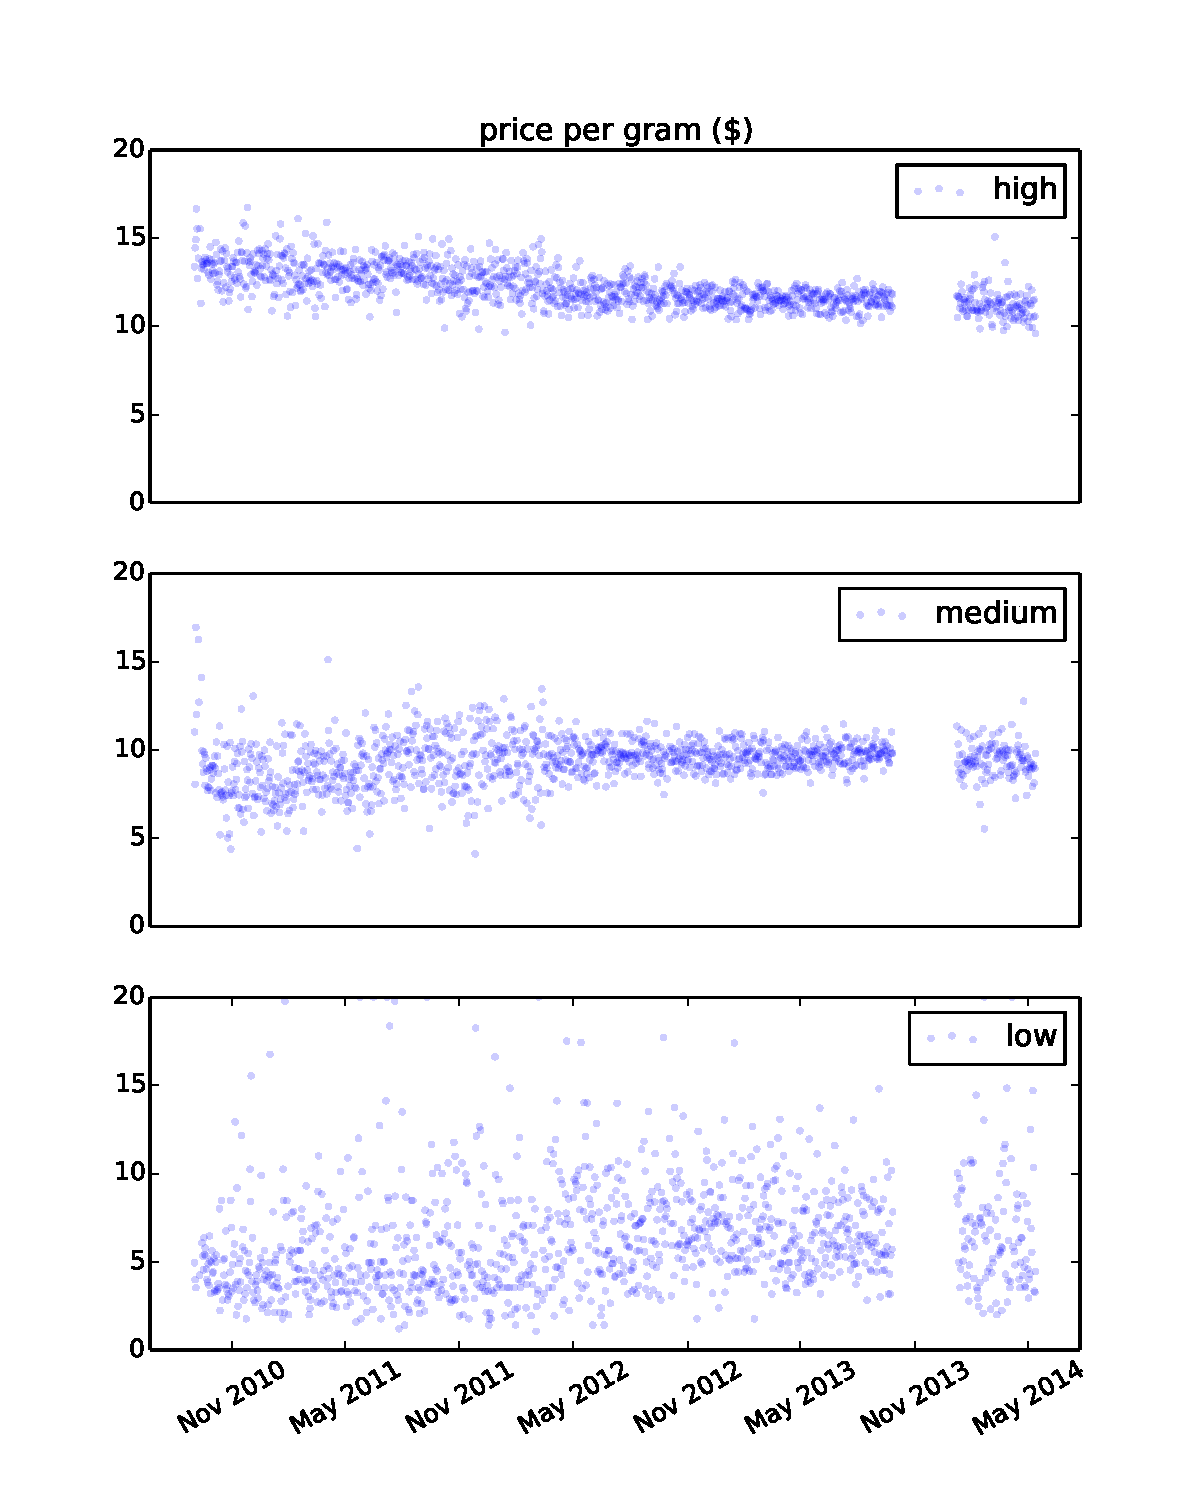
\includegraphics[width=3.5in]{figs/timeseries1.pdf}}
\caption{Time series of daily price per gram for high, medium, and low
quality cannabis.}
\label{timeseries1}
\end{figure}

Figure~\ref{timeseries1} shows the result.  One apparent feature in
these plots is a gap around November 2013.  It's possible that data
collection was not active during this time, or the data might not
be available.  We will consider ways to deal with this missing data
later.
\index{missing values}

Visually, it looks like the price of high quality cannabis is
declining during this period, and the price of medium quality is
increasing.  The price of low quality might also be increasing, but it
is harder to tell, since it seems to be more volatile.  Keep in mind
that quality data is reported by volunteers, so trends over time
might reflect changes in how participants apply these labels.
\index{price}


\section{Linear regression}
\label{timeregress}

Although there are methods specific to time series analysis, for many
problems a simple way to get started is by applying general-purpose
tools like linear regression.  The following function takes a
DataFrame of daily prices and computes a least squares fit, returning
the model and results objects from StatsModels:
\index{DataFrame}
\index{StatsModels}
\index{linear regression}

\begin{verbatim}
def RunLinearModel(daily):
    model = smf.ols('ppg ~ years', data=daily)
    results = model.fit()
    return model, results
\end{verbatim}

Then we can iterate through the qualities and fit a model to
each:

\begin{verbatim}
    for name, daily in dailies.items():
        model, results = RunLinearModel(daily)
        print(name)
        regression.SummarizeResults(results)
\end{verbatim}

Here are the results:

\begin{center}
\begin{tabular}{|l|l|l|c|} \hline
quality & intercept & slope & $R^2$ \\ \hline
high    & 13.450  & -0.708  & 0.444 \\
medium  &  8.879  & 0.283   & 0.050 \\
low     &  5.362  & 0.568   & 0.030 \\
\hline
\end{tabular}
\end{center}

The estimated slopes indicate that the price of high quality cannabis
dropped by about 71 cents per year during the observed interval; for
medium quality it increased by 28 cents per year, and for low quality
it increased by 57 cents per year.  These estimates are all
statistically significant with very small p-values.
\index{p-value}
  \index{significant} \index{statistically significant}

The $R^2$ value for high quality cannabis is 0.44, which means
that time as an explanatory variable accounts for 44\% of the observed
variability in price.  For the other qualities, the change in price
is smaller, and variability in prices is higher, so the values
of $R^2$ are smaller (but still statistically significant).
\index{explanatory variable}
  \index{significant} \index{statistically significant}

The following code plots the observed prices and the fitted values:

\begin{verbatim}
def PlotFittedValues(model, results, label=''):
    years = model.exog[:,1]
    values = model.endog
    thinkplot.Scatter(years, values, s=15, label=label)
    thinkplot.Plot(years, results.fittedvalues, label='model')
\end{verbatim}

As we saw in Section~\ref{implementation}, {\tt model} contains
{\tt exog} and {\tt endog}, NumPy arrays with the exogenous
(explanatory) and endogenous (dependent) variables.
\index{NumPy}
\index{explanatory variable}
\index{dependent variable}
\index{exogenous variable}
\index{endogenous variable}

\begin{figure}
% timeseries.py
\centerline{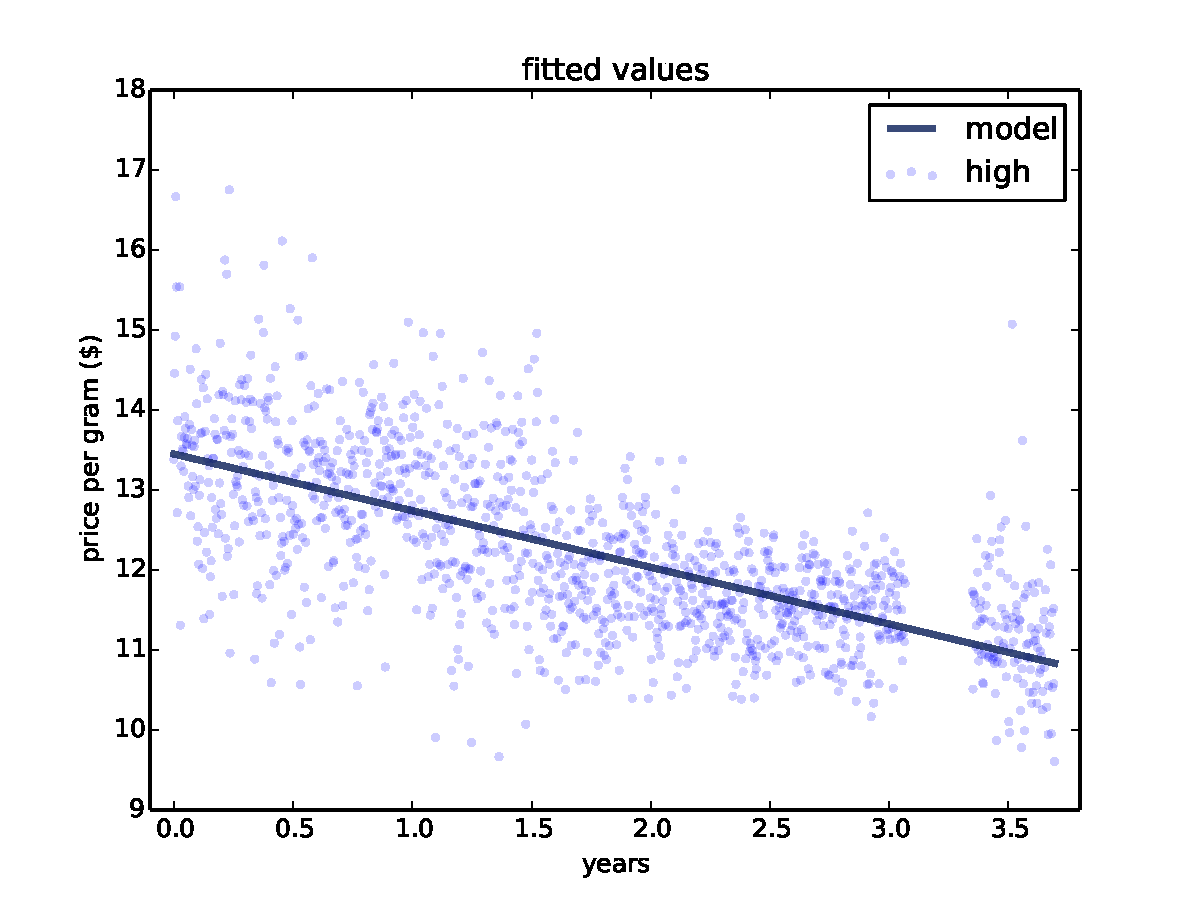
\includegraphics[height=2.5in]{figs/timeseries2.pdf}}
\caption{Time series of daily price per gram for high quality cannabis,
and a linear least squares fit.}
\label{timeseries2}
\end{figure}

{\tt PlotFittedValues} makes a scatter plot of the data points and a line
plot of the fitted values.  Figure~\ref{timeseries2} shows the results
for high quality cannabis.  The model seems like a good linear fit
for the data; nevertheless, linear regression is not the most 
appropriate choice for this data:
\index{model}
\index{fitted values}

\begin{itemize}

\item First, there is no reason to expect the long-term trend to be a
  line or any other simple function.  In general, prices are
  determined by supply and demand, both of which vary over time in
  unpredictable ways.
\index{trend}

\item Second, the linear regression model gives equal weight to all
  data, recent and past.  For purposes of prediction, we should
  probably give more weight to recent data.
\index{weight}

\item Finally, one of the assumptions of linear regression is that the
  residuals are uncorrelated noise.  With time series data, this
  assumption is often false because successive values are correlated.
\index{residuals}

\end{itemize}

The next section presents an alternative that is more appropriate
for time series data.


\section{Moving averages}

Most time series analysis is based on the modeling assumption that the
observed series is the sum of three components:
\index{model}
\index{moving average}

\begin{itemize}

\item Trend: A smooth function that captures persistent changes.
\index{trend}

\item Seasonality: Periodic variation, possibly including daily,
weekly, monthly, or yearly cycles.
\index{seasonality}

\item Noise: Random variation around the long-term trend.
\index{noise}

\end{itemize}

Regression is one way to extract the trend from a series, as we
saw in the previous section.  But if the trend is not a simple
function, a good alternative is a {\bf moving average}.  A moving
average divides the series into overlapping regions, called {\bf windows},
and computes the average of the values in each window.
\index{window}

One of the simplest moving averages is the {\bf rolling mean}, which
computes the mean of the values in each window.  For example, if
the window size is 3, the rolling mean computes the mean of
values 0 through 2, 1 through 3, 2 through 4, etc.
\index{rolling mean}
\index{mean!rolling}

pandas provides \verb"rolling_mean", which takes a Series and a
window size and returns a new Series.
\index{pandas}
\index{Series}

\begin{verbatim}
>>> series = np.arange(10)
array([0, 1, 2, 3, 4, 5, 6, 7, 8, 9])

>>> pandas.rolling_mean(series, 3)
array([ nan,  nan,   1,   2,   3,   4,   5,   6,   7,   8])
\end{verbatim}

The first two values are {\tt nan}; the next value is the mean of
the first three elements, 0, 1, and 2.  The next value is the mean
of 1, 2, and 3.  And so on.

Before we can apply \verb"rolling_mean" to the cannabis data, we
have to deal with missing values.  There are a few days in the
observed interval with no reported transactions for one or more
quality categories, and a period in 2013 when data collection was
not active.
\index{missing values}

In the DataFrames we have used so far, these dates are absent;
the index skips days with no data.  For the analysis that follows,
we need to represent this missing data explicitly.  We can do
that by ``reindexing'' the DataFrame:
 \index{DataFrame}
\index{reindex}

\begin{verbatim}
    dates = pandas.date_range(daily.index.min(), daily.index.max())
    reindexed = daily.reindex(dates)
\end{verbatim}

The first line computes a date range that includes every day from the
beginning to the end of the observed interval.  The second line
creates a new DataFrame with all of the data from {\tt daily}, but
including rows for all dates, filled with {\tt nan}.
\index{interval}
\index{date range}

Now we can plot the rolling mean like this:

\begin{verbatim}
    roll_mean = pandas.rolling_mean(reindexed.ppg, 30)
    thinkplot.Plot(roll_mean.index, roll_mean)
\end{verbatim}

The window size is 30, so each value in \verb"roll_mean" is
the mean of 30 values from {\tt reindexed.ppg}.  
\index{pandas}
\index{window}

\begin{figure}
% timeseries.py
\centerline{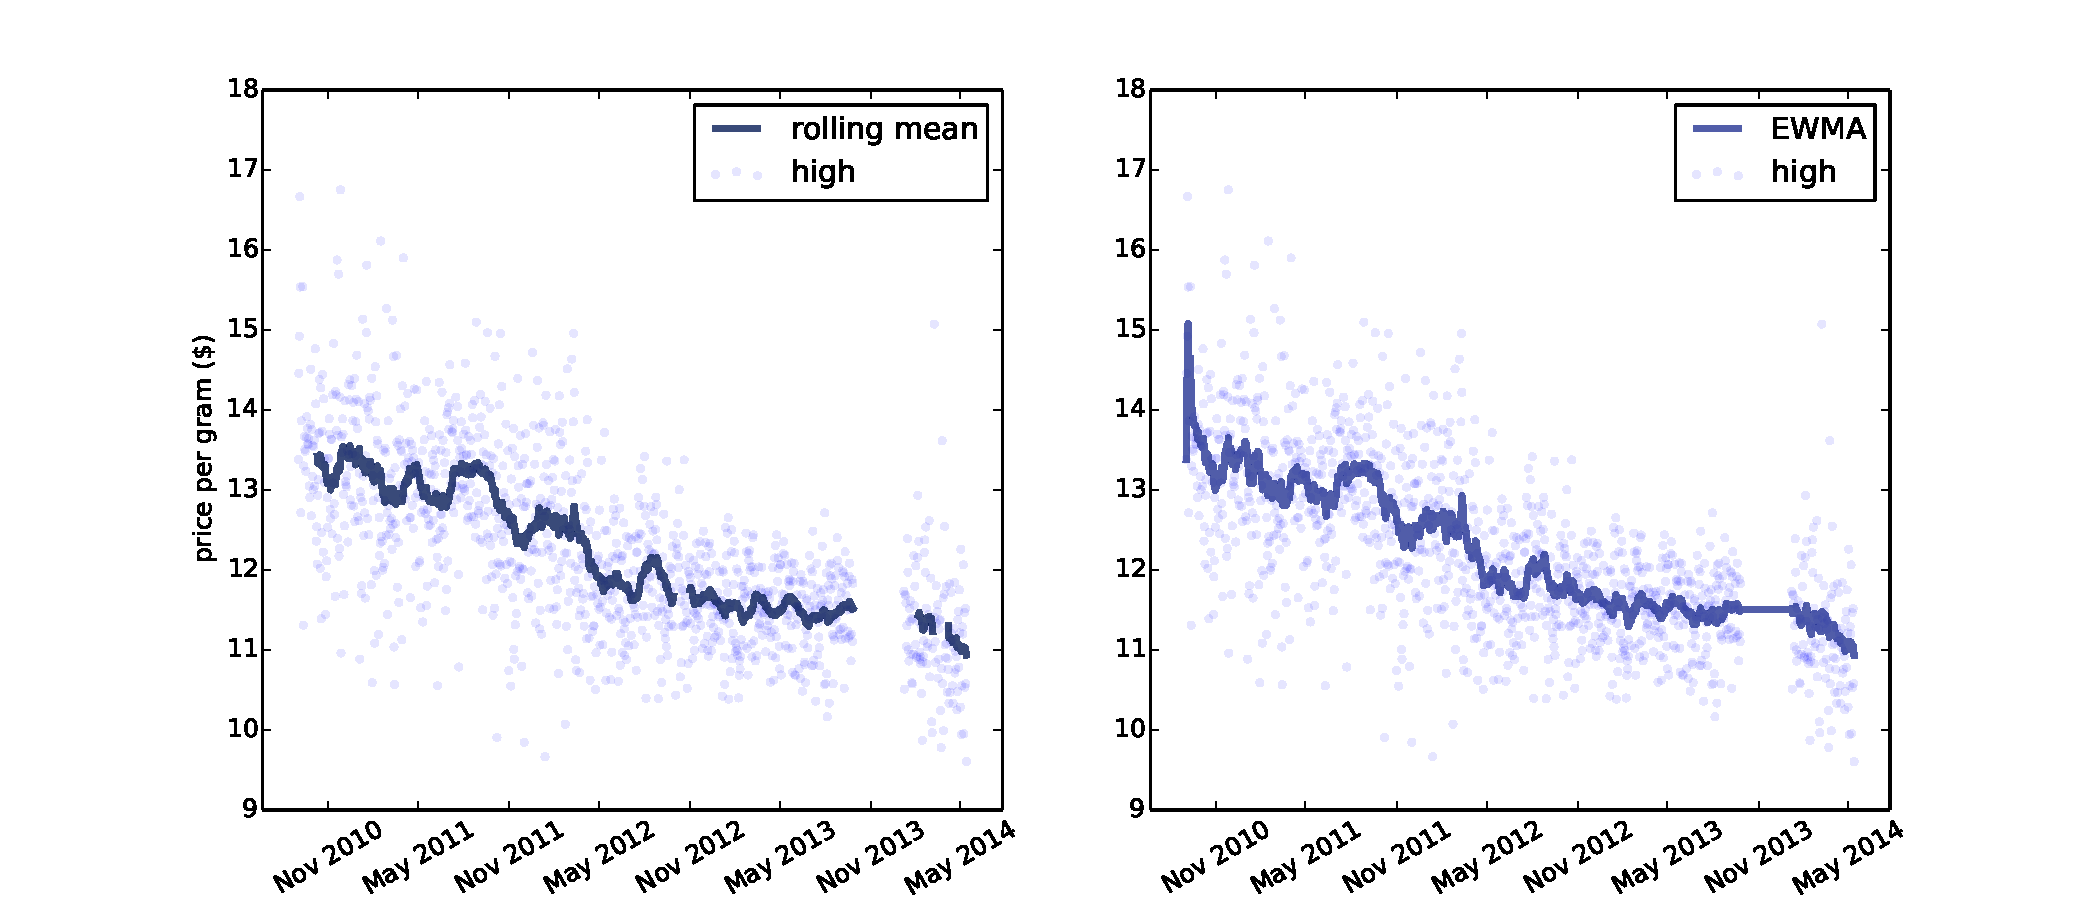
\includegraphics[height=2.5in]{figs/timeseries10.pdf}}
\caption{Daily price and a rolling mean (left) and exponentially-weighted
moving average (right).}
\label{timeseries10}
\end{figure}

Figure~\ref{timeseries10} (left)
shows the result. 
The rolling mean seems to do a good job of smoothing out the noise and
extracting the trend.  The first 29 values are {\tt nan}, and wherever
there's a missing value, it's followed by another 29 {\tt nan}s.
There are ways to fill in these gaps, but they are a minor nuisance.
\index{missing values}
\index{noise}
\index{smoothing}

An alternative is the {\bf exponentially-weighted moving average} (EWMA),
which has two advantages.  First, as the name suggests, it computes
a weighted average where the most recent value has the highest weight
and the weights for previous values drop off exponentially.
Second, the pandas implementation of EWMA handles missing values
better.
\index{reindex}
\index{exponentially-weighted moving average}
\index{EWMA}

\begin{verbatim}
    ewma = pandas.ewma(reindexed.ppg, span=30)
    thinkplot.Plot(ewma.index, ewma)
\end{verbatim}

The {\bf span} parameter corresponds roughly to the window size of
a moving average; it controls how fast the weights drop off, so it
determines the number of points that make a non-negligible contribution
to each average.
\index{span}
\index{window}

Figure~\ref{timeseries10} (right) shows the EWMA for the same data.
It is similar to the rolling mean, where they are both defined,
but it has no missing values, which makes it easier to work with.  The
values are noisy at the beginning of the time series, because they are
based on fewer data points.
\index{missing values}


\section{Missing values}

Now that we have characterized the trend of the time series, the
next step is to investigate seasonality, which is periodic behavior.
Time series data based on human behavior often exhibits daily,
weekly, monthly, or yearly cycles.  In the next section I present
methods to test for seasonality, but they don't work well with
missing data, so we have to solve that problem first.
\index{missing values}
\index{seasonality}

A simple and common way to fill missing data is to use a moving
average.  The Series method {\tt fillna} does just what we want:
\index{Series}
\index{fillna}

\begin{verbatim}
    reindexed.ppg.fillna(ewma, inplace=True)
\end{verbatim}

Wherever {\tt reindexed.ppg} is {\tt nan}, {\tt fillna} replaces
it with the corresponding value from {\tt ewma}.  The {\tt inplace}
flag tells {\tt fillna} to modify the existing Series rather than
create a new one.

A drawback of this method is that it understates the noise in the
series.  We can solve that problem by adding in resampled
residuals:
\index{resampling}
\index{noise}

\begin{verbatim}
    resid = (reindexed.ppg - ewma).dropna()
    fake_data = ewma + thinkstats2.Resample(resid, len(reindexed))
    reindexed.ppg.fillna(fake_data, inplace=True)
\end{verbatim}

% (One note on vocabulary: in this book I am using
%``resampling'' in the statistical sense, which is drawing a random
%sample from a population that is, itself, a sample.  In the context
%of time series analysis, it has another meaning: changing the
%time between measurements in a series.  I don't use the second
%meaning in this book, but you might encounter it.)

{\tt resid} contains the residual values, not including days
when {\tt ppg} is {\tt nan}.  \verb"fake_data" contains the
sum of the moving average and a random sample of residuals.
Finally, {\tt fillna} replaces {\tt nan} with values from
\verb"fake_data".
\index{dropna}
\index{fillna}
\index{NaN}

\begin{figure}
% timeseries.py
\centerline{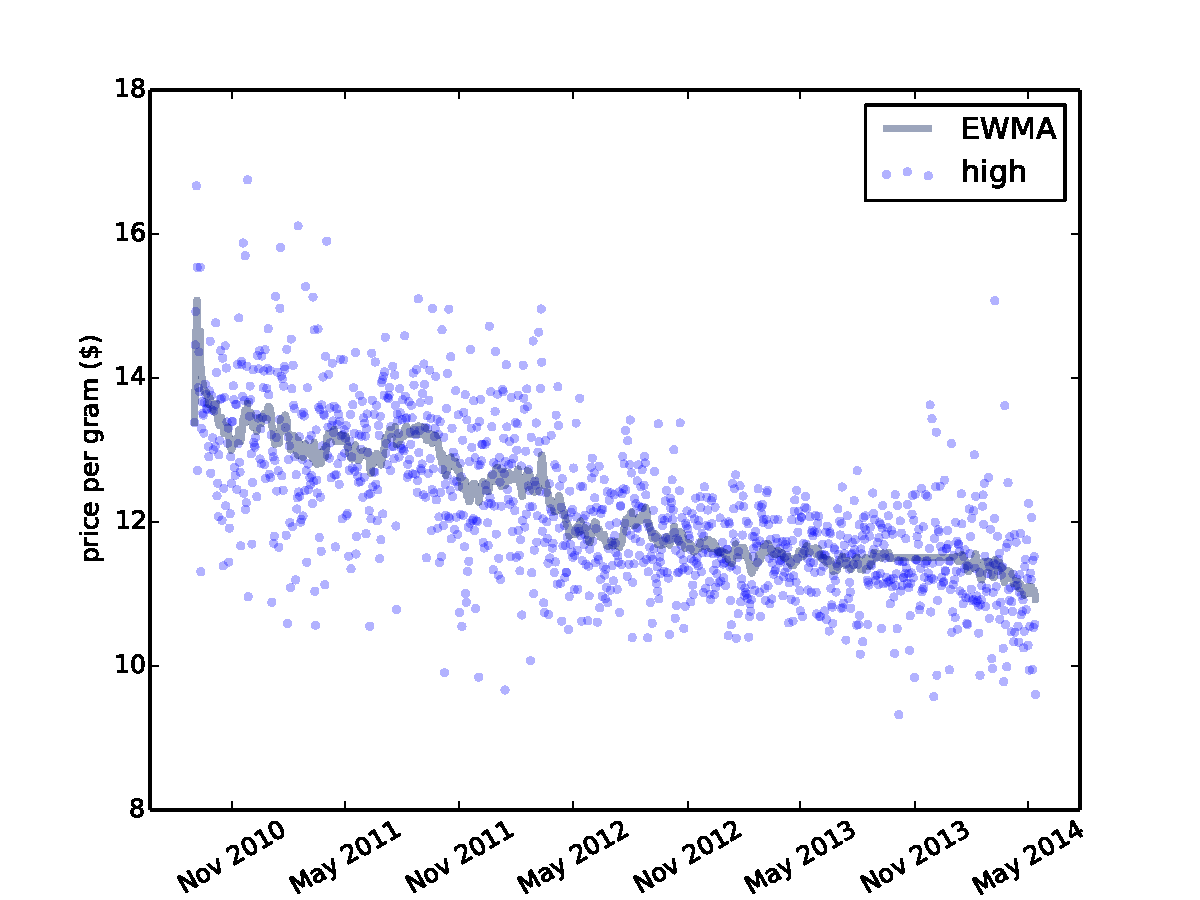
\includegraphics[height=2.5in]{figs/timeseries8.pdf}}
\caption{Daily price with filled data.}
\label{timeseries8}
\end{figure}

Figure~\ref{timeseries8} shows the result.  The filled data is visually
similar to the actual values.  Since the resampled residuals are
random, the results are different every time; later we'll see how
to characterize the error created by missing values.
\index{resampling}
\index{missing values}


\section{Serial correlation}

As prices vary from day to day, you might expect to see patterns.
If the price is high on Monday,
you might expect it to be high for a few more days; and
if it's low, you might expect it to stay low.  A pattern
like this is called {\bf serial
correlation}, because each value is correlated with the next one
in the series.
\index{correlation!serial}
\index{serial correlation}

To compute serial correlation, we can shift the time series
by an interval called a {\bf lag}, and then compute the correlation
of the shifted series with the original:
\index{lag}

\begin{verbatim}
def SerialCorr(series, lag=1):
    xs = series[lag:]
    ys = series.shift(lag)[lag:]
    corr = thinkstats2.Corr(xs, ys)
    return corr
\end{verbatim}

After the shift, the first {\tt lag} values are {\tt nan}, so
I use a slice to remove them before computing {\tt Corr}.
\index{NaN}

%high 0.480121816154
%medium 0.164600078362
%low 0.103373620131

If we apply {\tt SerialCorr} to the raw price data with lag 1, we find
serial correlation 0.48 for the high quality category, 0.16 for
medium and 0.10 for low.  In any time series with a long-term trend,
we expect to see strong serial correlations; for example, if prices
are falling, we expect to see values above the mean in the first
half of the series and values below the mean in the second half.

It is more interesting to see if the correlation persists if you
subtract away the trend.  For example, we can compute the residual
of the EWMA and then compute its serial correlation:
\index{EWMA}

\begin{verbatim}
    ewma = pandas.ewma(reindexed.ppg, span=30)
    resid = reindexed.ppg - ewma
    corr = SerialCorr(resid, 1)
\end{verbatim}

With lag=1, the serial correlations for the de-trended data are
-0.022 for high quality, -0.015 for medium, and 0.036 for low.
These values are small, indicating that there is little or
no one-day serial correlation in this series.
\index{pandas}

To check for weekly, monthly, and yearly seasonality, I ran
the analysis again with different lags.  Here are the results:
\index{seasonality}

\begin{center}
\begin{tabular}{|c|c|c|c|}
\hline
lag & high & medium & low \\ \hline
1 & -0.029 & -0.014 & 0.034 \\
7 & 0.02 & -0.042 & -0.0097 \\
30 & 0.014 & -0.0064 & -0.013 \\
365 & 0.045 & 0.015 & 0.033 \\
\hline
\end{tabular}
\end{center}

In the next section we'll test whether these correlations are
statistically significant (they are not), but at this point we can
tentatively conclude that there are no substantial seasonal patterns
in these series, at least not with these lags.
  \index{significant} \index{statistically significant}


\section{Autocorrelation}

If you think a series might have some serial correlation, but you
don't know which lags to test, you can test them all!  The {\bf
  autocorrelation function} is a function that maps from lag to the
serial correlation with the given lag.  ``Autocorrelation'' is another
name for serial correlation, used more often when the lag is not 1.
\index{autocorrelation function}

StatsModels, which we used for linear regression in
Section~\ref{statsmodels}, also provides functions for time series
analysis, including {\tt acf}, which computes the autocorrelation
function:
\index{StatsModels}

\begin{verbatim}
    import statsmodels.tsa.stattools as smtsa
    acf = smtsa.acf(filled.resid, nlags=365, unbiased=True)
\end{verbatim}

{\tt acf} computes serial correlations with
lags from 0 through {\tt nlags}.  The {\tt unbiased} flag tells
{\tt acf} to correct the estimates for the sample size.  The result
is an array of correlations.  If we select daily prices for high
quality, and extract correlations for lags 1, 7, 30, and 365, we can
confirm that {\tt acf} and {\tt SerialCorr} yield approximately
the same results:
\index{acf}

\begin{verbatim}
>>> acf[0], acf[1], acf[7], acf[30], acf[365]
1.000, -0.029, 0.020, 0.014, 0.044
\end{verbatim}

With {\tt lag=0}, {\tt acf} computes the correlation of the series
with itself, which is always 1.
\index{lag}

\begin{figure}
% timeseries.py
\centerline{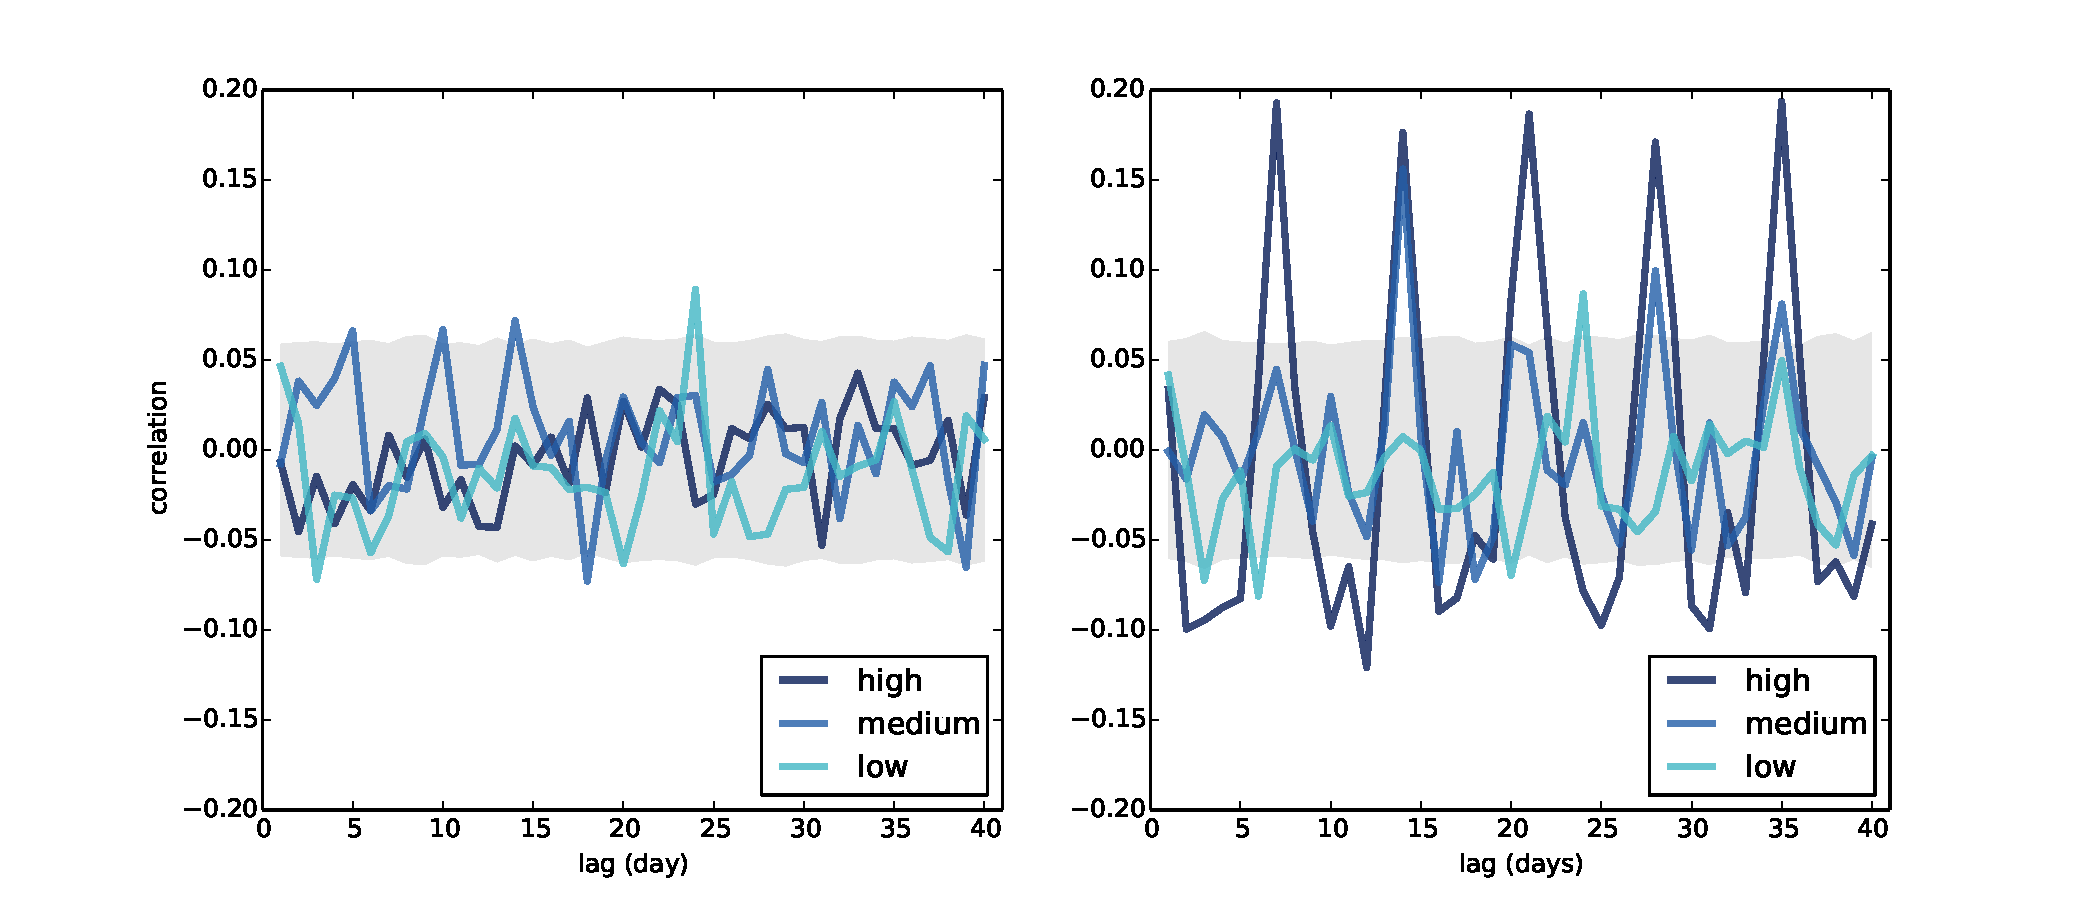
\includegraphics[height=2.5in]{figs/timeseries9.pdf}}
\caption{Autocorrelation function for daily prices (left), and
daily prices with a simulated weekly seasonality (right).}
\label{timeseries9}
\end{figure}

Figure~\ref{timeseries9} (left) shows autocorrelation functions for
the three quality categories, with {\tt nlags=40}.  The gray region
shows the normal variability we would expect if there is no actual
autocorrelation; anything that falls outside this range is
statistically significant, with a p-value less than 5\%.  Since
the false positive rate is 5\%, and
we are computing 120 correlations (40 lags for each of 3 times series),
we expect to see about 6 points outside this region.  In fact, there
are 7.  We conclude that there are no autocorrelations
in these series that could not be explained by chance.
\index{p-value}
  \index{significant} \index{statistically significant}
\index{false positive}

I computed the gray regions by resampling the residuals.  You
can see my code in {\tt timeseries.py}; the function is called
{\tt SimulateAutocorrelation}.
\index{resampling}

To see what the autocorrelation function looks like when there is a
seasonal component, I generated simulated data by adding a weekly
cycle.  Assuming that demand for cannabis is higher on weekends, we
might expect the price to be higher.  To simulate this effect, I
select dates that fall on Friday or Saturday and add a random amount
to the price, chosen from a uniform distribution from \$0 to \$2.
\index{simulation}
\index{uniform distribution}
\index{distribution!uniform}

\begin{verbatim}
def AddWeeklySeasonality(daily):
    frisat = (daily.index.dayofweek==4) | (daily.index.dayofweek==5)
    fake = daily.copy()
    fake.ppg[frisat] += np.random.uniform(0, 2, frisat.sum())
    return fake
\end{verbatim}

{\tt frisat} is a boolean Series, {\tt True} if the day of the
week is Friday or Saturday.  {\tt fake} is a new DataFrame, initially
a copy of {\tt daily}, which we modify by adding random values
to {\tt ppg}.  {\tt frisat.sum()} is the total number of Fridays
and Saturdays, which is the number of random values we have to
generate.
\index{DataFrame}
\index{Series}
\index{boolean}

Figure~\ref{timeseries9} (right) shows autocorrelation functions for
prices with this simulated seasonality.  As expected, the
correlations are highest when the lag is a multiple of 7.  For
high and medium quality, the new correlations are statistically
significant.  For low quality they are not, because residuals in this
category are large; the effect would have to be bigger
to be visible through the noise.
  \index{significant} \index{statistically significant}
\index{residuals}
\index{lag}


\section{Prediction}  

Time series analysis can be used to investigate, and sometimes
explain, the behavior of systems that vary in time.  It can also
make predictions.
\index{prediction}

The linear regressions we used in Section~\ref{timeregress} can be
used for prediction.  The RegressionResults class provides {\tt
  predict}, which takes a DataFrame containing the explanatory
variables and returns a sequence of predictions.  Here's the code:
\index{explanatory variable}
\index{linear regression}

\begin{verbatim}
def GenerateSimplePrediction(results, years):
    n = len(years)
    inter = np.ones(n)
    d = dict(Intercept=inter, years=years)
    predict_df = pandas.DataFrame(d)
    predict = results.predict(predict_df)
    return predict
\end{verbatim}

{\tt results} is a RegressionResults object; {\tt years} is the
sequence of time values we want predictions for.  The function
constructs a DataFrame, passes it to {\tt predict}, and
returns the result.
\index{pandas}
\index{DataFrame}

If all we want is a single, best-guess prediction, we're done.  But
for most purposes it is important to quantify error.  In other words,
we want to know how accurate the prediction is likely to be.

There are three sources of error we should take into account:

\begin{itemize}

\item Sampling error: The prediction is based on estimated
parameters, which depend on random variation
in the sample.  If we run the experiment again, we expect
the estimates to vary.
\index{sampling error}
\index{parameter}

\item Random variation:  Even if the estimated parameters are
perfect, the observed data varies randomly around the long-term
trend, and we expect this variation to continue in the future.
\index{noise}

\item Modeling error: We have already seen evidence that the long-term
trend is not linear, so predictions based on a linear model will
eventually fail.  
\index{modeling error}

\end{itemize}

Another source of error to consider is unexpected future events.
Agricultural prices are affected by weather, and all prices are
affected by politics and law.  As I write this, cannabis is legal in
two states and legal for medical purposes in 20 more.  If more states
legalize it, the price is likely to go down.  But if
the federal government cracks down, the price might go up.

Modeling errors and unexpected future events are hard to quantify.
Sampling error and random variation are easier to deal with, so we'll
do that first.

To quantify sampling error, I use resampling, as we did in
Section~\ref{regest}.  As always, the goal is to use the actual
observations to simulate what would happen if we ran the experiment
again.  The simulations are based on the assumption that the estimated
parameters are correct, but the random residuals could have been
different.  Here is a function that runs the simulations:
\index{resampling}

\begin{verbatim}
def SimulateResults(daily, iters=101):
    model, results = RunLinearModel(daily)
    fake = daily.copy()
    
    result_seq = []
    for i in range(iters):
        fake.ppg = results.fittedvalues + Resample(results.resid)
        _, fake_results = RunLinearModel(fake)
        result_seq.append(fake_results)

    return result_seq
\end{verbatim}

{\tt daily} is a DataFrame containing the observed prices;
{\tt iters} is the number of simulations to run.
\index{DataFrame}
\index{price}

{\tt SimulateResults} uses {\tt RunLinearModel}, from
Section~\ref{timeregress}, to estimate the slope and intercept
of the observed values.

Each time through the loop, it generates a ``fake'' dataset by
resampling the residuals and adding them to the fitted values.  Then
it runs a linear model on the fake data and stores the RegressionResults
object.
\index{model}
\index{residuals}

The next step is to use the simulated results to generate predictions:

\begin{verbatim}
def GeneratePredictions(result_seq, years, add_resid=False):
    n = len(years)
    d = dict(Intercept=np.ones(n), years=years, years2=years**2)
    predict_df = pandas.DataFrame(d)
    
    predict_seq = []
    for fake_results in result_seq:
        predict = fake_results.predict(predict_df)
        if add_resid:
            predict += thinkstats2.Resample(fake_results.resid, n)
        predict_seq.append(predict)

    return predict_seq
\end{verbatim}

{\tt GeneratePredictions} takes the sequence of results from the
previous step, as well as {\tt years}, which is a sequence of
floats that specifies the interval to generate predictions for,
and \verb"add_resid", which indicates whether it should add resampled
residuals to the straight-line prediction.
{\tt GeneratePredictions} iterates through the sequence of
RegressionResults and generates a sequence of predictions.
\index{resampling}

\begin{figure}
% timeseries.py
\centerline{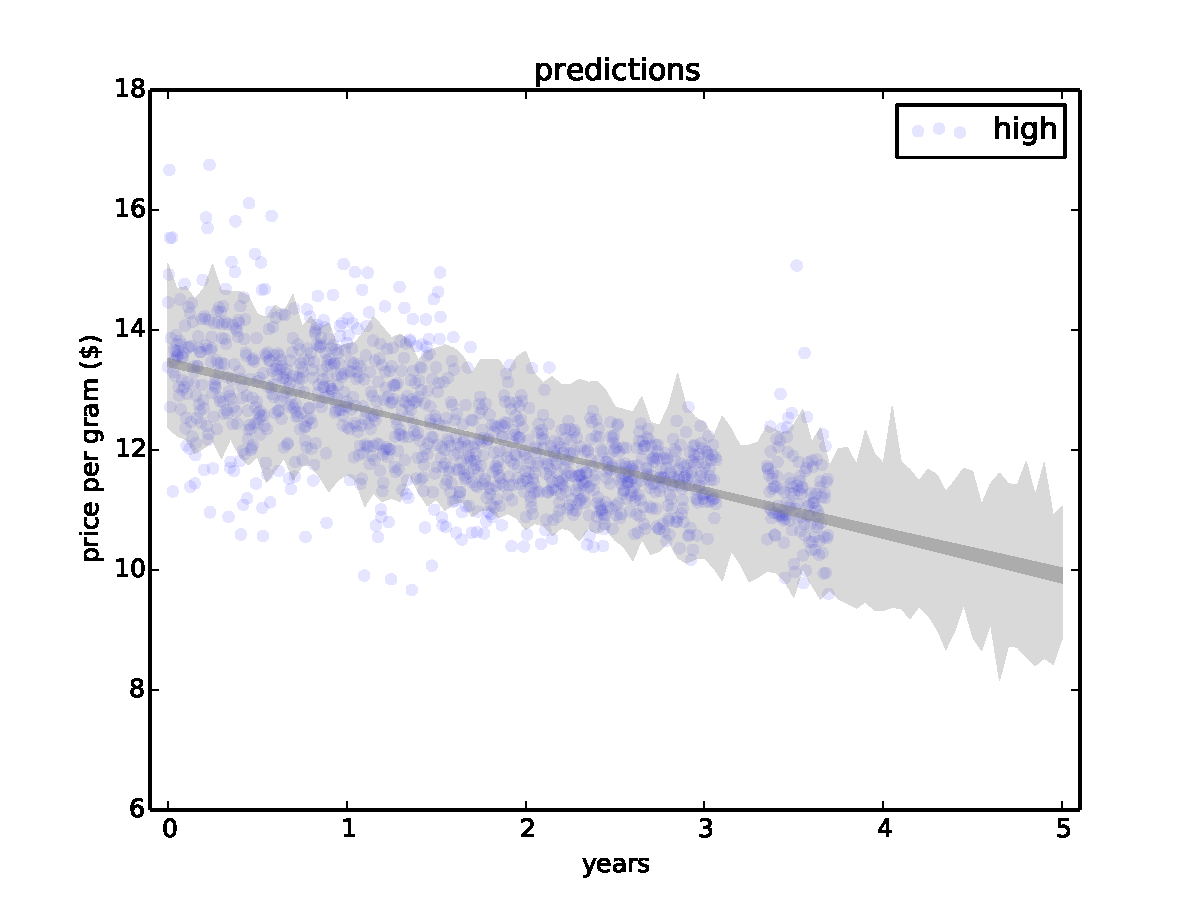
\includegraphics[height=2.5in]{figs/timeseries4.pdf}}
\caption{Predictions based on linear fits, showing variation due
to sampling error and prediction error.}
\label{timeseries4}
\end{figure}

Finally, here's the code that plots a 90\% confidence interval for
the predictions:
\index{confidence interval}

\begin{verbatim}
def PlotPredictions(daily, years, iters=101, percent=90):
    result_seq = SimulateResults(daily, iters=iters)
    p = (100 - percent) / 2
    percents = p, 100-p

    predict_seq = GeneratePredictions(result_seq, years, True)
    low, high = thinkstats2.PercentileRows(predict_seq, percents)
    thinkplot.FillBetween(years, low, high, alpha=0.3, color='gray')

    predict_seq = GeneratePredictions(result_seq, years, False)
    low, high = thinkstats2.PercentileRows(predict_seq, percents)
    thinkplot.FillBetween(years, low, high, alpha=0.5, color='gray')
\end{verbatim}

{\tt PlotPredictions} calls {\tt GeneratePredictions} twice: once
with \verb"add_resid=True" and again with \verb"add_resid=False".
It uses {\tt PercentileRows} to select the 5th and 95th percentiles
for each year, then plots a gray region between these bounds.
\index{FillBetween}

Figure~\ref{timeseries4} shows the result.
The dark gray region represents a 90\% confidence interval for
the sampling error; that is, uncertainty about the estimated
slope and intercept due to sampling.
\index{sampling error}

The lighter region shows
a 90\% confidence interval for prediction error, which is the
sum of sampling error and random variation.
\index{noise}

These regions quantify sampling error and random variation, but
not modeling error.  In general modeling error is hard to quantify,
but in this case we can address at least one source of error,
unpredictable external events.
\index{modeling error}

The regression model is based on the assumption that the system
is {\bf stationary}; that is, that the parameters of the model
don't change over time.
Specifically, it assumes that the slope and
intercept are constant, as well as the distribution of residuals.
\index{stationary model}
\index{parameter}

But looking at the moving averages in Figure~\ref{timeseries10}, it
seems like the slope changes at least once during the observed
interval, and the variance of the residuals seems bigger in the first
half than the second.
\index{slope}

As a result, the parameters we get depend on the interval we
observe.  To see how much effect this has on the predictions,
we can extend {\tt SimulateResults} to use intervals of observation
with different start and end dates.  My implementation is in
{\tt timeseries.py}.
\index{simulation}

\begin{figure}
% timeseries.py
\centerline{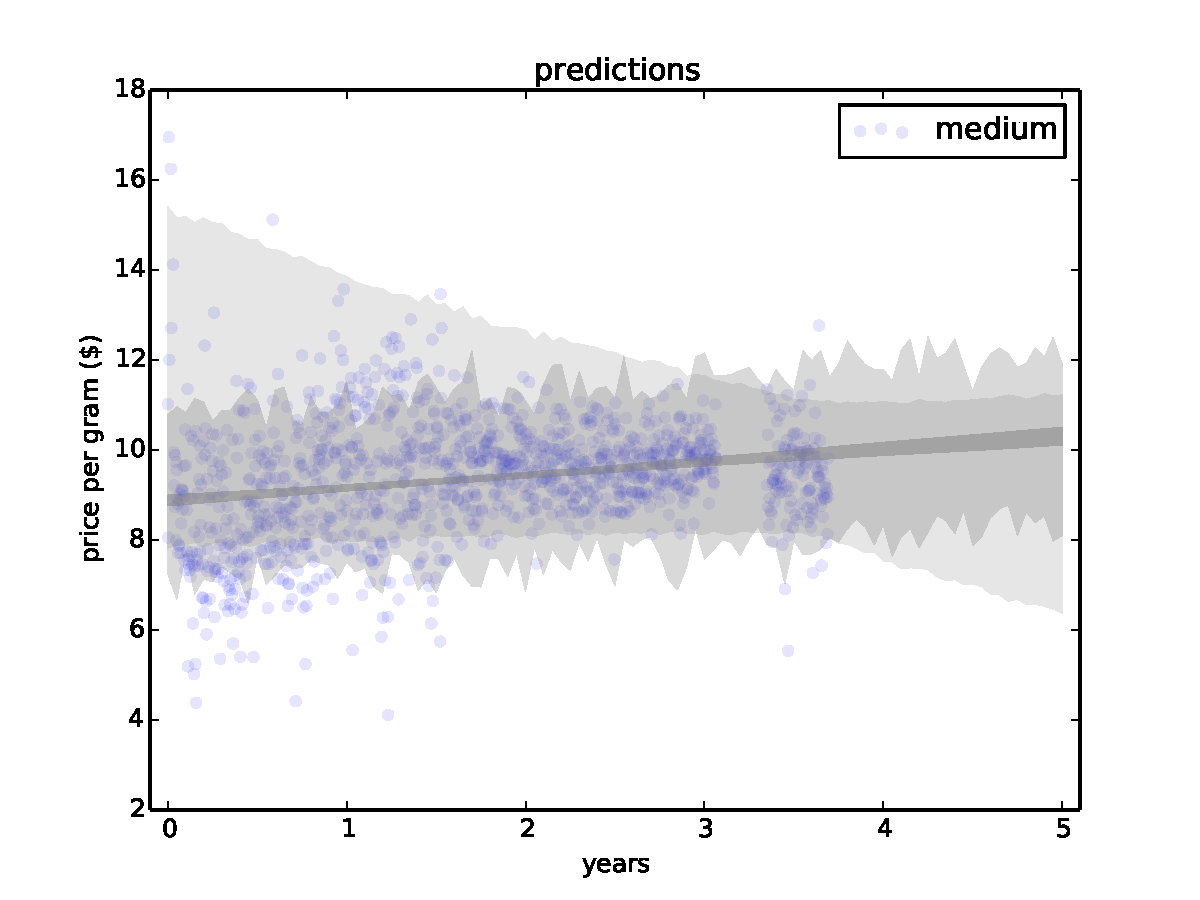
\includegraphics[height=2.5in]{figs/timeseries5.pdf}}
\caption{Predictions based on linear fits, showing
variation due to the interval of observation.}
\label{timeseries5}
\end{figure}

Figure~\ref{timeseries5} shows the result for the medium quality
category.  The lightest gray area shows a confidence interval that
includes uncertainty due to sampling error, random variation, and
variation in the interval of observation.
\index{confidence interval}
\index{interval}

The model based on the entire interval has positive slope, indicating
that prices were increasing.  But the most recent interval shows signs
of decreasing prices, so models based on the most recent data have
negative slope.  As a result, the widest predictive interval includes
the possibility of decreasing prices over the next year.
\index{model}


\section{Further reading}

Time series analysis is a big topic; this chapter has only scratched
the surface.  An important tool for working with time series data
is autoregression, which I did not cover here, mostly because it turns
out not to be useful for the example data I worked with.
\index{time series}

But once you
have learned the material in this chapter, you are well prepared
to learn about autoregression.  One resource I recommend is
Philipp Janert's book, {\it Data Analysis with Open Source Tools},
O'Reilly Media, 2011.  His chapter on time series analysis picks up
where this one leaves off.
\index{Janert, Philipp}


\section{Exercises}

My solution to these exercises is in \verb"chap12soln.py".

\begin{exercise}
The linear model I used in this chapter has the obvious drawback
that it is linear, and there is no reason to expect prices to
change linearly over time.
We can add flexibility to the model by adding a quadratic term,
as we did in Section~\ref{nonlinear}.  
\index{nonlinear}
\index{linear model}
\index{quadratic model}

Use a quadratic model to fit the time series of daily prices,
and use the model to generate predictions.  You will have to
write a version of {\tt RunLinearModel} that runs that quadratic
model, but after that you should be able to reuse code in
{\tt timeseries.py} to generate predictions.
\index{prediction}

\end{exercise}

\begin{exercise}
Write a definition for a class named {\tt SerialCorrelationTest}
that extends {\tt HypothesisTest} from Section~\ref{hypotest}.
It should take a series and a lag as data, compute the serial
correlation of the series with the given lag, and then compute
the p-value of the observed correlation.
\index{HypothesisTest}
\index{p-value}
\index{lag}

Use this class to test whether the serial correlation in raw
price data is statistically significant.  Also test the residuals
of the linear model and (if you did the previous exercise),
the quadratic model.
\index{quadratic model}
  \index{significant} \index{statistically significant}

\end{exercise}

\begin{exercise}
There are several ways to extend the EWMA model to generate predictions.
One of the simplest is something like this:
\index{EWMA}

\begin{enumerate}

\item Compute the EWMA of the time series and use the last point
as an intercept, {\tt inter}.

\item Compute the EWMA of differences between successive elements in
the time series and use the last point as a slope, {\tt slope}.
\index{slope}

\item To predict values at future times, compute {\tt inter + slope * dt},
where {\tt dt} is the difference between the time of the prediction and
the time of the last observation.
\index{prediction}

\end{enumerate}

Use this method to generate predictions for a year after the last
observation.  A few hints:

\begin{itemize}

\item Use {\tt timeseries.FillMissing} to fill in missing values
before running this analysis.  That way the time between consecutive
elements is consistent.
\index{missing values}

\item Use {\tt Series.diff} to compute differences between successive
elements.
\index{Series}

\item Use {\tt reindex} to extend the DataFrame index into the future.
\index{reindex}

\item Use {\tt fillna} to put your predicted values into the DataFrame.
\index{fillna}

\end{itemize}

\end{exercise}


\section{Glossary}

\begin{itemize}

\item time series: A dataset where each value is associated with
a timestamp, often a series of measurements and the times they
were collected.
\index{time series}

\item window: A sequence of consecutive values in a time series,
often used to compute a moving average.
\index{window}

\item moving average: One of several statistics intended to estimate
the underlying trend in a time series by computing averages (of
some kind) for a series of overlapping windows.
\index{moving average}

\item rolling mean: A moving average based on the mean value in
each window.
\index{rolling mean}

\item exponentially-weighted moving average (EWMA): A moving
average based on a weighted mean that gives the highest weight
to the most recent values, and exponentially decreasing weights
to earlier values. \index{exponentially-weighted moving average} \index{EWMA}

\item span: A parameter of EWMA that determines how quickly the
weights decrease.
\index{span}

\item serial correlation: Correlation between a time series and
a shifted or lagged version of itself.
\index{serial correlation}

\item lag: The size of the shift in a serial correlation or
autocorrelation.
\index{lag}

\item autocorrelation: A more general term for a serial correlation
with any amount of lag.
\index{autocorrelation function}

\item autocorrelation function: A function that maps from lag to
serial correlation.

\item stationary: A model is stationary if the parameters and the
distribution of residuals does not change over time.
\index{model}
\index{stationary model}

\end{itemize}



\chapter{Survival analysis}

{\bf Survival analysis} is a way to describe how long things last.
It is often used to study human lifetimes, but it
also applies to ``survival'' of mechanical and electronic components, or
more generally to intervals in time before an event.
\index{survival analysis}
\index{mechanical component}
\index{electrical component}

If someone you know has been diagnosed with a life-threatening
disease, you might have seen a ``5-year survival rate,'' which
is the probability of surviving five years after diagnosis.  That
estimate and related statistics are the result of survival analysis.
\index{survival rate}

The code in this chapter is in {\tt survival.py}.  For information
about downloading and working with this code, see Section~\ref{code}.


\section{Survival curves}
\label{survival}

The fundamental concept in survival analysis is the {\bf survival
  curve}, $S(t)$, which is a function that maps from a duration, $t$, to the
probability of surviving longer than $t$.  If you know the distribution
of durations, or ``lifetimes'', finding the survival curve is easy;
it's just the complement of the CDF: \index{survival curve}
%
\[ S(t) = 1 - \CDF(t) \]
%
where $CDF(t)$ is the probability of a lifetime less than or equal
to $t$.
\index{complementary CDF} \index{CDF!complementary} \index{CCDF}

For example, in the NSFG dataset, we know the duration of 11189
complete pregnancies.  We can read this data and compute the CDF:
\index{pregnancy length}

\begin{verbatim}
    preg = nsfg.ReadFemPreg()
    complete = preg.query('outcome in [1, 3, 4]').prglngth
    cdf = thinkstats2.Cdf(complete, label='cdf')
\end{verbatim}

The outcome codes {\tt 1, 3, 4} indicate live birth, stillbirth,
and miscarriage.  For this analysis I am excluding induced abortions,
ectopic pregnancies, and pregnancies that were in progress when
the respondent was interviewed.

The DataFrame method {\tt query} takes a boolean expression and
evaluates it for each row, selecting the rows that yield True.
\index{DataFrame}
\index{boolean}
\index{query}

\begin{figure}
% survival.py
\centerline{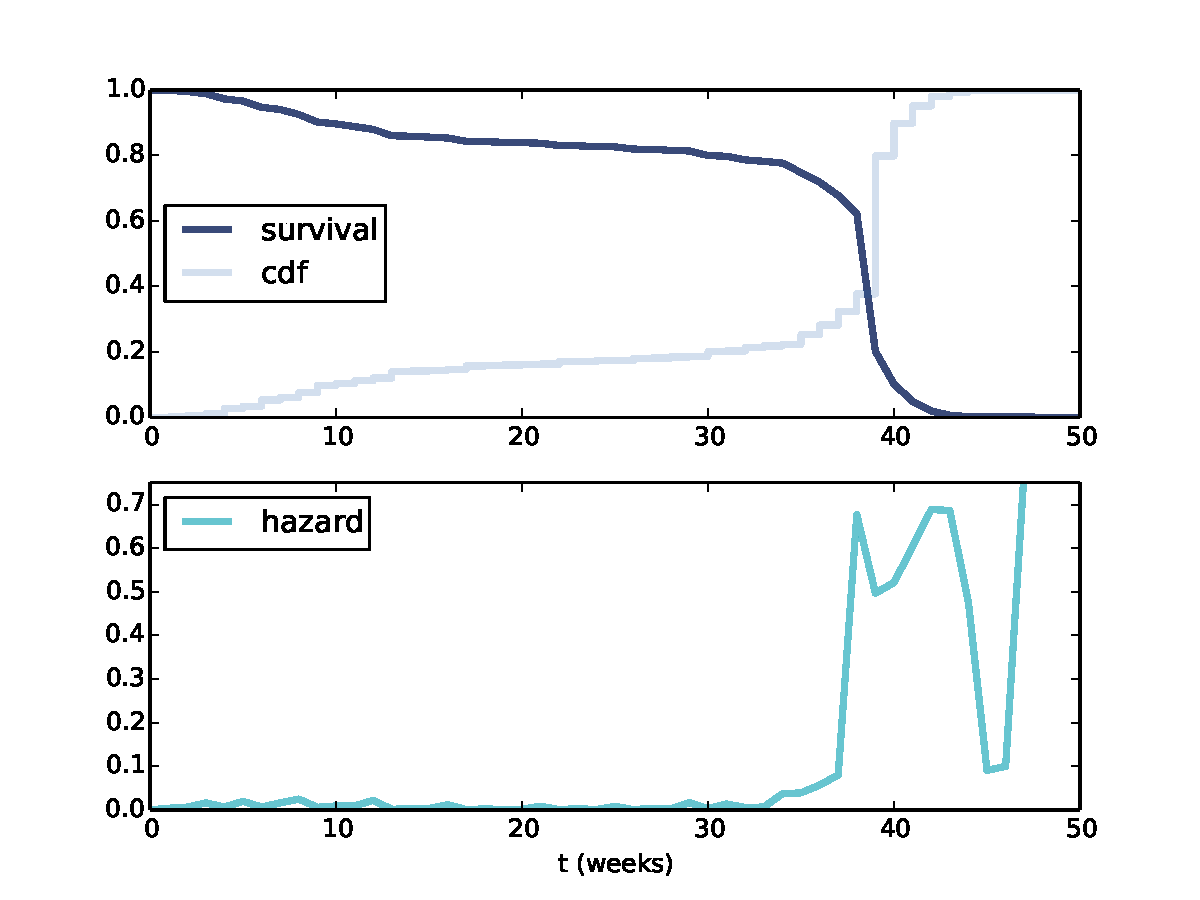
\includegraphics[height=3.0in]{figs/survival1.pdf}}
\caption{Cdf and survival curve for pregnancy length (top),
hazard curve (bottom).}
\label{survival1}
\end{figure}

Figure~\ref{survival1} (top) shows the CDF of pregnancy length
and its complement, the survival curve.  To represent the
survival curve, I define an object that wraps a Cdf and 
adapts the interface:
\index{Cdf}
\index{pregnancy length}
\index{SurvivalFunction}

\begin{verbatim}
class SurvivalFunction(object):
    def __init__(self, cdf, label=''):
        self.cdf = cdf
        self.label = label or cdf.label

    @property
    def ts(self):
        return self.cdf.xs

    @property
    def ss(self):
        return 1 - self.cdf.ps
\end{verbatim}

{\tt SurvivalFunction} provides two properties: {\tt ts}, which
is the sequence of lifetimes, and {\tt ss}, which is the survival
curve.  In Python, a ``property'' is a method that can be
invoked as if it were a variable.

We can instantiate a {\tt SurvivalFunction} by passing
the CDF of lifetimes:
\index{property}

\begin{verbatim}
    sf = SurvivalFunction(cdf)
\end{verbatim}

{\tt SurvivalFunction} also provides \verb"__getitem__" and
{\tt Prob}, which evaluates the survival curve:

\begin{verbatim}
# class SurvivalFunction

    def __getitem__(self, t):
        return self.Prob(t)

    def Prob(self, t):
        return 1 - self.cdf.Prob(t)
\end{verbatim}

For example, {\tt sf[13]} is the fraction of pregnancies that
proceed past the first trimester:
\index{trimester}

\begin{verbatim}
>>> sf[13]
0.86022
>>> cdf[13]
0.13978
\end{verbatim}

About 86\% of pregnancies proceed past the first trimester;
about 14\% do not.

{\tt SurvivalFunction} provides {\tt Render}, so we can
plot {\tt sf} using the functions in {\tt thinkplot}:
\index{thinkplot}

\begin{verbatim}
    thinkplot.Plot(sf)
\end{verbatim}

Figure~\ref{survival1} (top) shows the result.  The curve is nearly
flat between 13 and 26 weeks, which shows that few pregnancies
end in the second trimester.  And the curve is steepest around 39
weeks, which is the most common pregnancy length.
\index{pregnancy length}


\section{Hazard function}
\label{hazard}

From the survival curve we can derive the {\bf hazard function};
for pregnancy lengths, the hazard function maps from a time, $t$, to
the fraction of pregnancies that continue until $t$ and then end at
$t$.  To be more precise:
%
\[ \lambda(t) = \frac{S(t) - S(t+1)}{S(t)} \]
%
The numerator is the fraction of lifetimes that end at $t$, which
is also $\PMF(t)$.
\index{hazard function}

{\tt SurvivalFunction} provides {\tt MakeHazard}, which calculates
the hazard function:

\begin{verbatim}
# class SurvivalFunction

    def MakeHazard(self, label=''):
        ss = self.ss
        lams = {}
        for i, t in enumerate(self.ts[:-1]):
            hazard = (ss[i] - ss[i+1]) / ss[i]
            lams[t] = hazard

        return HazardFunction(lams, label=label)
\end{verbatim}

The {\tt HazardFunction} object is a wrapper for a pandas
Series:
\index{pandas}
\index{Series}
\index{wrapper}

\begin{verbatim}
class HazardFunction(object):

    def __init__(self, d, label=''):
        self.series = pandas.Series(d)
        self.label = label
\end{verbatim}

{\tt d} can be a dictionary or any other type that can initialize
a Series, including another Series.  {\tt label} is a string used
to identify the HazardFunction when plotted.
\index{HazardFunction}

{\tt HazardFunction} provides \verb"__getitem__", so we can evaluate
it like this:

\begin{verbatim}
>>> hf = sf.MakeHazard()
>>> hf[39]
0.49689
\end{verbatim}

So of all pregnancies that proceed until week 39, about
50\% end in week 39.

Figure~\ref{survival1} (bottom) shows the hazard function for
pregnancy lengths.  For times after week 42, the hazard function
is erratic because it is based on a small number of cases.
Other than that the shape of the curve is as expected: it is
highest around 39 weeks, and a little higher in the first
trimester than in the second.
\index{pregnancy length}

The hazard function is useful in its own right, but it is also an
important tool for estimating survival curves, as we'll see in the
next section.


\section{Inferring survival curves}

If someone gives you the CDF of lifetimes, it is easy to compute the
survival and hazard functions.  But in many real-world
scenarios, we can't measure the distribution of lifetimes directly.
We have to infer it.
\index{survival curve}
\index{CDF}

For example, suppose you are following a group of patients to see how
long they survive after diagnosis.  Not all patients are diagnosed on
the same day, so at any point in time, some patients have survived
longer than others.  If some patients have died, we know their
survival times.  For patients who are still alive, we don't know
survival times, but we have a lower bound.
\index{diagnosis}

If we wait until all patients are dead, we can compute the survival
curve, but if we are evaluating the effectiveness of a new treatment,
we can't wait that long!  We need a way to estimate survival curves
using incomplete information.
\index{incomplete information}

As a more cheerful example, I will use NSFG data to quantify how
long respondents ``survive'' until they get married for the
first time.  The range of respondents' ages is 14 to 44 years, so
the dataset provides a snapshot of women at different stages in their
lives.
\index{marital status}

For women who have been married, the dataset includes the date
of their first marriage and their age at the time.
For women who have not been married, we know their age when interviewed,
but have no way of knowing when or if they will get married.
\index{age}

Since we know the age at first marriage for {\em some} women, it
might be tempting to exclude the rest and compute the CDF of
the known data.  That is a bad idea.  The result would
be doubly misleading: (1) older women would be overrepresented,
because they are more likely to be married when interviewed,
and (2) married women would be overrepresented!  In fact, this
analysis would lead to the conclusion that all women get married,
which is obviously incorrect.


\section{Kaplan-Meier estimation}

In this example it is not only desirable but necessary to include
observations of unmarried women, which brings us to one of the central
algorithms in survival analysis, {\bf Kaplan-Meier estimation}.
\index{Kaplan-Meier estimation}

The general idea is that we can use the data to estimate the hazard
function, then convert the hazard function to a survival curve.
To estimate the hazard function, we consider, for each age,
(1) the number of women who got married at that age and (2) the number
of women ``at risk'' of getting married, which includes all women
who were not married at an earlier age.
\index{hazard function}
\index{at risk}

Here's the code:

\begin{verbatim}
def EstimateHazardFunction(complete, ongoing, label=''):

    n = len(complete)
    hist_complete = thinkstats2.Hist(complete)
    sf_complete = SurvivalFunction(thinkstats2.Cdf(complete))

    m = len(ongoing)
    sf_ongoing = SurvivalFunction(thinkstats2.Cdf(ongoing))

    lams = {}
    for t, ended in sorted(hist_complete.Items()):
        at_risk = ended + n * sf_complete[t] + m * sf_ongoing[t]
        lams[t] = ended / at_risk

    return HazardFunction(lams, label=label)
\end{verbatim}

{\tt complete} is the set of complete observations; in this case,
the ages when respondents got married.  {\tt ongoing} is the set
of incomplete observations; that is, the ages of unmarried women
when they were interviewed.

First, we precompute \verb"hist_complete", which is the Hist
of ages when women were married, \verb"sf_complete", the
survival curve for married women, and \verb"sf_ongoing",
the survival curve for unmarried women.
\index{Hist}
\index{survival curve}

The loop iterates through the ages when respondents got married.
For each value of {\tt t}, we have {\tt ended}, which is the number
of women who got married at age {\tt t}.  Then we compute
the number of women ``at risk'', which is the sum of:

\begin{itemize}

\item {\tt ended}, the number of respondents married at age {\tt t},

\item \verb"n * sf_complete[t]", the number of respondents
married after age {\tt t}.

\item \verb"m * sf_ongoing[t]", the number of unmarried respondents
interviewed after {\tt t}, and therefore known not to
have been married at or before {\tt t}.

\end{itemize}

The estimated value of the hazard function at {\tt t} is the ratio of
{\tt ended} to \verb"at_risk".

{\tt lams} is a dictionary that maps
from $t$ to $\lambda(t)$.  The result is a {\tt HazardFunction}
object.
\index{HazardFunction}


\section{The marriage curve}

To test this function, we have to do some data cleaning and
transformation.  The NSFG variables we need are:
\index{marital status}

\begin{itemize}

\item {\tt cmbirth}: The respondent's date of birth, known for
all respondents.
\index{date of birth}

\item {\tt cmintvw}: The date the respondent was interviewed,
known for all respondents.

\item {\tt cmmarrhx}: The date the respondent was first married,
if applicable and known.

\item {\tt evrmarry}: 1 if the respondent had been
married prior to the date of interview, 0 otherwise.

\end{itemize}

The first three variables are encoded in ``century-months''; that is, the
integer number of months since December 1899.  So century-month
1 is January 1900.
\index{century month}

First, we read the respondent file and replace invalid values of
{\tt cmmarrhx}:

\begin{verbatim}
    resp = chap01soln.ReadFemResp()
    resp.cmmarrhx.replace([9997, 9998, 9999], np.nan, inplace=True)
\end{verbatim}

Then we compute each respondent's age when married and age when
interviewed:
\index{NaN}

\begin{verbatim}
    resp['agemarry'] = (resp.cmmarrhx - resp.cmbirth) / 12.0
    resp['age'] = (resp.cmintvw - resp.cmbirth) / 12.0
\end{verbatim}

Next
we extract {\tt complete}, which is the age at marriage for
women who have been married, and {\tt ongoing}, which is the
age at interview for women who have not:
\index{age}

\begin{verbatim}
    complete = resp[resp.evrmarry==1].agemarry
    ongoing = resp[resp.evrmarry==0].age
\end{verbatim}

Finally we compute the
hazard function.
\index{hazard function}

\begin{verbatim}
    hf = EstimateHazardFunction(complete, ongoing)
\end{verbatim}

Figure~\ref{survival2} (top) shows the estimated hazard function;
it is low in the teens,
higher in the 20s, and declining in the 30s.  It increases again in
the 40s, but that is an artifact of the estimation process; as the
number of respondents ``at risk'' decreases, a small number of
women getting married yields a large estimated hazard.  The survival
curve will smooth out this noise.
\index{noise}


\section{Estimating the survival curve}

Once we have the hazard function, we can estimate the survival curve.
The chance of surviving past time {\tt t} is the chance of surviving
all times up through {\tt t}, which is the cumulative product of
the complementary hazard function:
%
\[ [1-\lambda(0)] [1-\lambda(1)] ... [1-\lambda(t)] \]
%
The {\tt HazardFunction} class provides {\tt MakeSurvival}, which
computes this product:
\index{cumulative product}
\index{SurvivalFunction}

\begin{verbatim}
# class HazardFunction:

    def MakeSurvival(self):
        ts = self.series.index
        ss = (1 - self.series).cumprod()
        cdf = thinkstats2.Cdf(ts, 1-ss)
        sf = SurvivalFunction(cdf)
        return sf
\end{verbatim}

{\tt ts} is the sequence of times where the hazard function is
estimated.  {\tt ss} is the cumulative product of the complementary
hazard function, so it is the survival curve.

Because of the way {\tt SurvivalFunction} is implemented, we have
to compute the complement of {\tt ss}, make a Cdf, and then instantiate
a SurvivalFunction object.
\index{Cdf}
\index{complementary CDF}


\begin{figure}
% survival.py
\centerline{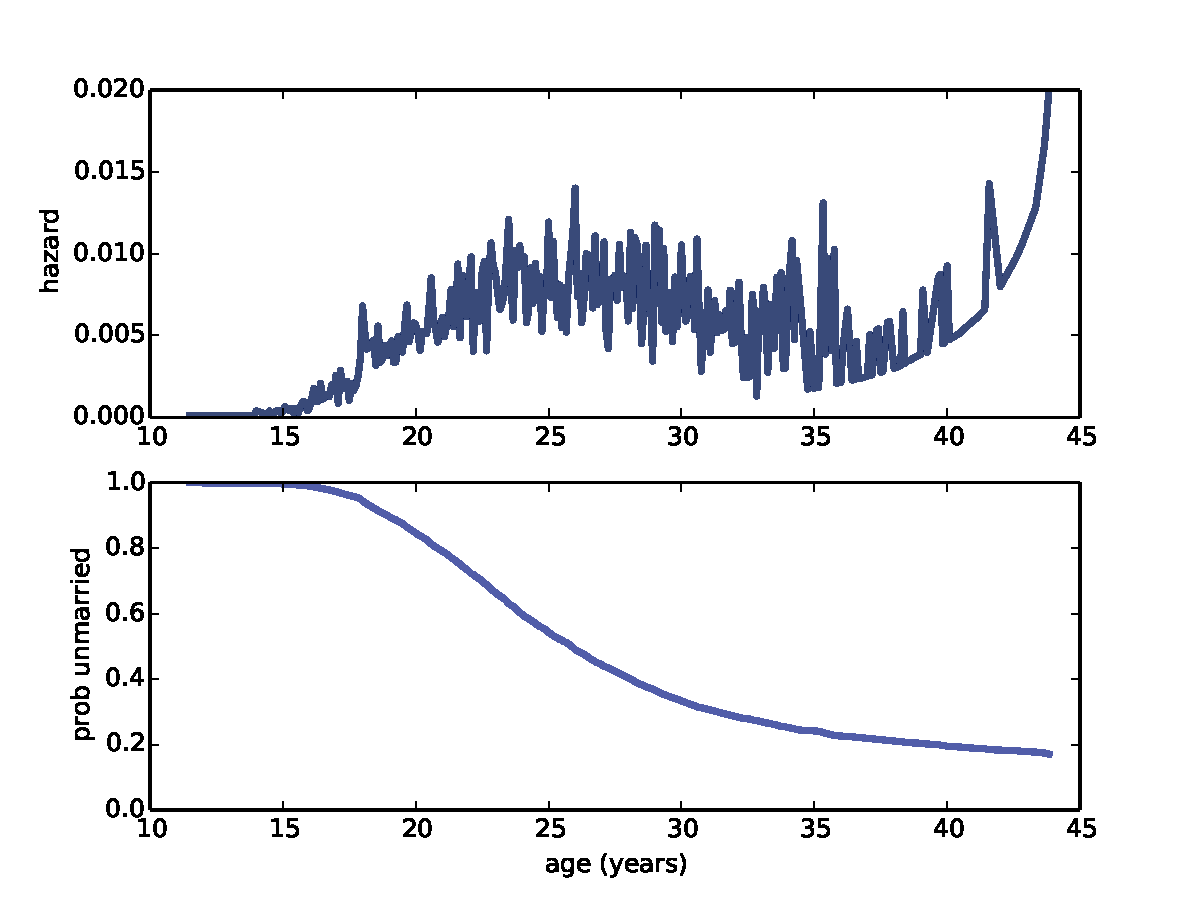
\includegraphics[height=2.5in]{figs/survival2.pdf}}
\caption{Hazard function for age at first marriage (top) and
survival curve (bottom).}
\label{survival2}
\end{figure}

Figure~\ref{survival2} (bottom) shows the result.  The survival
curve is steepest between 25 and 35, when most women get married.
Between 35 and 45,
the curve is nearly flat, indicating that women who do not marry
before age 35 are unlikely to get married.

A curve like this was the basis of a famous magazine article in 1986;
{\it Newsweek} reported that a 40-year old unmarried woman was ``more
likely to be killed by a terrorist'' than get married.  These
statistics were widely reported and became part of popular culture,
but they were wrong then (because they were based on faulty analysis)
and turned out to be even more wrong (because of cultural changes that
were already in progress and continued).  In 2006, {\it Newsweek} ran
an another article admitting that they were wrong.
\index{Newsweek}

I encourage you to read more about this article, the statistics it was
based on, and the reaction.  It should remind you of the ethical
obligation to perform statistical analysis with care, interpret the
results with appropriate skepticism, and present them to the public
accurately and honestly.
\index{ethics}


\section{Confidence intervals}

Kaplan-Meier analysis yields a single estimate of the survival curve,
but it is also important to quantify the uncertainty of the estimate.
As usual, there are three possible sources of error: measurement
error, sampling error, and modeling error.
\index{confidence interval}
\index{modeling error}
\index{sampling error}

In this example, measurement error is probably small.  People
generally know when they were born, whether they've been married, and
when.  And they can be expected to report this information accurately.
\index{measurement error}

We can quantify sampling error by resampling.  Here's the code:
\index{resampling}

\begin{verbatim}
def ResampleSurvival(resp, iters=101):
    low, high = resp.agemarry.min(), resp.agemarry.max()
    ts = np.arange(low, high, 1/12.0)

    ss_seq = []
    for i in range(iters):
        sample = thinkstats2.ResampleRowsWeighted(resp)
        hf, sf = EstimateSurvival(sample)
        ss_seq.append(sf.Probs(ts))

    low, high = thinkstats2.PercentileRows(ss_seq, [5, 95])
    thinkplot.FillBetween(ts, low, high)
\end{verbatim}

{\tt ResampleSurvival} takes {\tt resp}, a DataFrame of respondents,
and {\tt iters}, the number of times to resample.  It computes {\tt
  ts}, which is the sequence of ages where we will evaluate the survival
curves.
\index{DataFrame}

Inside the loop, {\tt ResampleSurvival}:

\begin{itemize}

\item Resamples the respondents using {\tt ResampleRowsWeighted},
which we saw in Section~\ref{weighted}.
\index{weighted resampling}

\item Calls {\tt EstimateSurvival}, which uses the process in the
previous sections to estimate the hazard and survival curves, and

\item Evaluates the survival curve at each age in {\tt ts}.

\end{itemize}

\verb"ss_seq" is a sequence of evaluated survival curves.
{\tt PercentileRows} takes this sequence and computes the 5th and 95th
percentiles, returning a 90\% confidence interval for the survival
curve.
\index{FillBetween}

\begin{figure}
% survival.py
\centerline{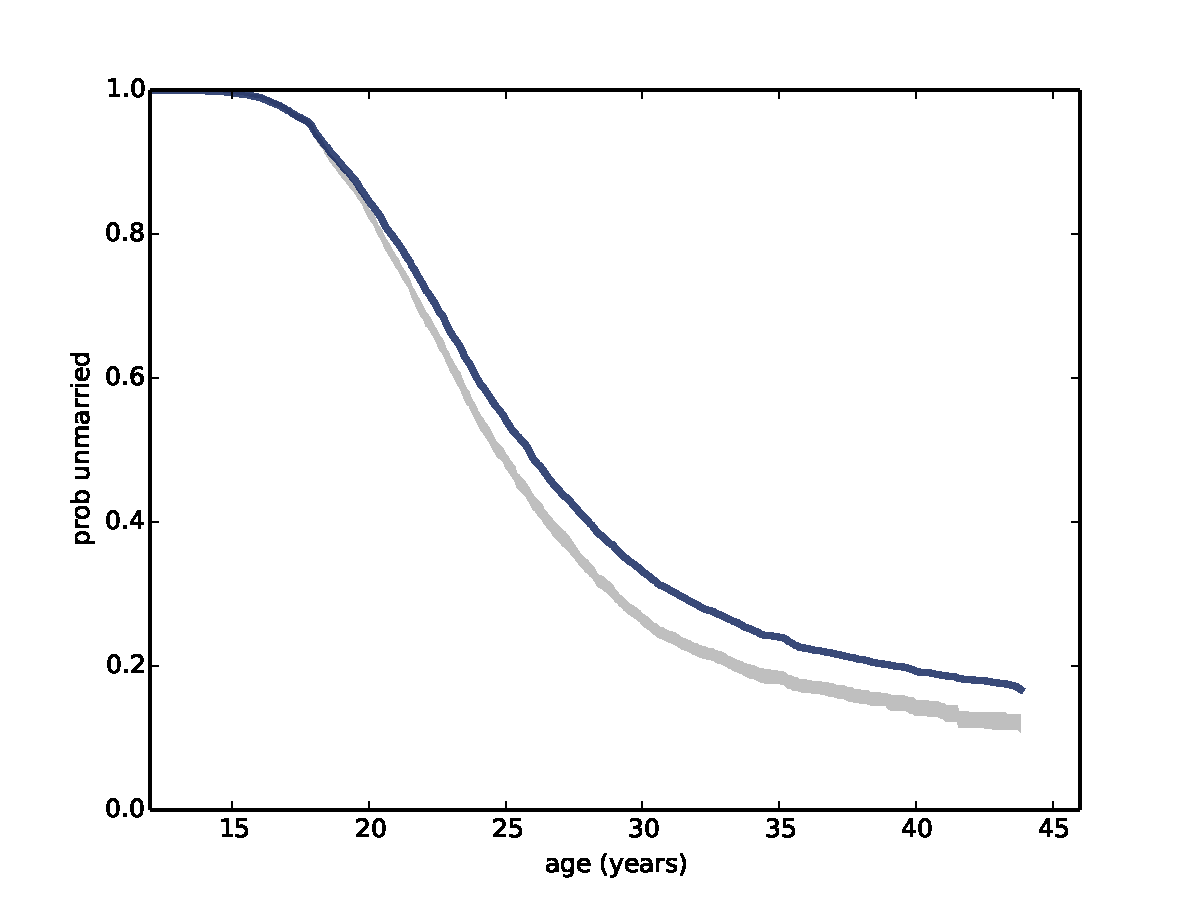
\includegraphics[height=2.5in]{figs/survival3.pdf}}
\caption{Survival curve for age at first marriage (dark line) and a 90\%
confidence interval based on weighted resampling (gray line).}
\label{survival3}
\end{figure}

Figure~\ref{survival3} shows the result along with the survival
curve we estimated in the previous section.  The confidence
interval takes into account the sampling weights, unlike the estimated
curve.  The discrepancy between them indicates that the sampling
weights have a substantial effect on the estimate---we will have
to keep that in mind.
\index{confidence interval}
\index{sampling weight}


\section{Cohort effects}

One of the challenges of survival analysis is that different parts
of the estimated curve are based on different groups of respondents.
The part of the curve at time {\tt t} is based on respondents
whose age was at least {\tt t} when they were interviewed.
So the leftmost part of the curve includes data from all respondents,
but the rightmost part includes only the oldest respondents.

If the relevant characteristics of the respondents are not changing
over time, that's fine, but in this case it seems likely that marriage
patterns are different for women born in different generations.
We can investigate this effect by grouping respondents according
to their decade of birth.  Groups like this, defined by date of
birth or similar events, are called {\bf cohorts}, and differences
between the groups are called {\bf cohort effects}.
\index{cohort}
\index{cohort effect}

To investigate cohort effects in the NSFG marriage data, I gathered
the Cycle 6 data from 2002 used throughout this book;
the Cycle 7 data from 2006--2010 used in Section~\ref{replication};
and the Cycle 5 data from 1995.  In total these datasets include
30,769 respondents.

\begin{verbatim}
    resp5 = ReadFemResp1995()
    resp6 = ReadFemResp2002()
    resp7 = ReadFemResp2010()
    resps = [resp5, resp6, resp7]
\end{verbatim}

For each DataFrame, {\tt resp}, I use {\tt cmbirth} to compute the
decade of birth for each respondent:
\index{pandas}
\index{DataFrame}

\begin{verbatim}
    month0 = pandas.to_datetime('1899-12-15')
    dates = [month0 + pandas.DateOffset(months=cm) 
             for cm in resp.cmbirth]
    resp['decade'] = (pandas.DatetimeIndex(dates).year - 1900) // 10
\end{verbatim}

{\tt cmbirth} is encoded as the integer number of months since
December 1899; {\tt month0} represents that date as a Timestamp
object.  For each birth date, we instantiate a {\tt DateOffset} that
contains the century-month and add it to {\tt month0}; the result
is a sequence of Timestamps, which is converted to a {\tt
  DateTimeIndex}.  Finally, we extract {\tt year} and compute
decades.
\index{DateTimeIndex}
\index{Index}
\index{century month}

To take into account the sampling weights, and also to show
variability due to sampling error, I resample the data,
group respondents by decade, and plot survival curves:
\index{resampling}
\index{sampling error}

\begin{verbatim}
    for i in range(iters):
        samples = [thinkstats2.ResampleRowsWeighted(resp) 
                   for resp in resps]
        sample = pandas.concat(samples, ignore_index=True)
        groups = sample.groupby('decade')

        EstimateSurvivalByDecade(groups, alpha=0.2)
\end{verbatim}

Data from the three NSFG cycles use different sampling weights,
so I resample them separately and then use {\tt concat}
to merge them into a single DataFrame.  The parameter \verb"ignore_index"
tells {\tt concat} not to match up respondents by index; instead
it creates a new index from 0 to 30768.
\index{pandas}
\index{DataFrame}
\index{groupby}

{\tt EstimateSurvivalByDecade} plots survival curves for each cohort:

\begin{verbatim}
def EstimateSurvivalByDecade(resp):
    for name, group in groups:
        hf, sf = EstimateSurvival(group)
        thinkplot.Plot(sf)
\end{verbatim}

\begin{figure}
% survival.py
\centerline{\includegraphics[height=2.5in]{figs/survival4.pdf}}
\caption{Survival curves for respondents born during different decades.}
\label{survival4}
\end{figure}

Figure~\ref{survival4} shows the results.  Several patterns are
visible:

\begin{itemize}

\item Women born in the 50s married earliest, with successive
  cohorts marrying later and later, at least until age 30 or so.

\item Women born in the 60s follow a surprising pattern.  Prior
to age 25, they were marrying at slower rates than their predecessors.
After age 25, they were marrying faster.  By age 32 they had overtaken
the 50s cohort, and at age 44 they are substantially more likely to
have married.
\index{marital status}

Women born in the 60s turned 25 between 1985 and 1995.  Remembering
that the {\it Newsweek} article I mentioned was published in 1986, it
is tempting to imagine that the article triggered a marriage boom.
That explanation would be too pat, but it is possible that the article
and the reaction to it were indicative of a mood that affected the
behavior of this cohort.
\index{Newsweek}

\item The pattern of the 70s cohort is similar.  They are less
likely than their predecessors to be married before age 25, but
at age 35 they have caught up with both of the previous cohorts.

\item Women born in the 80s are even less likely to marry before
age 25.  What happens after that is not clear; for more data, we
have to wait for the next cycle of the NSFG.

\end{itemize}

In the meantime we can make some predictions.
\index{prediction}


\section{Extrapolation}

The survival curve for the 70s cohort ends at about age 38;
for the 80s cohort it ends at age 28, and for the 90s cohort
we hardly have any data at all.
\index{extrapolation}

We can extrapolate these curves by ``borrowing'' data from the
previous cohort.  HazardFunction provides a method, {\tt Extend}, that
copies the tail from another longer HazardFunction:
\index{HazardFunction}

\begin{verbatim}
# class HazardFunction

    def Extend(self, other):
        last = self.series.index[-1]
        more = other.series[other.series.index > last]
        self.series = pandas.concat([self.series, more])
\end{verbatim}

As we saw in Section~\ref{hazard}, the HazardFunction contains a Series
that maps from $t$ to $\lambda(t)$.  {\tt Extend} finds {\tt last},
which is the last index in {\tt self.series}, selects values from
{\tt other} that come later than {\tt last}, and appends them
onto {\tt self.series}.
\index{pandas}
\index{Series}

Now we can extend the HazardFunction for each cohort, using values
from the predecessor:

\begin{verbatim}
def PlotPredictionsByDecade(groups):
    hfs = []
    for name, group in groups:
        hf, sf = EstimateSurvival(group)
        hfs.append(hf)

    thinkplot.PrePlot(len(hfs))
    for i, hf in enumerate(hfs):
        if i > 0:
            hf.Extend(hfs[i-1])
        sf = hf.MakeSurvival()
        thinkplot.Plot(sf)
\end{verbatim}

{\tt groups} is a GroupBy object with respondents grouped by decade of
birth.  The first loop computes the HazardFunction for each group.
\index{groupby}

The second loop extends each HazardFunction with values from
its predecessor, which might contain values from the previous
group, and so on.  Then it converts each HazardFunction to
a SurvivalFunction and plots it.

\begin{figure}
% survival.py
\centerline{\includegraphics[height=2.5in]{figs/survival5.pdf}}
\caption{Survival curves for respondents born during different decades,
with predictions for the later cohorts.}
\label{survival5}
\end{figure}

Figure~\ref{survival5} shows the results; I've removed the 50s cohort
to make the predictions more visible.  These results suggest that by
age 40, the most recent cohorts will converge with the 60s cohort,
with fewer than 20\% never married.
\index{visualization}


\section{Expected remaining lifetime}

Given a survival curve, we can compute the expected remaining
lifetime as a function of current age.  For example, given the
survival curve of pregnancy length from Section~\ref{survival},
we can compute the expected time until delivery.
\index{pregnancy length}

The first step is to extract the PMF of lifetimes.  {\tt SurvivalFunction}
provides a method that does that:

\begin{verbatim}
# class SurvivalFunction

    def MakePmf(self, filler=None):
        pmf = thinkstats2.Pmf()
        for val, prob in self.cdf.Items():
            pmf.Set(val, prob)

        cutoff = self.cdf.ps[-1]
        if filler is not None:
            pmf[filler] = 1-cutoff

        return pmf
\end{verbatim}

Remember that the SurvivalFunction contains the Cdf of lifetimes.
The loop copies the values and probabilities from the Cdf into
a Pmf.
\index{Pmf}
\index{Cdf}

{\tt cutoff} is the highest probability in the Cdf, which is 1
if the Cdf is complete, and otherwise less than 1.  
If the Cdf is incomplete, we plug in the provided value, {\tt filler},
to cap it off.

The Cdf of pregnancy lengths is complete, so we don't have to worry
about this detail yet.
\index{pregnancy length}

The next step is to compute the expected remaining lifetime, where
``expected'' means average.  {\tt SurvivalFunction}
provides a method that does that, too:
\index{expected remaining lifetime}

\begin{verbatim}
# class SurvivalFunction

    def RemainingLifetime(self, filler=None, func=thinkstats2.Pmf.Mean):
        pmf = self.MakePmf(filler=filler)
        d = {}
        for t in sorted(pmf.Values())[:-1]:
            pmf[t] = 0
            pmf.Normalize()
            d[t] = func(pmf) - t

        return pandas.Series(d)
\end{verbatim}

{\tt RemainingLifetime} takes {\tt filler}, which is passed along
to {\tt MakePmf}, and {\tt func} which is the function used to
summarize the distribution of remaining lifetimes.

{\tt pmf} is the Pmf of lifetimes extracted from the SurvivalFunction.
{\tt d} is a dictionary that contains the results, a map from
current age, {\tt t}, to expected remaining lifetime.
\index{Pmf}

The loop iterates through the values in the Pmf.  For each value
of {\tt t} it computes the conditional distribution of lifetimes,
given that the lifetime exceeds {\tt t}.  It does that by removing
values from the Pmf one at a time and renormalizing the remaining
values.

Then it uses {\tt func} to summarize the conditional distribution.
In this example the result is the mean pregnancy length, given that
the length exceeds {\tt t}.  By subtracting {\tt t} we get the
mean remaining pregnancy length.
\index{pregnancy length}

\begin{figure}
% survival.py
\centerline{\includegraphics[height=2.5in]{figs/survival6.pdf}}
\caption{Expected remaining pregnancy length (left) and
years until first marriage (right).}
\label{survival6}
\end{figure}

Figure~\ref{survival6} (left) shows the expected remaining pregnancy
length as a function of the current duration.  For example, during
Week 0, the expected remaining duration is about 34 weeks.  That's
less than full term (39 weeks) because terminations of pregnancy
in the first trimester bring the average down.
\index{pregnancy length}

The curve drops slowly during the first trimester.  After 13 weeks,
the expected remaining lifetime has dropped by only 9 weeks, to
25.  After that the curve drops faster, by about a week per week.

Between Week 37 and 42, the curve levels off between 1 and 2 weeks.
At any time during this period, the expected remaining lifetime is the
same; with each week that passes, the destination gets no closer.
Processes with this property are called {\bf memoryless} because
the past has no effect on the predictions.
This behavior is the mathematical basis of the infuriating mantra
of obstetrics nurses: ``any day now.''
\index{memoryless}

Figure~\ref{survival6} (right) shows the median remaining time until
first marriage, as a function of age.  For an 11 year-old girl, the
median time until first marriage is about 14 years.  The curve decreases
until age 22 when the median remaining time is about 7 years.
After that it increases again: by age 30 it is back where it started,
at 14 years.

Based on this data, young women have decreasing remaining
"lifetimes".  Mechanical components with this property are called {\bf NBUE}
for "new better than used in expectation," meaning that a new part is
expected to last longer.
\index{NBUE}

Women older than 22 have increasing remaining time until first
marriage.  Components with this property are called {\bf UBNE} for
"used better than new in expectation."  That is, the older the part,
the longer it is expected to last.  Newborns and cancer patients are
also UBNE; their life expectancy increases the longer they live.
\index{UBNE}

For this example I computed median, rather than mean, because the
Cdf is incomplete; the survival curve projects that about 20\%
of respondents will not marry before age 44.  The age of
first marriage for these women is unknown, and might be non-existent,
so we can't compute a mean.
\index{Cdf}
\index{median}

I deal with these unknown values by replacing them with {\tt np.inf},
a special value that represents infinity.  That makes the mean
infinity for all ages, but the median is well-defined as long as
more than 50\% of the remaining lifetimes are finite, which is true
until age 30.  After that it is hard to define a meaningful
expected remaining lifetime.
\index{inf}

Here's the code that computes and plots these functions:

\begin{verbatim}
    rem_life1 = sf1.RemainingLifetime()
    thinkplot.Plot(rem_life1)

    func = lambda pmf: pmf.Percentile(50)
    rem_life2 = sf2.RemainingLifetime(filler=np.inf, func=func)
    thinkplot.Plot(rem_life2)
\end{verbatim}

{\tt sf1} is the survival curve for pregnancy length;
in this case we can use the default values for {\tt RemainingLifetime}.
\index{pregnancy length}

{\tt sf2} is the survival curve for age at first marriage;
{\tt func} is a function that takes a Pmf and computes its
median (50th percentile).
\index{Pmf}


\section{Exercises}

My solution to this exercise is in \verb"chap13soln.py".

\begin{exercise}
In NSFG Cycles 6 and 7, the variable {\tt cmdivorcx} contains the
date of divorce for the respondent's first marriage, if applicable,
encoded in century-months.
\index{divorce}
\index{marital status}

Compute the duration of marriages that have ended in divorce, and
the duration, so far, of marriages that are ongoing.  Estimate the
hazard and survival curve for the duration of marriage.

Use resampling to take into account sampling weights, and plot
data from several resamples to visualize sampling error.
\index{resampling}

Consider dividing the respondents into groups by decade of birth,
and possibly by age at first marriage.
\index{groupby}

\end{exercise}


\section{Glossary}

\begin{itemize}

\item survival analysis: A set of methods for describing and
  predicting lifetimes, or more generally time until an event occurs.
\index{survival analysis}

\item survival curve: A function that maps from a time, $t$, to the
  probability of surviving past $t$.
\index{survival curve}

\item hazard function: A function that maps from $t$ to the fraction
of people alive until $t$ who die at $t$.
\index{hazard function}

\item Kaplan-Meier estimation: An algorithm for estimating hazard and
survival functions.
\index{Kaplan-Meier estimation}

\item cohort: a group of subjects defined by an event, like date of
birth, in a particular interval of time.
\index{cohort}

\item cohort effect: a difference between cohorts.
\index{cohort effect}

\item NBUE: A property of expected remaining lifetime, ``New
better than used in expectation.''
\index{NBUE}

\item UBNE: A property of expected remaining lifetime, ``Used
better than new in expectation.''
\index{UBNE}

\end{itemize}


\chapter{Analytic methods}
\label{analysis}

This book has focused on computational methods like simulation and
resampling, but some of the problems we solved have
analytic solutions that can be much faster.
\index{resampling}
\index{analytic methods}
\index{computational methods}

I present some of these methods in this chapter, and explain
how they work.  At the end of the chapter, I make suggestions
for integrating computational and analytic methods for exploratory
data analysis.

The code in this chapter is in {\tt normal.py}.  For information
about downloading and working with this code, see Section~\ref{code}.


\section{Normal distributions}
\label{why_normal}
\index{normal distribution}
\index{distribution!normal}
\index{Gaussian distribution}
\index{distribution!Gaussian}

As a motivating example, let's review the problem from
Section~\ref{gorilla}:
\index{gorilla}

\begin{quotation}
\noindent Suppose you are a scientist studying gorillas in a wildlife
preserve.  Having weighed 9 gorillas, you find sample mean $\xbar=90$ kg and
sample standard deviation, $S=7.5$ kg.  If you use $\xbar$ to estimate
the population mean, what is the standard error of the estimate?
\end{quotation}

To answer that question, we need the sampling
distribution of $\xbar$.  In Section~\ref{gorilla} we approximated
this distribution by simulating the experiment (weighing
9 gorillas), computing $\xbar$ for each simulated experiment, and
accumulating the distribution of estimates.
\index{standard error}
\index{standard deviation}

The result is an approximation of the sampling distribution.  Then we
use the sampling distribution to compute standard errors and
confidence intervals:
\index{confidence interval}
\index{sampling distribution}

\begin{enumerate}

\item The standard deviation of the sampling distribution is the
  standard error of the estimate; in the example, it is about
  2.5 kg.

\item The interval between the 5th and 95th percentile of the sampling
  distribution is a 90\% confidence interval.  If we run the
  experiment many times, we expect the estimate to fall in this
  interval 90\% of the time.  In the example, the 90\% CI is
  $(86, 94)$ kg.

\end{enumerate}

Now we'll do the same calculation analytically.  We
take advantage of the fact that the weights of adult female gorillas
are roughly normally distributed.  Normal distributions have two
properties that make them amenable for analysis: they are ``closed'' under
linear transformation and addition.  To explain what that means, I
need some notation.  \index{analysis}
\index{linear transformation}
\index{addition, closed under}

If the distribution of a quantity, $X$, is
normal with parameters $\mu$ and $\sigma$, you can write
%
\[ X \sim \normal~(\mu, \sigma^{2})\]
%
where the symbol $\sim$ means ``is distributed'' and the script letter
$\normal$ stands for ``normal.''

%The other analytic distributions in this chapter are sometimes
%written $\mathrm{Exponential}(\lambda)$, $\mathrm{Pareto}(x_m,
%\alpha)$ and, for lognormal, $\mathrm{Log}-\normal~(\mu,
%\sigma^2)$.

A linear transformation of $X$ is something like $X' = a X + b$, where
$a$ and $b$ are real numbers.\index{linear transformation}
A family of distributions is closed under
linear transformation if $X'$ is in the same family as $X$.  The normal
distribution has this property; if $X \sim \normal~(\mu,
\sigma^2)$,
%
\[ X' \sim \normal~(a \mu + b, a^{2} \sigma^2) \tag*{(1)} \]
%
Normal distributions are also closed under addition.  
If $Z = X + Y$ and
$X \sim \normal~(\mu_{X}, \sigma_{X}^{2})$ and
$Y \sim \normal~(\mu_{Y}, \sigma_{Y}^{2})$ then
%
\[ Z \sim \normal~(\mu_X + \mu_Y, \sigma_X^2 + \sigma_Y^2)  \tag*{(2)}\]
%
In the special case $Z = X + X$, we have
%
\[ Z \sim \normal~(2 \mu_X, 2 \sigma_X^2) \]
%
and in general if we draw $n$ values of $X$ and add them up, we have
%
\[ Z \sim \normal~(n \mu_X, n \sigma_X^2)  \tag*{(3)}\]


\section{Sampling distributions}

Now we have everything we need to compute the sampling distribution of
$\xbar$.  Remember that we compute $\xbar$ by weighing $n$ gorillas,
adding up the total weight, and dividing by $n$.
\index{sampling distribution}
\index{gorilla}
\index{weight}

Assume that the distribution of gorilla weights, $X$, is
approximately normal:
%
\[ X \sim \normal~(\mu, \sigma^2)\]
%
If we weigh $n$ gorillas, the total weight, $Y$, is distributed
%
\[ Y \sim \normal~(n \mu, n \sigma^2) \]
%
using Equation 3.  And if we divide by $n$, the sample mean,
$Z$, is distributed
%
\[ Z \sim \normal~(\mu, \sigma^2/n) \]
%
using Equation 1 with $a = 1/n$.

The distribution of $Z$ is the sampling distribution of $\xbar$.
The mean of $Z$ is $\mu$, which shows that $\xbar$ is an unbiased
estimate of $\mu$.  The variance of the sampling distribution
is $\sigma^2 / n$.
\index{biased estimator}
\index{estimator!biased}

So the standard deviation of the sampling distribution, which is the
standard error of the estimate, is $\sigma / \sqrt{n}$.  In the
example, $\sigma$ is 7.5 kg and $n$ is 9, so the standard error is 2.5
kg.  That result is consistent with what we estimated by simulation,
but much faster to compute!
\index{standard error}
\index{standard deviation}

We can also use the sampling distribution to compute confidence
intervals.  A 90\% confidence interval for $\xbar$ is the interval
between the 5th and 95th percentiles of $Z$.  Since $Z$ is normally
distributed, we can compute percentiles by evaluating the inverse
CDF.
\index{inverse CDF}
\index{CDF, inverse}
\index{confidence interval}

There is no closed form for the CDF of the normal distribution
or its inverse, but there are fast numerical methods and they
are implemented in SciPy, as we saw in Section~\ref{normal}.
{\tt thinkstats2} provides a wrapper function that makes the
SciPy function a little easier to use:
\index{SciPy}
\index{normal distribution}
\index{wrapper}
\index{closed form}

\begin{verbatim}
def EvalNormalCdfInverse(p, mu=0, sigma=1):
    return scipy.stats.norm.ppf(p, loc=mu, scale=sigma)
\end{verbatim}

Given a probability, {\tt p}, it returns the corresponding
percentile from a normal distribution with parameters {\tt mu}
and {\tt sigma}.  For the 90\% confidence interval of $\xbar$,
we compute the 5th and 95th percentiles like this:
\index{percentile}

\begin{verbatim}
>>> thinkstats2.EvalNormalCdfInverse(0.05, mu=90, sigma=2.5)
85.888

>>> thinkstats2.EvalNormalCdfInverse(0.95, mu=90, sigma=2.5)
94.112
\end{verbatim}

So if we run the experiment many times, we expect the
estimate, $\xbar$, to fall in the range $(85.9, 94.1)$ about
90\% of the time.  Again, this is consistent with the result
we got by simulation.
\index{simulation}


\section{Representing normal distributions}

To make these calculations easier, I have defined a class called
{\tt Normal} that represents a normal distribution and encodes
the equations in the previous sections.  Here's what it looks
like:
\index{Normal}

\begin{verbatim}
class Normal(object):

    def __init__(self, mu, sigma2):
        self.mu = mu
        self.sigma2 = sigma2

    def __str__(self):
        return 'N(%g, %g)' % (self.mu, self.sigma2)
\end{verbatim}

So we can instantiate a Normal that represents the distribution
of gorilla weights:
\index{gorilla}

\begin{verbatim}
>>> dist = Normal(90, 7.5**2)
>>> dist
N(90, 56.25)
\end{verbatim}

{\tt Normal} provides {\tt Sum}, which takes a sample size, {\tt n},
and returns the distribution of the sum of {\tt n} values, using
Equation 3:

\begin{verbatim}
    def Sum(self, n):
        return Normal(n * self.mu, n * self.sigma2)
\end{verbatim}

Normal also knows how to multiply and divide using
Equation 1:

\begin{verbatim}
    def __mul__(self, factor):
        return Normal(factor * self.mu, factor**2 * self.sigma2)

    def __div__(self, divisor):
        return 1 / divisor * self
\end{verbatim}

So we can compute the sampling distribution of the mean with sample
size 9:
\index{sampling distribution}
\index{sample size}

\begin{verbatim}
>>> dist_xbar = dist.Sum(9) / 9
>>> dist_xbar.sigma
2.5
\end{verbatim}

The standard deviation of the sampling distribution is 2.5 kg, as we
saw in the previous section.  Finally, Normal provides {\tt
  Percentile}, which we can use to compute a confidence interval:
\index{standard deviation}
\index{confidence interval}

\begin{verbatim}
>>> dist_xbar.Percentile(5), dist_xbar.Percentile(95)
85.888 94.113
\end{verbatim}

And that's the same answer we got before.  We'll use the Normal
class again later, but before we go on, we need one more bit of
analysis.


\section{Central limit theorem}
\label{CLT}

As we saw in the previous sections, if we add values drawn from normal
distributions, the distribution of the sum is normal.
Most other distributions don't have this property;
if we add values drawn from other distributions, the sum does not
generally have an analytic distribution.
  \index{sum}
\index{normal distribution} \index{distribution!normal}
\index{Gaussian distribution} \index{distribution!Gaussian}

But if we add up {\tt n} values from
almost any distribution, the distribution of the sum converges to
normal as {\tt n} increases.

More specifically, if the distribution of the values has mean and
standard deviation $\mu$ and $\sigma$, the distribution of the sum is
approximately $\normal(n \mu, n \sigma^2)$.
\index{standard deviation}

This result is the Central Limit Theorem (CLT).  It is one of the
most useful tools for statistical analysis, but it comes with
caveats:
\index{Central Limit Theorem}
\index{CLT}

\begin{itemize}

\item The values have to be drawn independently.  If they are
correlated, the CLT doesn't apply (although this is seldom a problem
in practice).
\index{independent}

\item The values have to come from the same distribution (although
  this requirement can be relaxed).
\index{identical}

\item The values have to be drawn
  from a distribution with finite mean and variance.  So most Pareto
  distributions are out.
\index{mean}
\index{variance}
\index{Pareto distribution}
\index{distribution!Pareto}
\index{exponential distribution}
\index{distribution!exponential}

\item The rate of convergence depends
  on the skewness of the distribution.  Sums from an exponential
  distribution converge for small {\tt n}.  Sums from a
  lognormal distribution require larger sizes.
\index{lognormal distribution}
\index{distribution!lognormal}
\index{skewness}

\end{itemize}

The Central Limit Theorem explains the prevalence
of normal distributions in the natural world.  Many characteristics of
living things are affected by genetic
and environmental factors whose effect is additive.  The characteristics
we measure are the sum of a large number of small effects, so their
distribution tends to be normal.
\index{normal distribution}
\index{distribution!normal}
\index{Gaussian distribution}
\index{distribution!Gaussian}
\index{Central Limit Theorem}
\index{CLT}


\section{Testing the CLT}

To see how the Central Limit Theorem works, and when it doesn't,
let's try some experiments.  First, we'll try
an exponential distribution:

\begin{verbatim}
def MakeExpoSamples(beta=2.0, iters=1000):
    samples = []
    for n in [1, 10, 100]:
        sample = [np.sum(np.random.exponential(beta, n))
                  for _ in range(iters)]
        samples.append((n, sample))
    return samples
\end{verbatim}

{\tt MakeExpoSamples} generates samples of sums of exponential values
(I use ``exponential values'' as shorthand for ``values from an
exponential distribution'').
{\tt beta} is the parameter of the distribution; {\tt iters}
is the number of sums to generate.

To explain this function, I'll start from the inside and work my way
out.  Each time we call {\tt np.random.exponential}, we get a sequence
of {\tt n} exponential values and compute its sum.  {\tt sample}
is a list of these sums, with length {\tt iters}.
\index{NumPy}

It is easy to get {\tt n} and {\tt iters} confused:  {\tt n} is the
number of terms in each sum;  {\tt iters} is the number of sums we
compute in order to characterize the distribution of sums.

The return value is a list of {\tt (n, sample)} pairs.  For
each pair, we make a normal probability plot:
\index{thinkplot}
\index{normal probability plot}

\begin{verbatim}
def NormalPlotSamples(samples, plot=1, ylabel=''):
    for n, sample in samples:
        thinkplot.SubPlot(plot)
        thinkstats2.NormalProbabilityPlot(sample)

        thinkplot.Config(title='n=%d' % n, ylabel=ylabel)
        plot += 1
\end{verbatim}

{\tt NormalPlotSamples} takes the list of pairs from {\tt
  MakeExpoSamples} and generates a row of normal probability plots.
\index{normal probability plot}

\begin{figure}
% normal.py
\centerline{\includegraphics[height=3.5in]{figs/normal1.pdf}}
\caption{Distributions of sums of exponential values (top row) and
lognormal values (bottom row).}
\label{normal1}
\end{figure}

Figure~\ref{normal1} (top row) shows
the results.  With {\tt n=1}, the distribution of the sum is still
exponential, so the normal probability plot is not a straight line.
But with {\tt n=10} the distribution of the sum is approximately
normal, and with {\tt n=100} it is all but indistinguishable from
normal.

Figure~\ref{normal1} (bottom row) shows similar results for a
lognormal distribution.  Lognormal distributions are generally more
skewed than exponential distributions, so the distribution of sums
takes longer to converge.  With {\tt n=10} the normal
probability plot is nowhere near straight, but with {\tt n=100}
it is approximately normal.
\index{lognormal distribution}
\index{distribution!lognormal}
\index{skewness}

\begin{figure}
% normal.py
\centerline{\includegraphics[height=3.5in]{figs/normal2.pdf}}
\caption{Distributions of sums of Pareto values (top row) and
correlated exponential values (bottom row).}
\label{normal2}
\end{figure}

Pareto distributions are even more skewed than lognormal.  Depending
on the parameters, many Pareto distributions do not have finite mean
and variance.  As a result, the Central Limit Theorem does not apply.
Figure~\ref{normal2} (top row) shows distributions of sums of
Pareto values.  Even with {\tt n=100} the normal probability plot
is far from straight.
\index{Pareto distribution}
\index{distribution!Pareto}
\index{Central Limit Theorem}
\index{CLT}
\index{normal probability plot}

I also mentioned that CLT does not apply if the values are correlated.
To test that, I generate correlated values from an exponential
distribution.  The algorithm for generating correlated values is
(1) generate correlated normal values, (2) use the normal CDF
to transform the values to uniform, and (3) use the inverse
exponential CDF to transform the uniform values to exponential.
\index{inverse CDF}
\index{CDF, inverse}
\index{correlation}
\index{random number}

{\tt GenerateCorrelated} returns an iterator of {\tt n} normal values
with serial correlation {\tt rho}:
\index{iterator}

\begin{verbatim}
def GenerateCorrelated(rho, n):
    x = random.gauss(0, 1)
    yield x

    sigma = math.sqrt(1 - rho**2)
    for _ in range(n-1):
        x = random.gauss(x*rho, sigma)
        yield x
\end{verbatim}

The first value is a standard normal value.  Each subsequent value
depends on its predecessor: if the previous value is {\tt x}, the mean of
the next value is {\tt x*rho}, with variance {\tt 1-rho**2}.  Note that {\tt
  random.gauss} takes the standard deviation as the second argument,
not variance.
\index{standard deviation}
\index{standard normal distribution}

{\tt GenerateExpoCorrelated}
takes the resulting sequence and transforms it to exponential:

\begin{verbatim}
def GenerateExpoCorrelated(rho, n):
    normal = list(GenerateCorrelated(rho, n))
    uniform = scipy.stats.norm.cdf(normal)
    expo = scipy.stats.expon.ppf(uniform)
    return expo
\end{verbatim}

{\tt normal} is a list of correlated normal values.  {\tt uniform}
is a sequence of uniform values between 0 and 1.  {\tt expo} is
a correlated sequence of exponential values.
{\tt ppf} stands for ``percent point function,'' which is another
name for the inverse CDF.
\index{inverse CDF}
\index{CDF, inverse}
\index{percent point function}

Figure~\ref{normal2} (bottom row) shows distributions of sums of
correlated exponential values with {\tt rho=0.9}.  The correlation
slows the rate of convergence; nevertheless, with {\tt n=100} the
normal probability plot is nearly straight.  So even though CLT
does not strictly apply when the values are correlated, moderate
correlations are seldom a problem in practice.
\index{normal probability plot}
\index{correlation}

These experiments are meant to show how the Central Limit Theorem
works, and what happens when it doesn't.  Now let's see how we can
use it.


\section{Applying the CLT}
\label{usingCLT}

To see why the Central Limit Theorem is useful, let's get back
to the example in Section~\ref{testdiff}: testing the apparent
difference in mean pregnancy length for first babies and others.
As we've seen, the apparent difference is about
0.078 weeks:
\index{pregnancy length}
\index{Central Limit Theorem}
\index{CLT}

\begin{verbatim}
>>> live, firsts, others = first.MakeFrames()
>>> delta = firsts.prglngth.mean() - others.prglngth.mean()
0.078
\end{verbatim}

Remember the logic of hypothesis testing: we compute a p-value, which
is the probability of the observed difference under the null
hypothesis; if it is small, we conclude that the observed difference
is unlikely to be due to chance.
\index{p-value}
\index{null hypothesis}
\index{hypothesis testing}

In this example, the null hypothesis is that the distribution of
pregnancy lengths is the same for first babies and others.  
So we can compute the sampling distribution of the mean
like this:
\index{sampling distribution}

\begin{verbatim}
    dist1 = SamplingDistMean(live.prglngth, len(firsts))
    dist2 = SamplingDistMean(live.prglngth, len(others))
\end{verbatim}

Both sampling distributions are based on the same population, which is
the pool of all live births.  {\tt SamplingDistMean} takes this
sequence of values and the sample size, and returns a Normal object
representing the sampling distribution:

\begin{verbatim}
def SamplingDistMean(data, n):
    mean, var = data.mean(), data.var()
    dist = Normal(mean, var)
    return dist.Sum(n) / n
\end{verbatim}

{\tt mean} and {\tt var} are the mean and variance of
{\tt data}.  We approximate the distribution of the data with
a normal distribution, {\tt dist}.  

In this example, the data are not normally distributed, so this
approximation is not very good.  But then we compute {\tt dist.Sum(n)
  / n}, which is the sampling distribution of the mean of {\tt n}
values.  Even if the data are not normally distributed, the sampling
distribution of the mean is, by the Central Limit Theorem.
\index{Central Limit Theorem}
\index{CLT}

Next, we compute the sampling distribution of the difference
in the means.  The {\tt Normal} class knows how to perform
subtraction using Equation 2:
\index{Normal}

\begin{verbatim}
    def __sub__(self, other):
        return Normal(self.mu - other.mu,
                      self.sigma2 + other.sigma2)
\end{verbatim}

So we can compute the sampling distribution of the difference like this:

\begin{verbatim}
>>> dist = dist1 - dist2
N(0, 0.0032)
\end{verbatim}

The mean is 0, which makes sense because we expect two samples from
the same distribution to have the same mean, on average.  The variance
of the sampling distribution is 0.0032.
\index{sampling distribution}

{\tt Normal} provides {\tt Prob}, which evaluates the normal CDF.
We can use {\tt Prob} to compute the probability of a
difference as large as {\tt delta} under the null hypothesis:
\index{null hypothesis}

\begin{verbatim}
>>> 1 - dist.Prob(delta)
0.084
\end{verbatim}

Which means that the p-value for a one-sided test is 0.84.  For
a two-sided test we would also compute
\index{p-value}
\index{one-sided test}
\index{two-sided test}

\begin{verbatim}
>>> dist.Prob(-delta)
0.084
\end{verbatim}

Which is the same because the normal distribution is symmetric.
The sum of the tails is 0.168, which is consistent with the estimate
in Section~\ref{testdiff}, which was 0.17.
\index{symmetric}



\section{Correlation test}

In Section~\ref{corrtest} we used a permutation test for the correlation
between birth weight and mother's age, and found that it is
statistically significant, with p-value less than 0.001.
\index{p-value}
\index{birth weight}
\index{weight!birth}
\index{permutation}
  \index{significant} \index{statistically significant}

Now we can do the same thing analytically.  The method is based
on this mathematical result: given two variables that are normally distributed
and uncorrelated, if we generate a sample with size $n$,
compute Pearson's correlation, $r$, and then compute the transformed
correlation
%
\[ t = r \sqrt{\frac{n-2}{1-r^2}} \]
%
the distribution of $t$ is Student's t-distribution with parameter
$n-2$.  The t-distribution is an analytic distribution; the CDF can
be computed efficiently using gamma functions.
\index{Pearson coefficient of correlation}
\index{correlation}

We can use this result to compute the sampling distribution of
correlation under the null hypothesis; that is, if we generate
uncorrelated sequences of normal values, what is the distribution of
their correlation?  {\tt StudentCdf} takes the sample size, {\tt n}, and
returns the sampling distribution of correlation:
\index{null hypothesis}
\index{sampling distribution}

\begin{verbatim}
def StudentCdf(n):
    ts = np.linspace(-3, 3, 101)
    ps = scipy.stats.t.cdf(ts, df=n-2)
    rs = ts / np.sqrt(n - 2 + ts**2)
    return thinkstats2.Cdf(rs, ps)
\end{verbatim}

{\tt ts} is a NumPy array of values for $t$, the transformed
correlation.  {\tt ps} contains the corresponding probabilities,
computed using the CDF of the Student's t-distribution implemented in
SciPy.  The parameter of the t-distribution, {\tt df}, stands for
``degrees of freedom.''  I won't explain that term, but you can read
about it at
\url{http://en.wikipedia.org/wiki/Degrees_of_freedom_(statistics)}.
\index{NumPy}
\index{SciPy}
\index{Student's t-distribution}
\index{distribution!Student's t}
\index{degrees of freedom}

\begin{figure}
% normal.py
\centerline{\includegraphics[height=2.5in]{figs/normal4.pdf}}
\caption{Sampling distribution of correlations for uncorrelated
normal variables.}
\label{normal4}
\end{figure}

To get from {\tt ts} to the correlation coefficients, {\tt rs},
we apply the inverse transform,
%
\[ r = t / \sqrt{n - 2 + t^2} \]
%
The result is the sampling distribution of $r$ under the null hypothesis.
Figure~\ref{normal4} shows this distribution along with the distribution
we generated in Section~\ref{corrtest} by resampling.  They are nearly
identical.  Although the actual distributions are not normal, 
Pearson's coefficient of correlation is based on sample means
and variances.  By the Central Limit Theorem, these moment-based
statistics are normally distributed even if the data are not.
\index{Central Limit Theorem}
\index{CLT}
\index{null hypothesis}
\index{resampling}

From Figure~\ref{normal4}, we can see that the
observed correlation, 0.07, is unlikely to occur if the variables
are actually uncorrelated.
Using the analytic distribution, we can compute just how unlikely:
\index{analytic distribution}

\begin{verbatim}
    t = r * math.sqrt((n-2) / (1-r))
    p_value = 1 - scipy.stats.t.cdf(t, df=n-2)
\end{verbatim}

We compute the value of {\tt t} that corresponds to {\tt r=0.07}, and
then evaluate the t-distribution at {\tt t}.  The result is {\tt
  6.4e-12}.  This example demonstrates an advantage of the analytic
method: we can compute very small p-values.  But in practice it
usually doesn't matter.
\index{SciPy}
\index{p-value}


\section{Chi-squared test}

In Section~\ref{casino2} we used the chi-squared statistic to
test whether a die is crooked.  The chi-squared statistic measures
the total normalized deviation from the expected values in a table:
%
\[ \goodchi^2 = \sum_i \frac{(O_i - E_i)^2}{E_i} \]
%
One reason the chi-squared statistic is widely used is that
its sampling distribution under the null hypothesis is analytic;
by a remarkable coincidence\footnote{Not really.}, it is called
the chi-squared distribution.  Like the t-distribution, the
chi-squared CDF can be computed efficiently using gamma functions.
\index{deviation}
\index{null hypothesis}
\index{sampling distribution}
\index{chi-squared test}
\index{chi-squared distribution}
\index{distribution!chi-squared}

\begin{figure}
% normal.py
\centerline{\includegraphics[height=2.5in]{figs/normal5.pdf}}
\caption{Sampling distribution of chi-squared statistics for
a fair six-sided die.}
\label{normal5}
\end{figure}

SciPy provides an implementation of the chi-squared distribution,
which we use to compute the sampling distribution of the
chi-squared statistic:
\index{SciPy}

\begin{verbatim}
def ChiSquaredCdf(n):
    xs = np.linspace(0, 25, 101)
    ps = scipy.stats.chi2.cdf(xs, df=n-1)
    return thinkstats2.Cdf(xs, ps)
\end{verbatim}

Figure~\ref{normal5} shows the analytic result along with the
distribution we got by resampling.  They are very similar,
especially in the tail, which is the part we usually care most
about.
\index{resampling}
\index{tail}

We can use this distribution to compute the p-value of the
observed test statistic, {\tt chi2}:
\index{test statistic}
\index{p-value}

\begin{verbatim}
    p_value = 1 - scipy.stats.chi2.cdf(chi2, df=n-1)
\end{verbatim}

The result is 0.041, which is consistent with the result
from Section~\ref{casino2}.

The parameter of the chi-squared distribution is ``degrees of
freedom'' again.  In this case the correct parameter is {\tt n-1},
where {\tt n} is the size of the table, 6.  Choosing this parameter
can be tricky; to be honest, I am never confident that I have it
right until I generate something like Figure~\ref{normal5} to compare
the analytic results to the resampling results.
\index{degrees of freedom}


\section{Discussion}

This book focuses on computational methods like resampling and
permutation.  These methods have several advantages over analysis:
\index{resampling}
\index{permutation}
\index{computational methods}

\begin{itemize}

\item They are easier to explain and understand.  For example, one of
  the most difficult topics in an introductory statistics class is
  hypothesis testing.  Many students don't really understand what
  p-values are.  I think the approach I presented in
  Chapter~\ref{testing}---simulating the null hypothesis and
  computing test statistics---makes the fundamental idea clearer.
\index{p-value}
\index{null hypothesis}

\item They are robust and versatile.  Analytic methods are often based
  on assumptions that might not hold in practice.  Computational
  methods require fewer assumptions, and can be adapted and extended
  more easily.
\index{robust}

\item They are debuggable.  Analytic methods are often like a black
  box: you plug in numbers and they spit out results.  But it's easy
  to make subtle errors, hard to be confident that the results are
  right, and hard to find the problem if they are not.  Computational
  methods lend themselves to incremental development and testing,
  which fosters confidence in the results.
\index{debugging}

\end{itemize}

But there is one drawback: computational methods can be slow.  Taking
into account these pros and cons, I recommend the following process:

\begin{enumerate}

\item Use computational methods during exploration.  If you find a
  satisfactory answer and the run time is acceptable, you can stop.
\index{exploration}

\item If run time is not acceptable, look for opportunities to
  optimize.  Using analytic methods is one of several methods of
  optimization.

\item If replacing a computational method with an analytic method is
  appropriate, use the computational method as a basis of comparison, 
  providing mutual validation between the computational and
  analytic results.
\index{model}

\end{enumerate}

For the vast majority of problems I have worked on, I didn't have
to go past Step 1.


\section{Exercises}

A solution to these exercises is in \verb"chap14soln.py"

\begin{exercise}
\label{log_clt}
In Section~\ref{lognormal}, we saw that the distribution
of adult weights is approximately lognormal.  One possible
explanation is that the weight a person
gains each year is proportional to their current weight.
In that case, adult weight is the product of a large number
of multiplicative factors:
%
\[ w = w_0 f_1 f_2 ... f_n  \]
%
where $w$ is adult weight, $w_0$ is birth weight, and $f_i$
is the weight gain factor for year $i$.
\index{birth weight}
\index{weight!birth}
\index{lognormal distribution}
\index{distribution!lognormal}
\index{adult weight}

The log of a product is the sum of the logs of the
factors:
%
\[ \log w = \log w_0 + \log f_1 + \log f_2 + ... + \log f_n \]
%
So by the Central Limit Theorem, the distribution of $\log w$ is
approximately normal for large $n$, which implies that the
distribution of $w$ is lognormal.
\index{Central Limit Theorem}
\index{CLT}

To model this phenomenon, choose a distribution for $f$ that seems
reasonable, then generate a sample of adult weights by choosing a
random value from the distribution of birth weights, choosing a
sequence of factors from the distribution of $f$, and computing the
product.  What value of $n$ is needed to converge to a lognormal
distribution?
\index{model}

\index{logarithm}
\index{product}

\end{exercise}



\begin{exercise}
In Section~\ref{usingCLT} we used the Central Limit Theorem to find
the sampling distribution of the difference in means, $\delta$, under
the null hypothesis that both samples are drawn from the same
population.
\index{null hypothesis}
\index{sampling distribution}

We can also use this distribution to find the standard error of the
estimate and confidence intervals, but that would only be
approximately correct.  To be more precise, we should compute the
sampling distribution of $\delta$ under the alternate hypothesis that
the samples are drawn from different populations.
\index{standard error}
\index{standard deviation}
\index{confidence interval}

Compute this distribution and use it to calculate the standard error
and a 90\% confidence interval for the difference in means.
\end{exercise}


\begin{exercise}
In a recent paper\footnote{``Evidence for the persistent effects of an
  intervention to mitigate gender-sterotypical task allocation within
  student engineering teams,'' Proceedings of the IEEE Frontiers in Education
Conference, 2014.}, Stein et al.~investigate the
effects of an intervention intended to mitigate gender-stereotypical
task allocation within student engineering teams.

Before and after the intervention, students responded to a survey that
asked them to rate their contribution to each aspect of class projects on
a 7-point scale.

Before the intervention, male students reported higher scores for the
programming aspect of the project than female students; on average men
reported a score of 3.57 with standard error 0.28.  Women reported
1.91, on average, with standard error 0.32.
\index{standard error}

Compute the sampling distribution of the gender gap (the difference in
means), and test whether it is statistically significant.  Because you
are given standard errors for the estimated means, you don't need to
know the sample size to figure out the sampling distributions.
  \index{significant} \index{statistically significant}
\index{sampling distribution}

After the intervention, the gender gap was smaller: the average score
for men was 3.44 (SE 0.16); the average score for women was 3.18 (SE
0.16).  Again, compute the sampling distribution of the gender gap and
test it.
\index{gender gap}

Finally, estimate the change in gender gap; what is the sampling
distribution of this change, and is it statistically significant?
  \index{significant} \index{statistically significant}
\end{exercise}


\printindex

\clearemptydoublepage
%\blankpage
%\blankpage
%\blankpage


\end{document}


